\باب{لامتناہی تسلسل}\شناخت{باب_لامتناہی_تسلسل}
اس باب میں ہم ایک حیران کن کلیہ اخذ کرتے ہیں جس کی مدد سے بہت سارے تفاعل کو "لامتناہی کثیر رکنی" کی صورت میں لکھنا ممکن ہو گا اور ساتھ ہی کثیر رکنی کے  ارکان حذف  کر کے کثیر رکنی کو متناہی بنانے سے پیدا خلل بھی جان پائیں گے۔ ان تسلسل کو طاقتی تسلسل کہتے ہیں۔ قابل تفرق تفاعل کو تخمینی طور پر کثیر رکنی سے ظاہر کرنے میں مدد دینے کے علاوہ طاقتی تسلسل دیگر مواقع پر بھی کار آمد ثابت ہوتے ہیں۔ غیر بنیادی تکمل کی قیمت کے حصول کے علاوہ حراری توانائی کی منتقلی، ارتعاش، کیمیائی نفوذ اور ترسیل اشارات کے تفرقی مساوات  کے حل میں یہ موثر کردار ادا کرتے ہیں۔ آپ یہاں وہ ان تفاعل کے بارے میں سیکھ پائیں گے جو سائن اور انجینئری میں بہت زیادہ استعمال ہوتے ہیں۔

\حصہ{اعداد کی ترتیب کی حد}
غیر رسمی طور پر ترتیب سے مراد مرتب چیزوں کا سلسلہ ہے۔ اس باب میں ہمیں اعداد کی ترتیب سے غرض ہو گا۔ ترکیب نیوٹن سے حاصل اعداد کی ترتیب   \عددی{x_0,x_1,\cdots,x_n,\cdots} یا (ہلگے ون کوچ کے) برفانی روئی کے کثیر الاضلاع کی ترتیب \عددی{c_1,c_2,\cdots,c_n,\cdots} ہم دیکھ چکے ہیں۔ ان ترتیبوں کی حد پائی جاتی ہے، البتہ بہت سارے اہم ترتیبوں کے حد نہیں پائے جاتے ہیں۔

\جزوحصہء{تعریف اور علامتیت}
ہم \عددی{3} کے  ہر عدد صحیح مضرب کو ایک مقام مختص کر کے ایک فہرست بنا سکتے ہیں:
\begin{align*}
\begin{array}{rcccccc}
\text{\RL{دائرہ کار}} &1&2&3&\cdots&n&\cdots\\
\text{\RL{سعت}} &3&6&9&&3n&
\end{array}
\end{align*}
پہلا عدد \عددی{3}، دوسرا \عددی{6}، تیسرا \عددی{9}، وغیرہ، وغیرہ ہیں۔ مختص کرنے کا عمل ایک تفاعل ہے جو \عددی{n} ویں مقام کو \عددی{3n} مختص کرتا ہے۔ ترتیب کی بناوٹ کا بنیادی تصور یہی ہے۔ ایک تفاعل ہمیں بتاتا ہے کہ کس مقام پر کونسا عدد ہو گا۔

\ابتدا{تعریف}
ایک تفاعل جس کا دائرہ کار کسی عدد صحیح \عددی{n_0} کے برابر یا اس سے بڑے عدد صحیح پر مشتمل اعداد کا سلسلہ ہو \اصطلاح{لامتناہی ترتیب}\فرہنگ{ترتیب!لامتناہی}\حاشیہب{infinite sequence}\فرہنگ{sequence!infinite} (یا \اصطلاح{ترتیب}\فرہنگ{ترتیب}\حاشیہب{sequence}\فرہنگ{sequence})  کہلاتا ہے۔
\انتہا{تعریف}
%================

عموماً \عددی{n_0=1} ہوتا ہے اور ترتیب کا دائرہ کار مثبت اعداد صحیح پر مشتمل ہو گا۔ البتہ بعض اوقات ہم تسلسل کو کسی دوسرے عدد صحیح سے شروع کرنا چاہتے ہیں۔ ترکیب نیوٹن میں ہم \عددی{n_0=0} لیتے ہیں۔ اگر ہم \عددی{n} اضلاع پر مشتمل کثیر الاضلاع کی ترتیب کی بات کریں تب ہم \عددی{n_0=3} منتخب کرنا چاہیں گے۔

ترتیب کی تعریف کسی بھی تفاعل کی طرح کی جاتی ہے (مثال \حوالہ{مثال_تسلسل_متعدد_ترتیبات} اور شکل \حوالہ{شکل_تسلسل_مرتکز_منفرج_الف} تا شکل \حوالہ{شکل_تسلسل_مرتکز_منفرج_ث})، مثلاً:
\begin{align*}
a(n)=\sqrt{n},\quad a(n)=(-1)^{n+1}\frac{1}{n},\quad a(n)=\frac{n-1}{n}
\end{align*}

یہ ظاہر کرنے کی خاطر کہ دائرہ کار عدد صحیح ہے، ہم حرف \عددی{n} استعمال کرتے ہیں نا کہ دیگر غیر تابع متغیر کے لئے مستعمل حروف \عددی{x}، \عددی{y}، \عددی{z}، \عددی{t}، وغیرہ۔  مذکورہ بالا کی طرح تعریفی قاعدہ میں کلیات عموماً مثبت عدد صحیح سے زیادہ بڑے دائرہ کار کے لئے درست ہوتے ہیں۔ جیسا ہم دیکھیں گے یہ بعض اوقات سود مند ثابت ہوتا ہے۔ 

عدد \عددی{a(n)} ترتیب کا \اصطلاح{\عددی{n} واں جزو} یا اشاریہ \عددی{n} والا جزو ہو گا۔ اگر \عددی{a(n)=\tfrac{n-1}{n}} ہو تب درج ذیل ہو گا۔
\begin{align*}
\begin{array}{ccccc}
\text{\RL{پہلا جزو}}&\text{\RL{دوسرا جزو}}&\text{\RL{تیسرا جزو}}&&\text{\RL{$n$ واں جزو}}\\
\toprule
a(1)=0&a(2)=\frac{1}{2}&a(3)=\frac{2}{3}&\cdots&a(n)=\frac{n-1}{n}
\end{array}
\end{align*}
اشاریہ علامت استعمال کرتے ہوئے ہم \عددی{a(n)} کو \عددی{a_n} لکھتے ہیں۔ اشاریہ علامتی روپ میں یہی ترتیب درج ذیل لکھی جائے گی۔
\begin{align*}
\begin{array}{ccccc}
\text{\RL{پہلا جزو}}&\text{\RL{دوسرا جزو}}&\text{\RL{تیسرا جزو}}&&\text{\RL{$n$ واں جزو}}\\
\toprule
a_1=0&a_2=\frac{1}{2}&a_3=\frac{2}{3}&\cdots&a_n=\frac{n-1}{n}
\end{array}
\end{align*}
ترتیب پر تبصرہ کرتے ہوئے ہم عموماً \عددی{n} ویں جزو کے کلیہ کے ساتھ ساتھ چند ابتدائی اجزاء  لکھتے ہیں۔

\ابتدا{مثال}\شناخت{مثال_تسلسل_متعدد_ترتیبات}
\begin{align*}
\renewcommand{\arraystretch}{2}
\begin{array}{lll}
\text{\RL{اس کے لئے ہم درج ذیل لکھتے ہیں}}&\phantom{kkkk}&\text{\RL{جس ترتیب کا تعریفی کلیہ درج ذیل ہو}}\\
\toprule
1,\sqrt{2},\sqrt{3},\sqrt{4},\cdots,\sqrt{n},\cdots&&a_n=\sqrt{n}\\
1,\frac{1}{2},\frac{1}{3},\cdots,\frac{1}{n},\cdots&&a_n=\frac{1}{n}\\
1,-\frac{1}{2},\frac{1}{3},-\frac{1}{4},\cdots (-1)^{n+1}\frac{1}{n},\cdots&&a_n=(-1)^{n+1}\frac{1}{n}\\
0,\frac{1}{2},\frac{2}{3},\frac{3}{4},\cdots,\frac{n-1}{n},\cdots&&a_n=\frac{n-1}{n}\\
0,-\frac{1}{2},\frac{2}{3},-\frac{3}{4},\cdots,(-1)^{n+1}\big(\frac{n-1}{n}\big),\cdots&&a_n=(-1)^{n+1}\big(\frac{n-1}{n}\big)\\
3,3,3,\cdots,3,\cdots&&a_n=3
\end{array}
\end{align*}
ان تمام ترتیبوں کو دو مختلف انداز میں شکل \حوالہ{شکل_تسلسل_مرتکز_منفرج_الف} تا شکل \حوالہ{شکل_تسلسل_مرتکز_منفرج_ث} میں دکھایا گیا ہے۔
\انتہا{مثال}
%=================== 

\جزوحصہء{علامتیت}
جس ترتیب کا \عددی{n} واں جزو \عددی{a_n} ہو اس ترتیب کو ہم \عددی{\{a_n\}} سے ظاہر کرتے ہیں جو  ترتیب \عددی{a} اشاریہ \عددی{n} پڑھا جاتا ہے۔ مثال \حوالہ{مثال_تسلسل_متعدد_ترتیبات} میں دوسری ترتیب \عددی{\{\tfrac{1}{n}\}} ہے جو ترتیب ایک بٹہ تین پڑھا جاتا ہے۔ آخری ترتیب \عددی{\{3\}} ہے جو مستقل ترتیب \عددی{3} کہلائے گی۔

\begin{figure}
\centering
\begin{subfigure}{0.45\textwidth}
\centering
\begin{tikzpicture}[font=\small,xscale=2]
\draw[-latex](-0.25,0)--(2.5,0);
\foreach \n in {1,2,3,4,5}{\pgfmathsetmacro{\k}{sqrt(\n)} \draw(\k,0)node[circ]{}node[above]{$a_{\n}$};}
\foreach \x in {0,1,2}{\draw(\x,0)++(0,-0.15)node[below]{$\x$}--++(0,0.3);}
\draw(1.25,-0.5)node[below]{$a_n=\sqrt{n}$};
\end{tikzpicture}
\end{subfigure}\hfill
\begin{subfigure}{0.45\textwidth}
\centering
\begin{tikzpicture}[font=\small,xscale=1]
\draw[-latex](-0.25,0)--(5.5,0)node[right]{$n$};
\draw[-latex](0,-0.2)--(0,3.5)node[above]{$a_n$};
\foreach \n in {1,2,3,4,5}{\pgfmathsetmacro{\k}{sqrt(\n)} \draw(\n,\k)node[circ]{}node[above]{$(\n,\sqrt{\n})$};}
\foreach \x in {1,2,3,4,5}{\draw(\x,0)node[below]{$\x$}--++(0,0.2);}
\foreach \y in {1,2,3,}{\draw(0,\y)node[left]{$\y$}--++(0.2,0);}
\draw(3,3)node[above]{منفرج};
\end{tikzpicture}
\end{subfigure}
\caption{جزو $a_n$ آخر کار ہر عدد صحیح سے بڑھتا ہے لہٰذا ترتیب $\{a_n\}$ منفرج ہے۔}
\label{شکل_تسلسل_مرتکز_منفرج_الف}
\end{figure}
%%%%%%%%%%%%%%%%
\begin{figure}
\centering
\begin{subfigure}{0.45\textwidth}
\centering
\begin{tikzpicture}[font=\small,xscale=4]
\draw[-latex](-0.125,0)--(1.125,0);
\foreach \n in {1,2,3,4}{\pgfmathsetmacro{\k}{1/\n} \draw(\k,0)node[circ]{}node[above]{$a_{\n}$};}
\foreach \x in {0,1}{\draw(\x,0)++(0,-0.15)node[below]{$\x$}--++(0,0.3);}
\draw(0.5,-0.5)node[below]{$a_n=\frac{1}{n}$};
\end{tikzpicture}
\end{subfigure}\hfill
\begin{subfigure}{0.45\textwidth}
\centering
\begin{tikzpicture}[font=\small,xscale=1]
\draw[-latex](-0.25,0)--(5.5,0)node[right]{$n$};
\draw[-latex](0,-0.2)--(0,1.5)node[above]{$a_n$};
\foreach \n in {1,2,3,4,5}{\pgfmathsetmacro{\k}{1/\n} \draw(\n,\k)node[circ]{}node[above]{$(\n,\tfrac{1}{\n})$};}
\foreach \x in {1,2,3,4,5}{\draw(\x,0)node[below]{$\x$}--++(0,0.2);}
\foreach \y in {1}{\draw(0,\y)node[left]{$\y$}--++(0.12,0);}
\draw(3,1)node[above]{\RL{$0$ پر مرتکز}};
\end{tikzpicture}
\end{subfigure}
\caption{جزو $a_n=\tfrac{1}{n}$  بتدریج $n$ بڑھنے سے گھٹتے ہوئے $0$ کے قریب پہنچتے ہیں لہٰذا ترتیب $\{a_n\}$ صفر کو مرتکز ہے۔}
\label{شکل_تسلسل_مرتکز_منفرج_ب}
\end{figure}
%%%%%%%%%%%%%%%%%%%%%%%
\begin{figure}
\centering
\begin{subfigure}{0.45\textwidth}
\centering
\begin{tikzpicture}[font=\small,xscale=2]
\draw[-latex](-1.125,0)--(1.125,0);
\foreach \n in {1,2,3,4,5}{\pgfmathsetmacro{\k}{(-1)^(\n+1)/\n} \draw(\k,0)node[circ]{}node[above]{$a_{\n}$};}
\foreach \x in {0,1,-1}{\draw(\x,0)++(0,-0.15)node[below]{$\x$}--++(0,0.3);}
\draw(0,-0.5)node[below]{$a_n=\frac{(-1)^{n+1}}{n}$};
\end{tikzpicture}
\end{subfigure}\hfill
\begin{subfigure}{0.45\textwidth}
\centering
\begin{tikzpicture}[font=\small,xscale=1]
\draw[-latex](-0.25,0)--(5.5,0)node[right]{$n$};
\draw[-latex](0,-0.2)--(0,1.5)node[above]{$a_n$};
\foreach \n in {1,3,5}{\pgfmathsetmacro{\k}{(-1)^(\n+1)/\n} \draw(\n,\k)node[circ]{}node[above]{$(\n,\frac{1}{\n})$};}
\foreach \n in {2,4}{\pgfmathsetmacro{\k}{(-1)^(\n+1)/\n} \draw(\n,\k)node[circ]{}node[below]{$(\n,-\frac{1}{\n})$};}
\foreach \x in {1,2,3,4,5}{\draw(\x,0)--++(0,0.2);}
\foreach \y in {1}{\draw(0,\y)node[left]{$\y$}--++(0.12,0);}
\draw(3,1)node[above]{\RL{$0$ پر مرتکز}};
\end{tikzpicture}
\end{subfigure}
\caption{جزو $\tfrac{(-1)^{n+1}}{n}$ کی علامت ہر مرتبہ تبدیل ہوتی ہے لیکن اس کی قیمت  $0$ پر مرتکز ہے۔}
\label{شکل_تسلسل_مرتکز_منفرج_پ}
\end{figure}
%%%%%%%%%%%%%%%%%%%%%%%
\begin{figure}
\centering
\begin{subfigure}{0.45\textwidth}
\centering
\begin{tikzpicture}[font=\small,xscale=4]
\draw[-latex](-0.125,0)--(1.125,0);
\foreach \n in {1,2,3,4}{\pgfmathsetmacro{\k}{(\n-1)/\n} \draw(\k,0)node[circ]{}node[above]{$a_{\n}$};}
\foreach \x in {0,1}{\draw(\x,0)++(0,-0.15)node[below]{$\x$}--++(0,0.3);}
\draw(0.75,-0.5)node[below]{$a_n=\frac{n-1}{n}$};
\end{tikzpicture}
\end{subfigure}\hfill
\begin{subfigure}{0.45\textwidth}
\centering
\begin{tikzpicture}[font=\small,xscale=1]
\draw[-latex](-0.25,0)--(5.5,0)node[right]{$n$};
\draw[-latex](0,-0.2)--(0,1.5)node[above]{$a_n$};
\draw[gray](0,1)--(5.5,1);
\foreach \n/\nn in {1}{\draw(1,0)node[circ]{}node[above]{$(1,0)$};}
\foreach \n/\nn in {2/1,3/2,4/3,5/4}{\pgfmathsetmacro{\k}{(\n-1)/\n}; \draw(\n,\k)node[circ]{}node[above]{$(\n,\frac{\nn}{\n})$};}
\foreach \x in {1,2,3,4,5}{\draw(\x,0)--++(0,0.2);}
\foreach \y in {1}{\draw(0,\y)node[left]{$\y$}--++(0.12,0);}
\draw(1,1)node[above]{\RL{$1$ پر مرتکز}};
\end{tikzpicture}
\end{subfigure}
\caption{جیسے جیسے $n$ بڑھتا ہے جزو $a_n=\tfrac{n-1}{n}$ بتدریج $1$ تک پہنچتا ہے لہٰذا ترتیب $\{a_n\}$ مرتکز ہے $1$ پر۔}
\label{شکل_تسلسل_مرتکز_منفرج_ت}
\end{figure}
%%%%%%%%%%%%%%%%%%%%%%%%%%%
\begin{figure}
\centering
\begin{subfigure}{0.45\textwidth}
\centering
\begin{tikzpicture}[font=\small,xscale=2]
\draw[-latex](-1.125,0)--(1.125,0);
\foreach \n in {1,2,3,4,5}{\pgfmathsetmacro{\k}{(-1)^(\n+1)*(\n-1)/\n} \draw(\k,0)node[circ]{}node[above]{$a_{\n}$};}
\foreach \x in {-1,0,1}{\draw(\x,0)++(0,-0.15)node[below]{$\x$}--++(0,0.3);}
\draw(0,-0.5)node[below]{$a_n=(-1)^{n+1}\big(\frac{n-1}{n}\big)$};
\end{tikzpicture}
\end{subfigure}\hfill
\begin{subfigure}{0.45\textwidth}
\centering
\begin{tikzpicture}[font=\small,xscale=1]
\draw[-latex](-0.25,0)--(5.5,0)node[right]{$n$};
\draw[-latex](0,-1.25)--(0,1.25)node[above]{$a_n$};
\draw[gray](0,1)node[left,black]{$1$}--(5.5,1)  (0,-1)node[left,black]{$-1$}--(5.5,-1);
\foreach \n/\nn in {1}{\draw(1,0)node[circ]{}node[above]{$(1,0)$};}
\foreach \n/\nn in {3/2,5/4}{\pgfmathsetmacro{\k}{(-1)^(\n+1)*(\n-1)/\n}; \draw(\n,\k)node[circ]{}node[above]{$(\n,\tfrac{\nn}{\n})$};}
\foreach \n/\nn in {2/1,4/3}{\pgfmathsetmacro{\k}{(-1)^(\n+1)*(\n-1)/\n}; \draw(\n,\k)node[circ]{}node[below]{$(\n,-\tfrac{\nn}{\n})$};}
\foreach \x in {1,2,3,4,5}{\draw(\x,0)--++(0,0.2);}
\foreach \y in {3}{\draw(0,\y)node[left]{$\y$}--++(0.12,0);}
\draw(4,1)node[above]{\RL{منفرج}};
\end{tikzpicture}
\end{subfigure}
\caption{جزو $a_n=(-1)^{n+1}[\tfrac{n-1}{n}]$ کی علامت ہر قدم پر تبدیل ہوتی ہے۔ مثبت اجزاء $1$ کو پہنچتے ہیں جبکہ منفی اجزاء $-1$ کو پہنچتے ہیں لہٰذا ترتیب $\{a_n\}$ منفرج ہے۔}
\label{شکل_تسلسل_مرتکز_منفرج_ٹ}
\end{figure}
%%%%%%%%%%%%%%%%%%%%%%%
\begin{figure}
\centering
\begin{subfigure}{0.45\textwidth}
\centering
\begin{tikzpicture}[font=\small,xscale=0.75]
\draw[-latex](-0.25,0)--(5.5,0);
\foreach \n in {3}{\pgfmathsetmacro{\k}{\n} \draw(\k,0)node[circ]{}node[above]{$a_n$};}
\foreach \x in {0,1,2,3,4,5}{\draw(\x,0)++(0,-0.15)node[below]{$\x$}--++(0,0.3);}
\draw(2.5,-0.5)node[below]{$a_n=3$};
\end{tikzpicture}
\end{subfigure}\hfill
\begin{subfigure}{0.45\textwidth}
\centering
\begin{tikzpicture}[font=\small,xscale=1,yscale=0.3]
\draw[-latex](-0.25,0)--(5.5,0)node[right]{$n$};
\draw[-latex](0,-0.2)--(0,4)node[above]{$a_n$};
\foreach \n in {1,2,3,4,5}{\pgfmathsetmacro{\k}{3}; \draw(\n,\k)node[circ]{};}
\foreach \x in {1,2,3,4,5}{\draw(\x,0)--++(0,0.2);}
\foreach \y in {3}{\draw(0,\y)node[left]{$\y$}--++(0.12,0);}
\draw(4.5,1)node[above]{\RL{$3$ پر مرتکز}};
\end{tikzpicture}
\end{subfigure}
\caption{مستقل اجزاء $a_n=3$ کی قیمت $3$ ہی رہتی ہے لہٰذا ترتیب $\{a_n\}$ کی قیمت $3$ پر مرتکز ہے۔}
\label{شکل_تسلسل_مرتکز_منفرج_ث}
\end{figure}
%%%%%%%%%%%%%%%%%%
\جزوحصہء{ارتکاز اور انفراج}
آپ نے شکل \حوالہ{شکل_تسلسل_مرتکز_منفرج_الف} تا شکل \حوالہ{شکل_تسلسل_مرتکز_منفرج_ث} میں دیکھا کہ مثال \حوالہ{مثال_تسلسل_متعدد_ترتیبات} میں دیے گئے ترتیبات ایک جیسا رویہ نہیں رکھتے ہیں۔  متغیر \عددی{n} کی قیمت بڑھانے سے ترتیبات \عددی{\{\tfrac{1}{n}\}}، \عددی{\{\tfrac{(-1)^{n+1}}{n}\}} اور \عددی{\{\tfrac{n-1}{n}\}} میں ہر ایک کی قیمت کسی ایک منفرد تحدیدی قیمت تک پہنچتی ہے جبکہ ترتیب \عددی{\{3\}} ابتدا سے تحدیدی قیمت پر ہے۔ اس کے برعکس \عددی{\{(-1)^{n+1}\tfrac{(n-1)}{n}\}} کے اجزاء دو مختلف قیمتوں، \عددی{-1} اور \عددی{1}، پر جمع ہوتے ہیں جبکہ \عددی{\{\sqrt{n}\}} کے اجزاء بتدریج بڑھتے جاتے ہیں۔ 

ان ترتیبات میں امتیاز کرنے کی خاطر جو \عددی{n} بڑھانے سے کسی ایک منفرد قیمت \عددی{L} تک پہنچتی ہیں اور جو کسی منفرد قیمت تک نہیں پہنچتی ہیں، ہم ان ترتیبات کو جو \عددی{n} بڑھانے سے کسی ایک منفرد قیمت \عددی{L} تک پہنچتی ہو کو \ترچھا{مرتکز} کہتے ہیں۔ \ترچھا{ارتکاز} کی با ضابطہ تعریف درج ذیل ہے۔ 

\ابتدا{تعریف}
اگر ہر مثبت عدد \عددی{\epsilon} کے لئے ایسا  مطابقتی عدد صحیح \عددی{N} پایا جاتا ہو کہ ہر \عددی{n} کے لئے
\begin{align*}
n>N,\quad \implies \quad \abs{a_n-L}<\epsilon
\end{align*}
ہو تب ترتیب \عددی{\{a_n\}} عدد \عددی{L} پر \اصطلاح{مرتکز}\فرہنگ{مرتکز}\حاشیہب{convergent}\فرہنگ{convergent} ہو گی۔ اگر ایسا کوئی عدد \عددی{L} موجود نہ ہو تب ہم کہتے ہیں کہ \عددی{\{a_n\}} \اصطلاح{منفرج}\فرہنگ{منفرج}\حاشیہب{divergent}\فرہنگ{divergent} ہے۔

اگر \عددی{\{a_n\}} عدد \عددی{L} پر مرتکز ہو تب ہم \عددی{\lim_{n\to\infty}a_n=L} یا مختصراً \عددی{a_n\to L} لکھتے ہیں اور \عددی{L} کو اس ترتیب کا \اصطلاح{حد}\فرہنگ{حد}\حاشیہب{limit}\فرہنگ{limit} کہتے ہیں (شکل \حوالہ{شکل_تسلسل_ارتکاز_انفراج_تعریف})۔
\انتہا{تعریف}
%====================
\begin{figure}
\centering
\begin{subfigure}{0.45\textwidth}
\centering
\begin{tikzpicture}[font=\small,xscale=4/5,yscale=1]
\draw[-latex](-0.25,0)--(5,0);
\draw(2,0)node[circ]{}node[below]{$a_1$};
\draw(1,0)node[circ]{}node[below]{$a_2$};
\draw(1.5,0)node[circ]{}node[below]{$a_3$};
\draw(2.5,0)node[circ]{};
\draw(2.75,0)node[circ]{};
\draw(3.2,0)node[circ]{}node[below]{$a_N$};
\draw(3.8,0)node[circ]{}node[below]{$a_n$};
\draw(3.6,0)node[circ]{};
\draw(4.3,0)node[circ]{};
\draw(3.9,0)node[circ]{};
\draw(3.4,0)node[]{$($}node[above,xshift=-2ex,yshift=1ex]{$L-\epsilon$};
\draw(4.6,0)node[]{$)$}node[above,xshift=2ex,yshift=1ex]{$L+\epsilon$};
\draw(4,-0.1)--++(0,0.2)node[above]{$L$};
\draw(0,-0.1)node[below]{$0$}--++(0,0.2);
\end{tikzpicture}
\end{subfigure}\hfill
\begin{subfigure}{0.45\textwidth}
\centering
\begin{tikzpicture}[font=\small,xscale=0.5,yscale=0.5]
\draw[-latex](-0.25,0)--(11,0)node[right]{$n$};
\draw[-latex](0,-0.2)--(0,5)node[above]{$a_n$};
\draw[dashed](-0.25,4)node[left]{$L$}--(11,4);
\draw[](-0.25,3.4)--(11,3.4)node[right]{$L-\epsilon$};
\draw(8,3.6)node[above,fill=white]{$(n,a_n)$};
\draw[](-0.25,4.6)--(11,4.6)node[right]{$L+\epsilon$};
\draw(1,2)node[circ]{};
\draw(2,1)node[circ]{};
\draw(3,1.5)node[circ]{};
\draw(4,2.5)node[circ]{};
\draw(5,2.75)node[circ]{};
\draw(6,3.2)node[circ]{}node[below,xshift=1ex]{$(N,a_N)$};
\draw(7,3.8)node[circ]{};
\draw(8,3.6)node[circ]{};
\draw(9,4.3)node[circ]{};
\draw(10,3.9)node[circ]{};
\foreach \x/\s in {1/1,2/2,3/3,6/N,7/{},8/n}{\draw(\x,-0.1)node[below]{$\s$}--++(0,0.2);} 
\end{tikzpicture}
\end{subfigure}
\caption{
اگر نقاط \عددی{(n,a_n)} کی لکیر \عددی{y=L} افقی متقارب ہو تب \عددی{a_n\to L} ہو گا۔ اس شکل میں \عددی{a_N} کے بعد تمام \عددی{a_n} کا خط \عددی{L} سے فاصلہ \عددی{\epsilon} سے کم ہے۔
}
\label{شکل_تسلسل_ارتکاز_انفراج_تعریف}
\end{figure}

\ابتدا{مثال}\شناخت{مثال_ترتیب_تعریف_کی_پرکھ}\ترچھا{تعریف کی پرکھ}\\
درج ذیل دکھائیں۔
\begin{align*}
\text{\RL{(الف)}}\quad \lim_{n\to\infty}\frac{1}{n}&=0\\
\text{\RL{(ب)}}\quad\lim_{n\to\infty}k&=k&&\text{\RL{($k$ مستقل)}}
\end{align*}
حل:\quad
(الف) \quad
فرض کریں ہمیں \عددی{\epsilon>0} دیا گیا ہے۔ ہم نے دکھانا ہو گا کہ ایک ایسا عدد صحیح \عددی{N} پایا جاتا ہے کہ ہر \عددی{n} کے لئے 
\begin{align*}
n>N\quad \implies\quad \abs{\frac{1}{n}-0}<\epsilon
\end{align*}
ہو گا۔ یہ اس صورت ممکن ہو گا اگر \عددی{\tfrac{1}{n}<\epsilon} یا \عددی{n>\tfrac{1}{\epsilon}} ہو۔ اگر \عددی{\tfrac{1}{\epsilon}} سے \عددی{N} کوئی بھی بڑا عدد صحیح ہو تب کسی بھی \عددی{n>N} کے لئے درج بالا درست ہو گا۔ یوں ثابت ہوا کہ \عددی{\lim_{n\to\infty}(1/n)=0} ہے۔\\
(ب)\quad
فرض کریں ہمیں \عددی{\epsilon>0} دیا گیا ہے۔ ہم نے دکھانا ہو گا کہ ایک ایسا عدد صحیح \عددی{N} پایا جاتا ہے کہ ہر \عددی{n} کے لئے 
\begin{align*}
n>N\quad \implies\quad \abs{k-k}<\epsilon
\end{align*}
ہو گا۔ چونکہ \عددی{k-k=0} ہوتا ہے لہٰذا درج بالا کسی بھی مثبت عدد صحیح \عددی{N} کے لئے درست ہو گا۔یوں ثابت ہوا کہ کسی بھی مستقل \عددی{k} کے لئے \عددی{\lim_{n\to\infty}k=k} ہو گا۔
\انتہا{مثال}
%==================
\ابتدا{مثال}\شناخت{مثال_تسلسل_انفراج}
دکھائیں کہ \عددی{\{(-1)^{n+1}[\tfrac{n-1}{n}]\}} ہے۔

حل:\quad
ہم مثبت عدد \عددی{\epsilon} کو \عددی{1} سے کم چنتے ہیں تا کہ شکل \حوالہ{شکل_مثال_تسلسل_انفراج} میں \عددی{y=-1} اور \عددی{y=1} پر پٹیاں ایک دوسرے کو نہ ڈھانپیں۔ اگر کسی مخصوص \عددی{N} سے کسی بھی بڑے \عددی{n} کے لئے شکل \حوالہ{شکل_مثال_تسلسل_انفراج} میں نقطے بالائی پٹی میں پائے جاتے ہوں تب یہ ترتیب \عددی{1} پر مرتکز ہو گی۔ حقیقت میں جیسا ہی کوئی پہلا نقطہ \عددی{(n,a_n)} بالائی پٹی کے اندر آتا ہے، اس کے بعد \عددی{(n+1,a_{n+1})} سے شروع کرتے ہوئے  ہر متبادل نقطہ نچلی پٹی میں پایا جاتا ہے۔ یوں ترتیب کسی صورت \عددی{1} پر مرتکز نہیں ہو سکتی ہے۔ اسی طرح یہ ترتیب \عددی{-1} پر بھی مرتکز نہیں ہو سکتی ہے۔ ساتھ ہی ساتھ چونکہ ترتیب کے اجزاء \عددی{-1} یا \عددی{1} کے قریب تر ہوتے جاتے ہیں لہٰذا یہ کسی دوسرے نقطے کے قریب نہیں ہو سکتے ہیں لہٰذا یہ ترتیب منفرج ہے۔
\انتہا{مثال}
%===================
\begin{figure}
\centering
\begin{subfigure}{0.60\textwidth}
\centering
\begin{tikzpicture}[font=\small,xscale=2,declare function={f(\x)=(\x-1)/\x;}]
\draw[-latex](-1.5,0)--(1.5,0);
\foreach \n in {1,3,5}{\draw({f(\n)},0)node[circ]{}node[above]{$a_{\n}$};}
\foreach \n in {2,4}{\draw({-f(\n)},0)node[circ]{}node[above]{$a_{\n}$};}
\foreach \n in {6}{\draw({-f(\n)},0)node[circ]{}node[above]{\llap{$a_{\n}$}};}
\foreach \x in {-1,0,1}{\draw(\x,0)++(0,-0.15)node[below]{$\x$}--++(0,0.3);}
\draw(0,-0.5)node[below]{$a_n=(-1)^{n+1}\big(\frac{n-1}{n}\big)$};
\draw(-1-0.4,0)node[]{$($};
\draw(-1+0.4,0)node[]{$)$};
\draw(1-0.4,0)node[]{$($};
\draw(1+0.4,0)node[]{$)$};
\end{tikzpicture}
\end{subfigure}\hfill
\begin{subfigure}{0.30\textwidth}
\centering
\begin{tikzpicture}[font=\small,xscale=1/2,yscale=1,declare function={f(\x)=(\x-1)/\x;}]
\draw[-latex](-0.25,0)--(7,0);
\draw[-latex](0,-1.5)--(0,1.5)node[above]{$a_n$};
\draw(0,1+0.4)--(7,1+0.4)node[right]{$1+\epsilon$};
\draw[dashed](-0.25,1)--(7,1);
\draw(0,1-0.4)--(7,1-0.4)node[right]{$1-\epsilon$};
\draw(0,-1+0.4)--(7,-1+0.4)node[right]{$-1+\epsilon$};
\draw[dashed](-0.25,-1)--(7,-1);
\draw(0,-1-0.4)--(7,-1-0.4)node[right]{$-1-\epsilon$};
\draw(1,{f(1)})node[circ]{}node[above]{$(1,0)$};
\foreach \n/\s in {3/2,5/4}{\draw(\n,{f(\n)})node[circ]{}node[above]{$(\n,\tfrac{\s}{\n})$};}
\foreach \n/\s in {2/1,4/3,6/5}{\draw(\n,{-f(\n)})node[circ]{}node[below]{$(\n,-\tfrac{\s}{\n})$};}
\foreach \x in {1,2,3,4,5}{\draw(\x,0)--++(0,0.2);}
\foreach \y in {-1,1}{\draw(0,\y)node[left]{$\y$}--++(0.12,0);}
\end{tikzpicture}
\end{subfigure}
\caption{
تسلسل \عددی{\{(-1)^{n+1}[\tfrac{n-1}{n}]\}} منفرج ہے (مثال \حوالہ{مثال_تسلسل_انفراج})
}
\label{شکل_مثال_تسلسل_انفراج}
\end{figure}

ترتیب \عددی{\{(-1)^{n+1}[\tfrac{n-1}{n}]\}} کا رویہ \عددی{\{\sqrt{n}\}} کے رویے سے مختلف ہے۔ ترتیب \عددی{\{\sqrt{n}\}} کے منفرج ہونے کی وجہ یہ ہے کہ یہ ہر حقیقی عدد \عددی{L} سے تجاوز کرتا ہے۔اس رویے کو ہم
\begin{align*}
\lim_{n\to\infty}\sqrt{n}=\infty
\end{align*}
لکھتے ہیں۔لامتناہی حد سے یہاں ہمارا ہرگز یہ مطلب نہیں ہے کہ \عددی{n} بڑھانے سے \عددی{a_n} اور لامتناہی کے بیچ فرق کم ہوتا ہے۔ کہنے کا مطلب صرف اتنا ہے کہ  \عددی{n} بڑھانے سے \عددی{a_n} بہت بڑا ہو جاتا ہے۔ 

\جزوحصہء{تکراری تعریف}
اب تک ہم  \عددی{n} سے بلا واسطہ \عددی{a_n} تلاش کرتے آ رہے ہیں اگرچہ ترتیب کی عموماً تکراری تعریف  پیش کی جاتی ہے جہاں
\begin{enumerate}[a.]
\item
ابتدائی جزو یا اجزاء کی قیمتیں دی جاتی ہیں اور
\item
\اصطلاح{کلیہ توالی}\فرہنگ{کلیہ!توالی}\فرہنگ{توالی!کلیہ}\حاشیہب{recursion formula}\فرہنگ{recursion!formula} سے ہر جزو کو گزشتہ اجزاء کی قیمتوں سے حاصل کیا جاتا ہے۔ 
\end{enumerate}

کمپیوٹر پروگرام اور تفرقی مساوات کے اعدادی حل کے طریقوں میں توالی کلیات عموماً پائے جاتے ہیں۔

\ابتدا{مثال}\ترچھا{تواتر سے ترتیب کی بناوٹ}\\
\begin{enumerate}[a.]
\item
\عددی{a_1=1} اور \عددی{a_n=a_{n-1}+1} کا فقرہ مثبت اعداد کی ترتیب \عددی{1,2,3,\cdots,n,\cdots} کی تعریف پیش کرتا ہے۔ یوں \عددی{a_1=1} لیتے ہوئے \عددی{a_2=a_1+1=1+1=2}، \عددی{a_3=a_2+1=2+1=3}، وغیرہ، ہو گا۔
\item
 \عددی{a_1} اور \عددی{a_n=n\cdot a_{n-1}} کا فقرہ \اصطلاح{اعداد ضربیہ}\فرہنگ{اعداد ضربیہ}\حاشیہب{factorials}\فرہنگ{factorials} کی ترتیب \عددی{1,2,6,24,\cdots,n!,\cdots} کی تعریف پیش کرتا ہے۔ یوں \عددی{a_1=1} لیتے ہوئے \عددی{a_2=2\cdot a_1=2}، \عددی{a_3=3\cdot a_2=6}، \عددی{a_4=4\cdot a_3=24} وغیرہ، ہو گا۔
\item
\عددی{a_1=1}، \عددی{a_2=1} اور \عددی{a_{n+1}=a_n+a_{n-1}} کا فقرہ \اصطلاح{فبونیکی اعداد}\فرہنگ{فبونیکی اعداد}\حاشیہب{Fibonacci numbers}\فرہنگ{Fibonacci numbers} کی ترتیب  \عددی{1,1,2,3,5,\cdots} کی تعریف پیش کرتا ہے۔ یوں \عددی{a_1=1} اور \عددی{a_2=1} لیتے ہوئے \عددی{a_3=a_2+a_1=1+1=2}، \عددی{a_4=a_3+a_2=2+1=3}، \عددی{a_5=a_4+a_3=3+2=5}، وغیرہ، ہو گا۔
\item
جیسا ہم ترکیب نیوٹن کی اطلاق سے جانتے ہیں کہ \عددی{x_0=1} اور \عددی{x_{n+1}=x_n-[\tfrac{\sin x_n-x_n^2}{\cos x_n-2x_n}]} کا فقرہ ایسی ترتیب کی تعریف پیش کرتا ہے جو مساوات \عددی{\sin x-x^2=0} کے حل پر مرتکز ہوتی ہے۔
\end{enumerate}
\انتہا{مثال}
%===================

علامت \عددی{n!} (جس کو \عددی{n} کا \اصطلاح{ضربیہ عدد} کہتے ہیں) سے مراد \عددی{1} سے \عددی{n} تک اعداد صحیح کا حاصل ضرب \عددی{1\cdot 2\cdot 3\cdot\cdots \cdot n} ہے۔ آپ دیکھ سکتے ہیں کہ \عددی{(n+1)!=(n+1)\cdot n!} ہو گا لہٰذا
\begin{align*}
4!&=1\cdot 2\cdot 2\cdot 3\cdot 4=24,\\
5!&=1\cdot 2\cdot 3\cdot 4\cdot 5=5\cdot 4!=120
\end{align*}
ہوں گے۔ہم \عددی{0!} کی تعریف \عددی{1} لیتے ہیں۔

 جیسا جدول \حوالہ{جدول_تسلسل_فبونیکی_قوت_نما} میں دکھایا گیا ہے  قوت نما سے بھی زیادہ تیزی سے فبونیکی اعداد  بڑھتے ہیں۔
\begin{table}
\caption{قوت نما سے فبونیکی اعداد زیادہ تیزی سے بڑھتے ہیں۔}
\label{جدول_تسلسل_فبونیکی_قوت_نما}
\centering
\begin{tabular}{RRR}
n&e^n&n!\\
\toprule
1&3&1\\
5&148&120\\
10&\num{22026}&\num{3628800}\\
20&\num{4.9e8}&\num{2.4e18}\\
\bottomrule
\end{tabular}
\end{table}

\جزوحصہء{ذیلی ترتیبات}
اگر ایک ترتیب کے  اجزاء اسی ترتیب سے دوسری ترتیب میں پائے جاتے ہوں تب ہم پہلی ترتیب کو دوسری ترتیب کی \اصطلاح{ذیلی ترتیب}\فرہنگ{ترتیب!ذیلی}\حاشیہب{subsequence}\فرہنگ{sequence!sub} کہتے ہیں۔ 

\ابتدا{مثال}\ترچھا{مثبت اعداد صحیح کی ترتیب کی  ذیلی ترتیبات}\\
\begin{enumerate}[a.]
\item
جفت اعداد صحیح کی ذیلی ترتیب \عددی{2,4,6,\cdots,2n,\cdots}
\item
طاق اعداد صحیح کی ذیلی ترتیب \عددی{1,3,5,\cdots 2n-1,\cdots}
\item
اعداد مفرد کی ذیلی ترتیب \عددی{2,3,5,7,11,\cdots}
\end{enumerate}
\انتہا{مثال}
%===================

ذیلی ترتیبات کی اہمیت کے دو وجوہات ہیں۔
\begin{enumerate}[a.] 
\item
اگر تسلسل \عددی{\{a_n\}} مستقل \عددی{L} کو مرتکز ہو تب اس کے تمام ذیلی ترتیبات بھی \عددی{L} پر مرکوز ہوں گی۔ اگر ہم جانتے ہوں کہ ایک تسلسل مرتکز ہے تب اس کے کسی مخصوص ذیلی تسلسل سے حد کی تلاش یا اس کا تخمینہ لگانا زیادہ آسان ثابت ہو سکتا ہے۔
\item
اگر \عددی{\{a_n\}} کا کوئی بھی ذیلی تسلسل منفرج ہو یا اس کے کسی دو ذیلی ترتیبات کے حد ایک دوسرے سے مختلف ہوں تب \عددی{\{a_n\}} منفرج ہو گا۔ مثال کے طور پر تسلسل \عددی{\{(-1)^n\}} منفرج ہو گا چونکہ طاق اجزاء کی ذیلی تسلسل \عددی{-1,-1,-1,\cdots} کی حد \عددی{-1} ہے جبکہ جفت اجزاء کی ذیلی تسلسل \عددی{1,1,1,\cdots} کی حد \عددی{1} ہے جو ایک مختلف حد ہے۔
\end{enumerate}

ذیلی تسلسل کی مدد سے ارتکاز کو ایک نئی نظر سے دیکھا جا سکتا ہے۔ کسی اشاریہ \عددی{N} سے آگے  تمام اجزاء کو تسلسل کی \اصطلاح{دم}\فرہنگ{تسلسل!دم}\حاشیہب{tail}\فرہنگ{sequence!tail} کہتے ہیں جو ایک ذیلی تسلسل ہو گی۔ یوں سلسلہ \عددی{\{a_n|n\ge N\}} میں سے کسی ایک کو دم کہا جا سکتا ہے۔ یوں \عددی{a_n\to L} کی جگہ ہم کہہ سکتے ہیں کہ \عددی{L} کے ارد گرد \عددی{\epsilon} وقفہ میں تسلسل کی دم پائی جائے گی۔

کسی بھی تسلسل کی ارتکاز یا انفراج کا تسلسل کی ابتدا کے ساتھ کوئی تعلق نہیں پایا جاتا ہے۔ تسلسل کی ارتکاز یا انفراج صرف تسلسل کی دم پر منحصر ہو گی۔

\جزوحصہء{محدود غیر گھٹتا تسلسل}
\ابتدا{تعریف}
ایسا تسلسل جو تمام \عددی{n} کے لئے \عددی{a_n\le a_{n+1}} خاصیت رکھتا ہو \اصطلاح{غیر گھٹتا تسلسل}\فرہنگ{تسلسل!غیر گھٹتا}\حاشیہب{nondecreasing sequence}\فرہنگ{sequence!nondecreasing} کہلاتا ہے۔ 
\انتہا{تعریف}
%=======================

\ابتدا{مثال}\ترچھا{غیر گھٹتا تسلسل}\\
\begin{enumerate}[a.]
\item
قدرتی اعداد کا تسلسل \عددی{1,2,3,\cdots,n,\cdots}
\item
تسلسل \عددی{\frac{1}{2},\frac{2}{3},\frac{3}{4},\cdots,\frac{n}{n+1},\cdots}
\item
مستقل تسلسل \عددی{\{3\}}
\end{enumerate}
\انتہا{مثال}
%======================

غیر گھٹتا تسلسل کی دو قسمیں ہیں۔ پہلی قسم کے اجزاء آخر کار ہر متناہی حد بندی سے بڑھ جاتے ہیں جبکہ دوسری قسم کے اجزاء کسی مخصوص حد بندی سے تجاوز نہیں کرتے ہیں۔

\ابتدا{تعریف}
اگر ایک ایسا عدد \عددی{M} موجود ہو کہ تمام \عددی{n} کے لئے \عددی{a_n\le M} ہوں تب تسلسل \عددی{\{a_n\}} کی \اصطلاح{بالائی حد بندی}\فرہنگ{حد بندی!بالائی}\حاشیہب{upper bound}\فرہنگ{bound!upper} \عددی{M} ہو گی۔ ہم کہتے ہیں کہ تسلسل \عددی{\{a_n\}} \اصطلاح{اوپر سے محدود}\فرہنگ{محدود!اوپر سے}\حاشیہب{bounded from above}\فرہنگ{bounded!from above} ہے۔ اگر \عددی{M} سے کم کوئی بھی عدد، \عددی{\{a_n\}} کی بالائی حد بندی نہ ہو، تب \عددی{M} کو \عددی{\{a_n\}} کی \اصطلاح{کم سے کم بالائی حد بندی}\فرہنگ{حد بندی!کم سے کم بالائی}\حاشیہب{least upper bound}\فرہنگ{bound!least upper} کہتے ہیں۔
\انتہا{تعریف}
%==================

\ابتدا{مثال}
\begin{enumerate}[a.]
\item
تسلسل \عددی{1,2,3,\cdots,n,\cdots} کی کوئی بالائی حد بندی نہیں پائی جاتی ہے۔
\item
تسلسل \عددی{\frac{1}{2},\frac{2}{3},\frac{3}{4},\cdots,\frac{n}{n+1},\cdots} اوپر سے محدود ہے اور اس کی بالائی حد بندی \عددی{M=1} ہے۔کوئی بھی عدد جو \عددی{1} سے چھوٹا ہو اس تسلسل کی بالائی حد بندی نہیں ہو سکتی ہے لہٰذا اس تسلسل کی کم سے کم بالائی حد بندی \عددی{1} ہے (سوال \حوالہ{سوال_لامتناہی_تسلسل_حد_بندی_ایک})۔
\end{enumerate}
\انتہا{مثال}
%========================

ایسے غیر گھٹتا تسلسل کی کم سے کم بالائی حد بندی ضرور پایا جائے گا جو اوپر سے محدود ہو۔ یہ حقیقت، جس کو ہم یہاں ثابت نہیں کریں گے، حقیقی اعداد کی مکملیت کی خاصیت کی بنا ہے۔ البتہ ہم یہ ثابت کرتے ہیں کہ اگر \عددی{L} کم سے کم بالائی حد بندی ہو تب  تسلسل \عددی{L} پر مرتکز ہو گا۔

فرض کریں ہم \عددی{(1,s_1),(2,s_2),\cdots,(n,s_n),\cdots}  نقطوں کو \عددی{xy} مستوی میں ترسیم کرتے ہیں۔ اگر اس تسلسل کی بالائی حد بندی  \عددی{M} ہو تب یہ تمام نقطے لکیر \عددی{y=M} کے نیچے پائے جائیں گے (شکل \حوالہ{شکل_تسلسل_بالائی_حد_بندی_اور_حد})۔ لکیر \عددی{y=L} سب سے نچلی ایسی لکیر ہو گی۔ نقاط \عددی{(n,s_n)} میں سے کوئی بھی اس لکیر سے اوپر نہیں ہو گا اگرچہ اس سے نیچے لکیر \عددی{y=L-\epsilon} سے چند نقطے  ضرور اوپر  ہوں گے، جہاں \عددی{\epsilon} مثبت عدد ہے۔ یہ ترتیب درج ذیل وجوہات کی بنا \عددی{L} پر مرتکز ہو گی:
\begin{enumerate}[a.]
\item
تمام \عددی{n} کے لئے \عددی{s_n\le L} ہو گا اور
\item
کسی بھی دیے گئے عدد \عددی{\epsilon>0} کے لئے کم سے کم ایک ایسا عدد \عددی{N} موجود ہو گا جس کے لئے \عددی{s-N>L-\epsilon} ہو گا۔
\end{enumerate}
مزید \عددی{\{s_n\}} غیر گھٹتا ہے لہٰذا
\begin{align*} 
s_n\ge s_N>L-\epsilon\quad\quad  \text{\RL{تمام $n\ge N$ کے لئے}}
\end{align*}
ہو گا۔ یوں \عددی{N} کے بعد تمام اعداد \عددی{s_n} کا \عددی{L} سے فاصلہ \عددی{\epsilon} سے کم ہو گا۔یہی وہ شرط ہے جس کی بنا تسلسل \عددی{s_n} کی حد \عددی{L} ہو گی۔

غیر گھٹتے ترتیبات کے حقائق کو درج ذیل مسئلہ  یکجاء کرتا ہے۔ غیر بڑھتے ترتیبات کے لئے بھی اسی طرح کا نتیجہ  کارآمد ہے (سوال \حوالہ{سوال_تسلسل_غیر_بڑھتا_ترتیب})۔
\begin{figure}
\centering
\begin{tikzpicture}[yscale=2,declare function={f(\x)=(\x-1)/\x;}]
\draw[-latex](-0.25,0)--(9,0)node[right]{$x$};
\draw[-latex](0,-0.2)--(0,1.4)node[above]{$y$};
\foreach \a in {2,3,4,5,6,7,8}{\draw(\a,{f(\a)})node[circ]{};}
\foreach \x in {1,2,3,4,5,6,7,8}{\draw(\x,-0.1)node[below]{$\x$}--++(0,0.2);}
\draw(1,0.3)node[circ]{}node[above]{$(1,s_1)$};
\draw(5,{4/5})node[below]{$(5,s_5)$};
\draw(8,{7/8})node[below]{$(8,s_8)$};
\draw(0,1)node[left]{$L$}--++(9,0)node[right]{$y=L$};
\draw(0,1.2)node[left]{$M$}--++(9,0)node[right]{$y=M$};
\end{tikzpicture}
\caption{اگر غیر گھٹتے تسلسل کی بالائی حد بندی \عددی{M} ہو تب اس کے حد \عددی{L\le M} بھی ہوں گے۔}
\label{شکل_تسلسل_بالائی_حد_بندی_اور_حد}
\end{figure}

\ابتدا{مسئلہ}\شناخت{مسئلہ_تسلسل_غیر_گھٹتا_تسلسل}\ترچھا{غیر گھٹتا تسلسل کا مسئلہ}\\
حقیقی اعداد کا ایک غیر گھٹتا تسلسل صرف اور صرف اس صورت مرتکز ہو گا جب یہ تسلسل اوپر سے محدود ہو۔ اگر ایک غیر گھٹتا تسلسل مرتکز ہو، یہ اپنے کم سے کم بالائی حد بندی پر مرتکز ہو گا۔
\انتہا{مسئلہ}
%=======================

\حصہء{سوالات}
\موٹا{ترتیب کے اجزاء کی تلاش}\\
سوال \حوالہ{سوال_تسلسل_کلیہ_دی_ہے_الف} تا سوال \حوالہ{سوال_تسلسل_کلیہ_دی_ہے_ب} میں ترتیب کی \عددی{n} ویں جزو کا کلیہ دیا گیا ہے۔ اس کے ابتدائی اجزاء \عددی{a_1}، \عددی{a_2}، \عددی{a_3} اور \عددی{a_4} تلاش کریں۔

\ابتدا{سوال}\شناخت{سوال_تسلسل_کلیہ_دی_ہے_الف}
$a_n=\frac{1-n}{n^2}$\\
جواب:\quad
$a_0=0,\, a_2=-\tfrac{1}{4},\,a_3=-\tfrac{2}{9},\,a_4=-\tfrac{3}{16}$
\انتہا{سوال}
%=====================
\ابتدا{سوال}
$a_n=\frac{1}{n!}$
\انتہا{سوال}
%====================
\ابتدا{سوال}
$a_n=\frac{(-1)^{n+1}}{2n-1}$\\
جواب:\quad
$a_1=1,\,a_2=-\tfrac{1}{3},\,a_3=\tfrac{1}{5},\,a_4=-\tfrac{1}{7}$
\انتہا{سوال}
%====================
\ابتدا{سوال}
$a_n=2+(-1)^n$
\انتہا{سوال}
%====================
\ابتدا{سوال}
$a_n=\frac{2^n}{2^{n+1}}$\\
جواب:\quad
$a_1=\tfrac{1}{2},\,a_2=\tfrac{1}{2},\,a_3=\tfrac{1}{2},\,a_4=\tfrac{1}{2}$
\انتہا{سوال}
%====================
\ابتدا{سوال}\شناخت{سوال_تسلسل_کلیہ_دی_ہے_ب}
$a_n=\frac{2^n-1}{2^n}$
\انتہا{سوال}
%====================
سوال \حوالہ{سوال_تسلسل_کلیہ_توالی_دیا_ہے_الف} تا سوال \حوالہ{سوال_تسلسل_کلیہ_توالی_دیا_ہے_ب} میں ابتدائی ایک یا دو اجزاء اور کلیہ توالی دی گئی ہے۔ ابتدائی دس اجزاء تلاش کریں۔

\ابتدا{سوال}\شناخت{سوال_تسلسل_کلیہ_توالی_دیا_ہے_الف}
$a_1=1,\quad a_{n+1}=a_n+\frac{1}{2^n}$\\
جواب:\quad
$1,\tfrac{3}{2},\tfrac{7}{4},\tfrac{15}{8},\tfrac{31}{16},\tfrac{63}{32},\tfrac{127}{64},\tfrac{255}{128},\tfrac{511}{256},\tfrac{1023}{512}$
\انتہا{سوال}
%==========================
\ابتدا{سوال}
$a_1=1,\quad a_{n+1}=\frac{a_n}{n+1}$
\انتہا{سوال}
%======================
\ابتدا{سوال}
$a_1=2,\quad a_{n+1}=(-1)^{n+1}\frac{a_n}{2}$\\
جواب:\quad
$2,1,-\tfrac{1}{2},-\tfrac{1}{4},\tfrac{1}{8},\tfrac{1}{16},-\tfrac{1}{32},-\tfrac{1}{64},\tfrac{1}{128},\tfrac{1}{256}$
\انتہا{سوال}
%======================
\ابتدا{سوال}
$a_1=-2,\quad a_{n+1}=\frac{na_n}{n+1}$
\انتہا{سوال}
%======================
\ابتدا{سوال}
$a_1=a_2=1,\quad a_{n+2}=a_{n+1}+a_n$\\
جواب:\quad
$1,1,2,3,5,8,13,21,34,55$
\انتہا{سوال}
%======================
\ابتدا{سوال}\شناخت{سوال_تسلسل_کلیہ_توالی_دیا_ہے_ب}
$a_1=2,\quad a_2=-1,\quad a_{n+2}=\frac{a_{n+1}}{a_n}$
\انتہا{سوال}
%======================
\موٹا{ترتیب کے کلیہ کی تلاش}\\
سوال \حوالہ{سوال_تسلسل_کلیہ_تلاش_الف} تا سوال \حوالہ{سوال_تسلسل_کلیہ_تلاش_ب} میں دیے گئے ترتیب کے \عددی{n} ویں جزو کا کلیہ تلاش کریں۔

\ابتدا{سوال}\شناخت{سوال_تسلسل_کلیہ_تلاش_الف}
$1,-1,1,-1,1,\cdots$\quad\quad
ہر بار \عددی{1} کی علامت تبدیل ہوتی ہے۔\\
جواب:\quad
$a_n=(-1)^{n+1},\, n\ge 1$
\انتہا{سوال}
%==================
\ابتدا{سوال}
$-1,1,-1,1,-1,\cdots$\quad\quad
ہر بار \عددی{1} کی علامت تبدیل ہوتی ہے۔
\انتہا{سوال}
%==========================
\ابتدا{سوال}
$1,-4,9,-16,25,\cdots$\quad\quad
مثبت عدد صحیح کا مربع جس کی علامت ہر بار تبدیل ہوتی ہے۔\\
جواب:\quad
$a_n=(-1)^{n+1}(n)^2,\, n\ge 1$
\انتہا{سوال}
%======================
\ابتدا{سوال}
$1,-\frac{1}{4},\frac{1}{9},-\frac{1}{16},\frac{1}{25},\cdots$\quad\quad
مثبت عدد صحیح کے مربع کا بالعکس متناسب جس کی علامت ہر بار تبدیل ہوتی ہے۔
\انتہا{سوال}
%======================
\ابتدا{سوال}
$0,3,8,15,24,\cdots$\quad\quad
مثبت عدد صحیح کے مربع سے \عددی{1} کم۔\\
جواب:\quad
$a_n=n^2-1,\, n\ge 1$
\انتہا{سوال}
%======================
\ابتدا{سوال}
$-3,-2,-1,0,1,\cdots$\quad\quad
عدد صحیح \عددی{-3} سے شروع کرتے ہوئے ۔
\انتہا{سوال}
%======================
\ابتدا{سوال}
$1,5,9,13,17,\cdots$\quad\quad
ہر دوسرا طاق مثبت عدد صحیح۔\\
جواب:\quad
$a_n=4n-3,\, n\ge 1$
\انتہا{سوال}
%======================
\ابتدا{سوال}
$2,6,10,14,18,\cdots$\quad\quad
ہر دوسرا جفت مثبت عدد صحیح۔
\انتہا{سوال}
%======================
\ابتدا{سوال}
$1,0,1,0,1,\cdots$\quad\quad
باری باری \عددی{1} اور \عددی{0}\\
جواب:\quad
$a_n=\tfrac{1+(-1)^{n+1}}{2},\, n\ge 1$
\انتہا{سوال}
%======================
\ابتدا{سوال}\شناخت{سوال_تسلسل_کلیہ_تلاش_ب}
$1,1,2,2,3,3,4,\cdots$\quad\quad
ہر مثبت عدد صحیح دو بار۔
\انتہا{سوال}
%======================
\موٹا{کیلکولیٹر کی مدد سے حد کی تلاش}\\
سوال \حوالہ{سوال_تسلسل_کیلکولیٹر_حد_الف} تا سوال \حوالہ{سوال_تسلسل_کیلکولیٹر_حد_ب} میں کیلکولیٹر کے  ساتھ تجربات کرتے ہوئے \عددی{N} کی وہ قیمت تلاش کریں جو دی گئی عدم مساوات کو تمام \عددی{n>N} کے لئے مطمئن کرتا ہو۔ دی گئی عدم مساوات، تسلسل کی حد کی با ضابطہ تعریف کے تحت ہے۔ تسلسل کی تفصیل پیش کریں اور اس کی حد تلاش کریں۔

\ابتدا{سوال}\شناخت{سوال_تسلسل_کیلکولیٹر_حد_الف}
$\abs{\sqrt[n]{0.5}-1}<10^{-3}$\\
جواب:\quad
$N=692,\, a_n=\sqrt[n]{0.5},\,L=1$
\انتہا{سوال}
%=====================
\ابتدا{سوال}
$\abs{\sqrt[n]{n}-1}<10^{-3}$
\انتہا{سوال}
%========================
\ابتدا{سوال}
$(0.9)^n<10^{-3}$\\
جواب:\quad
$N=65,\, a_n=(0.9)^n,\, L=0$
\انتہا{سوال}
%========================
\ابتدا{سوال}\شناخت{سوال_تسلسل_کیلکولیٹر_حد_ب}
$\frac{2^n}{n!}<10^{-7}$
\انتہا{سوال}
%========================
\ابتدا{سوال}\شناخت{سوال_تسلسل_ترکیب_نیوٹن}\ترچھا{ترکیب نیوٹن سے حاصل ترتیبات}\\
ترکیب نیوٹن کی قابل تفرق تفاعل \عددی{f(x)} پر اطلاق  سے ابتدائی قیمت \عددی{x_0} اور اس کے بعد اعداد کی ترتیب \عددی{\{x_n\}} حاصل ہوتی ہے جو موزوں صورت میں \عددی{f} کے صفر پر مرتکز ہو گی۔ اس ترتیب کا کلیہ توالی درج ذیل ہے۔
\begin{align*}
x_{n+1}=x_n-\frac{f(x_n)}{f'(x_n)}
\end{align*}
\begin{enumerate}[a.]
\item
دکھائیں کہ \عددی{f(x)=x^2-a^2,\, a>0} کا کلیہ توالی \عددی{x_{n+1}=\tfrac{x_n+a/{x_n}}{2}} ہے۔
\item
ابتدائی قیمت \عددی{x_0=1} اور \عددی{a=3} لیتے ہوئے وہاں تک یک بعد دیگرے اجزاء تلاش کریں جب اجزاء دہرانے شروع ہو جاتے ہیں۔ کون سے عدد کی تخمین حاصل ہوتی ہے؟ وجہ پیش کریں۔ 
\end{enumerate}
جواب:\quad
(ب) \عددی{\sqrt{3}}
\انتہا{سوال}
%=====================
\ابتدا{سوال} 
گزشتہ سوال (سوال \حوالہ{سوال_تسلسل_ترکیب_نیوٹن}) میں \عددی{a=3} کی بجائے \عددی{a=2} لیتے ہوئے جزو-ب دوبارہ حل کریں۔
\انتہا{سوال}
%========================
\ابتدا{سوال}\شناخت{سوال_تسلسل_پائے}\ترچھا{$\tfrac{\pi}{2}$ کی تعریف توالی}\\
اگر آپ \عددی{x_1=1} سے شروع کر کے  \عددی{\{x_n\}} کے باقی اجزاء کو قاعدہ \عددی{x_n=x_{n-1}+\cos x_{n-1}} سے حاصل کریں تب ایک ایسی ترتیب حاصل ہو گی جو بہت تیزی سے \عددی{\tfrac{\pi}{2}} پر مرتکز ہو گی۔ (ا) ایسا کر کے دیکھیں۔ (ب) اتنی تیز ارتکاز کی وجہ شکل \حوالہ{شکل_سوال_تسلسل_پائے} کی مدد سے پیش کریں۔
\انتہا{سوال}
%====================
\begin{figure}
\centering
\begin{tikzpicture}
\pgfmathsetmacro{\r}{1.5}
\pgfmathsetmacro{\ang}{50}
\draw[-latex](-0.25,0)--(\r+0.5,0)node[right]{$x$};
\draw[-latex](0,-0.2)--(0,2)node[above]{$y$};
\draw(\r,0)node[below]{$1$}  (0,\r)node[left]{$1$};
\draw([shift={(0:\r)}]0,0) arc (0:90:\r);
\draw(0,0)--++(\ang:\r)coordinate(kT)--($(0,0)!(kT)!(0,1.5)$)node[pos=0.6,pin=60:{$\cos x_{n-1}$}]{};
\draw[-stealth]([shift={(0:0.5)}]0,0) arc (0:\ang:0.5);
\draw(1/2*\ang:0.5)node[right]{$x_{n-1}$};
\draw[thick]([shift={(0:\r)}]0,0) arc (0:\ang:\r);
\draw(1/2*\ang:\r)node[right]{$x_{n-1}$};
\end{tikzpicture}
\caption{اکائی دائرہ برائے سوال \حوالہ{شکل_سوال_تسلسل_پائے}}
\label{شکل_سوال_تسلسل_پائے}
\end{figure}
\ابتدا{سوال}
گاڑیاں بنانے والا ایک کارخانہ دھاتی چادر کو دبا کر ایک گاڑی  کا ڈھانچہ  اوسطاً \عددی{7.25} گھنٹوں میں تیار کرتا ہے۔ اگر ڈھانچہ تیار کرنے کے لئے درکار وقت میں سالانہ \عددی{\SI{6}{\percent}}  کمی رونما ہو تب \عددی{n} سالوں بعد
\begin{align*}
S_n=7.25(0.94)^n
\end{align*} 
وقت درکار ہو گا۔ کتنے سالوں بعد تقریباً \عددی{3.5} گھنٹے درکار ہوں گے؟ جواب کو دو مختلف طریقوں سے تلاش کریں:
\begin{enumerate}[a.]
\item
تسلسل \عددی{S_n} کا وہ پہلا جزو تلاش کریں جو \عددی{3.5} کے برابر یا اس سے کم ہو۔
\item
تفاعل \عددی{f(x)=7.25(0.94)^x} ترسیم کر کے دیکھیں یہ کہاں لکیر \عددی{y=3.5} کو مس کرتی ہے۔
\end{enumerate}
\انتہا{سوال}
%=====================
\موٹا{نظریہ اور مثالیں}\\
سوال \حوالہ{سوال_تسلسل_اوپر_سے_محدود_الف} تا سوال \حوالہ{سوال_تسلسل_اوپر_سے_محدود_ب} میں معلوم کریں کہ آیا تسلسل غیر گھٹتی ہے اور کیا یہ اوپر سے محدود ہے۔

\ابتدا{سوال}\شناخت{سوال_تسلسل_اوپر_سے_محدود_الف}
$a_n=\frac{3n+1}{n+1}$\\
جواب:\quad
غیر گھٹتا، محدود
\انتہا{سوال}
%======================
\ابتدا{سوال}
$a_n=\frac{(2n+3)!}{(n+1)!}$
\انتہا{سوال}
%====================
\ابتدا{سوال}
$a_n=\frac{2^n3^n}{n!}$\\
جواب:\quad
غیر گھٹتا نہیں ہے، محدود
\انتہا{سوال}
%====================
\ابتدا{سوال}\شناخت{سوال_تسلسل_اوپر_سے_محدود_ب}
$a_n=2-\frac{2}{n}-\frac{1}{2^n}$
\انتہا{سوال}
%====================
سوال \حوالہ{سوال_تسلسل_مرتکز_منفرج_الف} تا سوال \حوالہ{سوال_تسلسل_مرتکز_منفرج_ب} میں کون سی ترتیب مرتکز ہے اور کون سی منفرج؟ اپنے جواب کی وجہ پیش کریں۔

\ابتدا{سوال}\شناخت{سوال_تسلسل_مرتکز_منفرج_الف}
$a_n=1-\frac{1}{n}$\\
جواب:\quad
مرتکز، غیر گھٹتا، غیر گھٹتا تسلسل کا مسئلہ
\انتہا{سوال}
%===================
\ابتدا{سوال}
$a_n=n-\frac{1}{n}$
\انتہا{سوال}
%====================
\ابتدا{سوال}
$a_n=\frac{2^n-1}{2^n}$\\
جواب:\quad
مرتکز، غیر گھٹتا، غیر گھٹتا تسلسل کا مسئلہ
\انتہا{سوال}
%====================
\ابتدا{سوال}
$a_n=\frac{2^n-1}{3^n}$
\انتہا{سوال}
%====================
\ابتدا{سوال}
$a_n=[(-1)^n+1]\big(\frac{n+1}{n}\big)$\\
جواب:\quad
منفرج، انفراج کی تعریف
\انتہا{سوال}
%====================
\ابتدا{سوال}\شناخت{سوال_تسلسل_مرتکز_منفرج_ب}
ایک ترتیب کا پہلا جزو \عددی{x_1=\cos(1)}، اگلا جزو \عددی{x_2=x_1} یا \عددی{\cos(2)} میں سے جو بھی بڑا ہے، اس سے اگلا جزو \عددی{x_3=x_2} یا \عددی{\cos(3)} میں سے جو بھی بڑا (دائیں جانب زیادہ دور) ہے۔ یوں عمومی جزو درج ذیل ہو گا۔
\begin{align*}
x_{n+1}=\{x_n,\cos(n+1)\}_{\text{\RL{زیادہ بڑا}}}
\end{align*}
\انتہا{سوال}
%==================
\ابتدا{سوال}\شناخت{سوال_تسلسل_غیر_بڑھتا_ترتیب}\ترچھا{غیر بڑھتے ترتیبات}\\
ایک ترتیب جس میں تمام \عددی{n} کے لئے \عددی{a_n>a_{n+1}} ہو \اصطلاح{غیر بڑھتا ترتیب}\فرہنگ{ترتیب!غیر بڑھتا}\حاشیہب{nonincreasing sequence}\فرہنگ{sequence!nonincreasing} کہلاتا ہے۔ اگر ہر \عددی{n} کے لئے \عددی{M\le a_n} ہو جہاں \عددی{M} کوئی عدد ہو تب \عددی{M} کو ترتیب \عددی{\{a_n\}} کی \اصطلاح{زیریں حد بندی}\فرہنگ{حد بندی!زیریں}\حاشیہب{lower bound}\فرہنگ{bound!lower} کہتے ہیں اور ہم کہتے ہیں کہ یہ ترتیب \اصطلاح{نیچے سے محدود}\فرہنگ{ترتیب!نیچے سے محدود}\حاشیہب{bounded from below}\فرہنگ{bounded!from below} ہے۔ مسئلہ \حوالہ{مسئلہ_تسلسل_غیر_گھٹتا_تسلسل} سے اخذ کریں کہ ایسا غیر بڑھتا تسلسل  جو نیچے سے محدود ہو مرتکز ہو گا جبکہ غیر بڑھتا تسلسل جو نیچے سے محدود نہ ہو منفرج ہو گا۔
\انتہا{سوال}
%========================
سوال \حوالہ{سوال_تسلسل_غیر_بڑھتا_الف} تا سوال \حوالہ{سوال_تسلسل_غیر_بڑھتا_ب} میں سوال \حوالہ{سوال_تسلسل_غیر_بڑھتا_ترتیب} کا نتیجہ استعمال کرتے ہوئے معلوم کریں کہ کونسی ترتیب مرتکز اور کونسی سی منفرج ہے۔

\ابتدا{سوال}\شناخت{سوال_تسلسل_غیر_بڑھتا_الف}
$a_n=\frac{n+1}{n}$
\انتہا{سوال}
%===================
\ابتدا{سوال}
$a_n=\frac{1+\sqrt{2n}}{\sqrt{n}}$\\
جواب:\quad
مرتکز
\انتہا{سوال}
%===================
\ابتدا{سوال}
$a_n=\frac{1-4^n}{2^n}$
\انتہا{سوال}
%===================
\ابتدا{سوال}
$a_n=\frac{4^{n+1}+3^n}{4^n}$\\
جواب:\quad
مرتکز
\انتہا{سوال}
%===================
\ابتدا{سوال}\شناخت{سوال_تسلسل_غیر_بڑھتا_ب}
$a_1=1,\quad a_{n+1}=2a_n-3$
\انتہا{سوال}
%=============
\ابتدا{سوال}\شناخت{سوال_لامتناہی_تسلسل_حد_بندی_ایک}
ترتیب \عددی{\{\tfrac{n}{n+1}\}} کی کم سے کم بالائی حد بندی \عددی{1} ہے۔ دکھائیں کہ اگر عدد \عددی{M} ایک سے کم ہو تب   \عددی{\{\tfrac{n}{n+1}\}} کے اجزاء آخر کار \عددی{M} سے تجاوز کر جائیں گے۔ یعنی \عددی{M<1} کی صورت میں ایسا عدد صحیح \عددی{N} موجود  ہو گا کہ جب \عددی{n>N} ہو تب \عددی{\tfrac{n}{n+1}>M} ہو گا۔ چونکہ ہر \عددی{n} کے لئے \عددی{\tfrac{n}{n+1}<1} ہے  لہٰذا یوں ثابت ہوتا ہے کہ  \عددی{\{\tfrac{n}{n+1}\}} کی بالائی حد بندی \عددی{1} ہو گی۔
\انتہا{سوال}
%===================
\ابتدا{سوال}\ترچھا{کم سے کم بالائی حد بندی کی یکتائی}\\
دکھائیں کہ اگر \عددی{M_1} اور \عددی{M_2} ترتیب \عددی{\{a_n\}} کے کم سے کم بالائی حد بندی ہوں تب \عددی{M_1=M_2} ہو گا، یعنی، کسی بھی ترتیب کے دو مختلف کم سے کم بالائی حد بندی نہیں ہو سکتی ہیں۔
\انتہا{سوال}
%======================
\ابتدا{سوال}
کیا ضروری ہے کہ اوپر سے محدود، مثبت اعداد کی ترتیب \عددی{\{a_n\}} لازماً  مرتکز ہو گی؟ اپنے جواب کی وجہ پیش کریں۔
\انتہا{سوال}
%======================
\ابتدا{سوال}
اگر \عددی{\{a_n\}} مرتکز ترتیب ہو تب دکھائیں کہ ہر مثبت عدد \عددی{\epsilon} کے لئے ایسا مطابقتی عدد صحیح \عددی{N} ہو گا کہ تمام \عددی{m} اور \عددی{n} کے لئے درج ذیل ہو۔
\begin{align*}
m>N\quad\text{اور}\quad n>N\quad \implies \quad \abs{a_m-a_n}<\epsilon
\end{align*}

\انتہا{سوال}
%==================
\ابتدا{سوال}\ترچھا{حد کی یکتائی}\\
ثابت کریں کہ ہر ترتیب کا حد یکتا ہو گا، یعنی، دکھائیں کہ اگر \عددی{L_1} اور \عددی{L_2} ایسے اعداد ہوں کہ \عددی{a_n\to L_1} اور \عددی{a_m\to L_2} ہوں تب \عددی{L_1=L_2} ہو گا۔
\انتہا{سوال}
%=====================
\ابتدا{سوال}\ترچھا{ترتیبات اور حد}\\
دکھائیں کہ اگر ترتیب \عددی{\{a_n\}} کے دو ذیلی ترتیبات کے حد مختلف ہوں، \عددی{L_1\ne L_2} تب \عددی{\{a_n\}} منفرج ترتیب ہو گی۔ 
\انتہا{سوال}
%=====================
\ابتدا{سوال}\شناخت{سوال_تسلسل_درکار_بعد_الف}
ترتیب \عددی{\{a_n\}} کے جفت اشاریہ کے اجزاء کو \عددی{a_{2k}} اور طاق اشاریہ کے اجزاء کو \عددی{a_{2k+1}} سے ظاہر کیا جاتا ہے۔ ثابت کریں کہ \عددی{a_{2k}\to L} اور \عددی{a_{2k+1}\to L} کی صورت میں \عددی{a_n\to L} ہو گا۔
\انتہا{سوال}
%==================
\ابتدا{سوال}
دکھائیں کہ ترتیب \عددی{\{a_n\}} اس صورت \عددی{0} کو مرتکز ہو گا جب مطلق قیمتیں \عددی{\{\abs{a_n}\}} صفر کو مرتکز ہوں۔
\انتہا{سوال}
%===================
\موٹا{کمپیوٹر کا استعمال}\\
سوال \حوالہ{سوال_تسلسل_کمپیوٹر_اقدام_الف} تا سوال \حوالہ{سوال_تسلسل_کمپیوٹر_اقدام_ب} میں کمپیوٹر کی مدد سے درج ذیل اقدام کریں۔
\begin{enumerate}[a.]
\item
ابتدائی \عددی{25} اجزاء کا حساب لگا کر انہیں ترسیم کریں۔ کیا ترتیب اوپر یا نیچے سے محدود نظر آتی ہے؟ کیا یہ منفرج یا مرتکز نظر آتی ہے؟ ارتکاز کی صورت میں حد \عددی{L} کتنا ہے؟
\item
اگر تسلسل مرتکز ہو تب ایسا عدد صحیح \عددی{N} تلاش کریں کہ \عددی{n\ge N} کے لئے \عددی{\abs{a_n-L}\le 0.01} ہو۔ ترتیب میں کتنا آگے جا کر  \عددی{L} اور اجزاء کے بیچ فاصلہ \عددی{0.0001} سے کم ہو گا؟
\end{enumerate}

\ابتدا{سوال}\شناخت{سوال_تسلسل_کمپیوٹر_اقدام_الف}
$a_n=\sqrt[n]{n}$
\انتہا{سوال}
%=======================
\ابتدا{سوال}
$a_n=\big(1+\frac{0.5}{n}\big)^n$
\انتہا{سوال}
%=====================
\ابتدا{سوال}
$a_1=1,\quad a_{n+1}=a_n+\frac{1}{5^n}$
\انتہا{سوال}
%=====================
\ابتدا{سوال}
$a_1=1,\quad a_{n+1}=a_n+(-2)^n$
\انتہا{سوال}
%=====================
\ابتدا{سوال}
$a_n=\sin n$
\انتہا{سوال}
%=====================
\ابتدا{سوال}
$a_n=n\sin\frac{1}{n}$
\انتہا{سوال}
%=====================
\ابتدا{سوال}
$a_n=\frac{\sin n}{n}$
\انتہا{سوال}
%=====================
\ابتدا{سوال}
$a_n=\frac{\ln n}{n}$
\انتہا{سوال}
%=====================
\ابتدا{سوال}
$a_n=(0.9999)^n$
\انتہا{سوال}
%=====================
\ابتدا{سوال}
$a_n=123456^{1/n}$
\انتہا{سوال}
%=====================
\ابتدا{سوال}
$a_n=\frac{8^n}{n!}$
\انتہا{سوال}
%=====================
\ابتدا{سوال}\شناخت{سوال_تسلسل_کمپیوٹر_اقدام_ب}
$a_n=\frac{n^{41}}{19^n}$
\انتہا{سوال}
%=====================
\ابتدا{سوال}\ترچھا{سود در سود}\\
آپ ایک بینک میں مستقل رقم \عددی{A_0} جمع کرتے ہیں جو سالانہ \عددی{r} فی صد سود کا ایک سال میں \عددی{m} مرتبہ حساب لگا کر  آپ کے رقم میں جمع کرتی ہے۔ مزید آپ ہر سال \عددی{b} رقم بھی بینک میں جمع کرتے ہیں یا \عددی{b<0} کی صورت میں بینک سے نکالتے ہیں۔یوں \عددی{n+1} سال بعد کل رقم درج ذیل ہو گی۔
\begin{align}\label{مساوات_تسلسل_سود_در_سود_الف}
A_{n+1}=\big(1+\frac{r}{m}\big)A_n+b
\end{align}
\begin{enumerate}[a.]
\item
اگر \عددی{A_0=1000}، \عددی{r=0.02015}، \عددی{m=12} اور \عددی{b=50} ہوں تب ابتدائی \عددی{100} نقطوں \عددی{(n,A_n)} کو ترسیم کریں۔ پانچ سال کے آخر میں آپ کی رقم کتنی ہو گی؟ کیا \عددی{\{A_n\}} مرتکز ہے؟ کیا \عددی{\{A_n\}} محدود ہے۔
\item
اگر \عددی{A_0=5000}، \عددی{r=0۔0589}، \عددی{m=12} اور \عددی{b=-50} ہوں تب ابتدائی \عددی{100} نقطوں \عددی{(n,A_n)} کو ترسیم کریں۔
\item
اگر آپ بینک میں \عددی{5000} رقم مستقل طور پر جمع کریں جس  پر سالانہ \عددی{\SI{4.5}{\percent}} سود ہو جس کا ایک سال میں چار مرتبہ  حساب کیا جاتا ہو تب کتنے سالوں بعد آپ کی رقم \عددی{20000} ہو گی۔ اگر سود \عددی{\SI{6.25}{\percent}} ہو؟
\item
سود در سود کا تعلق مساوات \حوالہ{مساوات_تسلسل_سود_در_سود_الف} میں پیش کیا گیا ہے جو \عددی{k\ge 0} کے لئے درج ذیل تعلق کو مطمئن کرتی  ہے
\begin{align}\label{مساوات_تسلسل_سود_در_سود_ب}
A_k=(1+r/m)^k(A_0+mb/r)-\frac{mb}{r}
\end{align}
جس کی تصدیق کی خاطر مساوات \حوالہ{مساوات_تسلسل_سود_در_سود_الف} اور مساوات \حوالہ{مساوات_تسلسل_سود_در_سود_ب} کی ابتدائی \عددی{50} اجزاء کا آپس میں موازنہ کریں۔ اس کے بعد مساوات \حوالہ{مساوات_تسلسل_سود_در_سود_ب} سے مساوات \حوالہ{مساوات_تسلسل_سود_در_سود_الف} اخذ کریں۔
\end{enumerate}
\انتہا{سوال}
%======================
\ابتدا{سوال}
اگر ابتدائی قیمت \عددی{a_0} دیا گیا ہو تب کلیہ توالی \عددی{a_{n+1}=ra_n(1-a_n)} ترتیب \عددی{\{a_n\}} دیتا ہے۔  ہم \عددی{0<a_0<1} لیں گے۔
\begin{enumerate}[a.]
\item
\عددی{a_0=\tfrac{3}{4}} منتخب کریں۔ ترتیب کے ابتدائی \عددی{100} نقطے \عددی{(n,a_n)} ترسیم کریں۔ کیا ترتیب مرتکز  معلوم ہوتا ہے؟ آپ کے خیال میں ترتیب کا حد کیا ہے؟ کیا حد کی قیمت \عددی{a_0} کے انتخاب پر منحصر ہے؟
\item
وقفہ \عددی{1<r<3} میں \عددی{r} کی کئی قیمتیں منتخب کر کے جزو-الف دہرائیں۔ اس وقفہ کے سروں کے قریب ضرور نقطے منتخب کریں۔ ترسیم کے رویہ پر تبصرہ کریں۔
\item
اب وقفہ \عددی{3<r<3.45} کے آخری سروں کے قریب ترتیب کے رویہ پر غور کریں۔ عبوری نقطہ \عددی{r=3} کو  \اصطلاح{دو لختی قیمت}\فرہنگ{دو لختی نقطہ}\حاشیہب{bifurcation value}\فرہنگ{bifurcation value} کہتے ہیں۔ نئے وقفہ میں ترتیب کے رویہ کو \موٹا{\عددی{2} چکر کششی}  کہتے ہیں۔ آپ سمجھائیں کہ یہ فقرہ کیوں ترتیب کے رویہ کو درست بیان کرتا ہے۔
\item
وقفہ \عددی{3.45<r<3.54} اور وقفہ \عددی{3.54<r<3.55} کے آخری سروں کے قریب  \عددی{r} کی قیمتوں کے لئے ترتیب کے رویہ پر غور کریں۔ ترتیب کی ابتدائی \عددی{200} قیمتیں ترسیم کریں۔ ہر ایک وقفہ میں ترتیب کے رویوں پر تبصرہ کریں۔ ہر ایک وقفہ میں کتنی قیمتوں کے بیچ ترتیب  ارتعاش کرتی ہے؟ چونکہ  \عددی{r=3.45} اور \عددی{r=3.54} کو عبور کرنے سے ترتیب کا رویہ تبدیل ہوتا ہے لہٰذا ان نقطوں کو بھی دو لختی قیمتیں کہتے ہیں۔ 
\item
حقیقت میں دو لختی قیمتوں کی ترتیب \عددی{3<3.45<3.54<\cdots<c_n<c_{n+1}\cdots} پائی جاتی ہے جس میں \عددی{c_n<r<c_{n+1}} ہو گا۔ یوں یہ ترتیب \عددی{2^n} قیمتوں، جنہیں \موٹا{\عددی{2^n} چکر کششی} کہتے ہیں، کے بیچ برقرار ارتعاش کرتی ہے۔ مزید دو لختی ترتیب \عددی{\{c_n\}} اوپر سے \عددی{3.57} تک محدود ہے لہٰذا یہ مرتکز ہو گی۔اگر آپ \عددی{r<3.57} منتخب کریں، آپ کو \عددی{2^n} چکر کی کوئی قسم نظر آئے گی۔ آپ \عددی{r=3.5695} منتخب کر کے ابتدائی \عددی{300} نقطے ترسیم کریں۔
\item
آئیں \عددی{r>3.57} کر کے ترتیب کے رویہ پر غور کریں۔ یوں \عددی{r=3.65} منتخب کر کے \عددی{\{a_n\}} کے ابتدائی \عددی{300} نقطے ترسیم کریں۔آپ دیکھیں گے کہ ترتیب کے اجزاء میں کوئی ترتیب نہیں پائی جائے گی۔ آپ \عددی{a_n} کی قیمت سے \عددی{a_{n+1}} کی قیمت کی پیش گوئی نہیں کر سکتے ہیں۔
\item
\عددی{r=3.65} لے کر \عددی{a_0} کی دو قریبی ابتدائی قیمتیں، مثلاً \عددی{a_0=0.3} اور \عددی{a_0=0.301}، منتخب کریں۔ ان ابتدائی قیمتوں سے حاصل دونوں  ترتیب کی ابتدائی \عددی{300} قیمتیں ترسیم کریں۔ دونوں کے رویہ پر غور کریں۔ کتنے اجزاء بعد دونوں ترتیبوں کے اجزاء میں فرق بڑھتا ہوا نظر آتا ہے؟ آپ \عددی{r=3.75} کے لئے یہی کچھ کریں۔ کیا آپ دیکھ سکتے ہیں کہ \عددی{a_0} کی انتخاب سے ترسیم کتنے مختلف نظر آتے ہیں؟ ہم کہتے ہیں کہ یہ ترتیب ابتدائی قیمت کو \اصطلاح{حساس}\فرہنگ{حساس}\حاشیہب{sensitive}\فرہنگ{sensitive} ہے۔
\end{enumerate}                                                    

\انتہا{سوال}
%========================

\حصہ{ترتیب کے حد تلاش کرنے کے مسئلے}\شناخت{حصہ_ترتیب_حد_تلاش_کے_مسائل}
حد پر غور کرتے وقت ہر مرتبہ ارتکاز کو تعریف سے ثابت کرنا مشکل کام ہے۔ خوش قسمتی سے تین مسائل اس عمل سے، کم و بیش ہر  زیادہ تر، چھٹکارا دیتے ہیں۔ پہلا مسئلہ درج ذیل ہے جو حصہ \حوالہ{حصہ_حد_قواعد} میں مسئلہ \حوالہ{مسئلہ_حد_قواعد-الف} کی ایک قسم ہے۔

\ابتدا{مسئلہ}\شناخت{مسئلہ_ترتیب_قواعد_حد_ب}
فرض کریں \عددی{\{a_n\}} اور \عددی{\{b_n\}} حقیقی اعداد کے ترتیب ہیں اور \عددی{A} اور \عددی{B} حقیقی اعداد ہیں۔ اگر \عددی{\lim_{n\to\infty}a_n=A} اور \عددی{   \lim_{n\to\infty}b_n=B} ہوں تب درج ذیل قواعد درست ہوں گے۔
\begin{description}
\item{قاعدہ مجموعہ:}\quad
$\lim\limits_{n\to \infty}(a_n+b_n)=A+B$
\item{قاعدہ فرق:}\quad
$\lim\limits_{n\to\infty}(a_n-b_n)=A-B$
\item{قاعدہ ضرب:}\quad
$\lim\limits_{n\to\infty}(a_n\cdot b_n)=A\cdot B$
\item{قاعدہ ضرب مستقل:}\quad
$\lim\limits_{n\to\infty}(k\cdot b_n)=k\cdot B$\quad
(جہاں \عددی{k} عدد ہے)
\item{قاعدہ حاصل تقسیم:}\quad
$\lim\limits_{n\to\infty}\frac{a_n}{b_n}=\frac{A}{B}$\quad
اگر \عددی{B\ne 0} ہو۔
\end{description}
\انتہا{مسئلہ}
%==========================

\ابتدا{مثال}
ہم مسئلہ \حوالہ{مسئلہ_ترتیب_قواعد_حد_ب} کے ساتھ گزشتہ حصے کی مثال \حوالہ{مثال_ترتیب_تعریف_کی_پرکھ} ملا کر درج ذیل حاصل کرتے ہیں۔
\begin{align*}
\lim_{n\to\infty}\big(-\frac{1}{n}\big)&=1\cdot\lim_{n\to\infty}\frac{1}{n}=-1\cdot0=0\\
\lim_{n\to\infty}\big(\frac{n-1}{n}\big)&=\lim_{n\to\infty}\big(1-\frac{1}{n}\big)=\lim_{n\to\infty} 1-\lim_{n\to\infty}\frac{1}{n}=1-0=1\\
\lim_{n\to\infty}\frac{5}{n^2}&=5\cdot\lim_{n\to\infty}\frac{1}{n}\cdot\lim_{n\to\infty}\frac{1}{n}=5\cdot 0\cdot 0=0\\
\lim_{n\to\infty}\frac{4-7n^6}{n^6+3}&=\lim_{n\to\infty}\frac{\tfrac{4}{n^6}-7}{1+\tfrac{3}{n^6}}=\frac{0-7}{1+0}=-7
\end{align*}
\انتہا{مثال}
%========================

مسئلہ \حوالہ{مسئلہ_ترتیب_قواعد_حد_ب} کے تحت منفرج ترتیب \عددی{\{a_n\}} کو ہر غیر صفر عدد سے ضرب دینے سے منفرج ترتیب ہی حاصل ہوتی ہے۔ مثال کے طور پر اگر اس کے برعکس کسی عدد \عددی{c\ne 0} کے لئے \عددی{\{ca_n\}}  مرتکز ہو تب  مسئلہ \حوالہ{مسئلہ_ترتیب_قواعد_حد_ب} میں قاعدہ ضرب مستقل میں \عددی{k=\tfrac{1}{c}} لیتے ہوئے ہم دیکھتے ہیں درج ذیل ترتیب مرتکز ہو گی۔
\begin{align*}
\left\{\frac{1}{c}\cdot ca_n\right\}=\{a_n\}
\end{align*}
یوں \عددی{\{ca_n\}} صرف اس صورت مرتکز ہو گی جب \عددی{a_n} مرتکز ہو۔ اگر \عددی{\{a_n\}} مرتکز نہ ہو تب \عددی{\{ca_n\}} مرتکز نہیں ہو سکتی ہے۔

اگلا مسئلہ حصہ \حوالہ{حصہ_حد_قواعد} میں مسئلہ بیچ (مسئلہ \حوالہ{مسئلہ_حد_بیچ}) کی ترتیب پر قابل لاگو قسم ہے۔

\ابتدا{مسئلہ}\شناخت{مسئلہ_ترتیب_قواعد_حد_ج}\موٹا{ترتیب کے لئے مسئلہ بیچ}\\
فرض کریں \عددی{\{a_n\}}، \عددی{\{b_n\}} اور \عددی{\{c_n\}} حقیقی اعداد کی ترتیبات ہیں۔ اگر کسی اشاریہ \عددی{N} کے بعد تمام \عددی{n} کے لئے
\begin{align*}
a_n\le b_n\le c_n
\end{align*}
 ہو اور اگر \عددی{\lim_{n\to\infty}a_n=\lim_{n\to\infty}c_n=L} ہو تب \عددی{\lim_{n\to\infty}b_n=L} ہو گا۔
\انتہا{مسئلہ}
%=====================

اگر \عددی{\abs{b_n}\le c_n} ہو اور \عددی{c_n\to 0} ہو تب چونکہ \عددی{-c_n\le b_n\le c_n} ہو گا لہٰذا مسئلہ \حوالہ{مسئلہ_ترتیب_قواعد_حد_ج} کے تحت \عددی{b_n\to 0} ہو گا۔اس حقیقت کو اگلی مثال میں استعمال کیا جائے گا۔

\ابتدا{مثال}
چونکہ \عددی{\tfrac{1}{n}\to0} ہوتا ہے لہٰذا ہم جانتے ہیں کہ درج ذیل ہوں گے۔
\begin{align*}
\text{\RL{(الف)}}&& \frac{\cos n}{n}&\to 0&& \big(\abs{\frac{\cos n}{n}}=\frac{\abs{\cos n}}{n}\le \frac{1}{n}\big)\\
\text{\RL{(ب)}}&&\frac{1}{2^n}&\to 0&&\big(\frac{1}{2^n}\le \frac{1}{n}\big)\\
\text{\RL{(ج)}}&& (-1)^n\frac{1}{n}&\to 0&&\big(\abs{(-1)^n\frac{1}{n}}\le \frac{1}{n}\big)
\end{align*}
\انتہا{مثال}
%=========================

ایک مسئلہ جو کہتا ہے کہ استمراری تفاعل کی مرتکز ترتیب پر اطلاق سے مرتکز ترتیب ملتی ہے مسئلہ \حوالہ{مسئلہ_ترتیب_قواعد_حد_ب} اور مسئلہ \حوالہ{مسئلہ_ترتیب_قواعد_حد_ج} کو وسعت دیتا ہے۔ ہم اس مسئلے کو بغیر ثبوت کے پیش کرتے ہیں۔

\ابتدا{مسئلہ}\شناخت{مسئلہ_ترتیب_قواعد_حد_د}\موٹا{استمراری تفاعل مسئلہ برائے ترتیبات}\\
فرض کریں \عددی{\{a_n\}} حقیقی اعداد کی ترتیب ہے۔ اگر \عددی{a_n\to L} ہو اور \عددی{f} ایسا تفاعل ہو جو \عددی{L} پر استمراری اور تمام \عددی{a_n} پر معین ہو تب \عددی{f(a_n)\to f(L)} ہو گا۔
\انتہا{مسئلہ}
%=========================

\ابتدا{مثال}
دکھائیں کہ \عددی{\sqrt{\tfrac{n+1}{n}}\to 1} ہو گا۔

حل:\quad
ہم جانتے ہیں کہ \عددی{\tfrac{n+1}{n}\to 1} ہے۔ مسئلہ \حوالہ{مسئلہ_ترتیب_قواعد_حد_د} میں \عددی{f(x)=\sqrt{x}} اور \عددی{L=1} لینے سے درج ذیل حاصل ہو گا۔ 
\begin{align*}
\sqrt{\tfrac{n+1}{n}}\to \sqrt{1}=1
\end{align*}
\انتہا{مثال}
%=========================

\جزوحصہء{فنیات}
ترتیب \عددی{\{2^{1/n}\}}:
\quad
کیلکولیٹر میں \عددی{2} لکھ کر بار بار جذر لینے سے کیا حاصل ہو گا؟ آپ دیکھیں گے کہ  جوابات  ایسی ترتیب دیتے ہیں جو \عددی{1} کو مرتکز ہے۔ یہ ترتیب درج ذیل ہے۔ کیلکولیٹر استعمال کر کے اس ترتیب کو خود حاصل کریں۔
\begin{align*}
\begin{array}{rr}
n&2^{1/n}\\
\toprule
2&\num{1.414213562}\\
4&\num{1.189207115}\\
8&\num{1.090507733}\\
64&\num{1.010889286}\\
256&\num{1.002711275}\\
1024&\num{1.000677131}\\
16384&\num{1.000042307}\\
\end{array}
\end{align*}

درج بالا جدول میں کیا ہو رہا ہے؟ ترتیب \عددی{\{\tfrac{1}{n}\}} عدد \عددی{0} کو مرتکز ہے۔ مسئلہ \حوالہ{مسئلہ_ترتیب_قواعد_حد_د} میں \عددی{a_n=\tfrac{1}{n}}، \عددی{f(x)=2^x} اور \عددی{L=0} لینے سے  ہم دیکھتے ہیں کہ \عددی{2^{1/n}=f(\tfrac{1}{n})\to f(L)=2^0=1} ہو گا۔ چونکہ \عددی{2} کے یک بعد دیگرے  جذر، ترتیب \عددی{\{2^{1/n}\}} کی ذیلی ترتیب \عددی{2^{1/2},2^{1/4},2^{1/8},\cdots} دیتے ہیں لہٰذا یہ جذر بھی  \عددی{1} کو مرتکز ہو گا (شکل \حوالہ{شکل_ترتیب_حد_ترتیب})۔
\begin{figure}
\centering
\begin{tikzpicture}[declare function={f(\x)=2^(\x);}]
\begin{axis}[small, axis lines=middle,ymin=0,xtick={0.33,0.5,1},xticklabels={$\tfrac{1}{3}$,$\tfrac{1}{2}$,$1$},ytick={1,2},xlabel={$x$},ylabel={$y$},xlabel style={at={(current axis.right of origin)},anchor=west},ylabel style={at={(current axis.above origin)},anchor=south}]
\addplot[domain=-0.25:1.3]{f(x)}node[pos=0.9,left]{$y=2^x$};
\draw (0.33,{f(0.33)})node[circ]{}node[below,yshift={-0.5ex}]{$(\tfrac{1}{3},2^{1/3})$};
\draw (0.5,{f(0.5)})node[circ]{}node[above,xshift={-0.75ex}]{$(\tfrac{1}{2},2^{1/2})$};
\draw (1,{f(1)})node[circ]{}node[below right]{$(1,2)$};
\end{axis}
\end{tikzpicture}
\caption{
جیسے جیسے \عددی{n\to \infty} ہوتا ہے ویسے ویسے \عددی{\tfrac{1}{n}\to 0} اور \عددی{2^{1/n}\to 2^0} ہوتے ہیں۔ 
}
\label{شکل_ترتیب_حد_ترتیب}
\end{figure}

\جزوحصہء{قاعدہ لھوپیٹال کا استعمال}
اگلا مسئلہ ہمیں قاعدہ لھوپیٹال کی مدد سے چند ترتیبات کے حد تلاش کرنے کے قابل بناتا ہے۔

\ابتدا{مسئلہ}\شناخت{مسئلہ_ترتیب_قواعد_حد_ہ}
فرض کریں کہ تفاعل \عددی{f(x)} تمام \عددی{x\ge n_0} کے لئے معین ہے اور \عددی{\{a_n\}} حقیقی اعداد کی ایک ایسی ترتیب ہے کہ تمام \عددی{n\ge n_0} کے لئے \عددی{a_n=f(n)} ہے۔ ایسی صورت میں درج ذیل ہو گا۔
\begin{align*}
\lim_{x\to\infty}f(x)=L\quad \implies\quad \lim_{n\to \infty}a_n=L
\end{align*}  
\انتہا{مسئلہ}
%========================
\ابتدا{ثبوت}
فرض کریں کہ \عددی{\lim{x\to \infty}f(x)=L} ہے۔ تب ہر مثبت عدد \عددی{\epsilon} کے لئے ایسا عدد \عددی{M} پاتا ہے کہ تمام \عددی{x} کے لئے درج ذیل ہو۔
\begin{align*}
x>M\quad\implies \quad \abs{f(x)-L}<\epsilon
\end{align*}
فرض کریں عدد صحیح \عددی{N} عدد \عددی{M} سے بڑا جبکہ \عددی{n_0} کے برابر یا اس سے بڑا ہے۔ تب درج ذیل ہو گا۔
\begin{align*}
n>N\quad &\implies \quad a_n=f(n)\\
\abs{a_n-L}&=\abs{f(n)-L}<\epsilon
\end{align*}
\انتہا{ثبوت}
%====================

\ابتدا{مثال}\شناخت{مثال_ترتیب_قاعدہ_لھوپیٹال_الف}
دکھائیں \عددی{\lim_{n\to\infty}\tfrac{\ln n}{n}=0}

حل:\quad
تفاعل \عددی{\tfrac{\ln x}{x}} تمام \عددی{x\ge 1} کے لئے معین ہے اور مثبت عدد صحیح کے لئے اس ترتیب سے اتفاق کرتا ہے۔ یوں \عددی{\lim_{n\to\infty}\tfrac{\ln n}{n}} مسئلہ \حوالہ{مسئلہ_ترتیب_قواعد_حد_ہ} کے تحت \عددی{\lim_{x\to \infty}\tfrac{\ln x}{x}} (اگر موجود ہو) کے ساتھ اتفاق کرے گا۔ قاعدہ لھوپیٹال کی ایک استعمال سے درج ذیل حاصل ہو گا۔
\begin{align*}
\lim_{x\to \infty}\frac{\ln x}{x}=\lim_{x\to\infty}\frac{1/x}{1}=\frac{0}{1}=0
\end{align*}  
یوں \عددی{\lim_{n\to \infty}\tfrac{\ln n}{n}=0} ہو گا۔
\انتہا{مثال}
%=====================
قاعدہ لھوپیٹال کی مدد سے ترتیب کا حد تلاش کرتے ہوئے ہم \عددی{n} کو استمراری حقیقی متغیر تصور کر کے اس کو \عددی{n} کے لحاظ سے تفرق کرتے ہیں۔اس طرح ہمیں \عددی{\{a_n\}} کا کلیہ دوبارہ لکھنے کی ضرورت پیش نہیں آتی ہے، جیسا ہمیں مثال \حوالہ{مثال_ترتیب_قاعدہ_لھوپیٹال_الف} میں کرنا پڑا۔

\ابتدا{مثال}
حد \عددی{\lim_{n\to\infty}\tfrac{2^n}{5n}} تلاش کریں۔

حل:\quad
قاعدہ لھوپیٹال استعمال کرتے ہیں۔
\begin{align*}
\lim_{n\to\infty}\frac{2^n}{5n}=\lim_{n\to \infty}\frac{2^n\cdot \ln 2}{5}=\infty
\end{align*}
\انتہا{مثال}
%=====================

\جزوحصہء{عموماً پائے جانے والے حد}
جدول \حوالہ{جدول_ترتیب_عمومی_حد} میں عموماً پائے جانے والے حد دیے گئے ہیں جہاں کلیہ \عددی{3} تا \عددی{6} میں \عددی{n\to\infty} کرتے ہوئے \عددی{x} مستقل رہتا ہے۔ پہلا حد مثال \حوالہ{مثال_ترتیب_قاعدہ_لھوپیٹال_الف} سے ہے۔ اگلے دو حد تلاش کرنے کے لئے لوگارتھم لے کر مسئلہ \حوالہ{مسئلہ_ترتیب_قواعد_حد_د} استعمال کریں (سوال \حوالہ{سوال_لامتناہی_ترتیبات_درکار_متن_الف} اور سوال \حوالہ{سوال_لامتناہی_ترتیبات_درکار_متن_ب})۔ باقی ثبوت ضمیمہ \حوالہ{ضمیمہ_و} میں دیے گئے ہیں۔
\begin{table}
\caption{عموماً پائے جانے والے حد}
\label{جدول_ترتیب_عمومی_حد}
\renewcommand{\arraystretch}{2}
\centering
\begin{tabular}{RL}
\toprule
\text{شمار}&\multicolumn{1}{C}{\text{حد}}\\
\midrule
1&\lim_{n\to\infty}\frac{\ln n}{n}=0\\
2&\lim_{n\to\infty}\sqrt[n]{n}=1\\
3&\lim_{n\to\infty}x^{1/n}=1\quad (x>0)\\
4&\lim_{n\to\infty} x^n=0\quad (\abs{x}<1)\\
5&\lim_{n\to\infty} \big(1+\frac{x}{n}\big)^n=e^x\\
6&\lim_{n\to\infty} \frac{x^n}{n!}=0\\
\bottomrule
\end{tabular}
\end{table}

\ابتدا{مثال}
ایک ترتیب کا \عددی{n} واں جزو \عددی{a_n=(\tfrac{n+1}{n-1})^n} ہے۔ کیا یہ ترتیب مرتکز ہے؟ اگر ترتیب مرتکز ہو تب اس کا حد تلاش کریں۔

حل:\quad
حد کی تلاش نا قابل معلوم قیمت \عددی{1^{\infty}} دیتی ہے۔ ہم \عددی{a_n} کا قدرتی لوگارتھم لے کر \عددی{\infty\cdot 0} حاصل کرتے ہیں لہٰذا  قاعدہ لھوپیٹال استعمال کیا جا سکتا ہے۔
\begin{align*}
\ln a_n&=\ln\big(\frac{n+1}{n-1}\big)^n\\
&=n\ln \big(\frac{n+1}{n-1}\big)
\end{align*}
یوں
\begin{align*}
\lim_{n\to\infty} \ln a_n&=\lim_{n\to\infty} n\ln\big(\frac{n+1}{n-1}\big)&& \infty\cdot 0\\
&=\lim_{n\to\infty}\frac{\ln \big(\frac{n+1}{n-1}\big)}{1/n}&&\frac{0}{0}\\
&=\lim_{n\to\infty}\frac{-2/(n^2-1)}{-1/n^2}&&\text{\RL{قاعدہ لھوپیٹال}}\\
&=\lim_{n\to\infty}\frac{2n^2}{n^2-1}=2
\end{align*}
ہو گا۔چونکہ \عددی{\ln a_n\to 2} ہے اور \عددی{f(x)=e^x} استمراری ہے لہٰذا مسئلہ \حوالہ{مسئلہ_ترتیب_قواعد_حد_د} کے تحت \عددی{a_n=e^{\ln a_n}\to e^2} ہو گا۔ ترتیب \عددی{\{a_n\}} عدد \عددی{e^2} پر مرتکز ہے۔
\انتہا{مثال}
%==========================

\جزوحصہء{جذر تلاش کرنے کی ترکیب پکاغ}
درج ذیل مساوات
\begin{align}\label{مساوات_ترتیب_پکاغ_الف}
f(x)=0
\end{align}
سے مراد 
\begin{align}\label{مساوات_ترتیب_پکاغ_ب}
g(x)=f(x)+x=x
\end{align}
کا حل لیا جا سکتا ہے جہاں دونوں اطراف \عددی{x} جمع کیا گیا ہے۔ اس معمولی تبدیلی کی بنا اس مساوات کو کمپیوٹر پر  \اصطلاح{ترکیب پکاغ}\فرہنگ{ترکیب!پکاغ}\حاشیہب{Picard's method}\فرہنگ{method!Picard's}  سے حل\حاشیہد{فرانسیسی ریاضی دان شاغل مل پکاغ [1856-1941]} کرنا ممکن ہو جاتا ہے۔

اگر \عددی{g} کے دائرہ کار میں \عددی{g} کا سعت بھی شامل ہو تب ہم دائرہ کار میں نقطہ \عددی{x_0} سے شروع کر کے \عددی{g} سے یک بعد دیگرے  درج ذیل حاصل کرتے ہیں۔
\begin{align}\label{مساوات_ترتیب_پکاغ_پ}
x_1=g(x_0),\quad x_2=g(x_1),\quad x_3=g(x_2),\quad \cdots
\end{align} 
سادہ پابندیاں، جنہیں جلد پیش کیا جائے گا، لاگو کرتے ہوئے کلیہ توالی \عددی{x_{n+1}=g(x_n)} سے حاصل ترتیب ایک ایسے نقطہ \عددی{x} پر مرتکز ہو گی جس پر \عددی{g(x)=x} ہو گا۔ چونکہ اس نقطہ پر
\begin{align}\label{مساوات_ترتیب_پکاغ_ت}
f(x)=g(x)-x=x-x=0
\end{align}
ہو گا لہٰذا یہ نقطہ مساوات \عددی{f(x)=0} کا حل ہو گا۔

وہ نقطہ جس پر \عددی{g(x)=x} ہو \عددی{g} کا \اصطلاح{مقررہ نقطہ}\فرہنگ{مقررہ نقطہ}\حاشیہب{fixed point}\فرہنگ{fixed point} کہلاتا ہے۔ہم مساوات \حوالہ{مساوات_ترتیب_پکاغ_ت} سے دیکھتے ہیں کہ \عددی{g} کے مقررہ نقطے \عددی{f} کے جذر ہیں۔

\ابتدا{مثال}\شناخت{مثال_ترتیب_پرکھ_پکاغ}\موٹا{ترکیب کی پرکھ}
درج ذیل مساوات حل کریں۔
\begin{align*}
\frac{x}{4}+3=x
\end{align*}
حل:\quad
الجبرا سے ہم جانتے ہیں کہ اس مساوات کا حل \عددی{x=4} ہے۔ ترکیب پکاغ استعمال کرتے ہوئے  ہم
\begin{align*}
g(x)=\frac{x}{4}+3
\end{align*}
لے کر ابتدائی نقطہ، مثلاً \عددی{x_0=1} منتخب کر کے ترتیب \عددی{x_{n+1}=g(x_n)} کے اجزاء حاصل کرتے ہیں۔ نتائج جدول \حوالہ{جدول_مثال_ترتیب_پرکھ_پکاغ} میں دیے گئے ہیں۔ دس قدموں میں حاصل جواب میں خلل \عددی{3\times 10^{-6}} سے کم ہے۔
\begin{table}
\caption{
ابتدائی نقطہ \عددی{x_0=1} لیتے ہوئے \عددی{g(x)=(1/4)x+3} کے یک بعد دیگرے نتائج۔
}
\label{جدول_مثال_ترتیب_پرکھ_پکاغ}
\centering
\begin{tabular}{LL}
\toprule
x_n&x_{n+1}=g(x_n)=\frac{x_n}{4}+3\\
\midrule
x_0=1&x_1=g(x_0)=(1/4)(1)+3=3.25\\
x_1=3.25&x_2=g(x_1)=(1/4)(3.25)+3=\num{3.8125}\\
x_2=3.8125&x_3=g(x_2)=(1/4)(3.8125)+3=\num{3.953125}\\
x_3=3.953125&x_4=\num{3.98828125}\\
\vdots&x_5=\num{3.997070313}\\
&x_6=\num{3.999267578}\\
&x_7=\num{3.999816895}\\
&x_8=\num{3.999954224}\\
&x_9=\num{3.999988556}\\
&x_{10}=\num{3.999997139}\\
&\vdots\\
\bottomrule
\end{tabular}
\end{table}
%
\begin{figure}
\centering
\begin{subfigure}{0.45\textwidth}
\centering
\begin{tikzpicture}[font=\small,declare function={f(\x)=1/4*\x+3;fa(\x)=\x;}]
\begin{axis}[clip=false,small,axis lines=middle,enlargelimits=true,xlabel={$x$},ylabel={$y$},xlabel style={at={(current axis.right of origin)},anchor=west},ylabel style={at={(current axis.above origin)},anchor=south},xtick={1,2,3,4,5},xticklabels={$x_0=1$,$2$,$3$,$4$,$5$},ytick={1,2,3,4}]
\addplot[name path={fun},domain=0:5]{f(x)}node[right]{$y=\frac{1}{4}x+3$};
\addplot[name path={funa},domain=0:5]{fa(x)}node[right]{$y=x$};
\draw[dashed,->-=0.75](1,0)--(1,{f(1)})node[above]{$(x_0,g(x_0))$};
\draw[dashed,->-=0.5](1,{f(1)})--(3.25,{f(1)})node[right]{$x_1$};
\draw[dashed,gray](3.25,{f(1)})--(3.25,0)node[pin={[pin edge=solid]-80:{$x_1=3.25$}}]{};
\draw[dashed,->-=0.75](3.25,{f(1)})--(3.25,{f(3.25)})node[above,xshift={-1ex}]{$(x_1,g(x_1))$};
\draw[dashed,->-=0.90](3.25,{f(3.25)})--(3.8125,{f(3.25)})node[xshift={1.25ex},yshift={-1ex}]{$x_2$};
\draw[dashed,gray](3.8125,{f(3.25)})--(3.8125,0);
\draw(4,4)node[circ]{}node[pin=-45:{$(4,4)$}]{}node[pin={[pin distance={1cm}]90:{\text{\RL{اس نقطہ پر $g(x)=\tfrac{1}{4}x+3=x$ ہو گا}}}}]{};
\end{axis}
\end{tikzpicture}
\caption{
ترکیب پکاغ سے مساوات \عددی{g(x)=\tfrac{1}{4}x+3=x} کا حل (مثال \حوالہ{مثال_ترتیب_پرکھ_پکاغ})۔
}
\label{شکل_مثال_ترتیب_پرکھ_پکاغ}
\end{subfigure}\hfill
\begin{subfigure}{0.45\textwidth}
\centering
\begin{tikzpicture}[font=\scriptsize,declare function={f(\x)=cos(deg(\x));g(\x)=\x;}]
\pgfmathsetmacro{\ka}{pi/2}
\begin{axis}[clip=false,small,axis lines=middle,xtick={\ka},xticklabels={$\tfrac{\pi}{2}$},ytick={1},xlabel={$x$},ylabel={$y$},xlabel style={at={(current axis.right of origin)},anchor=west},ylabel style={at={(current axis.above origin)},anchor=south}]
\addplot[domain=-0.25:\ka+0.2]{f(x)}node[pos=0.75,above right]{$y=\cos x$};
\addplot[domain=-0.25:1.25]{g(x)}node[right]{$y=x$};
\draw[dashed](1,0)node[below]{$x_0=1$}--(1,{f(1)})node[right]{$(1,0.54)$}--(0.54,{f(1)})node[left]{$(0.54,0.54)$}--(0.54,{f(0.54)})node[left,yshift={-0.5ex}]{$(0.54,0.86)$}--(0.86,0.86)node[right]{$(0.86,0.86)$}--(0.86,0.65)node[right]{$(0.86,0.65)$}--(0.65,0.65)--(0.65,0.80)--(0.80,0.80);
\draw(0.73909,0.73909)node[circ]{}node[pin=90:{$x=0.73909$}]{};
\end{axis}
\end{tikzpicture}
\caption{
ابتدائی نقطہ \عددی{x_0=1} لے کر ترکیب پکاغ سے \عددی{\cos x=x} کا حل (مثال \حوالہ{مثال_ترتیب_پرکھ_پکاغ_دوم})۔}
\label{شکل_مثال_ترتیب_پرکھ_پکاغ_دوم}
\end{subfigure}
\end{figure}

شکل \حوالہ{شکل_مثال_ترتیب_پرکھ_پکاغ} میں ترکیب کی جیومیٹری دکھائی گئی ہے۔ ہم ابتدائی نقطہ \عددی{x_0=1} سے شروع کر کے پہلی قیمت \عددی{g(x_0)} حاصل کرتے ہیں جو \عددی{x} کی دوسری قیمت \عددی{x_1} ہو گی۔ \عددی{y} کی دوسری قیمت \عددی{g(x_1)} کو \عددی{x} کی تیسری قیمت \عددی{x_2} لیں گے، وغیرہ، وغیرہ۔  شکل \حوالہ{شکل_مثال_ترتیب_پرکھ_پکاغ} میں اس عمل کو نقطہ دار لکیر سے دکھایا گیا ہے جس کو \اصطلاح{راہ توالی}\فرہنگ{توالی!راہ}\حاشیہب{iteration path}\فرہنگ{iteration!path} کہتے ہیں۔ راہ توالی ابتدائی نقطہ \عددی{x_0} سے شروع ہو کر انتصابی رخ \عددی{(x_0,g(x_0))=(x_0,x_1)} پہنچ کر افقی رخ \عددی{ (x_1,x_1)} اور یہاں سے دوبارہ  انتصابی رخ \عددی{(x_1,g(x_1))} جاتی ہے، وغیرہ، وغیرہ۔ یہ راہ اس نقطہ پر مرتکز ہو گی جس پر لکیر \عددی{y=x} اور \عددی{g(x)} ایک دوسرے سے ملتے ہیں۔ یہ وہ نقطہ ہے جہاں \عددی{g(x)=x} ہو گا۔  
\انتہا{مثال}
%=======================

\ابتدا{مثال}\شناخت{مثال_ترتیب_پرکھ_پکاغ_دوم}
\عددی{\cos x=x} کو حل کریں۔

حل:\quad
ہم \عددی{g(x)=\cos x} لے کر ابتدائی نقطہ  \عددی{x_0=1} منتخب کر کے کلیہ توالی \عددی{x_{n+1}=g(x_n)} استعمال کرتے ہیں۔ یوں درج ذیل حاصل ہوں گے۔
\begin{align*}
x_0=1,\quad x_1=\cos (1),\quad x_2=\cos(x_1),\quad \cdots
\end{align*}
ہم کیلکولیٹر کو ریڈیئن طرز کارکردگی میں رکھ کر ابتدائی \عددی{50} اجزاء حاصل کرتے ہیں۔ کیلکولیٹر میں \عددی{1} داخل کر کے بار بار کوسائن لینے سے یہ اجزاء حاصل ہوں گے۔ کیلکولیٹر پر دکھایا گیا عدد اس وقت تک تبدیل ہو گا جب تک \عددی{\cos x=x} نہ ہو۔

یہ عمل خود کر کے دیکھیں۔ آپ دیکھیں گے کہ یک بعد دیگرے جوابات مستقل نقطہ \عددی{x=0.739085133\cdots} سے اوپر اور نیچے پائے جائیں گے۔

شکل \حوالہ{شکل_مثال_ترتیب_پرکھ_پکاغ_دوم} میں اس ارتعاش کی وجہ نظر آتی ہے جہاں راہ توالی درکار نقطہ کے گرد گھومتی ہے۔
\انتہا{مثال}
%====================
\ابتدا{مثال}\شناخت{مثال_ترتیب_پرکھ_پکاغ_سوم}
ترکیب پکاغ سے \عددی{g(x)=4x-12=x} حل نہیں ہو گا۔

جیسا شکل \حوالہ{شکل_مثال_ترتیب_پرکھ_پکاغ_سوم} میں دکھایا گیا ہے، ماسوائے \عددی{x_0=4} کے کسی بھی ابتدائی \عددی{x_0} کی انتخاب منفرج ترتیب دیتی ہے جو کبھی بھی \عددی{g(x)} کے مقررہ نقطہ پر نہیں پہنچ پاتی ہے۔مساوات \عددی{g(x)=4x-12} کا مقررہ نقطہ \عددی{x=4} ہے۔ 
\begin{figure}
\centering
\begin{tikzpicture}[font=\scriptsize,declare function={f(\x)=4*\x-12;g(\x)=\x;}]
\begin{axis}[clip=false,small,axis lines=middle,xtick={4},ytick={4},xlabel={$x$},ylabel={$y$},xlabel style={at={(current axis.right of origin)},anchor=west},ylabel style={at={(current axis.above origin)},anchor=south}]
\addplot[name path=fun,domain=-0.25:6]{f(x)}node[above]{$y=4x-12$};
\addplot[name path=funG,domain=-0.25:6]{g(x)}node[right]{$y=x$};
\draw[dashed,->-=0.75](3.5,0)node[below]{$x_0$}--(3.5,{f(3.5)});
\draw[dashed,->-=0.75](3.5,{f(3.5)})--({f(3.5)},{f(3.5)});
\draw[dashed,->-=0.75](2,2)--(2,-4);
\draw[dashed,->-=0.75](2,-4)--(-0.25,-4);
\draw[dashed,->-=0.75](4.25,0)node[below]{$x_0$}--(4.25,{f(4.25)});
\draw[dashed,->-=0.75](4.25,{f(4.25)})--({f(4.25)},{f(4.25)});
\draw[dashed,->-=0.75]({f(4.25)},{f(4.25)})--({f(4.25)},{f(5)});
\draw[dashed,->-=0.75]({f(4.25)},{f(5)})--(6,{f(5)});
\draw(4,4)node[circ]{}node[left,yshift={1ex}]{$(4,4)$};
\end{axis}
\end{tikzpicture}
\caption{
ترکیب پکاغ سے \عددی{g(x)=4x-12} حل نہیں ہو گا ماسوائے جب ابتدائی نقطہ \عددی{4} منتخب کیا جائے (مثال \حوالہ{مثال_ترتیب_پرکھ_پکاغ_سوم})۔ 
}
\label{شکل_مثال_ترتیب_پرکھ_پکاغ_سوم}
\end{figure}
\انتہا{مثال}
%===========================

مثال \حوالہ{مثال_ترتیب_پرکھ_پکاغ_سوم} میں ترکیب پکاغ کی ناکامی لکیر \عددی{y=4x-12} کی ڈھلوان کی بنا ہے جو لکیر \عددی{y=x} کی ڈھلوان \عددی{1} سے زیادہ ہے۔ مثال \حوالہ{مثال_ترتیب_پرکھ_پکاغ} میں لکیر \عددی{y=\tfrac{1}{4}x+3} کی ڈھلوان \عددی{\tfrac{1}{4}} ہے جو \عددی{1} سے کم ہے لہٰذا ترکیب پکاغ کار آمد ثابت ہوتی ہے۔ اعلٰی احصاء کا ایک مسئلہ کہتا ہے کہ اگر بند وقفہ \عددی{I} پر مساوات \عددی{g(x)=x} کا حل پایا جاتا ہو اور اس وقفہ پر  \عددی{g'(x)} استمراری اور \عددی{\abs{g'(x)}<1} ہو، تب \عددی{I} کی اندرون پر کسی بھی نقطہ \عددی{x_0} سے شروع کرتے ہوئے ترکیب پکاغ مساوات  کا  حل دے گی۔ (سوال \حوالہ{سوال_ترتیب_پکاغ_الف} اور سوال \حوالہ{سوال_ترتیب_پکاغ_ب} سے پہلے دیکھیں جہاں 
\(\abs{g'(x)}>1\)
کی صورت میں درکار اقدام بتائے گئے ہیں۔)

\حصہء{سوالات}
\موٹا{حد کی تلاش}\\
سوال \حوالہ{سوال_ترتیب_مرتکز_منفرج_الف} تا سوال \حوالہ{سوال_ترتیب_مرتکز_منفرج_ب} میں کون سی ترتیب \عددی{\{a_n\}}  مرتکز اور کون سی منفرج ہے؟ ہر مرتکز ترتیب کا حد تلاش کریں۔

\ابتدا{سوال}\شناخت{سوال_ترتیب_مرتکز_منفرج_الف}
$a_n=2+(0.1)^n$\\
جواب:\quad
مرتکز، \عددی{2}
\انتہا{سوال}
%=====================
\ابتدا{سوال}
$a_n=\frac{n+(-1)^n}{n}$
\انتہا{سوال}
%====================
\ابتدا{سوال}
$a_n=\frac{1-2n}{1+2n}$\\
جواب:\quad
مرتکز، \عددی{-1}
\انتہا{سوال}
%====================
\ابتدا{سوال}
$a_n=\frac{2n+1}{1-3\sqrt{n}}$
\انتہا{سوال}
%====================
\ابتدا{سوال}
$a_n=\frac{1-5n^4}{n^4+8n^3}$\\
جواب:\quad
مرتکز، \عددی{-5}
\انتہا{سوال}
%====================
\ابتدا{سوال}
$a_n=\frac{n+3}{n^2+5n+6}$
\انتہا{سوال}
%====================
\ابتدا{سوال}
$a_n=\frac{n^2-2n+1}{n-1}$\\
جواب:\quad
منفرج
\انتہا{سوال}
%====================
\ابتدا{سوال}
$a_n=\frac{1-n^3}{70-4n^2}$
\انتہا{سوال}
%====================
\ابتدا{سوال}
$a_n=1+(-1)^n$\\
جواب:\quad
منفرج
\انتہا{سوال}
%====================
\ابتدا{سوال}
$a_n=(-1)^n(1-\tfrac{1}{n})$
\انتہا{سوال}
%====================
\ابتدا{سوال}
$a_n=(\tfrac{n+1}{2n})(1-\tfrac{1}{n})$\\
جواب:\quad
مرتکز، \عددی{\tfrac{1}{2}}
\انتہا{سوال}
%====================
\ابتدا{سوال}
$a_n=(2-\tfrac{1}{2^n})(3+\tfrac{1}{2^n})$
\انتہا{سوال}
%====================
\ابتدا{سوال}
$a_n=\frac{(-1)^{n+1}}{2n-1}$\\
جواب:\quad
مرتکز، \عددی{0}
\انتہا{سوال}
%====================
\ابتدا{سوال}
$a_n=(-\tfrac{1}{2})^n$
\انتہا{سوال}
%====================
\ابتدا{سوال}
$a_n=\sqrt{\frac{2n}{n+1}}$\\
جواب:\quad
مرتکز، \عددی{\sqrt{2}}
\انتہا{سوال}
%====================
\ابتدا{سوال}
$a_n=\frac{1}{(0.9)^n}$
\انتہا{سوال}
%====================
\ابتدا{سوال}
$a_n=\sin(\tfrac{\pi}{2}+\tfrac{1}{n})$\\
جواب:\quad
مرتکز، \عددی{1}
\انتہا{سوال}
%====================
\ابتدا{سوال}
$a_n=n\pi \cos (n\pi)$
\انتہا{سوال}
%====================
\ابتدا{سوال}
$a_n=\frac{\sin n}{n}$\\
جواب:\quad
مرتکز، \عددی{0}
\انتہا{سوال}
%====================
\ابتدا{سوال}
$a_n=\frac{\sin^2 n}{2^n}$
\انتہا{سوال}
%====================
\ابتدا{سوال}
$a_n=\frac{n}{2^n}$\\
جواب:\quad
مرتکز، \عددی{0}
\انتہا{سوال}
%====================
\ابتدا{سوال}
$a_n=\frac{3^n}{n^3}$
\انتہا{سوال}
%====================
\ابتدا{سوال}
$a_n=\frac{\ln(n+1)}{\sqrt{n}}$\\
جواب:\quad
مرتکز، \عددی{0}
\انتہا{سوال}
%====================
\ابتدا{سوال}
$a_n=\frac{\ln n}{\ln 2n}$
\انتہا{سوال}
%====================
\ابتدا{سوال}
$a_n=8^{1/n}$\\
جواب:\quad
مرتکز، \عددی{1}
\انتہا{سوال}
%====================
\ابتدا{سوال}
$a_n=(0.03)^{1/n}$
\انتہا{سوال}
%====================
\ابتدا{سوال}
$a_n=(1+\tfrac{7}{n})^n$\\
جواب:\quad
مرتکز، \عددی{e^7}
\انتہا{سوال}
%====================
\ابتدا{سوال}
$a_n=(1-\tfrac{1}{n})^n$
\انتہا{سوال}
%====================
\ابتدا{سوال}
$a_n=\sqrt[n]{10n}$\\
جواب:\quad
مرتکز، \عددی{1}
\انتہا{سوال}
%====================
\ابتدا{سوال}
$a_n=\sqrt[n]{n^2}$
\انتہا{سوال}
%====================
\ابتدا{سوال}
$a_n=(\tfrac{3}{n})^{1/n}$\\
جواب:\quad
مرتکز، \عددی{1}
\انتہا{سوال}
%====================
\ابتدا{سوال}
$a_n=(n+4)^{1/(n+4)}$
\انتہا{سوال}
%====================
\ابتدا{سوال}
$a_n=\frac{\ln n}{n^{1/n}}$\\
جواب:\quad
منفرج
\انتہا{سوال}
%====================
\ابتدا{سوال}
$a_n=\ln n-\ln(n+1)$
\انتہا{سوال}
%====================
\ابتدا{سوال}
$a_n=\sqrt[n]{4^nn}$\\
جواب:\quad
مرتکز، \عددی{4}
\انتہا{سوال}
%====================
\ابتدا{سوال}
$a_n=\sqrt[n]{3^{2n+1}}$
\انتہا{سوال}
%====================
\ابتدا{سوال}
$a_n=\frac{n!}{n^n}$\quad
(اشارہ: \عددی{\tfrac{1}{n}} کے ساتھ موازنہ کریں) \\
جواب:\quad
مرتکز، \عددی{0}
\انتہا{سوال}
%====================
\ابتدا{سوال}
$a_n=\frac{(-4)^n}{n!}$
\انتہا{سوال}
%====================
\ابتدا{سوال}
$a_n=\frac{n!}{10^{6n}}$\\
جواب:\quad
منفرج
\انتہا{سوال}
%====================
\ابتدا{سوال}
$a_n=\frac{n!}{2^n\cdot 3^n}$
\انتہا{سوال}
%====================
\ابتدا{سوال}
$a_n=(\tfrac{1}{n})^{1/(\ln n)}$\\
جواب:\quad
مرتکز، \عددی{e^{-1}}
\انتہا{سوال}
%====================
\ابتدا{سوال}
$a_n=\ln(1+\tfrac{1}{n})^n$
\انتہا{سوال}
%====================
\ابتدا{سوال}
$a_n=(\tfrac{3n+1}{3n-1})^n$\\
جواب:\quad
مرتکز، \عددی{e^{2/3}}
\انتہا{سوال}
%====================
\ابتدا{سوال}
$a_n=(\tfrac{n}{n+1})^n$
\انتہا{سوال}
%====================
\ابتدا{سوال}
$a_n=(\tfrac{x^n}{2n+1})^{1/n},\quad x>0$\\
جواب:\quad
مرتکز، \عددی{x}، \عددی{(x>0)}
\انتہا{سوال}
%====================
\ابتدا{سوال}
$a_n=(1-\tfrac{1}{n^2})^n$
\انتہا{سوال}
%====================
\ابتدا{سوال}
$a_n=\frac{3^n\cdot 6^n}{2^{-n}\cdot n!}$\\
جواب:\quad
مرتکز، \عددی{0}
\انتہا{سوال}
%====================
\ابتدا{سوال}
$a_n=\frac{(10/{11})^n}{(9/{10})^n+(11/{12})^n}$
\انتہا{سوال}
%====================
\ابتدا{سوال}
$a_n=\tanh n$\\
جواب:\quad
مرتکز، \عددی{1}
\انتہا{سوال}
%====================
\ابتدا{سوال}
$a_n=\sinh (\ln n)$
\انتہا{سوال}
%====================
\ابتدا{سوال}
$a_n=\frac{n^2}{2n-1}\sin\frac{1}{n}$\\
جواب:\quad
مرتکز، \عددی{\tfrac{1}{2}}
\انتہا{سوال}
%====================
\ابتدا{سوال}
$a_n=n(1-\cos\frac{1}{n})$
\انتہا{سوال}
%====================
\ابتدا{سوال}
$a_n=\tan^{-1}n$\\
جواب:\quad
مرتکز، \عددی{\tfrac{\pi}{2}}
\انتہا{سوال}
%====================
\ابتدا{سوال}
$a_n=\frac{1}{\sqrt{n}}\tan^{-1}n$
\انتہا{سوال}
%====================
\ابتدا{سوال}
$a_n=(\tfrac{1}{3})^n+\frac{1}{\sqrt{2^n}}$\\
جواب:\quad
مرتکز، \عددی{0}
\انتہا{سوال}
%====================
\ابتدا{سوال}
$a_n=\sqrt[n]{n^2+n}$
\انتہا{سوال}
%====================
\ابتدا{سوال}
$a_n=\frac{(\ln n)^{200}}{n}$\\
جواب:\quad
مرتکز، \عددی{0}
\انتہا{سوال}
%====================
\ابتدا{سوال}
$a_n=\frac{(\ln n)^5}{\sqrt{n}}$
\انتہا{سوال}
%====================
\ابتدا{سوال}
$a_n=n-\sqrt{n^2-n}$\\
جواب:\quad
مرتکز، \عددی{\tfrac{1}{2}}
\انتہا{سوال}
%====================
\ابتدا{سوال}
$a_n=\frac{1}{\sqrt{n^2-1}-\sqrt{n^2+n}}$
\انتہا{سوال}
%====================
\ابتدا{سوال}
$a_n=\frac{1}{n}\int_1^n \frac{\dif x}{x}$\\
جواب:\quad
مرتکز، \عددی{0}
\انتہا{سوال}
%====================
\ابتدا{سوال}\شناخت{سوال_ترتیب_مرتکز_منفرج_ب}
$a_n=\int_1^n\frac{\dif x}{x^p},\quad p>1$
\انتہا{سوال}
%====================
\موٹا{نظریہ اور مثالیں}\\
\ابتدا{سوال}
ایک ترتیب کا پہلی جزو  \عددی{x_1=1} ہے۔ ہر اگلا جزو گزشتہ تمام اجزاء کا مجموعہ ہے:
\begin{align*}
x_{n+1}=x_1+x_2+\cdots+x_{n}
\end{align*}
ابتدائی چند اجزاء لکھ کر عمومی جزو \عددی{x_n} کا کلیہ \عددی{n\ge 2} کے لئے تلاش کریں۔ \\
جواب:\quad
$x_n=2^{n-2}$
\انتہا{سوال}
%====================
\ابتدا{سوال}
ناطق اعداد کی درج ذیل ترتیب میں نسب نما ایک ترتیب، شمار کنندہ دوسری ترتیب اور ان کی نسبت تیسری ترتیب ہے۔
\begin{align*}
\frac{1}{1},\frac{3}{2},\frac{7}{5},\frac{17}{12},\cdots,\frac{a}{b},\frac{a+2b}{a+b},\cdots
\end{align*} 
\عددی{x_n} اور \عددی{y_n} کو بالترتیب \عددی{n} ویں نسبت \عددی{r_n=\tfrac{x_n}{y_n}} کا نسب نما اور شمار کنندہ تصور کریں۔
\begin{enumerate}[a.]
\item
\عددی{x_1^2-2y_1^2=-1} اور \عددی{x_2^2-2y_2^2=+1} کی تصدیق کریں۔ ساتھ ہی \عددی{a^2-2b^2=\mp1}  کی صورت  میں  \عددی{(a+2b)^2-2(a+b)^2=\pm1}  کی تصدیق کریں۔
\item
\عددی{n} بڑھانے سے کسر \عددی{r_n=\tfrac{x_n}{y_n}} ایک حد تک پہنچتا ہے۔ یہ حد کیا ہے؟ (اشارہ: جزو-ا استعمال کرتے ہوئے \عددی{r_n^2-2=\pm(\tfrac{1}{y_n})^2} دکھائیں اور دکھائیں کہ \عددی{y_n\ge n} ہے۔)
\end{enumerate}
\انتہا{سوال}
%====================
\ابتدا{سوال}\موٹا{ترکیب نیوٹن}\\
ترکیب نیوٹن درج ذیل کلیہ توالی دیتا ہے۔
\begin{align*}
x_{n+1}=x_n-\frac{f(x_n)}{f'(x_n)}
\end{align*}
کیا یہ ترتیب مرتکز ہے؟ اگر مرتکز ہے تب کس حد کو مرتکز ہے؟  تفاعل \عددی{f} پہچانیں جو درج ذیل ترتیب دیتا ہے۔
\begin{align*}
\text{\RL{(الف)}}&&x_0&=1,&&x_{n+1}=x_n-\frac{x_n^2-2}{2x_n}=\frac{x_n}{2}+\frac{1}{x_n}\\
\text{\RL{(ب)}}&&x_0&=1,&&x_{n+1}=x_n-\frac{\tan x_n-1}{\sec^2x_n}\\
\text{\RL{(ج)}}&&x_0&=1,&&x_{n+1}=x_n-1
\end{align*}
جواب:\quad
(الف) \عددی{f(x)=x^2-2,\, 1.414213562\approx \sqrt{2}}،\\
 (ب) \عددی{f(x)=\tan (x)-1,\, 0.7853981635\approx\tfrac{\pi}{4}}، (ج) \عددی{f(x)=e^x}،  منفرج
\انتہا{سوال}
%========================
\ابتدا{سوال}
(الف) فرض کریں وقفہ \عددی{[0,1]} میں تمام \عددی{x} پر \عددی{f(x)} قابل تفرق ہے اور \عددی{f(0)=0} ہے۔ ترتیب \عددی{\{a_n\}} کی تعریف \عددی{a_n=nf(\tfrac{1}{n})} ہے۔ دکھائیں کہ \عددی{\lim_{n\to\infty}a_n=f'(0)} ہو گا۔

جزو-الف کا نتیجہ استعمال کرتے ہوئے جزو-ب تا جزو-د میں دیے ترتیبات کے حد تلاش کریں۔ (ب) \عددی{a_n=n\tan^{-1}\tfrac{1}{n}}، (ج) \عددی{a_n=n(e^{1/n}-1)}، (د) \عددی{a_n=n\ln (1+\tfrac{2}{n})}
\انتہا{سوال}
%====================
\ابتدا{سوال}\شناخت{سوال_ترکیب_فیثاغورث_جوڑی}\ترچھا{تین کی فیثاغوری جوڑی}\\
اگر \عددی{a^2+b^2=c^2} ہو تب \عددی{a}، \عددی{b} اور \عددی{c} کو تین کی فیثاغوری جوڑی کہتے ہیں۔ فرض کریں \عددی{a} ایک طاق مثبت عدد صحیح  جبکہ
\begin{align*}
c=\lceil\tfrac{a^2}{2}\rceil\quad \text{اور}\quad b=\lfloor\tfrac{a^2}{2}\rfloor^2
\end{align*}
بالترتیب \عددی{\tfrac{a^2}{2}} کے عدد صحیح زمین اور عدد صحیح چھت تفاعل ہیں۔
\begin{enumerate}[a.]
\item
دکھائیں \عددی{a^2+b^2=c^2} (اشارہ:  \عددی{a=2n+1} لے کر \عددی{b} اور \عددی{c} کو \عددی{n} کی صورت میں لکھیں۔)
\item
بلا واسطہ حساب سے یا شکل \حوالہ{شکل_سوال_ترکیب_فیثاغورث_جوڑی} کی مدد سے \عددی{\lim_{a\to\infty}\tfrac{\lfloor a^2/2\rfloor}{\lceil a^2/2\rceil}} تلاش کریں۔
\end{enumerate}
\begin{figure}
\centering
\begin{tikzpicture}
\pgfmathsetmacro{\ang}{atan(1.5)}
\draw(0,0)--(1,0)node[pos=0.5,below]{$a$}--++(0,1.5)node[pos=0.5,right]{$\lfloor \tfrac{a^2}{2}\rfloor$}--(0,0)node[pos=0.4,left]{$\lceil \tfrac{a^2}{2}\rceil$};
\draw([shift={(0:0.3)}]0,0) arc (0:\ang:0.3);
\draw(\ang/2:0.5)node[]{$\theta$};
\end{tikzpicture}
\caption{فیثاغوری تین کی جوڑی (سوال \حوالہ{سوال_ترکیب_فیثاغورث_جوڑی})}
\label{شکل_سوال_ترکیب_فیثاغورث_جوڑی}
\end{figure}
جواب:\quad
(ب) \عددی{1}
\انتہا{سوال}
%=================
\ابتدا{سوال}\شناخت{سوال_ترتیب_سٹرلنگ}\ترچھا{\عددی{n!} کا \عددی{n} واں جذر}\\
\begin{enumerate}[a.]
\item
دکھائیں کہ \عددی{\lim_{a\to\infty}(2n\pi)^{1/(2n)}=1} ہے اور  تخمین سٹرلنگ (مساوات \حوالہ{مساوات_تکمل_تراکیب_سٹرلنگ_ت}) استعمال کرتے ہوئے دکھائیں کہ \عددی{n} کی بڑی قیمتوں کے لئے  \عددی{\sqrt[n]{n!}\approx \tfrac{n}{e}} ہو گا۔
\item
جہاں تک آپ کا کیلکولیٹر نتائج دے سکتا ہے وہاں تک \عددی{n=40,50,60,\cdots} کے لئے کیلکولیٹر سے حاصل \عددی{\sqrt[n]{n!}} کے نتائج کا جزو-الف کے کلیہ سے حاصل نتائج کے ساتھ موازنہ کریں۔ 
\end{enumerate}
\انتہا{سوال}
%==================
\ابتدا{سوال}\شناخت{سوال_تسلسل_لوگارتھم_اور_طاقت_کا_بڑھنا}
(ا) فرض کریں کسی بھی مثبت مستقل \عددی{c} کے لئے \عددی{\lim_{n\to\infty}(\tfrac{1}{n^c})=0} ہے۔ دکھائیں \عددی{\lim_{n\to\infty}\tfrac{\ln n}{n^c}=0} ہو گا۔ (ب) کسی بھی مثبت مستقل \عددی{c} کے لئے ثابت کریں کہ \عددی{\lim_{n\to\infty}(\tfrac{1}{n^c})=0} ہو گا۔ (اشارہ: اگر \عددی{\epsilon=0.001} اور \عددی{c=0.04} ہوں تب \عددی{n>N} کی صورت میں \عددی{\abs{\tfrac{1}{n^c}-0}<\epsilon} کے لئے \عددی{N} کتنا بڑا ہونا چاہیے؟)
\انتہا{سوال}
%===============
\ابتدا{سوال}
اگر \عددی{\{a_n\}} اور \عددی{\{b_n\}} دونوں \عددی{L} پر مرتکز ہوں تب دکھائیں کہ ترتیب \عددی{a_1,b_1,a_2,b_2,\cdots,a_n,b_n,\cdots} بھی \عددی{L} پر مرتکز ہو گی۔
\انتہا{سوال}
%=====================
\ابتدا{سوال}\شناخت{سوال_لامتناہی_ترتیبات_درکار_متن_الف}
ثابت کریں \عددی{\lim_{n\to\infty}\sqrt[n]{n}=1}
\انتہا{سوال}
%================
\ابتدا{سوال}\شناخت{سوال_لامتناہی_ترتیبات_درکار_متن_ب}
ثابت کریں \عددی{\lim_{n\to\infty}x^{1/n}=1} جہاں \عددی{x>0} ہے۔
\انتہا{سوال}
%======================
\ابتدا{سوال}
ثابت کریں مسئلہ \حوالہ{مسئلہ_ترتیب_قواعد_حد_ج}
\انتہا{سوال}
%=================
\ابتدا{سوال}
ثابت کریں مسئلہ \حوالہ{مسئلہ_ترتیب_قواعد_حد_د}
\انتہا{سوال}
%=================
\موٹا{ترکیب پکاغ}\\
سوال \حوالہ{سوال_ترکیب_ترکیب_پکاغ_الف} تا سوال \حوالہ{سوال_ترکیب_ترکیب_پکاغ_ب} میں دیے گئے مساوات کو ترکیب پکاغ سے حل کریں۔

\ابتدا{سوال}\شناخت{سوال_ترکیب_ترکیب_پکاغ_الف}
$\sqrt{x}=x$\\
جواب:\quad
$1$
\انتہا{سوال}
%======================
\ابتدا{سوال}
$x^2=x$
\انتہا{سوال}
%========================
\ابتدا{سوال}
$\cos x+x=0$\\
جواب:\quad
$-0.73908456$
\انتہا{سوال}
%========================
\ابتدا{سوال}
$\cos x=x+1$
\انتہا{سوال}
%========================
\ابتدا{سوال}
$x-\sin x=0.1$\\
جواب:\quad
$0.853748068$
\انتہا{سوال}
%========================
\ابتدا{سوال}\شناخت{سوال_ترکیب_ترکیب_پکاغ_ب}
$\sqrt{x}=4-\sqrt{1+x}$\quad
(اشارہ: پہلے دونوں اطراف کا مربع لیں۔)
\انتہا{سوال}
%========================
\ابتدا{سوال}
ترکیب پکاغ سے \عددی{\sqrt{x}=x} کا حل \عددی{x=1} تلاش کریں جبکہ اس کے حل \عددی{x=0} اس ترکیب سے تلاش مت کریں۔ کیوں؟ (اشارہ: \عددی{y=x} اور \عددی{y=\sqrt{x}} کو ایک ساتھ ترسیم کریں۔)
\انتہا{سوال}
%========================
\ابتدا{سوال}
ترکیب پکاغ میں \عددی{\abs{x_0}\ne 1} لے کر \عددی{x^2=x} کا حل  \عددی{x=0} تلاش کیا جا سکتا ہے جبکہ اس کے حل \عددی{x=1} اس ترکیب سے تلاش نہیں کیا جا سکتا ہے۔ کیوں؟ (اشارہ: \عددی{y=x} اور \عددی{y=x^2} کو ایک ساتھ ترسیم کریں۔)
\انتہا{سوال}
%========================

\ترچھا{اکائی سے زیادہ ڈھلوان}\\
ہم نے مثال \حوالہ{مثال_ترتیب_پرکھ_پکاغ_سوم} میں دیکھا کہ \عددی{g(x)=4x-12} کے مقررہ نقطہ کو ترکیب پکاغ سے حاصل نہیں کیا جا سکتا ہے جبکہ  \عددی{g^{-1}(x)=\tfrac{1}{4}x+3} کا مقررہ نقطہ ترکیب پکاغ سے حاصل کیا جا سکتا ہے چونکہ کسی بھی وقفہ پر \عددی{g^{-1}} کے تفرق  کی مطلق مقدار \عددی{\tfrac{1}{4}} ہے جو \عددی{1} سے کم ہے۔ مثال \حوالہ{مثال_ترتیب_پرکھ_پکاغ} میں ہم نے دیکھا کہ \عددی{g^{-1}} کا مقررہ نقطہ \عددی{x=4} ہے  جو \عددی{g(4)=4(4)-12=4} کی بنا \عددی{g} کا بھی مقررہ نقطہ ہے۔ یوں \عددی{g^{-1}} کا مقررہ نقطہ تلاش کرتے ہوئے ہم نے \عددی{g} کا مقررہ نقطہ بھی تلاش کیا۔

ایک تفاعل اور اس کے الٹ کے مقررہ نقطے ایک دوسرے جیسے ہوں گے۔ ایک تفاعل اور اس کے الٹ کی ترسیمات لکیر \عددی{y=x} کے لحاظ سے تشاکلی ہوتے ہیں لہٰذا اس لکیر کو ایک ہی نقطہ پر مس کرتے ہیں۔

ہم اب دیکھتے ہیں کہ ترکیب پکاغ کا استعمال وسیع ہے۔ اب فرض کریں \عددی{g} ایک ایک ہے اور اس کا پہلا تفرق استمراری ہے جس کی قیمت کسی ایسے بند وقفہ \عددی{I} پر \عددی{1} سے زیادہ ہے جس پر \عددی{g} کا مقررہ نقطہ پایا جاتا ہے۔ یوں \عددی{g^{-1}} کا تفرق جو \عددی{g'} کا بالعکس متناسب ہو گا، کی مقدار \عددی{I} پر \عددی{1} سے کم ہو گی۔ ترکیب پکاغ سے \عددی{I} پر \عددی{g^{-1}} کا مقررہ نقطہ تلاش کیا جا سکتا ہے جو \عددی{g} کا بھی مقررہ نقطہ ہو گا۔ اس عمل کو سمجھنے کی خاطر ترکیب پکاغ سے سوال \حوالہ{سوال_ترتیب_پکاغ_الف} اور سوال \حوالہ{سوال_ترتیب_پکاغ_ب} میں مقررہ نقطے تلاش کریں۔

\ابتدا{سوال}\شناخت{سوال_ترتیب_پکاغ_الف}
$g(x)=2x+3$\\
جواب:\quad
$-3$
\انتہا{سوال}
%=======================
\ابتدا{سوال}\شناخت{سوال_ترتیب_پکاغ_ب}
$g(x)=1-4x$
\انتہا{سوال}
%====================

\حصہ{لامتناہی تسلسل}\شناخت{حصہ_تسلسل_لامتناہی}
سائنس اور ریاضیات میں تفاعل کو عموماً درج ذیل صورت کی لامتناہی کثیر رکنی کی صورت میں لکھا جاتا ہے۔
\begin{align*}
\frac{1}{1-x}=1+x+x^2+x^3+\cdots+x^n+\cdots,\quad \abs{x}<1
\end{align*}
\عددی{x} کی کسی بھی جائز قیمت کے لئے ہم  لامتناہی تعداد کے مستقلوں کا مجموعہ، جس کو \ترچھا{لامتناہی تسلسل} کہا جاتا ہے، لے کر کثیر رکنی کی قیمت حاصل کرتے ہیں۔  اس حصہ اور اگلے چار حصوں میں ہم لامتناہی تسلسل سے واقف ہونے کی کوشش کرتے ہیں۔

\جزوحصہء{تسلسل اور جزوی مجموعے}
ہم پوچھتے ہیں کہ درج ذیل  فقرے کا کیا مطلب ہے؟
\begin{align*}
1+\frac{1}{2}+\frac{1}{4}+\frac{1}{8}+\frac{1}{16}+\cdots
\end{align*} 
چونکہ ہم لامتناہی مستقلوں کو کبھی بھی جمع نہیں کر سکتے ہیں لہٰذا ہم پہلی جزو سے شروع کر کے بتدریج ایک ایک جزو ساتھ جمع کر کے جزوی مجموعہ میں کسی نقش کو پہچاننے کی کوشش کرتے ہیں۔انہیں جدول \حوالہ{جدول_تسلسل_جزوی_مجموعے} میں دکھایا گیا ہے جن میں یقیناً ایک نقش پایا جاتا ہے۔ جزوی مجموعوں کی ترتیب کا \عددی{n} واں جزو درج ذیل ہے۔
\begin{align*}
a_n=2-\frac{1}{2^{n-1}}
\end{align*}
چونکہ \عددی{\lim_{n\to\infty}(1/{2^n})=0} ہے لہٰذا اس ترتیب کا حد \عددی{2} ہے۔یوں درج ذیل لامتناہی تسلسل کا مجموعہ \عددی{2} ہو گا۔
\begin{align*}
1+\frac{1}{2}+\frac{1}{4}+\cdots+\frac{1}{2^{n-1}}+\cdots
\end{align*}

\begin{table}
\caption{تفاعل کے جزوی مجموعے۔}
\label{جدول_تسلسل_جزوی_مجموعے}
\centering
\renewcommand{\arraystretch}{1.25}
\begin{tabular}{CLL}
\toprule
\text{\RL{جزوی مجموعہ}}&&\text{قیمت}\\
\midrule
\text{پہلا:}&s_1=1&2-1\\
\text{دوسرا:}&s_2=1+\frac{1}{2}&2-\frac{1}{2}\\
\text{تیسرا:}&s_3=1+\frac{1}{2}+\frac{1}{4}&2-\frac{1}{4}\\
\vdots\\
\text{\RL{$n$ واں:}}&s_n=1+\frac{1}{2}+\frac{1}{4}+\cdots+\frac{1}{2^{n-1}}&2-\frac{1}{2^{n-1}}\\
\bottomrule
\end{tabular}
\end{table}

کیا اس تسلسل کے کسی بھی متناہی تعداد کے اجزاء کا مجموعہ \عددی{2} ہو گا؟  نہیں۔ کیا ہم لامتناہی تعداد کے مستقل کو ایک ایک کر کے جمع کر سکتے ہیں؟ نہیں۔ اس کے باوجود ہم تسلسل کے حد کی تعریف کو \عددی{n\to\infty} پر تسلسل کے جزوی مجموعے کا حد لے سکتے ہیں جو مذکورہ بالا تسلسل کے لئے \عددی{2} ہو گا (شکل \حوالہ{شکل_تسلسل_مجموعہ_کی_تعریف})۔ترتیب اور تسلسل کا علم ہمیں متناہی مجموعوں کی قید سے آزاد کرتا ہے۔
\begin{figure}
\centering
\begin{tikzpicture}[font=\small]
\pgfmathsetmacro{\k}{3}
\draw(0,0)--(2.25*\k,0);
\foreach \x in {0,1,1.5,1.75,1.875}{\draw(\x*\k,-0.1)--++(0,0.2);}
\draw(2*\k,0)node[circ]{};
\foreach \x in {0,1,2}{\draw(\x*\k,0)node[below]{$\x$};}
\draw [decoration={brace,raise=0.5cm},decorate](0,0) -- (\k,0) 
node [pos=0.5,anchor=south,yshift=0.55cm] {$1$}; 
\draw [decoration={brace,mirror,raise=0.5cm},decorate](\k,0) -- (1.5*\k,0) 
node [pos=0.5,anchor=north,yshift=-0.55cm] {$1/2$}; 
\draw [decoration={brace,raise=0.5cm},decorate](1.5*\k,0) -- (1.75*\k,0) 
node [pos=0.5,anchor=south,yshift=0.55cm] {$1/4$}; 
\draw [decoration={brace,mirror,raise=0.5cm},decorate](1.75*\k,0) -- (1.875*\k,0) 
node [pos=0.5,anchor=north,yshift=-0.55cm] {$1/8$}; 
\end{tikzpicture}
\caption{جیسے جیسے لمبائیاں \عددی{1}، \عددی{1/2}، \عددی{1/4}، \عددی{1/8}، \نقطے جمع کی جائیں، مجموعہ \عددی{2} کے قریب تر ہوتا جاتا ہے۔}
\label{شکل_تسلسل_مجموعہ_کی_تعریف}
\end{figure}

\ابتدا{تعریف}
دیے گئے اعداد کی ترتیب \عددی{\{a_n\}} کی صورت میں درج ذیل صورت کا فقرہ \اصطلاح{لامتناہی تسلسل}\فرہنگ{تسلسل!لامتناہی}\حاشیہب{infinite series}\فرہنگ{series!infinite} کہلاتا ہے۔
\begin{align*}
a_1+a_2+a_3+\cdots+a_n+\cdots
\end{align*} 
عدد \عددی{a_n} کو اس تسلسل کا \اصطلاح{\عددی{n} واں جزو}\فرہنگ{تسلسل!جزو}\حاشیہب{nth term}\فرہنگ{series!nth term} کہتے ہیں۔ ترتیب \عددی{\{s_n\}} جس کی تعریف درج ذیل ہے
\begin{align*}
s_1&=a_1\\
s_2&=a_1+a_2\\
&\vdots\\
s_n&=a_1+a_2+\cdots+a_n=\sum_{k=1}^n a_k\\
&\vdots
\end{align*}
 کو اس تسلسل کے \اصطلاح{جزوی مجموعوں کی ترتیب} کہتے ہیں اور \عددی{s_n} کو \عددی{n} واں جزوی مجموعہ  کہتے ہیں۔ اگر جزوی مجموعوں کی ترتیب \عددی{L} پر مرتکز ہو تب ہم کہتے ہیں کہ یہ تسلسل \اصطلاح{مرتکز}\فرہنگ{تسلسل!ارتکاز}\فرہنگ{series!convergence} ہے اور اس کا مجموعہ \عددی{L} ہے۔ایسی صورت میں ہم درج ذیل بھی لکھتے ہیں۔
\begin{align*}
a_1+a_2+\cdots+a_n+\cdots=\sum_{k=1}^{\infty} a_n=L
\end{align*}
اگر تسلسل کے جزوی مجموعوں کی ترتیب مرتکز نہ ہو تب ہم کہتے ہیں کہ تسلسل \اصطلاح{منفرج}\فرہنگ{تسلسل!انفراج}\فرہنگ{series!divergence} ہے۔
\انتہا{تعریف}
%=========================


تسلسل \عددی{a_1+a_2+\cdots+a_n+\cdots} پر غور کرنے سے پہلے ضروری نہیں کہ ہمیں معلوم ہو کہ آیا یہ تسلسل مرتکز یا منفرج ہے۔ بہر حال اس تسلسل کو درج ذیل صورت میں لکھنا مفید ہوتا ہے۔
\begin{align*}
\sum_{n=1}^{\infty}a_n,\quad \sum_{k=1}^{\infty}a_k,\quad \sum a_n \,\, \text{\RL{(مجموعہ \عددی{1} تا \عددی{\infty} ہو گا)}}
\end{align*}

\جزوحصہء{ہندسی تسلسل}
درج ذیل صورت کے تسلسل کو \اصطلاح{ہندسی تسلسل}\فرہنگ{تسلسل!ہندسی}\حاشیہب{geometric series}\فرہنگ{series!geometric} کہتے ہیں جہاں \عددی{a} اور \عددی{r} مقررہ حقیقی اعداد ہیں اور \عددی{a\ne 0} ہے۔ 
\begin{align}\label{مساوات_تسلسل_ہندسی_الف}
a+ar+ar^2+\cdots+ar^{n-1}+\cdots=\sum_{n=1}^{\infty}ar^{n-1}
\end{align}
درج ذیل میں نسبت \عددی{r} مثبت ہے
\begin{align*}
a+\frac{1}{2}+\frac{1}{4}+\cdots+\big(\frac{1}{2}\big)^{n-1}+\cdots
\end{align*}
جبکہ درج ذیل میں \عددی{r} منفی  ہے۔
\begin{align*}
a-\frac{1}{3}+\frac{1}{9}-\cdots+\big(-\frac{1}{3}\big)^{n-1}+\cdots
\end{align*}

اگر \عددی{r=1} ہو تب مساوات \حوالہ{مساوات_تسلسل_ہندسی_الف} کا \عددی{n} واں جزوی مجموعہ 
\begin{align*}
s_n=a+a(1)+a(1)^2+\cdots+a(1)^{n-1}=na
\end{align*}
ہو گا جو \عددی{\lim_{n\to\infty}s_n=\mp\infty} کی بنا منفرج ہے جہاں  علامت، \عددی{a} کی علامت پر منحصر ہو گی۔ اگر \عددی{r=-1} ہو تب تسلسل کے  جزوی مجموعے یک بعد دیگرے \عددی{a} اور \عددی{0} ہوں گے لہٰذا تسلسل منفرج ہو گا۔ اگر \عددی{\abs{r}\ne 1} تب تسلسل کا ارتکاز یا انفراج درج ذیل طریقہ سے جاننا ممکن ہو گا۔
\begin{align*}
s_n&=a+ar+ar^2+\cdots+ar^{n-2}+ar^{n-1}\\
rs_n&=ar+ar^2+\cdots+ar^{n-1}+ar^n&&\text{\RL{$s_n$ کو $r$ سے ضرب دیں}}\\
s_n-rs_n&=a-ar^n&&\text{\RL{$s_n$ سے $rs_n$ منفی کریں}}\\
s_n(1-r)&=a(1-r^n)&&\text{\RL{تجزی}}\\
s_n&=\frac{a(1-r^n)}{1-r},\quad (r\ne 1)&& \text{\RL{$r\ne 1$ کی صورت میں $s_n$ کا حل}}
\end{align*}
اگر \عددی{\abs{r}<1} ہو تب \عددی{n\to \infty} سے \عددی{r^n\to 0}  (حصہ \حوالہ{حصہ_ترتیب_حد_تلاش_کے_مسائل}) لہٰذا \عددی{s_n=\tfrac{a}{1-r}} ہوں گے۔ اس کے برعکس \عددی{\abs{r}>1} کی صورت میں \عددی{\abs{r^n}\to\infty} کی بنا تسلسل منفرج ہو گا۔

یوں \عددی{\abs{r}<1} کی صورت میں ہندسی تسلسل \عددی{a+ar+ar^2+\cdots+ar^{n-1}+\cdots} عدد \عددی{\tfrac{a}{1-r}} پر مرتکز ہو گا:
\begin{align}\label{مساوات_تسلسل_مجموعہ_ہندسی_تسلسل}
\sum_{n=1}^{\infty}ar^{n-1}=\frac{a}{1-r},\quad \abs{r}<1
\end{align}
\عددی{\abs{r}>1} کی صورت میں تسلسل منفرج ہو گا۔ مساوات \حوالہ{مساوات_تسلسل_مجموعہ_ہندسی_تسلسل} صرف اس صورت درست ہو گا جب مجموعہ \عددی{n=1} سے شروع ہو۔

\ابتدا{مثال}
درج ذیل ہندسی تسلسل میں \عددی{a=\tfrac{1}{9}} اور \عددی{r=\tfrac{1}{3}} ہیں۔
\begin{align*}
\frac{1}{9}+\frac{1}{27}+\frac{1}{81}+\cdots=\sum_{n=1}^{\infty}\frac{1}{9}\big(\frac{1}{3}\big)^{n-1}=\frac{1/9}{1-(1/3)}=\frac{1}{6}
\end{align*}
\انتہا{مثال}
%========================
\ابتدا{مثال}
درج ذیل ہندسی تسلسل میں \عددی{a=-\tfrac{5}{4}} اور \عددی{r=-\tfrac{1}{4}} ہیں۔
\begin{align*}
\sum_{n=1}^{\infty}\frac{(-1)^n5}{4^n}=-\frac{5}{4}+\frac{5}{16}-\frac{5}{64}+\cdots
\end{align*}
یہ ہندسی تسلسل \عددی{-1} پر مرتکز ہے۔
\begin{align*}
\frac{a}{1-r}=\frac{-5/4}{1+(1/4)}=-1
\end{align*}
\انتہا{مثال}
%========================
\ابتدا{مثال}
آپ ایک گیند کو افقی سطح پر \عددی{a} میٹر بلندی سے گراتے ہیں۔ یہ گیند \عددی{h} بلندی سے گر کر \عددی{rh} بلندی تک اچھلتا  ہے جہاں \عددی{r} مثبت اور \عددی{1} سے کم ہے۔ یہ گیند اوپر اور نیچے سفر کرتے ہوئے کل کتنا فاصلہ طے کرتا ہے؟

حل:\quad
کل فاصلہ درج ذیل ہو گا۔
\begin{align*}
s=a+\underbrace{2ar+2ar^2+2ar^3+\cdots}_{2ar/(1-r)}=a+\frac{2ar}{1-r}=a\,\frac{1+r}{1-r}
\end{align*}
یوں \عددی{a=\SI{6}{\meter}} اور \عددی{r=\tfrac{2}{3}} کی صورت میں طے شدہ فاصل درج ذیل ہو گا۔
\begin{align*}
s=6\,\frac{1+(2/3)}{1-(2/3)}=6\big(\frac{5/3}{1/3}\big)=\SI{30}{\meter}
\end{align*} 
\انتہا{مثال}
%====================
\ابتدا{مثال}\ترچھا{دہراتے اعشاری}\\
دہراتے اعشاری \عددی{5.23\, 23\, 23\cdots} کو دو عدد صحیح کا نسبت لکھیں۔

حل:\quad
\begin{align*}
5.23\,23\,23\cdots&=5+\frac{23}{100}+\frac{23}{(100)^2}+\frac{23}{(100)^3}+\cdots\\
&=5+\frac{23}{100}\underbrace{\big(1+\frac{1}{100}+\big(\frac{1}{100}\big)^2+\cdots\big)}_{1/(1-0.01)}&&a=1,\, r=\tfrac{1}{100}\\
&=5+\frac{23}{100}\big(\frac{1}{0.99}\big)=5+\frac{23}{99}=\frac{518}{99}
\end{align*}
\انتہا{مثال}
%=======================

\جزوحصہء{دوربینی تسلسل}
مرتکز ہندسی تسلسل کے مجموعہ کے کلیہ کی طرح تسلسل کے مجموعوں کے کلیات بہت کم پائے جاتے ہیں لہٰذا ہمیں تسلسل کے مجموعہ کی اندازاً قیمت پر گزارا کرنا ہو گا۔البتہ اگلی مثال میں بھی ایسا تسلسل دیا گیا ہے جس کا بالکل ٹھیک  مجموعہ تلاش کیا جا سکتا ہے۔

\ابتدا{مثال}\شناخت{مثال_تسلسل_جزوی_مجموعہ}
تسلسل \عددی{\sum_{n=1}^{\infty}\tfrac{1}{n(n+1)}} کا مجموعہ تلاش کریں۔

حل:\quad
 جزوی مجموعوں کی ترتیب میں ایسا نقش دیکھنے کی کوشش کرتے ہیں جس سے \عددی{s_n} کا کلیہ اخذ کیا جا سکتا ہو۔ہم جزوی کسر 
\begin{align}
\frac{1}{k(k+1)}=\frac{1}{k}-\frac{1}{k+1}
\end{align}
استعمال کر کے جزوی مجموعہ
\begin{align*}
\sum_{n=1}^{k}\frac{1}{n(n+1)}=\frac{1}{1\cdot 2}+\frac{1}{2\cdot 3}+\cdots+\frac{1}{k\cdot(k+1)}
\end{align*}
کو
\begin{align}
s_k=\big(\frac{1}{1}-\frac{1}{2}\big)+\big(\frac{1}{2}-\frac{1}{3}\big)+\cdots+\big(\frac{1}{k}-\frac{1}{k+1}\big)
\end{align}
 لکھتے ہیں۔قوسین کھول کر یکساں اجزاء کاٹ کر درج ذیل حاصل ہوتا ہے۔
\begin{align}
s_n=1-\frac{1}{k+1}
\end{align}
اب \عددی{k\to \infty} سے \عددی{s_k\to 1} حاصل ہو گا۔ یہ تسلسل منفرج ہے اور اس کا مجموعہ \عددی{1} ہے (شکل \حوالہ{شکل_مثال_تسلسل_جزوی_مجموعہ})۔
\begin{align*}
\sum_{n=1}^{\infty}\frac{1}{n(n+1)}=1
\end{align*}
\انتہا{مثال}
%===================
\begin{figure}
\centering
\begin{tikzpicture}[font=\small]
\pgfmathsetmacro{\k}{8}
\draw(0,0)--(1.05*\k,0);
\foreach \x/\l in {0,0.5,0.667,0.75,0.8}{\draw(\x*\k,-0.1)--++(0,0.2);}
\draw(1*\k,0)node[circ]{};
\draw [decoration={brace,raise=0.5cm},decorate](0,0) -- (0.5*\k,0) node [pos=0.5,anchor=south,yshift=0.55cm] {$\tfrac{1}{1\cdot 2}$}; 
\draw [decoration={brace,raise=0.5cm},decorate](0.5*\k,0) -- (0.667*\k,0) node [pos=0.5,anchor=south,yshift=0.55cm] {$\tfrac{1}{2\cdot 3}$}; 
\draw [decoration={brace,raise=0.5cm},decorate](0.667*\k,0) -- (0.75*\k,0) node [pos=0.5,anchor=south,yshift=0.55cm] {$\tfrac{1}{3\cdot 4}$}; 
\draw [decoration={brace,raise=0.5cm},decorate](0.75*\k,0) -- (0.8*\k,0) node [pos=0.5,anchor=south,yshift=0.55cm] {$\tfrac{1}{4\cdot 5}$}; 
\draw(0,0)node[below]{$0$};
\draw(0.5*\k,0)node[below]{\llap{$s_1=\tfrac{1}{2}$}};
\draw(0.667*\k,0)node[below,xshift={-1.5ex}]{$s_2=\tfrac{2}{3}$};
\draw(0.75*\k,0)node[pin=-90:{$s_3=\tfrac{3}{4}$}]{};
\draw(0.8*\k,0)node[below]{\rlap{$s_4=\tfrac{4}{5}$}};
\draw(1*\k,0)node[below,xshift={2ex}]{$\lim\limits_{k\to\infty}s_k=1$};
\end{tikzpicture}
\caption{جزوی مجموعے (مثال \حوالہ{مثال_تسلسل_جزوی_مجموعہ})}
\label{شکل_مثال_تسلسل_جزوی_مجموعہ}
\end{figure}

\جزوحصہء{منفرج تسلسل}
وہ ہندسی تسلسل جن میں \عددی{\abs{r}\ge 1} ہو کے علاوہ دیگر منفرج تسلسل بھی پائے جاتے ہیں۔

\ابتدا{مثال}
درج ذیل تسلسل اس لئے منفرج ہے کہ اس کے جزوی مجموعے کسی بھی عدد \عددی{L} سے بڑھ جاتے ہیں۔ جزوی مجموعہ \عددی{s_n=1+4+9+\cdots+n^2}  کی قیمت \عددی{n=1} کے بعد \عددی{n^2} سے بڑی ہوتی ہے۔
\begin{align*}
\sum_{n=1}^{\infty}n^2=1+4+9+\cdots+n^2+\cdots
\end{align*}
\انتہا{مثال}
%=====================
\ابتدا{مثال}
درج ذیل تسلسل کے جزوی مجموعے آخر کار ہر منتخب عدد سے بڑھ جاتے ہیں لہٰذا یہ تسلسل منفرج ہے۔چونکہ ہر جزو \عددی{1} سے بڑا ہے لہٰذا \عددی{n} اجزاء کا مجموعہ \عددی{n} سے بڑا ہو گا۔
\begin{align*}
\sum_{n=1}^{\infty}\frac{n+1}{n}=\frac{2}{1}+\frac{3}{2}+\frac{4}{3}+\cdots+\frac{n+1}{1}+\cdots
\end{align*}
\انتہا{مثال}
%========================

\جزوحصہء{انفراج کا \عددی{n} واں جزو پرکھ}
تسلسل \عددی{\sum_{n=1}^{\infty}a_n} صرف اس صورت مرتکز ہو سکتا ہے جب \عددی{\lim_{n\to\infty}a_n} صفر کے برابر ہو۔اس حقیقت کو سمجھنے کی خاطر فرض کریں تسلسل کا مجموعہ \عددی{S} ہے اور اس  کا \عددی{n} واں جزوی مجموعہ \عددی{s_n=a_1+a_2+\cdots+a_n} ہے۔جب \عددی{n} بڑا ہو تب \عددی{s_n} اور \عددی{s_{n-1}} دونوں \عددی{S} کے بہت قریب ہوں گے لہٰذا ان کا فرق \عددی{a_n} بھی صفر کے قریب ہو گا۔ با ضابطہ طور اس کو درج ذیل لکھا جائے گا۔
\begin{align*}
a_n&=s_n-s_{n-1}\quad \to \quad S-S=0&&\text{\RL{قاعدہ فرق برائے ترتیبات}}
\end{align*}

\ابتدا{مسئلہ}\شناخت{مسئلہ_تسلسل_ارتکاز_الف}
اگر \عددی{\sum\limits_{n=1}^{\infty}a_n} مرتکز ہو تب \عددی{a_n\to 0} ہو گا۔
\انتہا{مسئلہ}
%=====================

دھیان رہے کہ مسئلہ \حوالہ{مسئلہ_تسلسل_ارتکاز_الف} یہ نہیں کہتا ہے کہ \عددی{a_n\to 0} کی صورت میں \عددی{\sum_{n=1}^{\infty}a_n} ہو گا۔ عین ممکن ہے کہ \عددی{_n\to 0} ہو اور تسلسل تب بھی منفرج ہو۔

\ابتدا{پرکھ}\موٹا{\عددی{n} واں جزو پرکھ انفراج}\\
اگر \عددی{\lim_{n\to\infty}a_n} غیر موجود ہو یا صفر سے ہٹ کر ہو تب \عددی{\sum_{n=1}^{\infty}a_n} منفرج ہو گا۔
\انتہا{پرکھ}
%===================
\ابتدا{مثال}
\عددی{n} ویں جزو کا پرکھ استعمال کرتے ہوئے درج ذیل حاصل ہوتا ہے۔
\begin{enumerate}[a.]
\item
\عددی{n^2\to\infty} کی بنا \عددی{\sum\limits_{n=1}^{\infty}n^2} منفرج ہو گا۔
\item
\عددی{\tfrac{n+1}{n}\to 1} کی بنا \عددی{\sum\limits_{n=1}^{\infty}\tfrac{n+1}{n}} منفرج ہو گا۔
\item
چونکہ \عددی{\lim\limits_{n\to\infty}(-1)^{n+1}} غیر موجود ہے لہٰذا \عددی{\sum\limits_{n=1}^{\infty}(-1)^{n+1}} منفرج ہو گا۔
\item
چونکہ\عددی{\lim\limits_{n\to\infty}\tfrac{-n}{2n+5}=-\tfrac{1}{2}\ne 0} (صفر نہیں ہے) لہٰذا \عددی{\sum\limits_{n=1}^{\infty}\tfrac{-n}{2n+5}} منفرج ہو گا۔
\end{enumerate}
\انتہا{مثال}
%======================
\ابتدا{مثال}
اگرچہ \عددی{a_n\to 0} ہے لیکن درج ذیل تسلسل منفرج ہے۔ اس تسلسل کے اجزاء ایسی ترتیب دیتے ہیں جو \عددی{0} پر منفرج ہے لیکن تسلسل منفرج ہے۔
\begin{align*}
1+\underbrace{\frac{1}{2}+\frac{1}{2}}_{\text{\RL{$2$ اجزاء}}}+\underbrace{\frac{1}{4}+\frac{1}{4}+\frac{1}{4}+\frac{1}{4}}_{\text{\RL{$4$ اجزاء}}}+\cdots+\underbrace{\frac{1}{2^n}+\frac{1}{2^n}+\cdots+\frac{1}{2^n}}_{\text{\RL{$2^n$ اجزاء}}}+\cdots
\end{align*}

\انتہا{مثال}
%=========================
\جزوحصہء{تسلسل کا ملاپ}
ہم دو منفرج تسلسل کو جزو در جزو جمع کر کے یا  جزو در جزو ایک دوسرے سے منفی کر کے یا انہیں مستقل سے ضرب کرتے ہوئے نئے منفرج تسلسل حاصل کر سکتے ہیں۔

\ابتدا{مسئلہ}\شناخت{مسئلہ_تسلسل_قواعد_مجموعہ_فرق_مستقل_ضرب}
اگر \عددی{\sum a_n=A} اور \عددی{\sum b_n=B} منفرج تسلسل ہوں تب درج ذیل ہوں گے۔
\begin{description}
\item{قاعدہ مجموعہ:}\quad 
$\sum (a_n+b_n)=\sum a_n+\sum b_n=A+B$
\item{قاعدہ فرق:}\quad
$\sum (a_n-b_n)=\sum a_n-\sum b_n=A-B$
\item{قاعدہ ضرب مستقل:}\quad
$\sum ka_n=k\sum a_n=kA$\quad
(کوئی بھی عدد $k$)
\end{description}
\انتہا{مسئلہ}
%=====================
\ابتدا{ثبوت}
یہ تین قواعد  حصہ \حوالہ{حصہ_ترتیب_حد_تلاش_کے_مسائل} میں مسئلہ \حوالہ{مسئلہ_ترتیب_قواعد_حد_ب} میں دیے گئے ترتیبات کے مماثل قواعد سے حاصل ہوتے ہیں۔ تسلسل کے لئے قاعدہ مجموعہ ثابت کرنے کی خاطر ہم درج ذیل لیتے ہیں۔
\begin{align*}
A_n=a_1+a_2+\cdots+a_n,\quad B_n=b_1+b_2+\cdots+b_n
\end{align*}
اب \عددی{\sum(a_n+b_n)} کے جزوی مجموعے درج ذیل ہوں گے۔
\begin{align*}
S_n&=(a_1+b_1)+(a_2+b_2)+\cdots+(a_n+b_n)\\
&=(a_1+a_2+\cdots+a_n)+(b_1+b_2+\cdots+b_n)\\
&=A_n+B_n
\end{align*}
چونکہ \عددی{A_n\to A} اور \عددی{B_n\to B} ہیں لہٰذا قاعدہ مجموعہ برائے ترتیبات کے تحت \عددی{S_n\to A+B} ہو گا۔ قاعدہ فرق کا ثبوت بھی اسی طرح کا ہے۔

تسلسل کے لئے قاعدہ ضرب مستقل ثابت کرنے کی خاطر ہم دیکھتے ہیں کہ \عددی{\sum ka_n} کے جزوی مجموعے درج ذیل ترتیب دیتے ہیں
\begin{align*}
S_n=ka_1+ka_2+\cdots+ka_n=k(a_1+a_2+\cdots+a_n)=kA_n
\end{align*}
جو قاعدہ مستقل مضرب برائے ترتیبات کے تحت \عددی{kA} کو مرتکز ہو گا۔
\انتہا{ثبوت}
%===============

مسئلہ \حوالہ{مسئلہ_تسلسل_قواعد_مجموعہ_فرق_مستقل_ضرب} کے دو ضمنی نتائج  درج ذیل ہیں۔ 
\begin{enumerate}[a.]
\item
منفرج تسلسل کو کسی بھی غیر صفر مستقل سے ضرب دینے سے منفرج تسلسل حاصل ہو گا۔
\item
اگر \عددی{\sum a_n} مرتکز اور \عددی{\sum b_n} منفرج ہوں تب \عددی{\sum(a_n+b_n)} اور \عددی{\sum(a_n-b_n)} دونوں منفرج ہوں گے۔ 
\end{enumerate}

ہم ان کے ثبوت پیش نہیں کریں گے۔

\ابتدا{مثال}
\begin{align*}
\text{\RL{(الف)}}\quad\sum_{n=1}^{\infty}\frac{3^{n-1}-1}{6^{n-1}}&=\sum_{n=1}^{\infty}\big(\frac{1}{2^{n-1}}-\frac{1}{6^{n-1}}\big)\\
&=\sum_{n=1}^{\infty}\frac{1}{2^{n-1}}-\sum_{n=1}^{\infty}\frac{1}{6^{n-1}}&&\text{\RL{قاعدہ فرق}}\\
&=\frac{1}{1-(1/2)}-\frac{1}{1-(1/6)}&&\text{\RL{ہندسی تسلسل میں $a=1$ اور $r=\tfrac{1}{2},\, \tfrac{1}{6}$ ہیں}}\\
&=2-\frac{6}{5}\\
&=\frac{4}{5}\\
\text{\RL{(ب)}}\quad \sum_{n=1}^{\infty}\frac{4}{2^{n-1}}&=4\sum_{n=1}^{\infty}\frac{1}{2^{n-1}}&&\text{\RL{قاعدہ ضرب مستقل}}\\
&=4\big(\frac{1}{1-(1/2)}\big)&&\text{\RL{ہندسی تسلسل میں $a=1$ اور $r=\tfrac{1}{2}$ ہیں}}\\
&=8
\end{align*}
\انتہا{مثال}
%=========================

\جزوحصہء{اجزاء کی شمولیت یا کٹوتی}
تسلسل میں متناہی تعداد کے اجزاء شامل کرنے سے یا تسلسل سے متناہی تعداد کے اجزاء کی کٹوتی کرنے سے تسلسل کی ارتکاز یا انفراج پر کوئی اثر نہیں ہوتا ہے البتہ منفرج تسلسل کی قیمت عموماً تبدیل ہو گی۔  اگر \عددی{\sum_{n=1}^{\infty}a_n} مرتکز ہو تب کسی بھی \عددی{k>1} کے لئے \عددی{\sum_{n=k}^{\infty}a_n} بھی مرتکز ہو گا۔ مزید درج ذیل ہو گا۔
\begin{align}
\sum_{n=1}^{\infty}a_n=a_1+a_2+\cdots+a_{k-1}+\sum_{n=k}^{\infty}a_n
\end{align}
سی طرح اگر کسی بھی \عددی{k} کے لئے \عددی{\sum_{n=k}^{\infty}a_n} مرتکز ہو تب \عددی{\sum_{n=1}^{\infty}a_n} بھی مرتکز ہو گا۔ یوں درج ذیل ہوں گے۔
\begin{align}
\sum_{n=1}^{\infty}\frac{1}{5^n}&=\frac{1}{5}+\frac{1}{25}+\frac{1}{125}+\sum_{n=4}^{\infty}\frac{1}{5^n}\\
\sum_{n=4}^{\infty}\frac{1}{5^n}&=\left(\sum_{n=1}^{\infty}\frac{1}{5^n}\right)-\frac{1}{5}-\frac{1}{25}-\frac{1}{125}
\end{align}

\جزوحصہء{اشاریہ کی ترتیب نو}
جب تک کسی تسلسل کے اجزاء کا نظم تبدیل نہ کیا جائے ہم ارتکاز تبدیل کیے بغیر تسلسل کے اشاریہ کی ترتیب نو کر سکتے ہیں۔ اشاریہ کی ابتدائی قیمت کو \عددی{h} اکائیاں بلند کرنے کے لئے ہم \عددی{a_n} میں \عددی{n} کی جگہ \عددی{n-h} لکھیں گے:
\begin{align*}
\sum_{n=1}^{\infty}a_n=\sum_{n=1+h}^{\infty}a_{n-h}=a_1+a_2+a_3+\cdots
\end{align*}
اشاریہ کی ابتدائی قیمت کو \عددی{h} اکائیاں نیچے کرنے کے لئے ہم \عددی{a_n} میں \عددی{n} کی جگہ \عددی{n+h} لکھیں گے:
\begin{align*}
\sum_{n=1}^{\infty}a_n=\sum_{n=1-h}^{\infty}a_{n+h}=a_1+a_2+a_3+\cdots
\end{align*}
یہ افقی منتقل کے مترادف ہے۔


\ابتدا{مثال}
ہم ہندسی تسلسل
\begin{align*}
a+\frac{1}{2}+\frac{1}{4}+\cdots
\end{align*}
کو درج ذیل لکھ سکتے ہیں۔
\begin{align*}
\sum_{n=0}^{\infty}\frac{1}{2^n},\quad \sum_{n=5}^{\infty}\frac{1}{2^{n-5}},\quad \sum_{n=-4}^{\infty}\frac{1}{2^{n+4}}
\end{align*}
تسلسل کی قیمت پر اشاریہ کے انتخاب کا کوئی اثر نہیں ہو گا۔
\انتہا{مثال}
%======================

ہم اس اشاریہ کو ترجیح دیتے ہیں جو سادہ فقرے دیتا ہو۔
 

\حصہء{سوالات}
\موٹا{$n$ ویں جزوی مجموعہ کی تلاش}\\
سوال \حوالہ{سوال_تسلسل_کلیہ_جزوی_مجموعہ_الف} تا سوال \حوالہ{سوال_تسلسل_کلیہ_جزوی_مجموعہ_ب} میں دیے تسلسل کے \عددی{n} ویں جزوی مجموعہ کا کلیہ تلاش کریں۔اس کلیہ کو استعمال کرتے ہوئے تسلسل (اگر مرتکز ہو) کا مجموعہ حاصل کریں۔

\ابتدا{سوال}\شناخت{سوال_تسلسل_کلیہ_جزوی_مجموعہ_الف}
$2+\frac{2}{3}+\frac{2}{9}+\frac{2}{27}+\cdots+\frac{2}{3^{n-1}}+\cdots$\\
جواب:\quad
$3,\quad s_n=\tfrac{2(1-(1/3)^n)}{1-(1/3)}$
\انتہا{سوال}
%=========================
\ابتدا{سوال}
$\frac{9}{100}+\frac{9}{100^2}+\frac{9}{100^3}+\cdots+\frac{9}{100^n}+\cdots$
\انتہا{سوال}
%=========================
\ابتدا{سوال}
$1-\frac{1}{2}+\frac{1}{4}-\frac{1}{8}+\cdots+(-1)^{n-1}\frac{1}{2^{n-1}}+\cdots$\\
جواب:\quad
$\tfrac{2}{3},\quad s_n=\tfrac{1-(-1/2)^n}{1-(-1/2)}$
\انتہا{سوال}
%=========================
\ابتدا{سوال}
$1-2+4-8+\cdots+(-1)^{n-1}2^{n-1}+\cdots$
\انتہا{سوال}
%=========================
\ابتدا{سوال}\شناخت{سوال_تسلسل_کلیہ_جزوی_مجموعہ_پ}
$\frac{1}{2\cdot 3}+\frac{1}{3\cdot 4}+\frac{1}{4\cdot 5}+\cdots+\frac{1}{(n+1)(n+2)}+\cdots$\\
جواب:\quad
$\tfrac{1}{2},\quad s_n=\tfrac{1}{2}-\tfrac{1}{n+2}$
\انتہا{سوال}
%=========================
\ابتدا{سوال}\شناخت{سوال_تسلسل_کلیہ_جزوی_مجموعہ_ب}
$\frac{5}{1\cdot 2}+\frac{5}{2\cdot 3}+\frac{5}{3\cdot 4}+\cdots+\frac{5}{n(n+1)}+\cdots$
\انتہا{سوال}
%=========================
\موٹا{ہندسی اجزاء والے تسلسل}\\
سوال \حوالہ{سوال_تسلسل_ہندسی_مجموعہ_الف} تا سوال \حوالہ{سوال_تسلسل_ہندسی_مجموعہ_ب} میں تسلسل کے ابتدائی چند اجزاء لکھنے کے بعد تسلسل کا مجموعہ تلاش کریں۔

\ابتدا{سوال}\شناخت{سوال_تسلسل_ہندسی_مجموعہ_الف}
$\sum\limits_{n=0}^{\infty}\frac{(-1)^n}{4^n}$\\
جواب:\quad
$\tfrac{4}{5},\quad 1-\tfrac{1}{4}+\tfrac{1}{16}-\tfrac{1}{64}+\cdots$
\انتہا{سوال}
%=====================
\ابتدا{سوال}
$\sum\limits_{n=2}^{\infty}\frac{1}{4^n}$
\انتہا{سوال}
%=====================
\ابتدا{سوال}
$\sum\limits_{n=1}^{\infty}\frac{7}{4^n}$\\
جواب:\quad
$\tfrac{7}{3},\quad \tfrac{7}{4}+\tfrac{7}{16}+\tfrac{7}{64}+\cdots$
\انتہا{سوال}
%=====================
\ابتدا{سوال}
$\sum\limits_{n=0}^{\infty}(-1)^n\frac{5}{4^n}$
\انتہا{سوال}
%=====================
\ابتدا{سوال}
$\sum\limits_{n=0}^{\infty}\big(\frac{5}{2^n}+\frac{1}{3^n}\big)$\\
جواب:\quad
$\tfrac{23}{2},\quad (5+1)+(\tfrac{5}{2}+\tfrac{1}{3})+(\tfrac{5}{4}+\tfrac{1}{9})+(\tfrac{5}{8}+\tfrac{1}{27})+\cdots$
\انتہا{سوال}
%=====================
\ابتدا{سوال}
$\sum\limits_{n=0}^{\infty}\big(\frac{5}{2^n}-\frac{1}{3^n}\big)$
\انتہا{سوال}
%=====================
\ابتدا{سوال}
$\sum\limits_{n=0}^{\infty}\big(\frac{1}{2^n}+\frac{(-1)^n}{5^n}\big)$\\
جواب:\quad
$\tfrac{17}{6},\quad (1+1)+(\tfrac{1}{2}-\tfrac{1}{5})+(\tfrac{1}{4}+\tfrac{1}{25})+(\tfrac{1}{8}-\tfrac{1}{125})+\cdots$
\انتہا{سوال}
%=====================
\ابتدا{سوال}\شناخت{سوال_تسلسل_ہندسی_مجموعہ_ب}
$\sum\limits_{n=0}^{\infty}\big(\frac{2^{n+1}}{5^n}\big)$
\انتہا{سوال}
%=====================
\موٹا{دور بینی تسلسل}\\
سوال \حوالہ{سوال_تسلسل_دور_بینی_الف} تا سوال \حوالہ{سوال_تسلسل_دور_بینی_ب} میں جزوی کسر استعمال کرتے ہوئے تسلسل کا مجموعہ تلاش کریں۔

\ابتدا{سوال}\شناخت{سوال_تسلسل_دور_بینی_الف}
$\sum\limits_{n=1}^{\infty}\frac{4}{(4n-3)(4n+1)}$\\
جواب:\quad
$1$
\انتہا{سوال}
%========================
\ابتدا{سوال}
$\sum\limits_{n=1}^{\infty}\frac{6}{(2n-1)(2n+1)}$
\انتہا{سوال}
%========================
\ابتدا{سوال}
$\sum\limits_{n=1}^{\infty}\frac{40n}{(2n-1)^2(2n+1)^2}$\\
جواب:\quad
$5$
\انتہا{سوال}
%========================
\ابتدا{سوال}
$\sum\limits_{n=1}^{\infty}\frac{2n+1}{n^2(n+1)^2}$
\انتہا{سوال}
%========================
\ابتدا{سوال}
$\sum\limits_{n=1}^{\infty}\big(\frac{1}{\sqrt{n}}-\frac{1}{\sqrt{n+1}}\big)$\\
جواب:\quad
مرتکز، \عددی{1}
\انتہا{سوال}
%========================
\ابتدا{سوال}
$\sum\limits_{n=1}^{\infty}\big(\frac{1}{2^{1/n}}-\frac{1}{2^{1/(n+1)}}\big)$
\انتہا{سوال}
%========================
\ابتدا{سوال}
$\sum\limits_{n=1}^{\infty}\big(\frac{1}{\ln(n+2)}-\frac{1}{\ln(n+1)}\big)$\\
جواب:\quad
مرتکز، \عددی{-\tfrac{1}{\ln 2}}
\انتہا{سوال}
%========================
\ابتدا{سوال}\شناخت{سوال_تسلسل_دور_بینی_ب}
$\sum\limits_{n=1}^{\infty}(\tan^{-1}(n)-\tan^{-1}(n+1))$
\انتہا{سوال}
%========================
\موٹا{ارتکاز اور انفراج}\\
سوال \حوالہ{سوال_تسلسل_منفرج_تب_مجموعہ_الف} تا سوال \حوالہ{سوال_تسلسل_منفرج_تب_مجموعہ_ب} میں سے کون سے تسلسل مرتکز اور کون سے منفرج ہیں؟ اپنے جواب کی وجہ پیش کریں۔ مرتکز تسلسل کے مجموعے تلاش کریں۔

\ابتدا{سوال}\شناخت{سوال_تسلسل_منفرج_تب_مجموعہ_الف}
$\sum\limits_{n=0}^{\infty}\big(\frac{1}{\sqrt{2}}\big)^n$\\
جواب:\quad
مرتکز، \عددی{2+\sqrt{2}}
\انتہا{سوال}
%============================ 
\ابتدا{سوال}
$\sum\limits_{n=0}^{\infty}(\sqrt{2})^n$
\انتہا{سوال}
%============================ 
\ابتدا{سوال}
$\sum\limits_{n=1}^{\infty}(-1)^{n+1}\frac{3}{2^n}$\\
جواب:\quad
مرتکز، \عددی{1}
\انتہا{سوال}
%============================ 
\ابتدا{سوال}
$\sum\limits_{n=1}^{\infty}(-1)^{n+1}n$
\انتہا{سوال}
%============================ 
\ابتدا{سوال}
$\sum\limits_{n=0}^{\infty}\cos n\pi$\\
جواب:\quad
منفرج
\انتہا{سوال}
%============================ 
\ابتدا{سوال}
$\sum\limits_{n=0}^{\infty}\frac{\cos n\pi}{5^n}$
\انتہا{سوال}
%============================ 
\ابتدا{سوال}
$\sum\limits_{n=0}^{\infty}e^{-2n}$\\
جواب:\quad
مرتکز، \عددی{\tfrac{e^2}{e^2-1}}
\انتہا{سوال}
%============================ 
\ابتدا{سوال}
$\sum\limits_{n=1}^{\infty}\ln \frac{1}{n}$
\انتہا{سوال}
%============================ 
\ابتدا{سوال}
$\sum\limits_{n=1}^{\infty}\frac{2}{10^n}$\\
جواب:\quad
مرتکز، \عددی{\tfrac{2}{9}}
\انتہا{سوال}
%============================ 
\ابتدا{سوال}
$\sum\limits_{n=0}^{\infty}\frac{1}{x^n},\quad \abs{x}>1$
\انتہا{سوال}
%============================ 
\ابتدا{سوال}
$\sum\limits_{n=0}^{\infty}\frac{2^n-1}{3^n}$\\
جواب:\quad
مرتکز، \عددی{\tfrac{3}{2}}
\انتہا{سوال}
%============================ 
\ابتدا{سوال}
$\sum\limits_{n=1}^{\infty}\big(1-\frac{1}{n}\big)^n$
\انتہا{سوال}
%============================ 
\ابتدا{سوال}
$\sum\limits_{n=0}^{\infty}\frac{n!}{1000^n}$\\
جواب:\quad
منفرج
\انتہا{سوال}
%============================ 
\ابتدا{سوال}
$\sum\limits_{n=1}^{\infty}\frac{n^n}{n!}$
\انتہا{سوال}
%============================ 
\ابتدا{سوال}
$\sum\limits_{n=1}^{\infty}\ln\big(\frac{n}{n+1}\big)$\\
جواب:\quad
منفرج
\انتہا{سوال}
%============================ 
\ابتدا{سوال}
$\sum\limits_{n=1}^{\infty}\ln \big(\frac{n}{2n+1}\big)$
\انتہا{سوال}
%============================ 
\ابتدا{سوال}
$\sum\limits_{n=0}^{\infty}\big(\frac{e}{\pi}\big)^n$\\
جواب:\quad
مرتکز، \عددی{\tfrac{\pi}{\pi-e}}
\انتہا{سوال}
%============================ 
\ابتدا{سوال}\شناخت{سوال_تسلسل_منفرج_تب_مجموعہ_ب}
$\sum\limits_{n=0}^{\infty}\frac{e^{n\pi}}{\pi^{ne}}$
\انتہا{سوال}
%============================ 
\موٹا{ہندسی تسلسل}\\
سوال \حوالہ{سوال_تسلسل_ہندسی_عدم_مساوات_الف} تا سوال \حوالہ{سوال_تسلسل_ہندسی_عدم_مساوات_ب} میں ہندسی تسلسل دیے گئے ہیں۔ تسلسل کے چند ابتدائی اجزاء لکھ کر \عددی{a} اور \عددی{r} تلاش کر کے تسلسل کو مجموعہ معلوم کریں۔ اس کے بعد عدم مساوات \عددی{\abs{r}<1} کو \عددی{x} کی صورت میں لکھ کر \عددی{x} کی وہ قیمت دریافت کریں جو عدم مساوات کو مطمئن کرتی ہو اور جس کے لئے تسلسل مرتکز ہو۔  

\ابتدا{سوال}\شناخت{سوال_تسلسل_ہندسی_عدم_مساوات_الف}
$\sum\limits_{n=0}^{\infty}(-1)^nx^n$\\
جواب:\quad
$a=1,\,r=-x$\quad
\عددی{\abs{x}<1} کے لئے \عددی{\tfrac{1}{1+x}} پر مرتکز۔ 

\انتہا{سوال}
%======================
\ابتدا{سوال}
$\sum\limits_{n=0}^{\infty}(-1)^nx^{2n}$
\انتہا{سوال}
%======================
\ابتدا{سوال}
$\sum\limits_{n=0}^{\infty}3\big(\frac{x-1}{2}\big)^n$\\
جواب:\quad
$a=3,\,\,r=\tfrac{x-1}{2}$\quad
\عددی{(-1,3)} میں \عددی{x} کے لئے \عددی{\tfrac{6}{3-x}} پر مرتکز۔
\انتہا{سوال}
%======================
\ابتدا{سوال}\شناخت{سوال_تسلسل_ہندسی_عدم_مساوات_ب}
$\sum\limits_{n=0}^{\infty}\frac{(-1)^n}{2}\big(\frac{1}{3+\sin x}\big)^n$
\انتہا{سوال}
%======================
سوال \حوالہ{سوال_تسلسل_ایکس_قیمت_الف} تا سوال \حوالہ{سوال_تسلسل_ایکس_قیمت_ب} میں \عددی{x} کی وہ قیمتیں معلوم کریں جن کے لئے دیا گیا ہندسی تسلسل مرتکز ہو۔ \عددی{x} کی ان قیمتوں کے لئے تسلسل کے مجموعہ کو \عددی{x} کی صورت میں لکھیں۔

\ابتدا{سوال}\شناخت{سوال_تسلسل_ایکس_قیمت_الف}
$\sum\limits_{n=0}^{\infty}2^nx^n$\\
جواب:\quad
$\abs{x}<\tfrac{1}{2},\,\, \tfrac{1}{1-2x}$
\انتہا{سوال}
%==========================
\ابتدا{سوال}
$\sum\limits_{n=0}^{\infty}(-1)^nx^{-2n}$
\انتہا{سوال}
%==========================
\ابتدا{سوال}
$\sum\limits_{n=0}^{\infty}(-1)^n(x+1)^n$\\
جواب:\quad
$-2<x<0,\,\,\tfrac{1}{2+x}$
\انتہا{سوال}
%==========================
\ابتدا{سوال}
$\sum\limits_{n=0}^{\infty}\big(-\frac{1}{2}\big)^n(x-3)^n$
\انتہا{سوال}
%==========================
\ابتدا{سوال}
$\sum\limits_{n=0}^{\infty}\sin^n x$\\
جواب:\quad
\عددی{x\ne(2k+1)\tfrac{\pi}{2}} جہاں \عددی{k} عدد صحیح ہے؛ \عددی{\tfrac{1}{1-\sin x}}
\انتہا{سوال}
%==========================
\ابتدا{سوال}\شناخت{سوال_تسلسل_ایکس_قیمت_ب}
$\sum\limits_{n=0}^{\infty}(\ln x)^n$
\انتہا{سوال}
%==========================
سوال \حوالہ{سوال_تسلسل_نسبت_الف} تا سوال \حوالہ{سوال_تسلسل_نسبت_ب} میں دیے عدد کو دو عدد صحیح کا نسبت لکھیں۔

\ابتدا{سوال}\شناخت{سوال_تسلسل_نسبت_الف}
$0.\overline{23}=0.23\,\,23\,\,23\,\,\cdots$\\
جواب:\quad
$\tfrac{23}{99}$
\انتہا{سوال}
%=========================
\ابتدا{سوال}
$0.\overline{234}=0.234\,\,234\,\,234\,\,\cdots$
\انتہا{سوال}
%============================
\ابتدا{سوال}
$0.\overline{7}=0.7777\cdots$\\
جواب:\quad
$\tfrac{7}{9}$
\انتہا{سوال}
%============================
\ابتدا{سوال}
$0.\overline{d}=0.dddd\cdots$\quad
جہاں \عددی{d} ایک ہندسہ ہے۔
\انتہا{سوال}
%============================
\ابتدا{سوال}
$0.0\overline{6}=0.06666\cdots$\\
جواب:\quad
$\tfrac{1}{15}$
\انتہا{سوال}
%============================
\ابتدا{سوال}
$1.\overline{414}=1.414\,\,414\,\,414\,\,\cdots$
\انتہا{سوال}
%============================
\ابتدا{سوال}
$1.24\overline{123}\,\,123\,\,123\,\,\cdots$\\
جواب:\quad
$\tfrac{41251}{33300}$
\انتہا{سوال}
%===========================
\ابتدا{سوال}\شناخت{سوال_تسلسل_نسبت_ب}
$3.\overline{142857}=3.142857\,\,142857\,\,142857\,\,\cdots$
\انتہا{سوال}
%============================
\موٹا{نظریہ اور مثالیں}\\
\ابتدا{سوال}
ہم سوال \حوالہ{سوال_تسلسل_کلیہ_جزوی_مجموعہ_پ} کے تسلسل کو درج ذیل لکھ سکتے ہیں۔
\begin{align*}
\sum_{n=-1}^{\infty}\frac{1}{(n+3)(n+4)}\quad \text{اور}\quad  \sum\limits_{n=1}^{\infty}\frac{1}{(n+1)(n+2)}
\end{align*}
اس تسلسل کو یوں لکھیں کہ اس کا پہلا جزو (الف) \عددی{n=-2}، (ب) \عددی{n=0}، (ج) \عددی{n=5} سے شروع ہوتا ہو۔ \\
جواب:\quad
(الف) \عددی{\sum_{n=-2}^{\infty}\tfrac{1}{(n+4)(n+5)}}، (ب) \عددی{\sum_{n=0}^{\infty}\tfrac{1}{(n+2)(n+3)}}،
 (ج) \عددی{\sum_{n=5}^{\infty}\tfrac{1}{(n-3)(n-2)}}
\انتہا{سوال}
%========================
\ابتدا{سوال}
ہم سوال \حوالہ{سوال_تسلسل_کلیہ_جزوی_مجموعہ_ب} کے تسلسل کو درج ذیل لکھ سکتے ہیں۔
\begin{align*}
\sum_{n=0}^{\infty}\frac{5}{(n+1)(n+2)}\quad\text{اور} \quad  \sum_{n=1}^{\infty}\frac{5}{n(n+1)}
\end{align*}
اس تسلسل کو یوں لکھیں کہ اس کا پہلا جزو (الف) \عددی{n=-1}، (ب) \عددی{n=3}، (ج) \عددی{n=20} سے شروع ہوتا ہو۔
\انتہا{سوال}
%=======================
\ابتدا{سوال}
غیر صفر اجزاء کا ایسا لامتناہی تسلسل لکھیں جس کے مجموعہ (الف) \عددی{1}، (ب) \عددی{-3}، (ج) \عددی{0} ہو۔ کیا آپ غیر صفر اجزاء پر مبنی کسی بھی عدد پر مرتکز تسلسل لکھ سکتے ہیں؟ تفصیل پیش کریں۔\\
جواب:\quad
(الف) جواب مختلف ہو سکتے ہیں، (ب) جواب مختلف ہو سکتے ہیں، (ج) جواب مختلف ہو سکتے ہیں۔
\انتہا{سوال}
%=========================
\ابتدا{سوال}
دو ایسے لامتناہی منفرج تسلسل بنائیں جن کا جزو در جزو مجموعہ مرتکز ہو۔
\انتہا{سوال}
%========================
\ابتدا{سوال}
ایسی مثال پیش کریں جہاں \عددی{\sum\tfrac{a_n}{b_n}} منفرج ہو اگرچہ \عددی{\sum a_n} اور \عددی{\sum b_n} دونوں مرتکز ہوں جہاں کوئی \عددی{b_n} بھی صفر نہیں ہے۔
\انتہا{سوال}
%========================
\ابتدا{سوال}
ایسے ہندسی تسلسل \عددی{A=\sum a_n} اور \عددی{B=\sum b_n} تلاش کریں کہ \عددی{\sum a_nb_n} منفرج ہو لیکن \عددی{AB} کے برابر نہ ہو۔
\انتہا{سوال}
%========================
\ابتدا{سوال}
ایسی مثال دیں جہاں \عددی{\sum\tfrac{a_n}{b_n}} کسی عدد، جو  \عددی{\tfrac{A}{B}} نہیں ہو،  پر مرتکز ہو  اگرچہ \عددی{A=\sum a_n}، \عددی{B=\sum b_n\ne 0} ہوں اور کوئی \عددی{b_n} بھی \عددی{0} نہ ہو۔ 
\انتہا{سوال}
%==========================
\ابتدا{سوال}
اگر \عددی{\sum a_n} مرتکز ہو اور تمام \عددی{n} کے لئے \عددی{a_n>0} ہو تب کیا \عددی{\sum \tfrac{1}{a_n}} کے بارے میں کچھ کہا جا سکتا ہے؟ اپنے جواب کی وجہ پیش کریں۔ 
\انتہا{سوال}
%=======================
\ابتدا{سوال}
ایک منفرج تسلسل کے ساتھ متناہی تعداد کے اجزاء شامل کرنے یا کٹوتی کرنے  سے کیا ہو گا؟ اپنے جواب کی وجہ پیش کریں۔ 
\انتہا{سوال}
%=========================
\ابتدا{سوال}
اگر \عددی{\sum a_n} مرتکز اور \عددی{\sum b_n} منفرج ہو تب ان کے جزو در جزو مجموعہ \عددی{\sum (a_n+b_n)} کے بارے میں کیا کہا جا سکتا ہے۔ اپنے جواب کی وجہ پیش کریں۔
\انتہا{سوال}
%========================
\ابتدا{سوال}
ایسا ہندسی تسلسل \عددی{\sum ar^{n-1}} بنائیں جو \عددی{5} پر مرتکز ہو اور جہاں (الف) \عددی{a=2}، (ب) \عددی{a=\tfrac{13}{2}} ہو۔\\
جواب:\quad
(الف) \عددی{r=\tfrac{3}{5}}، (ب) \عددی{r=-\tfrac{3}{10}}
\انتہا{سوال}
%=========================
\ابتدا{سوال}
\عددی{b} کی وہ قیمت دریافت کریں جو درج ذیل کو مطمئن کرتی ہو۔
\begin{align*}
1+e^b+e^{2b}+e^{3b}+\cdots=9
\end{align*}
\انتہا{سوال}
%=========================
\ابتدا{سوال}
\عددی{r} کی کس قیمت کے لئے درج ذیل لامتناہی تسلسل مرتکز ہے؟ مرتکز تسلسل کا مجموعہ تلاش کریں۔ 
\begin{align*}
1+2r+r^2+2r^3+r^4+2r^5+r^6+\cdots
\end{align*}
جواب:\quad
$\abs{r}<1,\, \tfrac{1+2r}{1-r^2}$
\انتہا{سوال}
%============================
\ابتدا{سوال}
دکھائیں کہ ایک مرتکز ہندسی تسلسل کی جگہ اس کا جزوی مجموعہ \عددی{s_n} استعمال کرنے سے پیدا خلل \عددی{L-s_n} کی قیمت \عددی{\tfrac{ar^n}{1-r}} ہو گی۔ 
\انتہا{سوال}
%==============================
\ابتدا{سوال}\شناخت{سوال_تسلسل_گیند_الف}
ایک گیند کو \عددی{\SI{4}{\meter}} بلندی سے گرایا جاتا ہے۔ ہر بار \عددی{h} کی بلندی سے گر کر یہ گیند اچھل کر \عددی{0.75h} بلند تک واپس پہنچتا ہے۔ یہ گیند کل کتنا فاصل طے کرتا ہے؟\\
جواب:\quad
$\SI{28}{\meter}$
\انتہا{سوال}
%=========================
\ابتدا{سوال}
ایک گیند کو \عددی{\SI{4}{\meter}} بلندی سے گرایا جاتا ہے (سوال \حوالہ{سوال_تسلسل_گیند_الف})۔ یہ گیند کتنی دیر کے لئے حرکت میں رہتا ہے۔ (اشارہ: کلیہ \عددی{s=4.9t^2} سے \عددی{t=\sqrt{\tfrac{s}{4.9}}} حاصل ہوتا ہے۔)
\انتہا{سوال}
%=================
\ابتدا{سوال}\شناخت{سوال_تسلسل_چکور}
ایک چکور جس کا رقبہ \عددی{\SI{4}{\meter\squared}} ہے کے اندر تین چکور شکل \حوالہ{سوال_تسلسل_چکور} میں دکھائے گئے ہیں۔ہر چکور کے اضلاع کے وسطی نقطوں کو ملا کر اس کے اندر  چکور حاصل کیا جاتا ہے۔ اس طرح یک بعد دیگرے ہر چکور کے اندر دوسرا چکور بناتے ہوئے لامتناہی چکور حاصل کئے جاتے ہیں۔ ان تمام چکوروں کے رقبوں کا مجموعہ تلاش کریں۔\\
جواب:\quad
$\SI{8}{\meter\squared}$
\انتہا{سوال}
%======================
\begin{figure}
\centering
\begin{minipage}{0.3\textwidth}
\centering
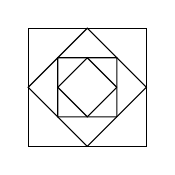
\begin{tikzpicture}
\pgfmathsetmacro{\k}{1.5}
\draw(0,0)--++(\k,0)coordinate[pos=0.5](a)--++(0,\k)coordinate[pos=0.5](b)--++(-\k,0)coordinate[pos=0.5](c)--++(0,-\k)coordinate[pos=0.5](d);
\draw(a)--(b)coordinate[pos=0.5](aa)--(c)coordinate[pos=0.5](bb)--(d)coordinate[pos=0.5](cc)--(a)coordinate[pos=0.5](dd);
\draw(aa)--(bb)coordinate[pos=0.5](aaa)--(cc)coordinate[pos=0.5](bbb)--(dd)coordinate[pos=0.5](ccc)--(aa)coordinate[pos=0.5](ddd);
\draw(aaa)--(bbb)coordinate[pos=0.5](aaaa)--(ccc)coordinate[pos=0.5](bbbb)--(ddd)coordinate[pos=0.5](cccc)--(aaa)coordinate[pos=0.5](dddd);
\end{tikzpicture}
\caption{چکور کے اندر چکور (سوال \حوالہ{سوال_تسلسل_چکور})}
\label{شکل_سوال_تسلسل_چکور}
\end{minipage}\hfill
\begin{minipage}{0.3\textwidth}
\centering
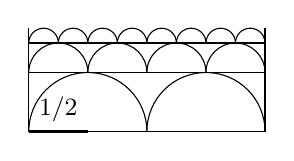
\begin{tikzpicture}[font=\small]
\pgfmathsetmacro{\k}{0.75}
\draw(0,\k+\k/2+\k/4)--(0,0)--(0,0)--(4*\k,0)--(4*\k,\k+\k/2+\k/4);
\draw(0,\k)--++(4*\k,0);
\draw(0,\k+\k/2)--++(4*\k,0);
\draw([shift={(0:\k)}]\k,0) arc (0:180:\k);
\draw([shift={(0:\k)}]3*\k,0) arc (0:180:\k);
\foreach \x in {1,3,5,7}{\draw([shift={(0:\k/2)}]\x*\k/2,\k) arc (0:180:\k/2);}
\foreach \x in {1,3,5,7,9,11,13,15}{\draw([shift={(0:\k/4)}]\x*\k/4,\k+\k/2) arc (0:180:\k/4);}
\draw[thick](0,0)--(\k,0)node[pos=0.5,above]{$1/2$};
\end{tikzpicture}
\caption{نصف دائروں کی قطاریں (سوال \حوالہ{سوال_تسلسل_نصف_دائرے})}
\label{شکل_سوال_تسلسل_نصف_دائرے}
\end{minipage}\hfill
\begin{minipage}{0.3\textwidth}
\centering
\begin{tikzpicture}[font=\scriptsize]
\pgfmathsetmacro{\k}{1.75}
\draw(\k+\k/2,\k/2)--++(0,\k/6+\k/7);
\draw(0,0) rectangle (2*\k,\k);
\draw(\k/2,0)node[below]{$1$}  (0,\k/2)node[left]{$1$} (\k+\k/4,0)node[below]{$\tfrac{1}{2}$} (\k+\k/2+\k/8,0)node[below]{$\tfrac{1}{4}$};
\draw(\k,0)--++(0,\k);
\draw[dashed](\k+\k/2,\k/4+\k/5+\k/6+\k/7)--(\k+\k/2,\k);
\draw[dashed](\k+\k/2+\k/4,\k/4)--(\k+\k/2+\k/4,\k);
\draw(\k,\k/2)--++(\k/2,0)--++(0,-\k/2);
\draw(\k+\k/3,\k/2)--++(0,\k/3)--++(-\k/3,0);
\draw(\k/2,\k/2)node[]{$1$};
\draw(\k+\k/4,\k/4)node[]{$\tfrac{1}{2^2}$};
\draw(\k+\k/6,\k/2+\k/6)node[]{$\tfrac{1}{3^2}$};
\draw(\k+\k/2+\k/4,0)--++(0,\k/4)--++(-\k/4,0);
\draw(\k+\k/2+\k/5,\k/4)--++(0,\k/5)--++(-\k/5,0);
\draw(\k+\k/2+\k/6,\k/4+\k/5)--++(0,\k/6)--++(-\k/6,0);
\draw(\k+\k/2+\k/7,\k/4+\k/5+\k/6)--++(0,\k/7)--++(-\k/7,0);
\draw(\k+\k/2+\k/8,\k/8)node[]{$\tfrac{1}{4^2}$};
\draw(\k+\k/2+\k/10,\k/4+\k/10)node[]{$\tfrac{1}{5^2}$};
\draw(\k+\k/2,\k/4+\k/5)node[pin=45:{$\tfrac{1}{6^2}$}]{};
\draw(\k+\k/2+\k/4+\k/8,0)node[below]{$\cdots$};
\draw(\k+\k/2+\k/4+\k/8,\k/2)node[]{$\cdots$};
\end{tikzpicture}
\caption{رقبوں کا مجموعہ \عددی{2} سے کم ہے (سوال \حوالہ{سوال_تسلسل_رقبہ_دو})}
\label{شکل_سوال_تسلسل_رقبہ_دو}
\end{minipage}
\end{figure}
%====================
\ابتدا{سوال}\شناخت{سوال_تسلسل_نصف_دائرے}
نصف دائروں کی صفوں کو شکل \حوالہ{شکل_سوال_تسلسل_نصف_دائرے} میں دکھایا گیا ہے جہاں نچلی صف میں رداس \عددی{\tfrac{1}{2}} ہے۔ \عددی{n} ویں صف میں نصف دائروں کی تعداد \عددی{2^n}  اور رداس \عددی{1/2^n} ہو گا۔ تمام نصف دائروں کے رقبوں کا مجموعہ تلاش کریں۔
\انتہا{سوال}
%=========================
\ابتدا{سوال}
متناہی رقبہ گھیرنے والی ہلگے ون کوچ برفانی روئی (صفحہ\حوالہصفحہ{حصہ_تفرق_برف_کی_روئی})  کی لمبائی لامتناہی ہوتی ہے۔ اس حقیقت کو سمجھنے کی خاطر فرض کریں ہم ضلع \عددی{1} کی مساوی الاضلاع مثلث سے شروع کرتے ہیں۔
\begin{enumerate}[a.]
\item
\عددی{n} ویں منحنی \عددی{C_n} کی لمبائی \عددی{L_n} تلاش کر کے دکھائیں کہ \عددی{\lim_{n\to \infty}L_n=\infty}  ہو گا۔
\item
\عددی{C_n} کا رقبہ \عددی{S_n} تلاش کر کے \عددی{\lim_{n\to\infty}S_n} معلوم کریں۔
\end{enumerate}
جواب:\quad
(الف) \عددی{3(\tfrac{4}{3})^{n-1}}، (ب) \عددی{A_n=A+\tfrac{1}{3}A+\tfrac{1}{3}(\tfrac{4}{9})A+\cdots+\tfrac{1}{3}(\tfrac{4}{9})^{n-2}A}،\\
  \عددی{\lim_{n\to\infty}A_n=\tfrac{2\sqrt{3}}{5}}
\انتہا{سوال}
%=========================
\ابتدا{سوال}\شناخت{سوال_تسلسل_رقبہ_دو}
ہم اس حقیقت کی غیر رسمی ثبوت کہ \عددی{\sum_{n=1}^{\infty}\tfrac{1}{n^2}} کی قیمت \عددی{2} سے کم ہے شکل \حوالہ{شکل_سوال_تسلسل_رقبہ_دو} کی مدد سے پیش کرتے ہیں۔ آپ کو کیا نظر آتا ہے؟
\انتہا{سوال}
%========================

\حصہ{غیر منفی اجزاء والے تسلسل کا تکملی پرکھ}
ہم تسلسل \عددی{\sum a_n} کے بارے میں دو سوالات کرتے ہیں:
\begin{enumerate}[a.]
\item
کیا یہ تسلسل مرتکز ہے؟
\item
اگر تسلسل مرتکز ہو تب اس کا مجموعہ کیا ہے؟
\end{enumerate}

اس باب کا باقی بیشتر حصہ پہلے سوال کا جواب دے گا۔ حقیقتاً دوسرا سوال بھی اتنا ہی اہم ہے اور ہم اس پر بعد میں غور کریں گے۔

اس حصہ میں اور اگلے دو حصوں میں ایسے تسلسل پر غور کیا جائے گا جن میں منفی اجزاء نہیں پائے جاتے ہوں۔ اس شرط کی بنا ان تسلسل کے جزوی مجموعے غیر گھٹتے ترتیبات دیتے ہیں اور وہ غیر گھٹتے ترتیبات جو  اوپر سے محدود ہوں ہر صورت مرتکز ہوتے ہیں (مسئلہ \حوالہ{مسئلہ_تسلسل_غیر_گھٹتا_تسلسل})۔ یہ دکھانے کی خاطر کہ ایک غیر منفی اجزاء والا تسلسل مرتکز ہے، ہمیں صرف اتنا دکھانا ہو گا کہ اس تسلسل کے جزوی مجموعے اوپر سے محدود ہیں۔

ابتدا میں یوں معلوم ہوتا ہے جیسے اس ترکیب سے ارتکاز کی تصدیق کرنے کے باوجود تسلسل کا مجموعہ نہ جاننا ایک عیب ہے۔ کیا بہتر ہوتا کہ ہم جزوی مجموعوں کے کلیات سے تسلسل کا مجموعہ بلا واسطہ تلاش کرتے۔ حقیقت میں ہمیں عموماً جزوی مجموعوں کے کلیات معلوم نہیں ہوں گے  اور اسی بنا ہمیں دو قدمی طریقہ کار استعمال کرنا ہو گا جہاں پہلے قدم میں تسلسل کا ارتکاز جانا جاتا ہے اور دوسرے قدم میں مجموعے کی تخمینی قیمت تلاش کی جاتی ہے۔ 

\جزوحصہء{غیر گھٹتے جزوی مجموعے}
فرض کریں کہ تمام \عددی{n} کے لئے \عددی{a_n\ge 0} ہو اور \عددی{\sum_{n=1}^{\infty}a_n} لامتناہی تسلسل ہو۔
 تب چونکہ \عددی{s_{n+1}=s_n+a_n} ہے لہٰذا ہر جزوی مجموعہ گزشتہ جزوی مجموعے سے بڑا یا اس کے برابر ہو گا:
\begin{align*}
s_1\le s_2\le s_3\le \cdots\le s_n\le s_{n+1}\le \cdots
\end{align*}
اب جزوی مجموعے غیر گھٹتا ترتیب بناتے ہیں اور مسئلہ \حوالہ{مسئلہ_تسلسل_غیر_گھٹتا_تسلسل} کے تحت یہ تسلسل صرف اور صرف اس صورت مرتکز ہو گا جب اس کے جزوی مجموعات اوپر سے محدود ہوں۔

\ابتدا{ضمنی نتیجہ}\شناخت{ضمنی_تسلسل_نتیجہ_الف} برائے مسئلہ \حوالہ{مسئلہ_تسلسل_غیر_گھٹتا_تسلسل}
غیر منفی اجزاء کا تسلسل \عددی{\sum_{n=1}^{\infty}a_n} صرف اور صرف اس صورت مرتکز ہو گا جب اس کے جزوی مجموعات اوپر سے محدود ہوں۔
\انتہا{ضمنی نتیجہ}
%=========================

\ابتدا{مثال}\ترچھا{ہارمونی تسلسل}\\
درج ذیل تسلسل کو \اصطلاح{ہارمونی تسلسل}\فرہنگ{تسلسل!ہارمونی}\حاشیہب{harmonic series}\فرہنگ{series!harmonic} کہتے ہیں۔
\begin{align*}
\sum_{n=1}^{\infty}\frac{1}{n}=1+\frac{1}{2}+\frac{1}{3}+\cdots+\frac{1}{n}+\cdots
\end{align*}
اس کے جزوی مجموعوں کی کوئی بالائی حد بندی نہیں پائی جاتی ہے لہٰذا یہ  مرتکز  تسلسل ہے۔ اس حقیقت کو جاننے کی خاطر ہم اجزاء کے گروہ بناتے ہیں۔
\begin{align*}
1+\frac{1}{2}+\underbrace{\big(\frac{1}{3}+\frac{1}{4}\big)}_{>\tfrac{2}{4}=\tfrac{1}{2}}+\underbrace{\big(\frac{1}{5}+\frac{1}{6}+\frac{1}{7}+\frac{1}{8}\big)}_{>\tfrac{4}{8}=\tfrac{1}{2}}+\underbrace{\big(\frac{1}{9}+\frac{1}{10}+\cdots+\frac{1}{16}\big)}_{>\tfrac{8}{16}=\tfrac{1}{2}}+\cdots
\end{align*}
پہلے دو اجزاء کا مجموعہ \عددی{1.5} ہے۔اگلے دو اجزاء کا مجموعہ \عددی{\tfrac{1}{3}+\tfrac{1}{4}} ہے جو \عددی{\tfrac{1}{4}+\tfrac{1}{4}=\tfrac{1}{2}} سے بڑا ہے۔ اگلے چار اجزاء کا مجموعہ \عددی{\tfrac{1}{5}+\tfrac{1}{6}+\tfrac{1}{7}+\tfrac{1}{8}} ہے جو \عددی{\tfrac{1}{8}+\tfrac{1}{8}+\tfrac{1}{8}+\tfrac{1}{8}=\tfrac{1}{2}} سے بڑا ہے۔ اگلے آٹھ اجزاء کا مجموعہ
 \عددی{\tfrac{1}{9}+\tfrac{1}{10}+\tfrac{1}{11}+\tfrac{1}{12}+\tfrac{1}{13}+\tfrac{1}{14}+\tfrac{1}{15}+\tfrac{1}{16}} ہے جو  \عددی{\tfrac{1}{16}+\tfrac{1}{16}+\tfrac{1}{16}+\tfrac{1}{16}+\tfrac{1}{16}+\tfrac{1}{16}+\tfrac{1}{16}+\tfrac{1}{16}=\tfrac{1}{2}} سے بڑا ہے۔ اسی طرح اگلے سولہ اجزاء کا مجموعہ بھی \عددی{\tfrac{1}{2}} سے بڑا ہو گا، وغیرہ وغیرہ۔ یوں جزو \عددی{\tfrac{1}{2^{n+1}}} پر اختتام پذیر  \عددی{2^n} اجزاء کا مجموعہ \عددی{\tfrac{2^n}{2^{n+1}}=\tfrac{1}{2}} سے بڑا ہو گا۔جزوی مجموعات کی ترتیب اوپر سے محدود نہیں ہے: اگر \عددی{n=2^k} ہو تب جزوی مجموعہ \عددی{s_n} کی قیمت \عددی{\tfrac{k}{2}} سے بڑی ہو گی۔ ہارمونی تسلسل منفرج ہے۔
\انتہا{مثال}
%===========================

دھیان رہے کہ ہارمونی تسلسل کا \عددی{n} واں جزو \عددی{\tfrac{1}{n}} ہے جو \عددی{0} پر مرتکز ہے لیکن ہارمونی تسلسل منفرج ہے۔یوں ہارمونی تسلسل کے انفراج کو دریافت کرنے میں انفراج کا \عددی{n} ویں جزو پرکھ  نا کام  ہوتا ہے۔

\جزوحصہء{تکملی پرکھ}
ہم ہارمونی تسلسل سے تعلق رکھنے والے ایک تسلسل، جس کا \عددی{n} واں جزو \عددی{\tfrac{1}{n^2}} ہے، کو استعمال کرتے ہوئے تکملی پرکھ کو متعارف کرتے ہیں۔

\ابتدا{مثال}\شناخت{مثال_تسلسل_مرتکز_تسلسل_موازنہ_تکمل}
کیا درج ذیل تسلسل مرتکز ہے؟
\begin{align*}
\sum_{n=1}^{\infty}\frac{1}{n^2}=1+\frac{1}{4}+\frac{1}{9}+\frac{1}{16}+\cdots+\frac{1}{n^2}+\cdots
\end{align*}
حل:\quad
ہم \عددی{\int_1^{\infty}\tfrac{\dif x}{x^2}} کے ساتھ موازنہ کرتے ہوئے \عددی{\sum_{n=1}^{\infty}\tfrac{1}{n^2}} کی ارتکاز دریافت کرتے ہیں۔ موازنہ کرنے کی خاطر ہم تسلسل کے اجزاء کو تفاعل \عددی{f(x)=\tfrac{1}{x^2}} کی قیمتیں تصور کرتے ہیں اور ان قیمتوں کو منحنی \عددی{y=\tfrac{1}{x^2}} کے نیچے مستطیل رقبے تصور کرتے ہیں۔

جیسا شکل \حوالہ{شکل_مثال_تسلسل_مرتکز_تسلسل_موازنہ_تکمل} میں دکھایا گیا ہے درج ذیل ہو گا۔
\begin{align*}
s_n&=\frac{1}{1^2}+\frac{1}{2^2}+\frac{1}{3^2}+\cdots+\frac{1}{n^2}\\
&=f(1)+f(2)+f(3)+\cdots+f(n)\\
&<f(1)+\int_1^{n}\frac{1}{x^2}\dif x\\
&<1+\int_1^{\infty}\frac{1}{x^2}\dif x\\
&<1+1=2&&\text{\RL{(مثال \حوالہ{مثال_طریقہ_منحنی_کے_نیچے_رقبہ_متناہی_یا_نہیں})}}
\end{align*}
یوں \عددی{\sum_{n=1}^{\infty}\tfrac{1}{n^2}} کے جزوی مجموعات اوپر سے (\عددی{2} تک) محدود ہیں لہٰذا یہ تسلسل مرتکز ہو گا۔  اس تسلسل کا مجموعہ درحقیقت \عددی{\tfrac{\pi^2}{6}\approx 1.64493} ہے۔
\انتہا{مثال}
%=======================
\begin{figure}
\centering
\begin{tikzpicture}[font=\small,declare function={f(\x)=1/(\x^2);}]
\begin{axis}[clip=false,small,axis lines=middle,xlabel={$x$},ylabel={$y$},xlabel style={at={(current axis.right of origin)},anchor=west},ylabel style={at={(current axis.above origin)},anchor=south},xmin=0,ymin=0,ytick={\empty},xtick={1,2,3,4,7,8},xticklabels={$1$,$2$,$3$,$4$,$n-1$,$n$}]
\addplot[smooth,domain=0.9:9]{f(x)};
\draw(0,{f(1)})--(1,{f(1)})node[right]{$(1,f(1))$}--(1,0);
\draw(1,{f(2)})--(2,{f(2)})node[pin={[pin distance=1cm]70:{$(2,f(2))$}}]{}--(2,0);
\draw(2,{f(3)})--(3,{f(3)})node[pin={[pin distance=1cm]50:{$(3,f(3))$}}]{}--(3,0);
\draw(3,{f(4)})--(4,{f(4)})--(4,0);
\draw(1/2,{1/2*f(1)})node[]{$\tfrac{1}{1^2}$};
\draw(1+1/2,{1/2*f(2)})node[]{$\tfrac{1}{2^2}$};
\draw(2.2,{1/3*f(3)})node[pin=60:{$\tfrac{1}{3^2}$}]{};
\draw(3.2,{1/4*f(4)})node[pin=30:{$\tfrac{1}{4^2}$}]{};
\draw(8,{f(8)})node[pin=45:{$(n,f(n))$}]{};
\draw(7.5,{0})node[pin=70:{$\tfrac{1}{n^2}$}]{};
\draw(7,{f(1)})node[]{$f(x)=\frac{1}{x^2}$};
\end{axis}
\end{tikzpicture}
\caption{رقبہ کا موازنہ (مثال \حوالہ{مثال_تسلسل_مرتکز_تسلسل_موازنہ_تکمل})}
\label{شکل_مثال_تسلسل_مرتکز_تسلسل_موازنہ_تکمل}
\end{figure}

\ابتدا{پرکھ}\موٹا{تکملی پرکھ}\\
فرض کریں \عددی{\{a_n\}} مثبت اجزاء کی ترتیب ہے۔ مزید فرض کریں کہ \عددی{a_n=f(n)} ہے جہاں تمام \عددی{x\ge N} کے لئے ( \عددی{N} مثبت عدد صحیح ہے)  متغیر \عددی{x} کا \عددی{f}  استمراری، مثبت اور گھٹتا تفاعل ہے۔ تب تسلسل \عددی{\sum_{n=N}^{\infty}a_n} اور تکمل \عددی{\int_N^{\infty}f(x)\dif  x} دونوں مرتکز یا دونوں منفرج ہوں گے۔
\انتہا{پرکھ}
%==================
\ابتدا{ثبوت پرکھ}
ہم \عددی{N=1} کے لئے پہلے اس پرکھ کو ثابت کرتے ہیں۔ عمومی \عددی{N} کے لئے ثبوت اسی طرح کا ہے۔ 

ہم اس مفروضہ سے شروع کرتے ہیں کہ تمام \عددی{n} کے لئے \عددی{f} گھٹتا تفاعل  اور \عددی{f(n)=a_n} ہیں۔ یوں شکل \حوالہ{شکل_تسلسل_تکملی_پرکھ_ثبوت}-الف میں وہ مستطیل جن کے رقبے \عددی{a_1,a_2,\cdots,a_n}  ہیں کا مجموعی رقبہ، \عددی{x=1} تا \عددی{x=n+1} ترسیم \عددی{y=f(x)} کے نیچے رقبہ سے زیادہ ہے یعنی:
\begin{align*}
\int_1^{n+1}f(x)\dif x\le a_1+a_2+\cdots+a_n
\end{align*} 
شکل \حوالہ{شکل_تسلسل_تکملی_پرکھ_ثبوت}-ب میں مستطیلوں کو ہر نقطہ کے بائیں جانب بنایا گیا ہے۔ اگر ہم وقتی طور پر پہلی مستطیل، جس کا رقبہ \عددی{a_1} ہے، کو نظر انداز کریں تب درج ذیل ہو گا۔
\begin{align*}
a_2+a_3+\cdots+a_n\le \int_1^nf(x)\dif x
\end{align*}
اگر ہم \عددی{a_1} کو بھی شامل کریں تب درج ذیل لکھا جا سکتا ہے۔
\begin{align*}
a_1+a_2+a_3+\cdots+a_n\le a_1+\int_1^nf(x)\dif x
\end{align*}
ان نتائج سے 
\begin{align}\label{مساوات_تسلسل_عدم_مساواتیں}
\int_1^{n+1}f(x)\dif x\le a_1+a_2+\cdots+a_n\le  a_1+\int_1^nf(x)\dif x
\end{align}
حاصل ہوتا ہے۔ اگر \عددی{\int_1^{\infty}f(x)\dif x} متناہی ہو تب دائیں عدم مساوات کے تحت \عددی{\sum a_n} متناہی ہو گا۔  اگر \عددی{\int_1^{\infty}f(x)\dif x} لامتناہی ہو تب بائیں عدم مساوات کے تحت \عددی{\sum a_n} لامتناہی ہو گا۔ 

یوں تسلسل اور تکمل دونوں مرتکز یا دونوں منفرج ہوں گے۔
\انتہا{ثبوت پرکھ}
%=======================
\begin{figure}
\centering
\begin{subfigure}{0.45\textwidth}
\centering
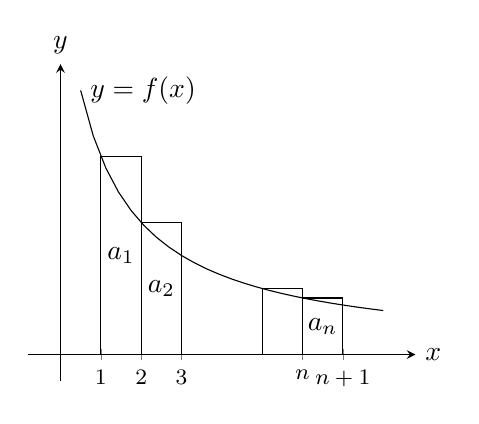
\begin{tikzpicture}[declare function={f(\x)=1/(1+\x);}]
\begin{axis}[small,axis lines=middle,xlabel={$x$},ylabel={$y$},xmin=0,ymin=0,enlargelimits=true,xtick={1,2,3,6,7},xticklabels={$1$,$2$,$3$,$n$,$n+1$},ytick={\empty},xlabel style={at={(current axis.right of origin)},anchor=west},ylabel style={at={(current axis.above origin)},anchor=south}]
\addplot[domain=0.5:8]{f(x)}node[pos=0,right]{$y=f(x)$};
\draw(1,0)--(1,{f(1)})--(2,{f(1)})--(2,{f(2)});
\draw(2,0)--(2,{f(2)})--(3,{f(2)})--(3,0);
\draw(5,0)--(5,{f(5)})--(6,{f(5)})--(6,{f(6)});
\draw(6,0)--(6,{f(6)})--(7,{f(6)})--(7,0);
\draw(1.5,{1/2*f(1)})node[]{$a_1$};
\draw(2.5,{1/2*f(2)})node[]{$a_2$};
\draw(6.5,{1/2*f(6)})node[]{$a_n$};
\end{axis}
\end{tikzpicture}
\caption{}
\end{subfigure}\hfill
\begin{subfigure}{0.45\textwidth}
\centering
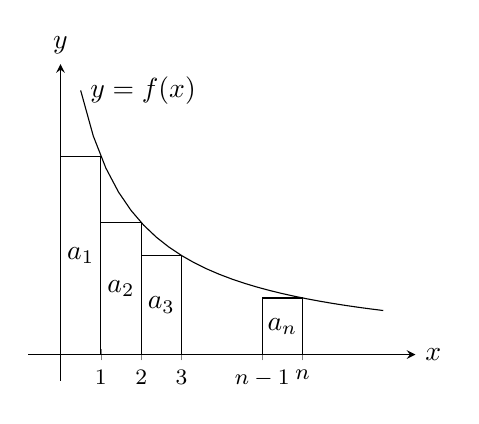
\begin{tikzpicture}[declare function={f(\x)=1/(1+\x);}]
\begin{axis}[small,axis lines=middle,xlabel={$x$},ylabel={$y$},xmin=0,ymin=0,enlargelimits=true,xtick={1,2,3,5,6},xticklabels={$1$,$2$,$3$,$n-1$,$n$},ytick={\empty},xlabel style={at={(current axis.right of origin)},anchor=west},ylabel style={at={(current axis.above origin)},anchor=south}]
\addplot[domain=0.5:8]{f(x)}node[pos=0,right]{$y=f(x)$};
\draw(0,{f(1)})--(1,{f(1)})--(1,0);
\draw(1,{f(2)})--(2,{f(2)})--(2,0);
\draw(2,{f(3)})--(3,{f(3)})--(3,0);
\draw(5,0)--(5,{f(6)})--(6,{f(6)})--(6,0);
\draw(0.5,{1/2*f(1)})node[]{$a_1$};
\draw(1.5,{1/2*f(2)})node[]{$a_2$};
\draw(2.5,{1/2*f(3)})node[]{$a_3$};
\draw(5.5,{1/2*f(6)})node[]{$a_n$};
\end{axis}
\end{tikzpicture}
\caption{}
\end{subfigure}
\caption{تکملی پرکھ کے تحت تسلسل $\sum_{n=1}^{\infty}a_n$ اور تکمل $\int_1^{\infty}f(x)\dif x$ دونوں مرتکز یا دونوں منفرج ہوں گے۔}
\label{شکل_تسلسل_تکملی_پرکھ_ثبوت}
\end{figure}

%====================
دھیان رہے کہ ارتکاز کی صورت میں تکمل اور تسلسل کی قیمتیں مختلف ہو سکتی ہیں جیسا مثال \حوالہ{مثال_تسلسل_مرتکز_تسلسل_موازنہ_تکمل} میں دیکھا گیا جہاں \عددی{\sum_{n=1}^{\infty}\tfrac{1}{n^2}=\tfrac{\pi^2}{6}} اور \عددی{\int_1^{\infty}\tfrac{1}{x^2}\dif x=1} تھے۔

\ابتدا{مثال}
دکھائیں کہ \عددی{p} تسلسل
\begin{align}
\sum_{n=1}^{\infty}\frac{1}{n^p}=\frac{1}{1^p}+\frac{1}{2^p}+\frac{1}{3^p}+\cdots+\frac{1}{n^p}+\cdots
\end{align}
جہاں \عددی{p} حقیقی مستقل ہے، \عددی{p>1} کی صورت میں مرتکز جبکہ \عددی{p\le 1} کی صورت میں منفرج ہو گا۔

حل:\quad
اگر \عددی{p>1} ہو تب \عددی{f(x)=\tfrac{1}{x^p}} متغیر \عددی{x} کا مثبت گھٹتا تفاعل ہو گا۔ اب چونکہ
\begin{align*}
\int_1^{\infty}\frac{1}{x^p}\dif x&=\int_1^{\infty}x^{-p}\dif x=\lim_{b\to\infty}\big[\frac{x^{-p+1}}{-p+1}\big]_1^b\\
&=\frac{1}{1-p}\lim_{b\to\infty}(\frac{1}{b^{p-1}}-1)\\
&=\frac{1}{1-p}(0-1)=\frac{1}{p-1}
\end{align*}
ہے لہٰذا تکملی پرکھ کے تحت یہ تسلسل مرتکز ہو گا۔

اگر \عددی{p<1}ہو تب \عددی{1-p>0} ہو گا لہٰذا درج ذیل لکھا جا سکتا ہے۔
\begin{align*}
\int_1^{\infty}\frac{1}{x^p}\dif x=\frac{1}{1-p}\lim_{b\to\infty}(b^{1-p}-1)=\infty
\end{align*}
تکملی پرکھ کے تحت یہ تسلسل منفرج ہو گا۔

اگر \عددی{p=1} ہو تب درج ذیل منفرج (ہارمونی) تسلسل پایا جائے گا۔
\begin{align*}
1+\frac{1}{2}+\frac{1}{3}+\cdots+\frac{1}{n}+\cdots
\end{align*} 
یوں \عددی{p>1} لے ارتکاز  لیکن \عددی{p<1} اور \عددی{p=0} کے لئے انفراج پایا جاتا ہے۔
\انتہا{مثال}
%=====================
\حصہء{سوالات}
\موٹا{ارتکاز اور انفراج کی معلومات}\\
سوال \حوالہ{سوال_تسلسل_ارتکاز_یا_انفراج_الف} تا سوال \حوالہ{سوال_تسلسل_ارتکاز_یا_انفراج_ب} میں کون سا تسلسل مرتکز اور کان سا تسلسل منفرج ہے؟ اپنے جواب کی وجہ پیش کریں۔(جوابات دیکھتے ہوئے یاد رہے کہ تسلسل کی ارتکاز یا انفراج جاننے کے کئی طریقے ہو سکتے ہیں)

\ابتدا{سوال}\شناخت{سوال_تسلسل_ارتکاز_یا_انفراج_الف}
$\sum\limits_{n=1}^{\infty}\frac{1}{10^n}$\\
جواب:\quad
مرتکز؛ ہندسی تسلسل، \عددی{r=\tfrac{1}{10}<1}
\انتہا{سوال}
%==========================
\ابتدا{سوال}
$\sum\limits_{n=1}^{\infty}e^{-n}$
\انتہا{سوال}
%==========================
\ابتدا{سوال}
$\sum\limits_{n=1}^{\infty}\frac{n}{n+1}$\\
جواب:\quad
منفرج؛ \عددی{\lim_{n\to\infty}\tfrac{n}{n+1}=1\ne 0} 
\انتہا{سوال}
%==========================
\ابتدا{سوال}
$\sum\limits_{n=1}^{\infty}\frac{5}{n+1}$
\انتہا{سوال}
%==========================
\ابتدا{سوال}
$\sum\limits_{n=1}^{\infty}\frac{3}{\sqrt{n}}$\\
جواب:\quad
منفرج؛ \عددی{p} تسلسل، \عددی{p<1}
\انتہا{سوال}
%==========================
\ابتدا{سوال}
$\sum\limits_{n=1}^{\infty}\frac{-2}{n\sqrt{n}}$
\انتہا{سوال}
%==========================
\ابتدا{سوال}
$\sum\limits_{n=1}^{\infty}-\frac{1}{8^n}$\\
جواب:\quad
مرتکز؛ ہندسی تسلسل، \عددی{r=\tfrac{1}{8}<1}
\انتہا{سوال}
%==========================
\ابتدا{سوال}
$\sum\limits_{n=1}^{\infty}-\frac{8}{n}$
\انتہا{سوال}
%==========================
\ابتدا{سوال}
$\sum\limits_{n=2}^{\infty}\frac{\ln n}{n}$\\
جواب:\quad
منفرج؛ تکملی پرکھ
\انتہا{سوال}
%==========================
\ابتدا{سوال}
$\sum\limits_{n=2}^{\infty}\frac{\ln n}{\sqrt{n}}$
\انتہا{سوال}
%==========================
\ابتدا{سوال}
$\sum\limits_{n=1}^{\infty}\frac{2^n}{3^n}$\\
جواب:\quad
مرتکز؛ ہندسی تسلسل، \عددی{r=\tfrac{2}{3}<1}
\انتہا{سوال}
%==========================
\ابتدا{سوال}
$\sum\limits_{n=1}^{\infty}\frac{5^n}{4^n+3}$
\انتہا{سوال}
%==========================
\ابتدا{سوال}
$\sum\limits_{n=0}^{\infty}\frac{-2}{n+1}$\\
جواب:\quad
منفرج؛ تکملی پرکھ
\انتہا{سوال}
%==========================
\ابتدا{سوال}
$\sum\limits_{n=1}^{\infty}\frac{1}{2n-1}$
\انتہا{سوال}
%==========================
\ابتدا{سوال}
$\sum\limits_{n=1}^{\infty}\frac{2^n}{n+1}$\\
جواب:\quad
منفرج؛ \عددی{\lim_{n\to\infty}\tfrac{2^n}{n+1}\ne 0}
\انتہا{سوال}
%==========================
\ابتدا{سوال}
$\sum\limits_{n=1}^{\infty}\frac{1}{\sqrt{n}(\sqrt{n}+1)}$
\انتہا{سوال}
%==========================
\ابتدا{سوال}
$\sum\limits_{n=2}^{\infty}\frac{\sqrt{n}}{\ln n}$\\
جواب:\quad
منفرج؛ \عددی{\lim_{n\to\infty}(\tfrac{\sqrt{n}}{\ln n})\ne 0}
\انتہا{سوال}
%==========================
\ابتدا{سوال}
$\sum\limits_{n=1}^{\infty}\big(1+\frac{1}{n}\big)^n$
\انتہا{سوال}
%==========================
\ابتدا{سوال}
$\sum\limits_{n=1}^{\infty}\frac{1}{(\ln 2)^n}$\\
جواب:\quad
منفرج؛ ہندسی تسلسل، \عددی{r=\tfrac{1}{\ln2}>1}
\انتہا{سوال}
%==========================
\ابتدا{سوال}
$\sum\limits_{n=1}^{\infty}\frac{1}{(\ln 3)^n}$
\انتہا{سوال}
%==========================
\ابتدا{سوال}
$\sum\limits_{n=3}^{\infty}\frac{1/n}{(\ln n)\sqrt{\ln^2 n-1}}$\\
جواب:\quad
مرتکز؛  تکملی پرکھ
\انتہا{سوال}
%==========================
\ابتدا{سوال}
$\sum\limits_{n=1}^{\infty}\frac{1}{n(1+\ln^2n)}$
\انتہا{سوال}
%==========================
\ابتدا{سوال}
$\sum\limits_{n=1}^{\infty}n\sin\frac{1}{n}$\\
جواب:\quad
منفرج؛ \عددی{n} واں جزو پرکھ
\انتہا{سوال}
%==========================
\ابتدا{سوال}
$\sum\limits_{n=1}^{\infty}n\tan \frac{1}{n}$
\انتہا{سوال}
%==========================
\ابتدا{سوال}
$\sum\limits_{n=1}^{\infty}\frac{e^n}{1+e^{2n}}$\\
جواب:\quad
مرتکز؛ تکملی پرکھ
\انتہا{سوال}
%==========================
\ابتدا{سوال}
$\sum\limits_{n=1}^{\infty}\frac{2}{1+e^n}$
\انتہا{سوال}
%==========================
\ابتدا{سوال}
$\sum\limits_{n=1}^{\infty}\frac{8\tan^{-1}n}{1+n^2}$\\
جواب:\quad
مرتکز؛ تکملی پرکھ
\انتہا{سوال}
%==========================
\ابتدا{سوال}
$\sum\limits_{n=1}^{\infty}\frac{n}{n^2+1}$
\انتہا{سوال}
%==========================
\ابتدا{سوال}
$\sum\limits_{n=1}^{\infty}\sech n$\\
جواب:\quad
مرتکز؛ تکملی پرکھ
\انتہا{سوال}
%==========================
\ابتدا{سوال}\شناخت{سوال_تسلسل_ارتکاز_یا_انفراج_ب}
$\sum\limits_{n=1}^{\infty}\sech^2 n$
\انتہا{سوال}
%==========================
\موٹا{نظریہ اور مثالیں}\\
سوال \حوالہ{سوال_تسلسل_ارتکاز_کا_اے_الف} اور سوال \حوالہ{سوال_تسلسل_ارتکاز_کا_اے_ب} میں اگر کسی \عددی{a} کے لئے تسلسل مرتکز ہو تب \عددی{a} تلاش کریں۔ 

\ابتدا{سوال}\شناخت{سوال_تسلسل_ارتکاز_کا_اے_الف}
$\sum\limits_{n=1}^{\infty}\big(\frac{a}{n+2}-\frac{1}{n+4}\big)$\\
جواب:\quad
(الف) \عددی{a=1}
\انتہا{سوال}
%========================
\ابتدا{سوال}\شناخت{سوال_تسلسل_ارتکاز_کا_اے_ب}
$\sum\limits_{n=3}^{\infty}\big(\frac{1}{n-1}-\frac{2a}{n+1}\big)$
\انتہا{سوال}
%========================
\ابتدا{سوال}
\begin{enumerate}[a.]
\item
شکل \حوالہ{شکل_مثال_تسلسل_مرتکز_تسلسل_موازنہ_تکمل} اور شکل \حوالہ{شکل_تسلسل_تکملی_پرکھ_ثبوت} کی طرز کے اشکال بنا کر دکھائیں کہ ہارمونی تسلسل کے جزوی مجموعات درج ذیل عدم مساواتوں کو مطمئن کرتے ہیں۔ 
\begin{align*}
\ln(n+1)&=\int_1^{n+1}\frac{1}{x}\dif x\le 1+\frac{1}{2}+\cdots+\frac{1}{n}\\
&\le 1+\int_1^n\frac{1}{x}\dif x=1+\ln n
\end{align*}
%
\item
ہارمونی تسلسل کی انفراج  تجرباتی طور نظر نہیں آتی ہے اگرچہ ہم جانتے ہیں کہ یہ تسلسل منفرج ہے۔ بس اس کے جزوی مجموعات بہت آہستہ بڑھتے ہیں۔یہ دیکھنے کی خاطر فرض کریں ہم \عددی{s_1=1} سے شروع کر کے ہر سیکنڈ ہارمونی تسلسل میں ایک جزو شامل کرتے ہیں۔کائنات کی ابتدا سے شروع کرتے ہوئے اب تک (تقریباً \عددی{13} ارب سال بعد) شامل اجزاء کا جزوی مجموعہ کیا ہو گا؟ (ایک سال میں \عددی{365} دن لیں۔)
\end{enumerate}
جواب:\quad
(ب) تقریباً \عددی{41.55}
\انتہا{سوال}
%==============
\ابتدا{سوال}
کیا \عددی{x} کی کسی قیمت کے لئے \عددی{\sum_{n=1}^{\infty}\tfrac{1}{nx}} مرتکز ہو گا؟ اپنے جواب کی وجہ پیش کریں۔
\انتہا{سوال}
%============================
\ابتدا{سوال}\شناخت{سوال_تسلسل_چھوٹا_منفرج_الف}
کیا یہ درست ہے کہ اگر \عددی{\sum_{n=1}^{\infty}a_n} مثبت اعداد کا منفرج تسلسل ہو تب تمام \عددی{n} کے لئے \عددی{b_n<a_n} کی صورت میں مثبت اعداد کا ایک تسلسل \عددی{\sum_{n=1}^{\infty}b_n} بھی منفرج ہو گا؟ کیا مثبت اعداد کا  "چھوٹے سے چھوٹا" منفرج تسلسل پایا جاتا ہے؟ اپنے جواب کی وجہ پیش کریں۔\\
جواب:\quad
درست ہے۔
\انتہا{سوال}
%=========================
\ابتدا{سوال}
کیا مثبت اعداد کا "بڑے سے بڑا" منفرج تسلسل پایا جاتا ہے (سوال \حوالہ{سوال_تسلسل_چھوٹا_منفرج_الف})؟
\انتہا{سوال}
%==========================
\ابتدا{سوال}\شناخت{سوال_تسلسل_کوشی_پرکھ_جمود}\ترچھا{کوشی پرکھ جمود}\\
کوشی پرکھ جمود کہتا ہے: فرض کریں \عددی{\{a_n\}} مثبت اجزاء کی غیر گھٹتی ترتیب ہے  (تمام \عددی{n} کے لئے \عددی{a_n\ge a_{n+1}})  جو \عددی{0} پر مرتکز ہے۔تب \عددی{\sum a_n} صرف اور صرف اس صورت مرتکز ہو گا جب \عددی{\sum 2^n a_{2^n}} مرتکز ہو۔ مثال کے طور پر \عددی{\sum \tfrac{1}{n}}  اس لئے منفرج  ہے کہ \عددی{\sum 2^n\cdot (\tfrac{1}{2^n})=\sum 1} منفرج ہے۔ دکھائیں کہ یہ پرکھ کیوں کام کرتا ہے۔
\انتہا{سوال}
%======================
\ابتدا{سوال}\شناخت{سوال_کوشی_پرکھ_جمود_کی_مدد}
کوشی پرکھ جمود (سوال \حوالہ{سوال_تسلسل_کوشی_پرکھ_جمود}) استعمال کرتے ہوئے دکھائیں کہ
\begin{enumerate}[a.]
\item
\عددی{\sum\limits_{n=2}^{\infty}\frac{1}{n\ln n}} منفرج ہے۔
\item
\عددی{p>1} کے لئے \عددی{\sum\limits_{n=1}^{\infty}\tfrac{1}{n^p}} مرتکز اور \عددی{p\le 1} کے لئے منفرج ہے۔
\end{enumerate}
\انتہا{سوال}
%=====================
\ابتدا{سوال}\شناخت{سوال_تسلسل_لوگارتھمی_پی_تسلسل}\ترچھا{لوگارتھمی \عددی{p} تسلسل}\\
\begin{enumerate}[a.]
\item
دکھائیں کہ صرف اور صرف \عددی{p>1} کے لئے  \عددی{\int_2^{\infty}\tfrac{\dif x}{x(\ln x)^p}} مرتکز ہو گا۔
\item
تسلسل \عددی{\sum_2^{\infty}\tfrac{1}{n(\ln n)^p}} کی ارتکاز پر جزو-الف کا کیا اثر ہو گا؟ اپنے جواب کی وجہ پیش کریں۔
\end{enumerate}
\انتہا{سوال}
%=====================
\ابتدا{سوال}
درج ذیل میں کون سے تسلسل مرتکز اور کون سے منفرج ہیں۔ سوال \حوالہ{سوال_تسلسل_لوگارتھمی_پی_تسلسل} کے نتائج بروئے کار لائیں۔ اپنے جواب کی وجہ پیش کریں۔
\begin{multicols}{4}
\begin{enumerate}[a.]
\item
$\sum\limits_{n=2}^{\infty}\frac{1}{n\ln n}$
\item
$\sum\limits_{n=2}^{\infty}\frac{1}{n(\ln n)^{1.01}}$
\item
$\sum\limits_{n=2}^{\infty}\frac{1}{n\ln (n^3)}$
\item
$\sum\limits_{n=2}^{\infty}\frac{1}{n(\ln n)^3}$
\end{enumerate}
\end{multicols}
\انتہا{سوال}
%======================
\ابتدا{سوال}\ترچھا{یولر مستقل}\\
ہم شکل \حوالہ{شکل_تسلسل_تکملی_پرکھ_ثبوت} کی طرح اشکال کو دیکھ کر ہمیں خیال آتا ہے کہ \عددی{n} بڑھانے سے  مجموعہ
\begin{align*}
1+\frac{1}{2}+\cdots+\frac{1}{n}
\end{align*}
 اور تکمل
\begin{align*}
\ln n=\int_1^n\frac{1}{x}\dif x
\end{align*}
کے فرق میں کمی کم ہوتی ہے۔اس خیال پر غور کی خاطر درج ذیل اقدام کریں۔
\begin{enumerate}[a.]
\item
عدم مساوات \حوالہ{مساوات_تسلسل_عدم_مساواتیں} میں \عددی{f(x)=\tfrac{1}{x}} لے کر 
\begin{align*}
\ln (n+1)\le 1+\frac{1}{2}+\cdots+\frac{1}{n}\le 1+\ln n
\end{align*}
یا 
\begin{align*}
0<\ln (n+1)-\ln n\le 1+\frac{1}{2}+\cdots+\frac{1}{n}-\ln n\le 1
\end{align*}

دکھائیں۔یوں درج ذیل ترتیب اوپر سے اور نیچے سے محدود ہو گی۔
\begin{align*}
a_n=1+\frac{1}{2}+\cdots+\frac{1}{n}-\ln n
\end{align*}
\item
درج ذیل دکھا کر دکھائیں کہ جز-الف میں ترتیب \عددی{\{a_n\}} گھٹتی ترتیب ہے۔
\begin{align*}
\frac{1}{n+1}<\int_n^{n+1}\frac{1}{x}\dif x=\ln (n+1)-\ln n
\end{align*} 
چونکہ اوپر اور نیچے سے محدود گھٹتی ترتیب مرتکز ہوتی ہے (سوال \حوالہ{سوال_تسلسل_غیر_بڑھتا_ترتیب})  لہٰذا جزو-الف میں اعداد \عددی{a_n} بھی مرتکز ہوں گے:
\begin{align*}
1+\frac{1}{2}+\cdots+\frac{1}{n}-\ln n\to \gamma
\end{align*}
عدد \عددی{\gamma} جس کو \اصطلاح{یولر مستقل}\فرہنگ{یولر!مستقل}\حاشیہب{Euler's constant}\فرہنگ{Euler's!constant} کہتے ہیں کی قیمت \عددی{0.5772\cdots} ہے۔ دیگر مخصوص اعداد مثلاً \عددی{\pi} اور \عددی{e} کے برعکس \عددی{\gamma} کو ظاہر کرنے کا کوئی دوسرا  سادہ کلیہ اب تک دریافت نہیں کیا گیا ہے۔
\end{enumerate}
\انتہا{سوال}
%====================
\ابتدا{سوال}
تکملی پرکھ استعمال کرتے ہوئے دکھائیں کہ \عددی{\sum_{n=0}^{\infty}e^{-n^2}} مرتکز ہے۔
\انتہا{سوال}
%====================

\حصہ{غیر منفی اجزاء کے تسلسل کے تقابلی پرکھ}
گزشتہ حصہ کے ضمنی نتیجہ \حوالہ{ضمنی_تسلسل_نتیجہ_الف} کی استعمال میں اصل سوال یہ  معلوم کرنا ہے کہ \عددی{s_n} اوپر سے محدود ہے۔ بعض اوقات ہم دکھا پاتے ہیں کہ چونکہ دیے گئے تسلسل کا ہر جزوی مجموعہ \عددی{s_n} کسی مرتکز تسلسل کے  مطابقتی جزوی مجموعہ سے کم ہے لہٰذا دیا گیا تسلسل مرتکز ہے۔

\ابتدا{مثال}\شناخت{مثال_تسلسل_پرکھ_موازنہ_استعمال}
درج ذیل تسلسل
\begin{align*}
\sum\limits_{n=0}^{\infty}\frac{1}{n!}=1+\frac{1}{1!}+\frac{1}{2!}+\frac{1}{3!}+\cdots
\end{align*}
 اس لئے مرتکز ہے کہ اس کے تمام اجزاء مثبت اور  درج ذیل تسلسل کے مطابقتی اجزاء سے کم ہیں۔
\begin{align*}
1+\sum_{n=0}^{\infty}\frac{1}{2^n}=1+1+\frac{1}{2}+\frac{1}{2^2}+\cdots
\end{align*}
آئیں دیکھتے ہیں کہ یہ تعلق \عددی{\sum_{n=0}^{\infty}\tfrac{1}{n!}}  کے جزوی مجموعات کو کیسے اوپر سے محدود بناتا ہے۔ درج ذیل فرض کر کے
\begin{align*}
s_n=1+\frac{1}{1!}+\frac{1}{2!}+\cdots+\frac{1}{n!}
\end{align*}
ہم دیکھتے ہیں کہ ہر \عددی{n} کے لئے
\begin{align*}
s_n\le 1+1+\frac{1}{2}+\frac{1}{2^2}+\cdots+\frac{1}{2^{n-1}}<1+\sum_{n=0}^{\infty}\frac{1}{2^n}=1+\frac{1}{1-(1/2)}=3
\end{align*}
ہو گا۔ یوں \عددی{\sum_{n=0}^{\infty}\tfrac{1}{n!}} کے تمام جزوی مجموعات \عددی{3} سے کم ہیں لہٰذا \عددی{\sum_{n=0}^{\infty}\tfrac{1}{n!}} مرتکز ہو گا۔

\عددی{\sum_{n=0}^{\infty}\tfrac{1}{n!}} کے جزوی مجموعات کی بالائی حد بندی \عددی{3} ہونے کا یہ مطلب نہیں کہ یہ تسلسل \عددی{3} پر مرتکز ہو گا۔ ہم حصہ \حوالہ{حصہ_تسلسل_ٹیلر_اور_اندازہ_خلل} میں دیکھیں گے کہ یہ تسلسل \عددی{e} پر مرتکز ہے۔ 
\انتہا{مثال}
%======================

\جزوحصہء{بلا واسطہ تقابلی پرکھ}
ہم نے مثال \حوالہ{مثال_تسلسل_پرکھ_موازنہ_استعمال} میں ارتکاز کو تقابلی پرکھ سے ثابت کیا۔ہم نے دیے گئے تسلسل کے اجزاء کا ایک مرتکز تسلسل کے مطابقتی اجزاء کے ساتھ موازنہ کرتے ہوئے ایسا کیا۔ اس طریقہ کار سے کئی تراکیب حاصل کئے جا سکتے ہیں جنہیں \اصطلاح{تقابلی پرکھ}\فرہنگ{پرکھ!تقابلی}\حاشیہب{comparison tests}\فرہنگ{test!comparison} کہتے ہیں۔

\ابتدا{پرکھ}\موٹا{غیر منفی اجزاء کے تسلسل کا بلا واسطہ تقابلی پرکھ}\\
فرض کریں \عددی{\sum a_n} ایک ایسا تسلسل ہے جس میں کوئی منفی جزو نہیں پایا جاتا ہے۔
\begin{enumerate}[a.]
\item
اگر ایسا مرتکز تسلسل \عددی{\sum c_n} پایا جاتا ہو کہ  تمام \عددی{n>N}، جہاں \عددی{N} کوئی عدد صحیح ہے،  کے لئے \عددی{a_n\le c_n} ہو تب تسلسل \عددی{\sum a_n} مرتکز ہو گا۔
\item
اگر غیر منفی اجزاء کا ایسا منفرج تسلسل \عددی{\sum d_n} پایا جاتا ہو کہ  تمام \عددی{n>N}، جہاں \عددی{N} کوئی عدد صحیح ہے،  کے لئے \عددی{a_n\ge d_n} ہو تب  تسلسل \عددی{\sum a_n} منفرج ہو گا۔
\end{enumerate}
\انتہا{پرکھ}
%===========================
\ابتدا{ثبوت پرکھ}
جزو-الف میں جزوی مجموعات \عددی{\sum a_n} کو درج ذیل اوپر سے محدود کرتا ہے
\begin{align*}
M=a_1+a_2+\cdots+a_n+\sum_{n=N+1}^{\infty}c_n
\end{align*}
لہٰذا یہ غیر گھٹتا ترتیب دیتے ہیں جس کا حد \عددی{L\le M} ہے۔

جزو-ب میں جزوی مجموعات \عددی{\sum a_n} اوپر سے محدود نہیں ہیں۔ اگر یہ اوپر سے محدود ہوتے تب جزوی مجموعہ \عددی{\sum d_n}  کو درج ذیل اوپر سے محدود کرتا
\begin{align*}
M'=d_1+d_2+\cdots+d_N+\sum_{n=N+1}^{\infty}a_n
\end{align*} 
اور \عددی{\sum d_n} کو انفراج کی بجائے مرتکز ہونا ہوتا۔
\انتہا{ثبوت پرکھ}
%========================

بلا واسطہ تقابلی پرکھ کو تسلسل پر لاگو کرنے کے لئے ہمیں تسلسل کے ابتدائی اجزاء شامل کرنے ہوں گے۔ ہم کسی بھی اشاریہ \عددی{N} سے پرکھ شروع کر سکتے ہیں جب تک ہم اس کے بعد کے تمام اجزاء شامل کریں۔

\ابتدا{مثال}
کیا درج ذیل تسلسل مرتکز ہے؟
\begin{align*}
5+\frac{2}{3}+1+\frac{1}{7}+\frac{1}{2}+\frac{1}{3!}+\frac{1}{4!}+\cdots+\frac{1}{k!}+\cdots
\end{align*}
حل:\quad
ہم ابتدائی چار اجزاء نظر انداز کر کے باقی اجزاء کا مرتکز ہندسی تسلسل \عددی{\sum_{n=1}^{\infty}\tfrac{1}{2^n}} کے اجزاء کے ساتھ موازنہ کرتے ہیں۔  ہم درج ذیل دیکھتے ہیں۔
\begin{align*}
\frac{1}{2}+\frac{1}{3!}+\frac{1}{4!}+\cdots\le \frac{1}{2}+\frac{1}{4}+\frac{1}{8}+\cdots
\end{align*}
یوں دیا گیا تسلسل بلا واسطہ تقابلی پرکھ کے تحت مرتکز ہو گا۔
\انتہا{مثال}
%===================

بلا واسطہ تقابلی پرکھ استعمال کرنے کی خاطر ہمارے پاس  مرتکز اور منفرج تسلسل کی فہرست ہونی چاہیے۔  اب تک ہم درج ذیل جانتے ہیں:
\begin{center}
\renewcommand{\arraystretch}{2.5}
\begin{tabular}{r|r}
\toprule
مرتکز تسلسل& منفرج تسلسل\\
\midrule
ہندسی تسلسل جس میں \عددی{\abs{r}<1} ہو& ہندسی تسلسل جس میں \عددی{\abs{r}\ge 1} ہو\\
دوربینی تسلسل مثلاً \عددی{\sum_{n=1}^{\infty}\tfrac{1}{n(n+1)}} & ہارمونی تسلسل \عددی{\sum_{n=1}^{\infty}\tfrac{1}{n}} \\
تسلسل \عددی{\sum_{n=0}^{\infty}\tfrac{1}{n!}} & 
\begin{minipage}{0.45\textwidth}
کوئی بھی تسلسل \عددی{\sum a_n} جس کے لئے \عددی{\lim_{n\to\infty}a_n} غیر موجود ہو یا \عددی{\lim_{n\to\infty}a_n\ne 0} ہو
\end{minipage}\\
\عددی{p} تسلسل \عددی{\sum_{n=1}^{\infty}\tfrac{1}{n^p}} جہاں \عددی{p>1} ہو & \عددی{p} تسلسل
 \عددی{\sum_{n=1}^{\infty}\tfrac{1}{n^p}} جہاں \عددی{p\le1} ہو\\
\bottomrule
 \end{tabular}
\end{center}

\جزوحصہء{پرکھ تقابل حد}
ہم اب ایسے تقابلی پرکھ پر غور کرتے ہیں  جس کا استعمال ان تسلسل میں بالخصوص آسان ثابت ہوتا ہے جن میں \عددی{a_n} اشاریہ \عددی{n} کا ناطق تفاعل ہو۔

فرض کریں ہم درج ذیل تسلسل کے ارتکاز پر غور کرنا چاہتے ہیں۔
\begin{align*}
\sum_{n=2}^{\infty}\frac{8n^3+100n^2+1000}{2n^6-n+5} \quad \text{\RL{(ب)}}\quad \quad \sum_{n=2}^{\infty}\frac{2n}{n^2-n+1}\quad \text{\RL{(الف)}}
\end{align*}
ارتکاز یا انفراج جاننے میں صرف دم کارآمد ہوتی ہے۔ جب \عددی{n} بہت بڑا ہو تب نسب نما اور شمار کنندہ میں \عددی{n} کی بلند ترین طاقت سب سے زیادہ اہم ہوں گے۔ یوں (الف) میں بڑے \عددی{n}  کے لئے
\begin{align*}
a_n=\frac{2n}{n^2-n+1}
\end{align*}
کا رویہ \عددی{\tfrac{2n}{n^2}=\tfrac{2}{n}} کی طرح کا ہو گا۔ چونکہ \عددی{\sum\tfrac{1}{n}} منفرج ہے لہٰذا ہم توقع کرتے ہیں کہ \عددی{\sum a_n} بھی منفرج ہو گا۔

اسی طرح (ب) میں بڑے \عددی{n} کے لئے
\begin{align*}
\frac{8n^3+100n^2+1000}{2n^6-n+5} 
\end{align*}
 کا رویہ \عددی{\tfrac{8n^3}{2n^6}=\tfrac{4}{n^3}} کی طرح کا ہو گا۔ چونکہ \عددی{\sum\tfrac{4}{n^3}} مرتکز  ہے(یہ مرتکز \عددی{p} تسلسل کا چار گننا ہے)  لہٰذا ہم توقع کرتے ہیں کہ تسلسل  \عددی{\sum a_n} بھی مرتکز ہو گا۔

درج ذیل پرکھ کے تحت ہماری \عددی{\sum a_n} کے بارے میں توقعات دونوں صورتوں میں درست ہیں۔

\ابتدا{پرکھ}\موٹا{تقابل حد پرکھ}\\
فرض کریں تمام \عددی{n\ge N} کے لئے \عددی{a_n>0} اور \عددی{b_n>0} ہیں جہاں \عددی{N} عدد صحیح ہے۔
\begin{enumerate}[a.]
\item
اگر \عددی{\lim\limits_{n\to\infty}\tfrac{a_n}{b_n}=c>0} ہو تب \عددی{\sum a_n} اور \عددی{\sum b_n} دونوں مرتکز یا دونوں منفرج ہوں گے۔
\item
اگر \عددی{\lim\limits_{n\to\infty}\tfrac{a_n}{b_n}=0} ہو اور \عددی{\sum b_n} مرتکز ہو تب  \عددی{\sum a_n} بھی مرتکز ہو گا۔
\item
اگر \عددی{\lim\limits_{n\to\infty}\tfrac{a_n}{b_n}=\infty} ہو اور \عددی{\sum b_n}  منفرج ہو تب  \عددی{\sum a_n} بھی منفرج ہو گا۔
\end{enumerate}
\انتہا{پرکھ}
%====================
\ابتدا{ثبوت پرکھ}
ہم جزو-الف ثابت کریں گے جبکہ جزو-ب اور جزو-ج آپ کو ثابت کرنے ہوں گے (سوال \حوالہ{سوال_لامتناہی_تسلسل_ثبوت_پرکھ_جزو_بج})۔

چونکہ \عددی{\tfrac{c}{2}>0} ہے لہٰذا ایک ایسا عدد صحیح \عددی{N} پایا جائے گا کہ تمام \عددی{n} کے لئے درج مطمئن ہو گا۔  
\begin{align*}
n&>N \implies \abs{\frac{a_n}{b_n}-c}<\frac{c}{2}&&\text{\RL{\small{\begin{minipage}{0.25\textwidth}حد کی تعریف جہاں \عددی{\epsilon=\tfrac{c}{2}}، \عددی{L=c} اور \عددی{a_n} کی جگہ \عددی{\tfrac{a_n}{b_n}} ہیں۔  \end{minipage}}}}
\end{align*}
یوں \عددی{n>N} کے لئے درج ذیل ہو گا۔
\begin{align*}
-\frac{c}{2}&<\frac{a_n}{b_n}-c<\frac{c}{2},\\
\frac{c}{2}&<\frac{a_n}{b_n}<\frac{3c}{2},\\
\big(\frac{c}{2}\big)b_n&<a_n<\big(\frac{3c}{2}\big)b_n
\end{align*}
اگر \عددی{\sum b_n} مرتکز ہو، تب \عددی{\sum(3c/2)b_n} مرتکز ہو گا اور بلا واسطہ تقابل کے تحت \عددی{\sum a_n} مرتکز ہو گا۔ اگر \عددی{\sum b_n} منفرج ہو، تب \عددی{\sum(3c/2)b_n} منفرج ہو گا اور بلا واسطہ تقابل کے تحت \عددی{\sum a_n} منفرج ہو گا۔
\انتہا{ثبوت پرکھ}
%=====================

\ابتدا{مثال}\شناخت{مثال_تسلسل_کونسا_منفرج_مرتکز_تین}
درج ذیل تسلسل میں کون سے مرتکز اور کون سے منفرج ہیں؟
\begin{align*}
\frac{3}{4}+\frac{5}{9}+\frac{7}{16}+\frac{9}{25}+\cdots&=\sum_{n=1}^{\infty}\frac{2n+1}{(n+1)^2}=\sum_{n=1}^{\infty}\frac{2n+1}{n^2+2n+1}&&\text{\RL{(الف)}}\\
\frac{1}{2}+\frac{1}{3}+\frac{1}{7}+\frac{1}{15}+\cdots&=\sum_{n=1}^{\infty}\frac{1}{2^n-1}&&\text{\RL{(ب)}}\\
\frac{1+2\ln 2}{9}+\frac{1+3\ln 3}{14}+\frac{1+4\ln 4}{21}+\cdots&=\sum_{n=2}^{\infty}\frac{1+n\ln n}{n^2+5}&&\text{\RL{(ج)}}
\end{align*}
حل:\quad
\begin{enumerate}[a.]
\item
ہم \عددی{a_n=\tfrac{2n+1}{n^2+2n+1}} لیتے ہیں ۔ بڑے \عددی{n} کے لئے ہم توقع کرتے ہیں کہ \عددی{a_n} کا رویہ 
\عددی{\tfrac{2n}{n^2}=\tfrac{2}{n}} کی طرح ہو گا لہٰذا ہم \عددی{b_n=\tfrac{1}{n}} لیتے ہیں (ہم \عددی{b_n=\tfrac{2}{n}} بھی لے سکتے تھے لیکن \عددی{\tfrac{1}{n}} زیادہ سادہ ہے۔)۔ چونکہ
\begin{align*}
\sum_{n=1}^{\infty}b_n&=\sum_{n=1}^{\infty}\frac{1}{n}
\end{align*}
منفرج ہے اور
\begin{align*}
\lim_{n\to\infty}\frac{a_n}{b_n}=\lim_{n\to\infty}\frac{2n^2+n}{n^2+2n+1}=2
\end{align*}
ہے لہٰذا تقابل حد پرکھ کے جزو-ا کے تحت \عددی{\sum a_n} منفرج ہو گا۔
\item
\عددی{a_n=\tfrac{1}{2^n-1}} لیں۔ بڑے \عددی{n} کے لئے ہم توقع کرتے ہیں کہ \عددی{a_n} کا رویہ \عددی{\tfrac{1}{2^n}} کی طرح ہو گا لہٰذا ہم \عددی{b_n=\tfrac{1}{2^n}} لیتے ہیں۔ چونکہ
\begin{align*}
\sum_{n=1}^{\infty} b_n&=\sum_{n=1}^{\infty}\frac{1}{2^n}
\end{align*}
مرتکز ہے اور
\begin{align*}
\lim_{n\to\infty}\frac{a_n}{b_n}&=\lim_{n\to\infty}\frac{2^n}{2^n-1}\\
&=\lim_{n\to\infty}\frac{1}{1-(1/2^n)}\\
&=1
\end{align*}
ہے لہٰذا تقابل حد پرکھ کے جزو-ا کے تحت \عددی{\sum a_n} مرتکز ہو گا۔
\item
\عددی{a_n=\tfrac{1+n\ln n}{n^2+5}} لیں۔ بڑے \عددی{n} کے لئے ہم توقع کرتے ہیں کہ \عددی{a_n} کا رویہ
 \عددی{\tfrac{n\ln n}{n^2}=\tfrac{\ln n}{n}} کی طرح ہو گا جو \عددی{n\ge 3} کے لئے \عددی{\tfrac{1}{n}} سے بڑا ہے لہٰذا ہم \عددی{b_n=\tfrac{1}{n}} لیتے ہیں۔ چونکہ
\begin{align*}
\sum_{n=2}^{\infty}b_n=\sum_{n=2}^{\infty}\frac{1}{n}
\end{align*}
منفرج ہے اور
\begin{align*}
\lim_{n\to \infty}\frac{a_n}{b_n}&=\lim_{n\to\infty}\frac{n+n^2\ln n}{n^2+5}\\
&=\infty
\end{align*}
ہے لہٰذا تقابل حد پرکھ کے جزو-ج کے تحت \عددی{\sum a_n} منفرج ہو گا۔
\end{enumerate}
\انتہا{مثال}
%====================
\ابتدا{مثال}
کیا \عددی{\sum\limits_{n=1}^{\infty}\tfrac{\ln n}{n^{3/2}}} مرتکز ہے؟

حل:\quad
چونکہ کسی بھی مثبت مستقل \عددی{c} کے لئے \عددی{\ln n} سے \عددی{n^c}  کی بڑھنے کی  شرح زیادہ ہو گی (سوال \حوالہ{سوال_تسلسل_لوگارتھم_اور_طاقت_کا_بڑھنا}) لہٰذا ہم توقع کرتے ہیں کہ کافی بڑے \عددی{n} کے لئے
\begin{align*}
\frac{\ln n}{n^{3/2}}<\frac{n^{1/4}}{n^{3/2}}=\frac{1}{n^{5/4}}
\end{align*}
ہو گا۔ یقیناً \عددی{a_n=\tfrac{\ln n}{n^{3/2}}} اور \عددی{b_n=\tfrac{1}{n^{5/4}}} لے کر
\begin{align*}
\lim_{n\to\infty}\frac{a_n}{b_n}&=\lim_{n\to\infty}\frac{\ln n}{n^{1/4}}\\
&=\lim_{n\to\infty}\frac{1/n}{(1/4)n^{-3/4}}&&\text{\RL{قاعدہ لھوپیٹال}}\\
&=\lim_{n\to\infty}\frac{4}{n^{1/4}}=0
\end{align*}
حاصل ہوتا ہے۔ چونکہ \عددی{\sum b_n=\sum\tfrac{1}{n^{5/4}}} (\عددی{p} تسلسل جہاں \عددی{p>1} ہے) مرتکز ہے لہٰذا تقابل حد پرکھ کے جزو-ب کے تحت \عددی{\sum a_n} مرتکز ہو گا۔
\انتہا{مثال}
%========================

\حصہء{سوالات}
\موٹا{ارتکاز اور انفراج کی دریافت}\\
سوال \حوالہ{سوال_تسلسل_کیا_مرتکز_یا_منفرج_الف} تا سوال \حوالہ{سوال_تسلسل_کیا_مرتکز_یا_منفرج_ب} میں کون سا تسلسل مرتکز اور کون سا تسلسل منفرج ہے؟ اپنے جواب کی وجہ پیش کریں۔

\ابتدا{سوال}\شناخت{سوال_تسلسل_کیا_مرتکز_یا_منفرج_الف}
$\sum\limits_{n=1}^{\infty}\frac{1}{2\sqrt{n}+\sqrt[3]{n}}$\\
جواب:\quad
منفرج،\عددی{\sum\tfrac{1}{\sqrt{n}}} کے ساتھ تقابل حد
\انتہا{سوال}
%=========================
\ابتدا{سوال}
$\sum\limits_{n=1}^{\infty}\frac{3}{n+\sqrt{n}}$
\انتہا{سوال}
%=========================
\ابتدا{سوال}
$\sum\limits_{n=1}^{\infty}\frac{\sin^2n}{2^n}$\\
جواب:\quad
مرتکز، \عددی{\sum\tfrac{1}{2^n}} کے ساتھ تقابل
\انتہا{سوال}
%=========================
\ابتدا{سوال}
$\sum\limits_{n=1}^{\infty}\frac{1+\cos n}{n^2}$
\انتہا{سوال}
%=========================
\ابتدا{سوال}
$\sum\limits_{n=1}^{\infty}\frac{2n}{3n-1}$\\
جواب:\quad
منفرج، \عددی{n} واں جزو پرکھ
\انتہا{سوال}
%=========================
\ابتدا{سوال}
$\sum\limits_{n=1}^{\infty}\frac{n+1}{n^2\sqrt{n}}$
\انتہا{سوال}
%=========================
\ابتدا{سوال}
$\sum\limits_{n=1}^{\infty}\big(\frac{n}{3n+1}\big)^n$\\
جواب:\quad
مرتکز،
$(\tfrac{n}{3n+1})^n<(\tfrac{n}{3n})^n=(\tfrac{1}{3})^n$
\انتہا{سوال}
%=========================
\ابتدا{سوال}
$\sum\limits_{n=1}^{\infty}\frac{1}{\sqrt{n^3+2}}$
\انتہا{سوال}
%=========================
\ابتدا{سوال}
$\sum\limits_{n=3}^{\infty}\frac{1}{\ln(\ln n)}$\\
جواب:\quad
منفرج، \عددی{\sum\tfrac{1}{n}} کے ساتھ بلا واسطہ تقابل
\انتہا{سوال}
%=========================
\ابتدا{سوال}
$\sum\limits_{n=2}^{\infty}\frac{1}{(\ln n)^2}$
\انتہا{سوال}
%=========================
\ابتدا{سوال}
$\sum\limits_{n=1}^{\infty}\frac{(\ln n)^2}{n^3}$\\
جواب:\quad
مرتکز، \عددی{\sum\tfrac{1}{n^2}} کے ساتھ تقابل حد
\انتہا{سوال}
%=========================
\ابتدا{سوال}
$\sum\limits_{n=1}^{\infty}\frac{(\ln n)^3}{n^3}$
\انتہا{سوال}
%=========================
\ابتدا{سوال}
$\sum\limits_{n=2}^{\infty}\frac{1}{\sqrt{n}\ln n}$\\
جواب:\quad
منفرج، \عددی{\sum\tfrac{1}{n}} کے ساتھ تقابل حد
\انتہا{سوال}
%=========================
\ابتدا{سوال}
$\sum\limits_{n=1}^{\infty}\frac{(\ln n)^2}{n^{3/2}}$
\انتہا{سوال}
%=========================
\ابتدا{سوال}
$\sum\limits_{n=1}^{\infty}\frac{1}{1+\ln n}$\\
جواب:\quad
منفرج،\عددی{\sum\tfrac{1}{n}} کے ساتھ تقابل حد
\انتہا{سوال}
%=========================
\ابتدا{سوال}
$\sum\limits_{n=1}^{\infty}\frac{1}{(1+\ln n)^2}$
\انتہا{سوال}
%=========================
\ابتدا{سوال}
$\sum\limits_{n=2}^{\infty}\frac{\ln(n+1)}{n+1}$\\
جواب:\quad
منفرج، تکملی پرکھ
\انتہا{سوال}
%=========================
\ابتدا{سوال}
$\sum\limits_{n=1}^{\infty}\frac{1}{1+\ln^2n}$
\انتہا{سوال}
%=========================
\ابتدا{سوال}
$\sum\limits_{n=2}^{\infty}\frac{1}{n\sqrt{n^2-1}}$\\
جواب:\quad
مرتکز، \عددی{\sum\tfrac{1}{n^{3/2}}} کے ساتھ تقابل
\انتہا{سوال}
%=========================
\ابتدا{سوال}
$\sum\limits_{n=1}^{\infty}\frac{\sqrt{n}}{n^2+1}$
\انتہا{سوال}
%=========================
\ابتدا{سوال}
$\sum\limits_{n=1}^{\infty}\frac{1-n}{n2^n}$\\
جواب:\quad
مرتکز، 
$\tfrac{1}{n2^n}\le\tfrac{1}{2^n}$
\انتہا{سوال}
%=========================
\ابتدا{سوال}
$\sum\limits_{n=1}^{\infty}\frac{n+2^n}{n^22^n}$
\انتہا{سوال}
%=========================
\ابتدا{سوال}
$\sum\limits_{n=1}^{\infty}\frac{1}{3^{n-1}+1}$\\
جواب:\quad
مرتکز، 
$\tfrac{1}{3^{n-1}+1}<\tfrac{1}{3^{n-1}}$
\انتہا{سوال}
%=========================
\ابتدا{سوال}
$\sum\limits_{n=1}^{\infty}\frac{3^{n-1}+1}{3^n}$
\انتہا{سوال}
%=========================
\ابتدا{سوال}
$\sum\limits_{n=1}^{\infty}\sin\frac{1}{n}$\\
جواب:\quad
منفرج، \عددی{\sum\tfrac{1}{n}} کے ساتھ تقابل حد
\انتہا{سوال}
%=========================
\ابتدا{سوال}
$\sum\limits_{n=1}^{\infty}\tan\frac{1}{n}$
\انتہا{سوال}
%=========================
\ابتدا{سوال}
$\sum\limits_{n=1}^{\infty}\frac{10n+1}{n(n+1)(n+2)}$\\
جواب:\quad
مرتکز، \عددی{\sum\tfrac{1}{n^2}} کے ساتھ تقابل
\انتہا{سوال}
%=========================
\ابتدا{سوال}
$\sum\limits_{n=3}^{\infty}\frac{5n^3-3n}{n^2(n-2)(n^2+5)}$
\انتہا{سوال}
%=========================
\ابتدا{سوال}
$\sum\limits_{n=1}^{\infty}\frac{\tan^{-1}n}{n^{1.1}}$\\
جواب:\quad
مرتکز، 
$\tfrac{\tan^{-1}n}{n^{1.1}}<\tfrac{\pi/2}{n^{1.1}}$
\انتہا{سوال}
%=========================
\ابتدا{سوال}
$\sum\limits_{n=1}^{\infty}\frac{\sec^{-1}n}{n^{1.3}}$
\انتہا{سوال}
%=========================
\ابتدا{سوال}
$\sum\limits_{n=1}^{\infty}\frac{\coth n}{n^2}$\\
جواب:\quad
مرتکز، \عددی{\sum\tfrac{1}{n^2}} کے ساتھ تقابل
\انتہا{سوال}
%=========================
\ابتدا{سوال}
$\sum\limits_{n=1}^{\infty}\frac{\tanh n}{n^2}$
\انتہا{سوال}
%=========================
\ابتدا{سوال}
$\sum\limits_{n=1}^{\infty}\frac{1}{n\sqrt[n]{n}}$\\
جواب:\quad
منفرج، چونکہ 
$3n>n\sqrt[n]{n}\implies \tfrac{1}{3n}<\tfrac{1}{n\sqrt[n]{n}}$ 
سے مراد \عددی{\sum_{n=1}^{\infty}\tfrac{1}{n\sqrt[n]{n}}} کا انفراج ہے۔
\انتہا{سوال}
%=========================
\ابتدا{سوال}
$\sum\limits_{n=1}^{\infty}\frac{\sqrt[n]{n}}{n^2}$
\انتہا{سوال}
%=========================
\ابتدا{سوال}
$\sum\limits_{n=1}^{\infty}\frac{1}{1+2+3+\cdots+n}$\\
جواب:\quad
مرتکز، \عددی{\sum\tfrac{1}{n^2}} کے ساتھ تقابل حد
\انتہا{سوال}
%=========================
\ابتدا{سوال}\شناخت{سوال_تسلسل_کیا_مرتکز_یا_منفرج_ب}
$\sum\limits_{n=1}^{\infty}\frac{1}{1+2^2+3^2+\cdots+n^2}$
\انتہا{سوال}
%=========================
\موٹا{نظریہ اور مثالیں}\\
\ابتدا{سوال}\شناخت{سوال_لامتناہی_تسلسل_ثبوت_پرکھ_جزو_بج}
تقابل حد پرکھ کا جزو-ب اور جزو-ج ثابت کریں۔ 
\انتہا{سوال}
%===================
\ابتدا{سوال}
اگر غیر منفی اجزاء کا تسلسل \عددی{\sum_{n=1}^{\infty}a_n} مرتکز ہو تب کیا \عددی{\sum_{n=1}^{\infty}\tfrac{a_n}{n}} کے بارے میں کچھ کہنا ممکن ہو گا؟ وجہ پیش کریں۔
\انتہا{سوال}
%===============
\ابتدا{سوال}
فرض کریں  \عددی{n\ge N} کے لئے \عددی{a_n>0} اور \عددی{b_n>0} ہیں جہاں \عددی{N} عدد صحیح ہے۔ اگر \عددی{\lim\limits_{n\to\infty}\tfrac{a_n}{b_n}=\infty} ہو اور \عددی{\sum a_n} مرتکز ہو تب کیا \عددی{\sum b_n} کے بارے میں کچھ کہنا ممکن ہو گا؟ وجہ پیش کریں۔
\انتہا{سوال}
%==================
\ابتدا{سوال}
ثابت کریں کہ اگر غیر مثبت اجزاء کا تسلسل \عددی{\sum a_n} مرتکز ہو تب \عددی{\sum a_n^2} بھی مرتکز ہو گا۔
\انتہا{سوال}
%=====================
\موٹا{کمپیوٹر کا استعمال}\\
\ابتدا{سوال}
ہم نہیں جانتے ہیں کہ آیا تسلسل \عددی{\sum_{n=1}^{\infty}\tfrac{1}{n^3\sin^2n}} مرتکز کہ منفرج ہے۔ کمپیوٹر کی مدد سے اس تسلسل کا رویہ درج ذیل اقدام سے دیکھیں۔
\begin{enumerate}[a.]
\item
جزوی مجموعات \عددی{s_k=\sum_{n=1}^{k}\tfrac{1}{n^3\sin^2n}} کی ترتیب لیں۔ اس ترتیب کا حد کا رویہ \عددی{k\to \infty} کیسا ہے۔کیا آپ کا کمپیوٹر پروگرام اس ترتیب کے حد کا کلیہ تلاش کر سکتا ہے؟
\item
جزوی مجموعات کے ابتدائی \عددی{100} نقطے \عددی{(k,s-k)} ترسیم کریں۔  کیا یہ مرتکز نظر آتے ہیں؟ آپ اس کے حد کی اندازاً کتنی قیمت لگائیں گے؟
\item
اب ابتدائی \عددی{200} نقطے  \عددی{(k,s_k)} ترسیم کریں۔اس کے رویہ پر تبصرہ کریں۔
\item
ابتدائی \عددی{400} نقطے  \عددی{(k,s_k)} ترسیم کریں۔ \عددی{k=355} پر کیا ہوتا ہے؟ عدد \عددی{\tfrac{355}{113}} کا حساب لگائیں۔ اس حساب کی رو سے \عددی{k=355} پر جزوی مجموعہ کے رویہ پر تبصرہ کریں۔ آپ \عددی{k} کی کن قیمتوں پر اسی رویہ کی توقع کرتے ہیں۔  
\end{enumerate}
\انتہا{سوال}
%===================

\حصہ{غیر منفی اجزاء کے تسلسل کا تناسبی اور جذری پرکھ}
وہ پرکھ ارتکاز  جو دوسرے تسلسل یا تکمل کے ساتھ موازنہ پر منحصر ہو \اصطلاح{بیرونی پرکھ}\فرہنگ{پرکھ!اندرونی}\حاشیہب{extrinsic test}\فرہنگ{test!extrinsic} کہلاتا ہے۔ ایسے پرکھ کار آمد ہوتے ہیں لیکن چند وجوہات کی بنا ہمیں ایسے پرکھ درکار ہیں جو کسی موازنہ پر منحصر نہ ہوں۔ حقیقت میں عین ممکن ہے کہ ہمیں ایسا کوئی تسلسل یا تکمل معلوم نہ ہو جس کے ساتھ موازنہ کرنا ممکن ہو۔ اس کے علاوہ کسی بھی تسلسل کی تمام معلومات اسی کے اجزاء میں پائی جانی چاہیے۔ اسی لئے ہم اپنی توجہ \اصطلاح{اندرونی پرکھ}\فرہنگ{پرکھ!اندرونی}\حاشیہب{intrinsic test}\فرہنگ{test!intrinsic} کی طرف  کرتے ہیں۔اندرونی پرکھ صرف دیے گئے تسلسل پر منحصر ہوتا ہے۔

\جزوحصہء{تناسبی پرکھ}
تناسبی پرکھ ہمارا پہلا اندرونی پرکھ ہے جو تسلسل کے بڑھنے (یا گھٹنے) کی شرح کو نسبت \عددی{\tfrac{a_{n+1}}{a_n}} سے حاصل کرتا ہے۔ ہندسی تسلسل \عددی{\sum a r^n} کے لئے یہ شرح مستقل (\عددی{\tfrac{ar^{n+1}}{ar^n}=r}) ہے اور تسلسل صرف اور صرف اس صورت مرتکز ہو گا جب اس کے نسبت کی مطلق قیمت \عددی{1} سے کم ہو۔ اگر نسبت مستقل نہ ہو تب بھی (اگلی مثال کی طرح) ایسا ہندسی تسلسل معلوم کیا جا سکتا ہے جس کے ساتھ موازنہ کیا جا سکے۔

\ابتدا{مثال}\شناخت{مثال_تسلسل_کیا_تسلسل_مرتکز_ہے}
\عددی{a_1=1} اور تمام \عددی{n} کے لئے \عددی{a_{n+1}=\tfrac{n}{2n+1}a_n} لیں۔ کیا تسلسل \عددی{\sum a_n} مرتکز ہے؟

حل:\quad
ہم تسلسل کے چند ابتدائی اجزاء لکھتے ہیں:
\begin{align*}
a_1=1,\quad a_2=\frac{1}{3}a_1=\frac{1}{3},\quad a_3=\frac{2}{5}a_2=\frac{1\cdot 2}{3\cdot 5},\quad a_4=\frac{3}{7}a_3=\frac{1\cdot 2\cdot 3}{3\cdot 5\cdot 7}
\end{align*}
چونکہ \عددی{\tfrac{n}{2n+1}} کی قیمت \عددی{\tfrac{1}{2}} سے کم ہے لہٰذا ہر جزو گزشتہ جزو کے \عددی{\tfrac{1}{2}} سے بھی کم ہو گا۔ یوں اس  تسلسل کے اجزاء درج ذیل ہندسی تسلسل کے اجزاء سے کم یا برابر ہوں گے
\begin{align*}
1+\big(\frac{1}{2}\big)+\big(\frac{1}{2}\big)^2+\cdots+\big(\frac{1}{2}\big)^{n-1}+\cdots
\end{align*}
 اور یہ ہندسی تسلسل \عددی{2} پر مرتکز ہے۔ یوں ہمارا تسلسل بھی مرتکز ہو گا اور اس کا مجموعہ \عددی{2} سے کم ہو گا۔درج ذیل جدول میں آپ دیکھ سکتے ہیں کہ یہ تسلسل اپنے حد \عددی{\tfrac{\pi}{2}} تک کتنا جلدی پہنچتا ہے۔
\begin{align*}
\begin{array}{rc}
\toprule
n&s_n\\
\midrule
5&\num{1.549206349}\\
10&\num{1.570289085}\\
15&\num{1.570783080}\\
20&\num{1.570795964}\\
25&\num{1.570796317}\\
30&\num{1.570796327}\\
35&\num{1.570796327}\\
\bottomrule
\end{array}
\end{align*}
\انتہا{مثال}
%===============

\ابتدا{پرکھ}\موٹا{تناسبی پرکھ}\\
فرض کریں \عددی{\sum a_n} مثبت اجزاء کا تسلسل ہے اور درج ذیل فرض کریں۔
\begin{align*}
\lim_{n\to\infty}\frac{a_n+1}{a_n}=\rho
\end{align*}
تب درج ذیل ہو گا۔
\begin{enumerate}[a.]
\item
\عددی{\rho<1} کی صورت میں تسلسل مرتکز ہو گا۔
\item
\عددی{\rho>1} یا لامتناہی کے برابر ہونے  کی صورت میں تسلسل منفرج ہو گا۔
\item
\عددی{\rho=1} کی صورت میں یہ پرکھ غیر فیصلہ کن ہو گا۔
\end{enumerate}
\انتہا{پرکھ}
%===================
\ابتدا{ثبوت پرکھ}
تناسبی پرکھ کی ثبوت میں (مثال \حوالہ{مثال_تسلسل_کیا_تسلسل_مرتکز_ہے} کی طرح) موزوں ہندسی تسلسل کے ساتھ موازنہ کیا جائے گا۔ البتہ تناسبی پرکھ استعمال کرتے ہوئے ایسے کسی موازنہ کی ضرورت نہیں ہو گی۔
\begin{enumerate}[a.]
\item
$[\rho<1]$\quad
فرض کریں \عددی{\rho} اور \عددی{1} کے بیچ \عددی{r} ایک عدد ہے۔ یوں \عددی{\epsilon=r-\rho} مثبت ہو گا۔چونکہ
\begin{align*}
\frac{a_{n+1}}{a_n}\to\rho
\end{align*}
ہے لہٰذا بڑے \عددی{n}، مثلاً \عددی{n\ge N}،  کی صورت میں \عددی{\rho} اور  \عددی{\tfrac{a_{n+1}}{a_n}} کے بیچ فرق \عددی{\epsilon} یا اس سے کم ہو گا۔ بالخصوص درج ذیل ہو گا۔
\begin{align*}
\frac{a_{n+1}}{a_n}&<\rho+\epsilon=r&&\text{\RL{جب \عددی{n\ge N}}}
\end{align*}
اس طرح درج ذیل ہو گا۔
\begin{align*}
a_{N+1}&<ra_N,\\
a_{N+2}&<ra_{N+1}<r^2a_N,\\
a_{N+3}&<ra_{N+2}<r^3a_N,\\
\vdots&\\
a_{N+m}&<ra_{N+m-1}<r^ma_n
\end{align*}
ان عدم مساوات سے ظاہر ہے کہ  \عددی{N} جزو کے بعد ہمارے تسلسل کے اجزاء  صفر تک اس ہندسی تسلسل سے زیادہ تیزی سے پہنچتے ہیں جس میں \عددی{r<1} ہو۔ بلکہ  تسلسل \عددی{\sum c_n} پر غور کریں جہاں \عددی{n=1,2,\cdots,N} کے لئے \عددی{c_n=a_n}  اور 
\begin{align*}
c_{N+1}=ra_N,\, c_{N+2}=r^2a_N,\cdots, c_{N+m}=r^ma_N,\cdots
\end{align*}
ہوں۔اب تمام \عددی{n} کے لئے \عددی{a_n\le c_n} اور 
\begin{align*}
\sum_{n=1}^{\infty} c_n&=a_1+a_2+\cdots+a_{N-1}+a_N+ra_N+r^2a_N+\cdots\\
&=a_1+a_2+\cdots+a_{N-1}+a_N(1+r+r^2+\cdots)
\end{align*}
ہے۔ چونکہ \عددی{\abs{r}<1} ہے لہٰذا  ہندسی تسلسل \عددی{1+r+r^2+\cdots} مرتکز ہو گا لہٰذا \عددی{\sum c_n} بھی مرتکز ہو گا۔ چونکہ \عددی{a_n\le c_n} ہے لہٰذا \عددی{\sum a_n} بھی مرتکز ہو گا۔
\item
$[1<\rho\le \infty]$\quad
کسی اشاریہ \عددی{M} سے آگے
\begin{align*}
a_M<a_{M+1}<a_{M+2}<\cdots \quad \text{\RL{اور}}\quad \frac{a_{n+1}}{a_n}>1
\end{align*}
ہو گا۔ تسلسل کے اجزاء \عددی{n} لامتناہی کرنے  سے صفر تک نہیں پہنچتے ہیں لہٰذا \عددی{n} ویں جزو پرکھ کے تحت یہ تسلسل منفرج ہو گا۔
\item
$[\rho=1]$\quad
درج ذیل دو تسلسل
\begin{align*}
\sum_{n=1}^{\infty}\frac{1}{n}\quad \text{}\quad \sum_{n=1}^{\infty}\frac{1}{n^2}
\end{align*} 
دکھاتے ہیں کہ \عددی{\rho=} کی صورت میں کسی دوسرے پرکھ کی ضرورت پیش آئے گی۔
\begin{align*}
\frac{a_{n+1}}{a_n}&=\frac{1/(n+1)}{1/n}=\frac{n}{n+1}\to 1&&\text{\RL{$\sum\limits_{n=1}^{\infty}\frac{1}{n}$ کے لئے}}\\
\frac{a_{n+1}}{a_n}&=\frac{1/(n+1)^2}{1/n^2}=\big(\frac{n}{n+1}\big)^2\to 1^2=1&&\text{\RL{$\sum\limits_{n=1}^{\infty}\frac{1}{n^2}$ کے لئے}}\\
\end{align*}
با وجود اس کے کہ دونوں صورتوں میں \عددی{\rho=1} ہے، پہلا تسلسل منفرج اور دوسرا تسلسل مرتکز ہے۔
\end{enumerate}
\انتہا{ثبوت پرکھ}
%========================

تناسبی پرکھ عموماً اس صورت موثر ہوتا ہے جب اجزاء میں \عددی{n} پر مبنی فقروں کے عدد ضربیہ یا \عددی{n} طاقت کے فقرے پائے جاتے ہوں۔

\ابتدا{مثال}
درج ذیل تسلسل کی ارتکاز پر غور کریں۔
\begin{multicols}{3}
\begin{enumerate}[a.]
\item
$\sum\limits_{n=0}^{\infty}\frac{2^n+5}{3^n}$
\item
$\sum\limits_{n=1}^{\infty}\frac{(2n)!}{n!n!}$
\item
$\sum_{n=1}^{\infty}\frac{4^nn!n!}{(2n)!}$
\end{enumerate}
\end{multicols}
حل:\quad
\begin{enumerate}[a.]
\item
تسلسل \عددی{\sum_{n=0}^{\infty}\tfrac{2^n+5}{3^n}} کے لئے درج ذیل ہو گا۔
\begin{align*}
\frac{a_{n+1}}{a_n}=\frac{(2^{n+1}+5)/3^{n+1}}{(2^n+5)/3^n}=\frac{1}{3}\cdot\frac{2^{n+1}+5}{2^n+5}=\frac{1}{3}\cdot\big(\frac{2+5\cdot 2^{-n}}{1+5\cdot2^{-n}}\big)\to\frac{1}{3}\cdot\frac{2}{1}=\frac{2}{3}
\end{align*}
چونکہ \عددی{p=\tfrac{2}{3}} ہے جو \عددی{1} سے کم ہے لہٰذا یہ تسلسل مرتکز ہو گا۔ اس کا یہ مطلب نہیں کہ تسلسل کا مجموعہ \عددی{\tfrac{2}{3}} ہے۔ در حقیقت اس کا مجموعہ درج ذیل ہے۔
\begin{align*}
\sum_{n=0}^{\infty}\frac{2^n+5}{3^n}=\sum_{n=0}^{\infty}\big(\frac{2}{3}\big)^n+\sum_{n=0}^{\infty}\frac{5}{3^n}=\frac{1}{1-(2/3)}+\frac{5}{1-(1/3)}=\frac{21}{2}
\end{align*}
\item
اگر \عددی{a_n=\tfrac{(2n)!}{n!n!}} ہو تب \عددی{a_{n+1}=\tfrac{(2n+2)!}{(n+1)!(n+1)!}} اور
\begin{align*}
\frac{a_{n+1}}{a_n}&=\frac{n!n!(2n+2)(2n+1)(2n)!}{(n+1)!(n+1)!(2n)!}\\
&=\frac{(2n+2)(2n+1)}{(n+1)(n+1)}=\frac{4n+2}{n+1}\to 4
\end{align*}
ہوں گے۔ چونکہ \عددی{p=4}  ہے  جو \عددی{1} سے بڑا ہے لہٰذا یہ تسلسل منفرج ہو گا۔
\item
اگر \عددی{a_n=\tfrac{4^nn!n!}{(2n)!}} ہو تب
\begin{align*}
\frac{a_{n+1}}{a_n}&=\frac{4^{n+1}(n+1)!(n+1)!}{(2n+2)(2n+1)(2n)!}\cdot\frac{(2n)!}{4^nn!n!}\\
&=\frac{4(n+1)(n+1)}{(2n+2)(2n+1)}=\frac{2(n+1)}{2n+1}\to 1
\end{align*}
ہو گا۔چونکہ حد \عددی{p=1} ہے تناسبی پرکھ ہمیں تسلسل کی ارتکاز یا انفراج کے بارے میں معلومات فراہم نہیں کر سکتا ہے۔ البتہ چونکہ  
 \عددی{\tfrac{a_{n+1}}{a_n}=\tfrac{2n+2}{2n+1}} ہر صورت \عددی{1} سے بڑا ہو گا لہٰذا \عددی{a_{n+1}} ہر صورت \عددی{a_n} سے بڑا ہو گا۔یوں تمام اجزاء \عددی{a_1=2} سے بڑے یا اس کے برابر ہوں گے اور \عددی{n\to\infty} کرنے سے \عددی{n} جزو صفر تک نہیں پہنچتا ہے۔ یوں یہ تسلسل منفرج ہو گا۔
\end{enumerate}
\انتہا{مثال}
%=====================

\جزوحصہء{\عددی{n} واں جذر پرکھ}
اب تک \عددی{\sum a_n} کے لئے جن پرکھ پر غور کیا گیا ان کی بہترین کارکردگی سادہ کلیات کے \عددی{a_n} میں نظر آتی ہے۔ اب درج ذیل پر غور کریں۔

\ابتدا{مثال}\شناخت{مثال_تسلسل_پرکھ_غیر_فیصلہ_کن}
اگر
 $a_n=\begin{cases}
n/2^n&\text{\RL{طاق }n}\\
1/2^n&\text{\RL{جفت }n}
\end{cases}$ 
ہو تب کیا \عددی{\sum a_n} مرتکز ہو گا؟

حل:\quad
ہم اس تسلسل کے ابتدائی چند اجزاء لکھتے ہیں:
\begin{align*}
\sum_{n=1}^{\infty}a_n&=\frac{1}{2^1}+\frac{1}{2^2}+\frac{3}{2^3}+\frac{1}{2^4}+\frac{5}{2^5}+\frac{1}{2^6}+\frac{7}{2^7}+\cdots\\
&=\frac{1}{2}+\frac{1}{4}+\frac{3}{8}+\frac{1}{16}+\frac{5}{32}+\frac{1}{64}+\frac{7}{128}+\cdots
\end{align*}
آپ دیکھ سکتے ہیں کہ یہ ہندسی تسلسل نہیں ہے۔ \عددی{n\to \infty} کرنے سے \عددی{n} واں جزو \عددی{0} تک پہنچتا ہے لہٰذا ہم نہیں جانتے کہ یہ تسلسل منفرج ہو گا۔ یہاں تکملی پرکھ ہماری مدد نہیں کر پاتا۔ تناسبی پرکھ درج ذیل دیتا ہے۔
\begin{align*}
\frac{a_{n+1}}{a_n}=\begin{cases}
\frac{1}{2n}&\text{\RL{$n$ طاق}}\\
\frac{n+1}{2}&\text{\RL{$n$ جفت}}
\end{cases}
\end{align*}
\عددی{n\to\infty} کرنے سے نسبت کم اور زیادہ ہوتی ہے اور کوئی حد نہیں پایا جاتا ہے۔

یہاں ہمیں \عددی{n} واں جذر پرکھ کی ضرورت ہے۔
\انتہا{مثال}
%===================

\ابتدا{پرکھ}\موٹا{\عددی{n} واں جذر پرکھ}\\
فرض کریں تسلسل \عددی{\sum a_n} میں تمام \عددی{n\ge N} کے لئے \عددی{a_n\ge 0} ہیں۔مزید درج ذیل فرض کریں۔
\begin{align*}
\lim_{n\to\infty}\sqrt[n]{a_n}=\rho
\end{align*}
تب
\begin{enumerate}[a.]
\item
\عددی{\rho<1} کی صورت میں یہ تسلسل مرتکز ہو گا،
\item
\عددی{\rho>1} اور لامتناہی \عددی{\rho}  کی صورت میں یہ تسلسل منفرج ہو گا،
\item
\عددی{\rho=1} کی صورت میں پرکھ غیر فیصلہ کن ہو گا۔
\end{enumerate}
\انتہا{پرکھ}
%========================
\ابتدا{ثبوت پرکھ}
\begin{enumerate}[a.]
\item
\عددی{[\rho<1]}
\quad
ہم \عددی{\epsilon} اتنا چھوٹا لیتے ہیں کہ \عددی{\rho+\epsilon<1} ہو۔ چونکہ \عددی{\sqrt[n]{a_n}\to\rho} ہے لہٰذا آخرکار \عددی{\rho} اور اجزاء \عددی{\sqrt[n]{a_n}} کے بیچ  فاصلہ \عددی{\epsilon} سے کم ہو گا۔دوسرے لفظوں میں ایک ایسا اشاریہ \عددی{M\ge N} پایا جاتا ہے جس کے لئے درج ذیل ہو گا۔
\begin{align*}
\sqrt[n]{a_n}&<\rho+\epsilon&& (n\ge M)
\end{align*}
تب درج ذیل بھی درست ہو گا۔
\begin{align*}
a_n&<(\rho+\epsilon)^n&&(n\ge M)
\end{align*}
اب ہندسی تسلسل \عددی{\sum_{n=M}^{\infty}(\rho+\epsilon)^n} جس کی نسبت \عددی{(\rho+\epsilon)<1} ہو مرتکز ہوتا ہے۔ یوں موازنہ کرتے ہوئے ہم دیکھتے ہیں کہ \عددی{\sum_{n=M}^{\infty}a_n} بھی مرتکز ہو گا۔یوں درج ذیل مرتکز ہو گا۔
\begin{align*}
\sum_{n=1}^{\infty}a_n=a_1+a_2+\cdots+a_{M-1}+\sum_{n=M}^{\infty}a_n
\end{align*}
\item
\عددی{[1<\rho\le\infty]}
\quad
کسی عدد صحیح \عددی{M} سے آگے تمام اشاریہ کے لئے  \عددی{\sqrt[n]{a_n}>1} ہو گا لہٰذا تمام \عددی{n>M} کے لئے \عددی{a_n>1} ہو گا۔ اس تسلسل کے اجزاء صفر پر مرکوز نہیں ہیں۔ یوں \عددی{n} ویں جزو پرکھ کے تحت یہ تسلسل منفرج ہو گا۔
\item
\عددی{[\rho=1]}
\quad
تسلسل \عددی{\sum_{n=1}^{\infty}\tfrac{1}{n}} اور \عددی{\sum_{n=1}^{\infty}\tfrac{1}{n^2}} سے ظاہر ہے کہ \عددی{\rho=1} کے لئے یہ پرکھ غیر فیصلہ کن ہے۔ اگرچہ ان دونوں تسلسل میں \عددی{\sqrt[n]{a_n}\to 1} ہے،   پہلا تسلسل منفرج جبکہ دوسرا تسلسل مرتکز ہے۔
\end{enumerate}
\انتہا{ثبوت پرکھ}
%=================

\ابتدا{مثال} \موٹا{(مثال \حوالہ{مثال_تسلسل_پرکھ_غیر_فیصلہ_کن} جاری)}\\

اگر
 $a_n=\begin{cases}
n/2^n&\text{\RL{طاق }n}\\
1/2^n&\text{\RL{جفت }n}
\end{cases}$ 
ہو تب کیا \عددی{\sum a_n} مرتکز ہو گا؟

حل:\quad
ہم \عددی{n} واں جذر پرکھ زیر استعمال لاتے ہیں جو
\begin{align*}
\sqrt[n]{a_n}=\begin{cases}
\frac{\sqrt[n]{n}}{2}&\text{\RL{$n$ طاق}}\\
\frac{1}{2}&\text{\RL{$n$ جفت}}
\end{cases}
\end{align*}
دیتا ہے لہٰذا
\begin{align*}
\frac{1}{2}\le \sqrt[n]{a_n}\le \frac{\sqrt[n]{n}}{2}
\end{align*}
ہو گا۔چونکہ \عددی{\sqrt[n]{n}\to 1} ہے(جدول \حوالہ{جدول_ترتیب_عمومی_حد}) لہٰذا مسئلہ بیچ کے تحت \عددی{\lim_{n\to\infty}\sqrt[n]{a_n}=\tfrac{1}{2}} ہو گا۔ یہ حد \عددی{1} سے کم ہے لہٰذا \عددی{n} ویں جذر پرکھ کے تحت دیا گیا تسلسل مرتکز ہو گا۔
\انتہا{مثال}
%========================
\ابتدا{مثال}
درج ذیل میں کونسا تسلسل مرتکز  اور کونسا منفرج ہے؟
\begin{multicols}{2}
\begin{enumerate}[a.]
\item
$\sum\limits_{n=1}^{\infty}\frac{n^2}{2^n}$
\item
$\sum\limits_{n=1}^{\infty}\frac{2^n}{n^2}$
\end{enumerate} 
\end{multicols}
حل:\quad
\begin{enumerate}[a.]
\item
چونکہ 
\begin{align*}
\sqrt[n]{\frac{n^2}{2^n}}=\frac{\sqrt[n]{n^2}}{\sqrt[n]{2^n}}=\frac{(\sqrt[n]{n})^2}{2}\to\frac{1}{2}<1
\end{align*}
ہے لہٰذا \عددی{\sum_{n=1}^{\infty}\tfrac{n^2}{2^n}} مرتکز ہو گا۔
\item
چونکہ
\begin{align*}
\sqrt[n]{\frac{2^n}{n^2}}=\frac{2}{(\sqrt[n]{n})^2}\to\frac{2}{1}>1
\end{align*}
ہے لہٰذا \عددی{\sum_{n=1}^{\infty}\frac{2^n}{n^2}} منفرج ہو گا۔
\end{enumerate}
\انتہا{مثال}
%================

\حصہء{سوالات}
\موٹا{ارتکاز اور انفراج معلوم کرنا}\\
سوال \حوالہ{سوال_تسلسل_معلوم_کریں_ارتکاز_یا_انفراج_الف} تا سوال \حوالہ{سوال_تسلسل_معلوم_کریں_ارتکاز_یا_انفراج_ب} میں کون سا تسلسل مرتکز اور کون سا منفرج ہے؟ اپنے جواب کی وجہ پیش کریں۔ (جواب حاصل کرنے کے ایک سے زیادہ طریقے ہو سکتے ہیں۔)

\ابتدا{سوال}\شناخت{سوال_تسلسل_معلوم_کریں_ارتکاز_یا_انفراج_الف}
$\sum\limits_{n=1}^{\infty}\frac{n^{\sqrt{2}}}{2^n}$\\
جواب:\quad
مرتکز، تناسبی پرکھ
\انتہا{سوال}
%========================
\ابتدا{سوال}
$\sum\limits_{n=1}^{\infty}n^2e^{-n}$
\انتہا{سوال}
%=======================
\ابتدا{سوال}
$\sum\limits_{n=1}^{\infty}n!e^{-n}$\\
جواب:\quad
منفرج، تناسبی پرکھ
\انتہا{سوال}
%=======================
\ابتدا{سوال}
$\sum\limits_{n=1}^{\infty}\frac{n!}{10^n}$
\انتہا{سوال}
%=======================
\ابتدا{سوال}
$\sum\limits_{n=1}^{\infty}\frac{n^{10}}{10^n}$\\
جواب:\quad
مرتکز، تناسبی پرکھ
\انتہا{سوال}
%=======================
\ابتدا{سوال}
$\sum\limits_{n=1}^{\infty}\big(\frac{n-2}{n}\big)^n$
\انتہا{سوال}
%=======================
\ابتدا{سوال}
$\sum\limits_{n=1}^{\infty}\frac{2+(-1)^n}{1.25^n}$\\
جواب:\quad
مرتکز، \عددی{\sum\tfrac{3}{1.25^n}} کے ساتھ تقابل
\انتہا{سوال}
%=======================
\ابتدا{سوال}
$\sum\limits_{n=1}^{\infty}\frac{(-2)^n}{3^n}$
\انتہا{سوال}
%=======================
\ابتدا{سوال}
$\sum\limits_{n=1}^{\infty}\big(1-\frac{3}{n}\big)^n$\\
جواب:\quad
منفرج، 
$\lim_{n\to\infty}(1-\tfrac{3}{n})^n=e^{-3}\ne 0$
\انتہا{سوال}
%=======================
\ابتدا{سوال}
$\sum\limits_{n=1}^{\infty}\big(1-\frac{1}{3n}\big)^n$
\انتہا{سوال}
%=======================
\ابتدا{سوال}
$\sum\limits_{n=1}^{\infty}\frac{\ln n}{n^3}$\\
جواب:\quad
مرتکز، \عددی{\sum\tfrac{1}{n^2}} کے ساتھ تقابل
\انتہا{سوال}
%=======================
\ابتدا{سوال}
$\sum\limits_{n=1}^{\infty}\frac{(\ln n)^n}{n^n}$
\انتہا{سوال}
%=======================
\ابتدا{سوال}
$\sum\limits_{n=1}^{\infty}\big(\frac{1}{n}-\frac{1}{n^2}\big)$\\
جواب:\quad
منفرج، \عددی{\sum\tfrac{1}{2n}} کے ساتھ تقابل
\انتہا{سوال}
%=======================
\ابتدا{سوال}
$\sum\limits_{n=1}^{\infty}\big(\frac{1}{n}-\frac{1}{n^2}\big)^n$
\انتہا{سوال}
%=======================
\ابتدا{سوال}
$\sum\limits_{n=1}^{\infty}\frac{\ln n}{n}$\\
جواب:\quad
منفرج، \عددی{\sum\tfrac{1}{n}} کے ساتھ تقابل
\انتہا{سوال}
%=======================
\ابتدا{سوال}
$\sum\limits_{n=1}^{\infty}\frac{n\ln n}{2^n}$
\انتہا{سوال}
%=======================
\ابتدا{سوال}
$\sum\limits_{n=1}^{\infty}\frac{(n+1)(n+2)}{n!}$\\
جواب:\quad
مرتکز، تناسبی پرکھ
\انتہا{سوال}
%=======================
\ابتدا{سوال}
$\sum\limits_{n=1}^{\infty}e^{-n}(n^3)$
\انتہا{سوال}
%=======================
\ابتدا{سوال}
$\sum\limits_{n=1}^{\infty}\frac{(n+3)!}{3!n!3^n}$\\
جواب:\quad
مرتکز، تناسبی پرکھ
\انتہا{سوال}
%=======================
\ابتدا{سوال}
$\sum\limits_{n=1}^{\infty}\frac{n2^n(n+1)!}{3^nn!}$
\انتہا{سوال}
%=======================
\ابتدا{سوال}
$\sum\limits_{n=1}^{\infty}\frac{n!}{(2n+1)!}$\\
جواب:\quad
مرتکز، تناسبی پرکھ
\انتہا{سوال}
%=======================
\ابتدا{سوال}
$\sum\limits_{n=1}^{\infty}\frac{n!}{n^n}$
\انتہا{سوال}
%=======================
\ابتدا{سوال}
$\sum\limits_{n=2}^{\infty}\frac{n}{(\ln n)^n}$\\
جواب:\quad
مرتکز، تناسبی پرکھ
\انتہا{سوال}
%=======================
\ابتدا{سوال}
$\sum\limits_{n=2}^{\infty}\frac{n}{(\ln n)^{(n/2)}}$
\انتہا{سوال}
%=======================
\ابتدا{سوال}
$\sum\limits_{n=1}^{\infty}\frac{n!\ln n}{n(n+2)!}$\\
جواب:\quad
مرتکز، \عددی{\sum\tfrac{1}{n^2}} کے ساتھ تقابل
\انتہا{سوال}
%=======================
\ابتدا{سوال}\شناخت{سوال_تسلسل_معلوم_کریں_ارتکاز_یا_انفراج_ب}
$\sum\limits_{n=1}^{\infty}\frac{3^n}{n^32^n}$
\انتہا{سوال}
%=======================
سوال \حوالہ{سوال_تسلسل_مرتکز_منفرج_تسلسل_تلاش_الف} تا سوال \حوالہ{سوال_تسلسل_مرتکز_منفرج_تسلسل_تلاش_ب} میں کون سے تسلسل مرتکز اور کون سے منفرج ہیں؟ اپنے جواب کی وجہ پیش کریں۔

\ابتدا{سوال}\شناخت{سوال_تسلسل_مرتکز_منفرج_تسلسل_تلاش_الف}
$a_1=2,\quad a_{n+1}=\tfrac{1+\sin n}{n}a_n$\\
جواب:\quad
مرتکز، تناسبی پرکھ
\انتہا{سوال}
%======================
\ابتدا{سوال}
$a_1=1,\quad a_{n+1}=\frac{1+\tan^{-1}n}{n}a_n$
\انتہا{سوال}
%======================
\ابتدا{سوال}
$a_1=\tfrac{1}{3},\quad a_{n+1}=\tfrac{3n-1}{2n+5}a_n$\\
جواب:\quad
منفرج، تناسبی پرکھ
\انتہا{سوال}
%========================
\ابتدا{سوال}
$a_1=3,\quad a_{n+1}=\tfrac{n}{n+1}a_n$
\انتہا{سوال}
%========================
\ابتدا{سوال}
$a_1=2,\quad a_{n+1}=\tfrac{2}{n}a_n$\\
جواب:\quad
مرتکز، تناسبی پرکھ
\انتہا{سوال}
%========================
\ابتدا{سوال}
$a_1=5,\quad a_{n+1}=\tfrac{\sqrt[n]{n}}{2}a_n$
\انتہا{سوال}
%========================
\ابتدا{سوال}
$a_1=1,\quad a_{n+1}=\tfrac{1+\ln n}{n}a_n$\\
جواب:\quad
مرتکز، تناسبی پرکھ
\انتہا{سوال}
%========================
\ابتدا{سوال}
$a_1=\tfrac{1}{2},\quad a_{n+1}=\tfrac{n+\ln n}{n+10}a_n$
\انتہا{سوال}
%========================
\ابتدا{سوال}
$a_1=\tfrac{1}{3},\quad a_{n+1}=\sqrt[n]{a_n}$\\
جواب:\quad
منفرج، 
$a_n=(\tfrac{1}{3})^{(1/n!)}\to 1$
\انتہا{سوال}
%========================
\ابتدا{سوال}
$a_1=\tfrac{1}{2},\quad a_{n+1}=(a_n)^{n+1}$
\انتہا{سوال}
%========================
\ابتدا{سوال}
$a_n=\tfrac{2^nn!n!}{(2n)!}$\\
جواب:\quad
مرتکز، تناسبی پرکھ
\انتہا{سوال}
%========================
\ابتدا{سوال}\شناخت{سوال_تسلسل_مرتکز_منفرج_تسلسل_تلاش_ب}
$a_n=\tfrac{(3n)!}{n!(n+1)!(n+2)!}$
\انتہا{سوال}
%========================
سوال \حوالہ{سوال_تسلسل_نشاندہی_الف} تا سوال \حوالہ{سوال_تسلسل_نشاندہی_ب} میں مرتکز اور منفرج تسلسل کی نشاندہی کریں۔ وجہ بھی پیش کریں۔ 

\ابتدا{سوال}\شناخت{سوال_تسلسل_نشاندہی_الف}
$\sum\limits_{n=1}^{\infty}\frac{(n!)^n}{(n^n)^2}$\\
جواب:\quad
منفرج، تناسبی پرکھ
\انتہا{سوال}
%====================
\ابتدا{سوال}
$\sum\limits_{n=1}^{\infty}\frac{(n!)^n}{n^{(n^2)}}$
\انتہا{سوال}
%===================
\ابتدا{سوال}
 $\sum\limits_{n=1}^{\infty}\frac{n^n}{2^{(n^2)}}$\\
جواب:\quad
مرتکز، تناسبی پرکھ
\انتہا{سوال}
%=====================
\ابتدا{سوال}
 $\sum\limits_{n=1}^{\infty}\frac{n^n}{(2^n)^2}$
\انتہا{سوال}
%=====================
\ابتدا{سوال}
 $\sum\limits_{n=1}^{\infty}\frac{1\cdot 3\cdot\cdots\cdot (2n-1)}{4^n2^nn!}$\\
جواب:\quad
مرتکز تناسبی پرکھ
\انتہا{سوال}
%=====================
\ابتدا{سوال}\شناخت{سوال_تسلسل_نشاندہی_ب}
 $\sum\limits_{n=1}^{\infty}\frac{1\cdot 3\cdot\cdots \cdot (2n-1)}{[2\cdot4\cdot\cdots\cdot(2n)](3^n+1)}$
\انتہا{سوال}
%=====================
\موٹا{نظریہ اور مثالیں}\\
\ابتدا{سوال}
\عددی{p} تسلسل کے ساتھ یا تناسبی پرکھ اور نا ہی \عددی{n} واں جذر پرکھ کارآمد ثابت ہوتا ہے۔ انہیں درج ذیل پر لاگو کر کے دکھائیں کہ دونوں پرکھ اس کی ارتکاز یا انفراج دریافت کرنے سے قاصر ہیں۔
\begin{align*}
\sum_{n=1}^{\infty}\frac{1}{n^p}
\end{align*} 
\انتہا{سوال}
%===================
\ابتدا{سوال}
دکھائیں کہ تناسبی پرکھ اور \عددی{n} واں جذر پرکھ درج ذیل کی ارتکاز یا انفراج معلوم نہیں کر سکتے ہیں۔
\begin{align*}
\sum_{n=2}^{\infty}\frac{1}{(\ln n)^p}&&\text{\RL{$p$ مستقل}}
\end{align*}
\انتہا{سوال}
%====================
\ابتدا{سوال}
فرض کریں 
$a_n=\begin{cases}
n/2^n&\text{\RL{$n$ عدد مفرد}}\\
1/2^n&\text{\RL{دیگر صورت}}
\end{cases}$
ہے۔ کیا \عددی{\sum a_n} مرتکز ہے؟اپنے جواب کی وجہ پیش کریں۔\\
جواب:\quad
جی ہاں
\انتہا{سوال}
%==================

\حصہ{بدلتا تسلسل، مطلق اور مشروط ارتکاز}
جس تسلسل کے اجزاء یک بعد دیگرے مثبت اور منفی ہوں کو \اصطلاح{بدلتا تسلسل}\فرہنگ{تسلسل!بدلتا}\حاشیہب{alternating series}\فرہنگ{series!alternating} کہتے ہیں جس کی تین مثالیں درج ذیل ہیں۔
\begin{align}
1-\frac{1}{2}+\frac{1}{3}-\frac{1}{4}+\frac{1}{5}-\cdots+&\frac{(-1)^{n+1}}{n}+\cdots\label{مساوات_تسلسل_پہلی_قسم}\\
-2+1-\frac{1}{2}+\frac{1}{4}-\frac{1}{8}+\cdots+&\frac{(-1)^n4}{2^n}+\cdots\label{مساوات_تسلسل_دوسری_قسم}\\
1-2+3-4+5-6+\cdots+&(-1)^{n+1}n+\cdots\label{مساوات_تسلسل_تیسری_قسم}
\end{align}

ہم جلد دیکھیں گے کہ مساوات \حوالہ{مساوات_تسلسل_پہلی_قسم} میں دیا گیا تسلسل، جس کو \اصطلاح{بدلتا ہارمونی تسلسل}\فرہنگ{تسلسل!بدلتا ہارمونی}\حاشیہب{alternating harmonic series}\فرہنگ{series!alternating harmonic} کہتے ہیں، مرتکز ہے۔ مساوات \حوالہ{مساوات_تسلسل_دوسری_قسم} میں  نسبت \عددی{r=-\tfrac{1}{2}} کا ہندسی تسلسل دیا گیا ہے جو \عددی{-\tfrac{-2}{1+(1/2)}=-\tfrac{4}{3}} پر مرکوز ہے۔ مساوات\حوالہ{مساوات_تسلسل_تیسری_قسم} کا \عددی{n} واں جزو صفر تک نہیں پہنچتا لہٰذا یہ تسلسل منفرج ہو گا۔

ہم بدلتا ہارمونی تسلسل کا ارتکاز ثابت کرنے کے لئے بدلتا تسلسل پرکھ استعمال کرتے ہیں۔

\ابتدا{مسئلہ}\شناخت{مسئلہ_تسلسل_بدلتا_تسلسل_پرکھ}\موٹا{بدلتا تسلسل پرکھ (مسئلہ لیبنٹز)}\\
اگر تسلسل
\begin{align*}
\sum_{n=1}^{\infty}(-1)^{n+1}u_n=u_1-u_2+u_3-u_4+\cdots
\end{align*}
درج ذیل تینوں شرائط کو مطمئن کرتا ہو تب یہ تسلسل مرتکز ہو گا۔
\begin{enumerate}[a.]
\item
تمام\عددی{u_n} مثبت ہوں،
\item
تمام \عددی{n\ge N} کے لئے \عددی{u_n\ge u_{n+1}} ہو، جہاں \عددی{N} کوئی عدد صحیح ہے،
\item
$u_n\to0$
\end{enumerate}
\انتہا{مسئلہ}
%======================
\ابتدا{ثبوت}
جفت \عددی{n}، مثلاً \عددی{n=2m}، کی صورت میں ابتدائی \عددی{n} اجزاء کا مجموعہ درج ذیل ہو گا۔
\begin{align*}
s_{2m}&=(u_1-u_2)+(u_3-u_4)+\cdots+(u_{2m-1}-u_{2m})\\
&=u_1-(u_2-u_3)-(u_4-u_5)-\cdots-(u_{2m-2}-u_{2m-1})-u_{2m}
\end{align*}
پہلی مساوات میں قوسین میں بند قیمتیں مثبت یا صفر ہیں لہٰذا \عددی{s_{2m}} درحقیقت \عددی{m} غیر منفی اجزاء کا مجموعہ ہو گا۔ یوں \عددی{s_{2m+2}\ge s_{2m}} ہو گا اور تسلسل \عددی{\{s_{2m}\}} غیر گھٹتا ہو گا۔ دوسری مساوات کے تحت \عددی{s_{2m}\le u_1} ہو گا۔ چونکہ \عددی{\{s_{2m}\}} غیر گھٹتا اور اوپر سے محدود تسلسل ہے لہٰذا اس کا حد 
\begin{align}\label{مساوات_تسلسل_بدلتا_حد_الف}
\lim_{n\to\infty}s_{2m}=L
\end{align}
موجود ہو گا۔

اگر \عددی{n} طاق ہو، مثلاً \عددی{n=2m+1}، تب ابتدائی \عددی{n} اجزاء کا مجموعہ \عددی{s_{2m+1}=s_{2m}+u_{2m+1}} ہو گا۔ چونکہ \عددی{u_n\to 0} ہے لہٰذا
\begin{align*}
\lim_{m\to\infty}u_{2m+1}=0
\end{align*}
ہو گا اور \عددی{m\to\infty} کرتے ہوئے
\begin{align}\label{مساوات_تسلسل_بدلتا_حد_ب}
s_{2m+1}=s_{2m}+u_{2m+1}\to L+0=L
\end{align}
ہو گا۔مساوات \حوالہ{مساوات_تسلسل_بدلتا_حد_الف} اور مساوات \حوالہ{مساوات_تسلسل_بدلتا_حد_ب} ملا کر \عددی{\lim_{n\to\infty}s_n=L} دیتے ہیں (سوال \حوالہ{سوال_تسلسل_درکار_بعد_الف})۔
\انتہا{ثبوت}
%======================

\ابتدا{مثال}
بدلتا ہارمونی تسلسل
\begin{align*}
\sum_{n=1}^{\infty}(-1)^{n+1}\frac{1}{n}=1-\frac{1}{2}+\frac{1}{3}-\frac{1}{4}+\cdots
\end{align*}
مسئلہ \حوالہ{مسئلہ_تسلسل_بدلتا_تسلسل_پرکھ} کے تینوں شرائط کو مطمئن کرتا ہے لہٰذا یہ تسلسل مرتکز ہو گا۔
\انتہا{مثال}
%====================

مسئلہ \حوالہ{مسئلہ_تسلسل_بدلتا_تسلسل_پرکھ} کے تینوں شرائط کو \عددی{N=1} کے لئے مطمئن کرتے ہوئے بدلتے ہارمونی تسلسل کے جزوی مجموعوں کی ترسیم (شکل \حوالہ{شکل_تسلسل_بدلتے_ہندسی_تسلسل_کے_جزوی_مجموعات}) سے ہم دیکھ سکتے ہیں کہ یہ اپنی حد \عددی{L} تک کیسے پہنچتا ہے۔ (سوال \حوالہ{سوال_لامتناہی_ترسیمی_موازنہ_درکار} میں آپ کو \عددی{N>1} کی صورت میں شکل بنانے کو کہا گیا ہے۔) محور \عددی{x} کے مبدا سے شروع کرتے ہوئے ہم \عددی{s_1=u_1} فاصلہ طے کرتے ہیں۔ \عددی{s_2=u_1-u_2} تک پہنچے کی خاطر ہم یہاں سے الٹ رخ \عددی{u_2} چلتے ہیں۔ چونکہ \عددی{u_2\le u_1} ہے لہٰذا ہم مبدا کی دوسری جانب نہیں جائیں گے۔ ہم اسی طرح آگے پیچھے چلتے رہتے ہیں۔ہر \عددی{n\ge N} قدم پر \عددی{u_{n+1}<u_n} کی بنا ہمارا قدم گزشتہ قدم سے چھوٹا یا اس کے برابر ہو گا۔ چونکہ \عددی{n} بڑھانے سے \عددی{n} واں جزو صفر تک پہنچتا ہے لہٰذا ہر اگلا قدم  چھوتا ہوتا جائے گا اور ہم حد \عددی{L} کی ایک جانب اور دوسری جانب قدم رکھتے ہوئے \عددی{L} کے نزدیک تر ہوتے جائیں گے۔ یک بعد دیگرے ہر دو مجموعوں \عددی{s_n} اور \عددی{s_{n+1}} کے بیچ  حد \عددی{L} پایا جائے گا لہٰذا حد اور \عددی{s_n} میں فرق \عددی{u_{n+1}} سے کم ہو گا۔
\begin{figure}
\centering
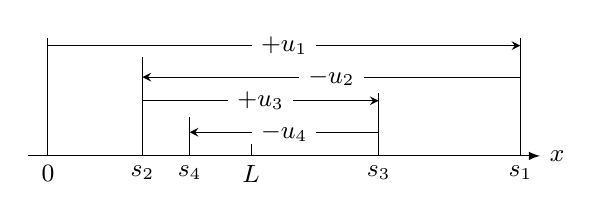
\begin{tikzpicture}[font=\small]
\pgfmathsetmacro{\k}{6}
\pgfmathsetmacro{\b}{0.2*\k}
\pgfmathsetmacro{\c}{0.7*\k}
\pgfmathsetmacro{\d}{0.3*\k}
\draw[-latex](-0.25,0)--(\k+0.25,0)node[right]{$x$};
\draw(0,0)node[below]{$0$}--++(0,1.5);
\draw(\k,0)node[below]{$s_1$}--++(0,1.5);
\draw(\b,0)node[below]{$s_2$}--++(0,1.25);
\draw(\c,0)node[below]{$s_3$}--++(0,0.8);
\draw(\d,0)node[below]{$s_4$}--++(0,0.5);
\draw(0.43*\k,0)node[below]{$L$}--++(0,0.15);
\draw[-stealth](0,1.4)--++(\k,0)node[pos=0.5,fill=white]{$+u_1$};
\draw[-stealth](\k,1)--++({\b-\k},0)node[pos=0.5,fill=white]{$-u_2$};
\draw[-stealth](\b,0.7)--++({\c-\b},0)node[pos=0.5,fill=white]{$+u_3$};
\draw[-stealth](0\c,0.3)--++({\d-\c},0)node[pos=0.5,fill=white]{$-u_4$};
\end{tikzpicture}
\caption{
اس بدلتے  تسلسل کے جزوی مجموعات جو \عددی{N=1} کے لئے مسئلہ \حوالہ{مسئلہ_تسلسل_بدلتا_تسلسل_پرکھ} کے شرائط کو مطمئن کرتا ہو۔
}
\label{شکل_تسلسل_بدلتے_ہندسی_تسلسل_کے_جزوی_مجموعات}
\end{figure}

درج ذیل کی بنا ہم مرتکز بدلتے تسلسل کے مجموعات کی قیمت  کا اندازہ  لگا سکتے ہیں۔
\begin{align*}
\abs{L-s_n}&<u_{n+1}&&n\ge N
\end{align*}

\ابتدا{مسئلہ}\شناخت{مسئلہ_تسلسل_بدلتا_اندازہ}\موٹا{مسئلہ بدلتے تسلسل کا اندازہ}\\
اگر بدلتا تسلسل \عددی{\sum_{n=1}^{\infty}(-1)^{n+1}u_n} مسئلہ \حوالہ{مسئلہ_تسلسل_بدلتا_تسلسل_پرکھ} کے تین شرائط مطمئن کرتا ہو تب \عددی{n\ge N} کے لئے  تسلسل کا مجموعہ \عددی{L} تخمیناً
\begin{align*}
s_n=u_1-u_2+\cdots+(-1)^{n+1}u_n
\end{align*}
ہو گا جس میں مطلق خلل کی قیمت \عددی{u_{n+1}} سے کم ہو گی جو پہلے غیر مستعمل جزو کی عددی قیمت ہے۔ مزید باقی \عددی{L-s_n} کی علامت وہی ہو گی جو پہلی غیر مستعمل جزو کی علامت ہو۔ 
\انتہا{مسئلہ}
%=====================

\ابتدا{مثال}
ہم مسئلہ \حوالہ{مسئلہ_تسلسل_بدلتا_اندازہ} درج ذیل تسلسل پر لاگو کرتے ہیں جس کا مجموعہ ہم جانتے ہیں۔
\begin{align*}
\sum_{n=0}^{\infty}(-1)^n\frac{1}{2^n}=1-\frac{1}{2}+\frac{1}{4}-\frac{1}{8}+\frac{1}{16}-\frac{1}{32}+\frac{1}{64}-\frac{1}{128}\,\protect\rule[-2ex]{0.1ex}{5ex}+\frac{1}{256}-\cdots
\end{align*}
یہ مسئلہ کہتا ہے کہ تسلسل کے آٹھ اجزاء لینے سے ہم  مثبت مقدار رد کرتے ہیں جس کی قیمت \عددی{\tfrac{1}{256}} سے کم ہو گی۔ ابتدائی آٹھ اجزاء کا مجموعہ \عددی{\num{0.6640625}} ہے۔ اس تسلسل کا مجموعہ درج ذیل ہے۔
\begin{align*}
\frac{1}{1-(-1/2)}=\frac{1}{3/2}=\frac{2}{3}
\end{align*}
مجموعہ اور تخمینی قیمت میں فرق \عددی{\tfrac{2}{3}-\num{0.6640625}=\num{0.0026041666}} ہے جو مثبت اور \عددی{\tfrac{1}{256}=\num{0.00390625}} سے کم ہے۔
\انتہا{مثال}
%======================

\جزوحصہء{مطلق ارتکاز}
\ابتدا{تعریف}
تسلسل \عددی{\sum a_n} اس صورت \اصطلاح{مطلق مرتکز}\فرہنگ{مرتکز!مطلق}\حاشیہب{absolutely convergent}\فرہنگ{convergent!absolute} ہو گا جب مطلق قیمتوں کا مطابقتی تسلسل \عددی{\sum \abs{a_n}} مرتکز ہو۔
\انتہا{تعریف}
%====================

ہندسی تسلسل
\begin{align*}
1-\frac{1}{2}+\frac{1}{4}-\frac{1}{8}+\cdots
\end{align*}
مطلق مرتکز ہے چونکہ مطابقتی مطلق قیمتوں کا درج ذیل تسلسل مرتکز ہے۔
\begin{align*}
1+\frac{1}{2}+\frac{1}{4}+\frac{1}{8}+\cdots
\end{align*}
بدلتا ہارمونی تسلسل مطلق مرتکز نہیں ہے چونکہ مطابقتی مطلق قیمتوں کا تسلسل (منفرج) ہارمونی تسلسل ہے۔

\ابتدا{تعریف}
جو تسلسل مرتکز ہو مگر مطلق مرتکز نہ ہو \اصطلاح{مشروط مرتکز}\فرہنگ{مرتکز!مشروط}\حاشیہب{conditional convergent}\فرہنگ{convergent!conditional} کہلاتا ہے۔
\انتہا{تعریف}
%=================

بدلتا ہارمونی تسلسل مشروط مرتکز ہے۔

مطلق ارتکاز دو وجوہات کی بنا اہم ہے۔ پہلی وجہ یہ ہے کہ ہمارے پاس مثبت اجزاء کے تسلسل کی ارتکاز کا اچھے پرکھ ہیں۔ دوسری وجہ یہ کہ کہ مطلق مرتکز تسلسل ہر صورت مرتکز ہو گا۔ یہی اگلے مسئلہ کا موضوع ہے۔

\ابتدا{مسئلہ}\شناخت{مسئلہ_تسلسل_ہر_مطلق_مرتکز_تسلسل_مرتکز}\موٹا{مطلق ارتکاز پرکھ}\\
اگر \عددی{\sum_{n=1}^{\infty}\abs{a_n}} مرتکز ہو تب \عددی{\sum_{n=1}^{\infty}a_n} مرتکز ہو گا۔
\انتہا{مسئلہ}
%=====================
\ابتدا{ثبوت}
ہر \عددی{n} کے لئے
\begin{align*}
-\abs{a_n}\le a_n\le \abs{a_n}\quad \implies \quad 0\le a_n+\abs{a_n}\le 2\abs{a_n}
\end{align*}
ہو گا۔ اگر \عددی{\sum_{n=1}^{\infty}\abs{a_n}} مرتکز ہو تب \عددی{\sum_{n=1}^{\infty}2\abs{a_n}} مرتکز ہو گا اور بلا واسطہ تقابلی پرکھ کے تحت  غیر منفی تسلسل 
\begin{align*}
\sum_{n=1}^{\infty}(a_n+\abs{a_n})
\end{align*}
بھی مرتکز ہو گا۔ ہم مساوات \عددی{a_n=(a_n+\abs{a_n})-\abs{a_n}} کی مدد سے  \عددی{\sum_{n=1}^{\infty}a_n} کو دو مرتکز تسلسل کا فرق 
\begin{align*}
\sum_{n=1}^{\infty}a_n=\sum_{n=1}^{\infty}(a_n+\abs{a_n}-\abs{a_n})=\sum_{n=1}^{\infty}(a_n+\abs{a_n})-\sum_{n=1}^{\infty}\abs{a_n}
\end{align*}
لکھ سکتے ہیں۔یوں \عددی{\sum_{n=1}^{\infty}a_n} مرتکز ہو گا۔
\انتہا{ثبوت}
%==============

ہم مسئلہ \حوالہ{مسئلہ_تسلسل_ہر_مطلق_مرتکز_تسلسل_مرتکز} کو یوں بھی پڑھ سکتے ہیں کہ ہر مطلق مرتکز تسلسل مرتکز ہو گا البتہ ضروری نہیں ہے کہ مرتکز تسلسل مطلق مرتکز ہو۔

\ابتدا{مثال}\شناخت{مثال_تسلسل_درکار_بعد_الف}
تسلسل \عددی{\sum_{n=1}^{\infty}(-1)^{n+1}\tfrac{1}{n^2}=1-\tfrac{1}{4}+\tfrac{1}{9}-\tfrac{1}{16}+\cdots} کا مطابقتی مثبت اجزاء کا تسلسل
\begin{align*}
\sum_{n=1}^{\infty}\frac{1}{n^2}=1+\frac{1}{4}+\frac{1}{9}+\frac{1}{16}+\cdots
\end{align*} 
ہے جو مرتکز ہے۔یوں اصل تسلسل اس لئے مرتکز ہے کہ یہ مطلق مرتکز ہے۔
\انتہا{مثال}
%======================
\ابتدا{مثال}
تسلسل \عددی{\sum_{n=1}^{\infty}\tfrac{\sin n}{n^2}=\tfrac{\sin 1}{1}+\tfrac{\sin 2}{4}+\tfrac{\sin 3}{9}+\cdots} کا مطابقتی مثبت اجزاء کا تسلسل درج ذیل ہے
\begin{align*}
\sum_{n=1}^{\infty}\abs{\frac{\sin n}{n^2}}=\frac{\abs{\sin 1}}{1}+\frac{\abs{\sin 2}}{4}+\frac{\abs{\sin 3}}{9}+\cdots
\end{align*}
جس کا ارتکاز  \عددی{\sum_{n=1}^{\infty}\tfrac{1}{n^2}} کے ساتھ موازنہ کرنے سے دیکھا جا سکتا ہے جہاں ہر \عددی{n} کے لئے \عددی{\abs{\sin n}\le 1} ہو گا۔ چونکہ اصل تسلسل مطلق مرتکز ہے، لہٰذا یہ مرتکز ہو گا۔
\انتہا{مثال}
%======================
\ابتدا{مثال}\موٹا{بدلتا \عددی{p} تسلسل}\\
مثبت مستقل \عددی{p} کی صورت میں ترتیب \عددی{\{\tfrac{1}{n^p}\}}  گھٹتا ترتیب ہے جس کا حد صفر ہے۔ یوں بدلتا \عددی{p} تسلسل
\begin{align*}
\sum_{n=1}^{\infty}\frac{(-1)^{n-1}}{n^p}=1-\frac{1}{2^p}+\frac{1}{3^p}-\frac{1}{4^p}+\cdots,\quad p>0
\end{align*}
مرتکز ہو گا۔

اگر \عددی{p>1} ہو تب یہ مطلق مرتکز تسلسل ہو گا۔ اگر \عددی{p\le 1} ہو تب یہ مشروط مرتکز تسلسل ہو گا۔
\begin{align*}
1-\frac{1}{\sqrt{2}}+\frac{1}{\sqrt{3}}-\frac{1}{\sqrt{4}}+\cdots&&\text{\RL{مشروط مرتکز}}\\
1-\frac{1}{2^{3/2}}+\frac{1}{3^{3/2}}-\frac{1}{4^{3/2}}+\cdots&&\text{\RL{مطلق مرتکز}}
\end{align*}
\انتہا{مثال}
%===================

\جزوحصہء{تسلسل کی ترتیب نو}
\ابتدا{مسئلہ}\شناخت{مسئلہ_تسلسل_ترتیب_نو}\موٹا{مطلق مرتکز تسلسل کا مسئلہ ترتیب نو}\\
اگر \عددی{\sum_{n=1}^{\infty}a_n} مطلق مرتکز ہو اور ترتیب \عددی{\{a_n\}} کے اجزاء کی ترتیب نو  کر کے انہیں \عددی{b_1,b_2,\cdots,b_n,\cdots}  لکھا جائے تب \عددی{\sum b_n} مطلق مرتکز ہو گا اور درج ذیل ہو گا۔
\begin{align*}
\sum_{n=1}^{\infty}a_n=\sum_{n=1}^{\infty}b_n
\end{align*}
\انتہا{مسئلہ}
%==================
(اس مسئلہ کی ثبوت کے خاکہ کے  لئے سوال \حوالہ{سوال_لامتناہی_تسلسل_مسئلہ_ثبوت_درکار} دیکھیں۔)

\ابتدا{مثال}
ہم نے مثال \حوالہ{مثال_تسلسل_درکار_بعد_الف} میں دیکھا کہ تسلسل
\begin{align*}
1-\frac{1}{4}+\frac{1}{9}-\frac{1}{16}+\cdots+(-1)^{n-1}\frac{1}{n^2}+\cdots
\end{align*}
مطلق مرتکز ہے۔ اس کی ترتیب نو کرتے ہوئے ابتدائی جزو مثبت اور اس  کے بعد دو منفی اجزاء منتخب کیے جا سکتے ہیں۔اس کے بعد تین مثبت اور چار منفی اجزاء  منتخب کیے جا سکتے ہیں، وغیرہ وغیرہ۔ یوں ایک ہی علامت کے \عددی{k} اجزاء کے بعد الٹ علامت کے \عددی{k+1} اجزاء ہوں گے۔ ایسے تسلسل کے ابتدائی دس اجزاء درج ذیل ہوں گے۔
\begin{align*}
1-\frac{1}{4}-\frac{1}{16}+\frac{1}{9}+\frac{1}{25}+\frac{1}{49}-\frac{1}{36}-\frac{1}{64}-\frac{1}{100}-\frac{1}{144}+\cdots
\end{align*}
مسئلہ ترتیب نو کے تحت دونوں تسلسل ایک ہی عدد پر مرتکز ہوں گے۔ اس مثال میں (اگر ہم جانتے کہ ایسا ممکن ہے) ہم خوشی سے دوسرے تسلسل کی جگہ پہلا تسلسل استعمال کرنا چاہیں گے۔ اس سے بھی بہتر ہوتا اگر ہم جانتے کہ ان دونوں تسلسل کا مجموعہ درج ذیل کے برابر ہے۔
\begin{align*}
\sum_{n=1}^{\infty}\frac{1}{(2n-1)^2}-\sum_{n=1}^{\infty}\frac{1}{(2n)^2}
\end{align*}
(سوال \حوالہ{سوال_لامتناہی_تسلسل_مطلق_مرتکز_تسلسل_درکار} دیکھیں۔)
\انتہا{مثال}
%======================
\ابتدا{مثال}\شناخت{مثال_تسلسل_بدلتا_ہارمونی_ترتیب_نو}\ترچھا{بدلتے ہارمونی تسلسل کی ترتیب نو}\\
بدلتا ہارمونی تسلسل
\begin{align*}
\frac{1}{1}-\frac{1}{2}+\frac{1}{3}-\frac{1}{4}+\frac{1}{5}-\frac{1}{6}+\frac{1}{7}-\frac{1}{8}+\frac{1}{9}-\frac{1}{10}+\frac{1}{11}-\cdots
\end{align*}
کی ترتیب نو سے منفرج  یا مخصوص قیمت کا تسلسل حاصل کیا جا سکتا ہے۔
\begin{enumerate}[a.]
\item
\عددی{\sum_{n=1}^{\infty}(-1)^{n+1}/n} کی ترتیب نو سے انفراج: \quad
اجزاء \عددی{\sum 1/(2n-1)} کا مجموعہ \عددی{+\infty} کو منفرج جبکہ \عددی{\sum (-1/{2n})} کا مجموعہ \عددی{-\infty} کو منفرج ہے۔ ہم جتنے زیادہ طاق اجزاء کے بعد  مجموعہ کیوں نہ لیں، آخر کار یہ تواتر سے پائے جانے والے اجزاء کا مجموعہ کسی بھی مقررہ قیمت سے بڑا ہو گا۔ اسی طرح ہم  جتنے زیادہ منفی اجزاء کے بعد  مجموعہ کیوں نہ لیں، آخر کار تواتر سے پائے جانے والے جفت اجزاء کا یہ مجموعہ کسی بھی مقررہ منفی قیمت سے زیادہ منفی ہو گا۔ اگر ہم چاہیں، ہم پہلے اتنے طاق اجزاء جمع کر سکتے ہیں کہ ان کا مجموعہ مثلاً \عددی{+3} ہو اور اس کے بعد صرف جفت اجزاء جمع کرتے ہوئے مجموعے کو \عددی{-4} تک پہنچائیں۔ اس کے بعد ہم غیر استعمال شدہ منفی اجزاء شامل کرتے ہوئے کل\عددی{+5} حاصل کر کے اس کے ساتھ اتنے منفی اجزاء شامل کریں کہ \عددی{-6} حاصل ہو، وغیرہ، وغیرہ۔ اس طرح ہم دونوں اطراف جھولا اختیاری زیادہ کر سکتے ہیں۔ 
\item
\عددی{\sum_{n=1}^{\infty}(-1)^{n+1}/n} کی ترتیب سے \عددی{1} پر ارتکاز:\quad
ہم ترتیب نو سے کسی بھی مخصوص قیمت پر بدلتے ہارمونی تسلسل کو مرتکز کر سکتے ہیں۔ فرض کریں ہم \عددی{1} پر مرتکز تسلسل حاصل کرنا چاہتے ہیں۔ ہم پہلے جزو \عددی{\tfrac{1}{1}} سے شروع کر کے \عددی{\tfrac{1}{2}} منفی کرتے ہیں۔ اس کے بعد \عددی{\tfrac{1}{3}} اور \عددی{\tfrac{1}{5}} جمع کرتے ہوئے مجموعہ کو واپس \عددی{1} یا اس سے اوپر تک لاتے ہیں۔ اس کے بعد ہم متواتر منفی اجزاء جمع کرتے ہوئے مجموعہ \عددی{1} سے نیچے لے جاتے ہیں۔ ہم اسی طرح اجزاء جمع اور منفی کیے جاتے ہیں۔ جب مجموعہ \عددی{1} سے تجاوز کرے، ہم منفی اجزاء جمع کرتے ہیں حتٰی کہ مجموعہ \عددی{1} یا اس سے کم ہو جائے۔ اس کے بعد ہم مثبت اجزاء جمع کرتے ہیں جب تک مجموعہ \عددی{1} یا اس سے زیادہ نہ ہو۔ اس طریقہ کار کو غیر معینہ استعمال کیا جا سکتا ہے۔ چونکہ \عددی{n\to \infty} کرنے سے اصل تسلسل کے جفت اور طاق اجزاء کی قیمتیں \عددی{0} تک پہنچتی ہیں لہٰذا  نئی تسلسل کا جزوی مجموعہ  \عددی{1} کے قریب تر ہوتا جائے گا لہٰذا نئے تسلسل کا مجموعہ \عددی{1} پر مرتکز ہو گا۔نیا تسلسل درج ذیل صورت کا ہو گا:
\begin{multline*}
\frac{1}{1}-\frac{1}{2}+\frac{1}{3}+\frac{1}{5}-\frac{1}{4}+\frac{1}{7}+\frac{1}{9}-\frac{1}{6}+\frac{1}{11}+\frac{1}{13}-\frac{1}{8}+\frac{1}{15}+\frac{1}{17}-\frac{1}{10}\\+\frac{1}{19}+\frac{1}{21}-\frac{1}{12}+\frac{1}{23}+\frac{1}{25}-\frac{1}{14}+\frac{1}{27}-\frac{1}{16}+\cdots
\end{multline*}
\end{enumerate}
\انتہا{مثال}
%=====================

آپ نے دیکھا کہ مشروط مرتکز تسلسل کی ترتیب نو کر کے لامتناہی تعداد کے اجزاء جمع کرتے ہوئے  اصل تسلسل سے بہت مختلف مجموعہ حاصل کیا جا سکتا ہے۔ یوں ضروری ہے کہ مشروط مرتکز تسلسل کے اجزاء اسی ترتیب سے جمع کیے جائیں جس ترتیب سے یہ تسلسل میں پائے جاتے ہیں۔  

\حصہء{سوالات}
\موٹا{ارتکاز اور انفراج معلوم کرنا}\\
سوال \حوالہ{سوال_تسلسل_مرتکز_منفرج_بدلتا_الف} تا سوال \حوالہ{سوال_تسلسل_مرتکز_منفرج_بدلتا_ب} میں کونسا بدلتا تسلسل مرتکز اور کونسا منفرج ہے؟ اپنے جواب کی وجہ پیش کریں۔

\ابتدا{سوال}\شناخت{سوال_تسلسل_مرتکز_منفرج_بدلتا_الف}
$\sum\limits_{n=1}^{\infty}(-1)^{n+1}\frac{1}{n^2}$\\
جواب:\quad
مسئلہ \حوالہ{مسئلہ_تسلسل_بدلتا_تسلسل_پرکھ} کے تحت ارتکاز
\انتہا{سوال}
%=====================
\ابتدا{سوال}
$\sum\limits_{n=1}^{\infty}(-1)^{n+1}\frac{1}{n^{3/2}}$
\انتہا{سوال}
%=====================
\ابتدا{سوال}
$\sum\limits_{n=1}^{\infty}(-1)^{n+1}\big(\frac{n}{10}\big)^n$\\
جواب:\quad
انفراج؛ \عددی{a_n\not\to0}
\انتہا{سوال}
%=====================
\ابتدا{سوال}
$\sum\limits_{n=1}^{\infty}(-1)^{n+1}\frac{10^n}{n^{10}}$
\انتہا{سوال}
%=====================
\ابتدا{سوال}
$\sum\limits_{n=2}^{\infty}(-1)^{n+1}\frac{1}{\ln n}$\\
جواب:\quad
مسئلہ \حوالہ{مسئلہ_تسلسل_بدلتا_تسلسل_پرکھ} کے تحت ارتکاز
\انتہا{سوال}
%=====================
\ابتدا{سوال}
$\sum\limits_{n=1}^{\infty}(-1)^{n+1}\frac{\ln n}{n}$
\انتہا{سوال}
%=====================
\ابتدا{سوال}
$\sum\limits_{n=2}^{\infty}(-1)^{n+1}\frac{\ln n}{\ln n^2}$\\
جواب:\quad
انفراج؛ \عددی{a_n\to\tfrac{1}{2}}
\انتہا{سوال}
%=====================
\ابتدا{سوال}
$\sum\limits_{n=1}^{\infty}(-1)^{n}\ln\big(1+\frac{1}{n}\big)$
\انتہا{سوال}
%=====================
\ابتدا{سوال}
$\sum\limits_{n=1}^{\infty}(-1)^{n+1}\big(\frac{\sqrt{n}+1}{n+1}\big)$\\
جواب:\quad
مسئلہ \حوالہ{مسئلہ_تسلسل_بدلتا_تسلسل_پرکھ} کے تحت ارتکاز
\انتہا{سوال}
%=====================
\ابتدا{سوال}\شناخت{سوال_تسلسل_مرتکز_منفرج_بدلتا_ب}
$\sum\limits_{n=1}^{\infty}(-1)^{n+1}\,\frac{3\sqrt{n+1}}{\sqrt{n}+1}$
\انتہا{سوال}
%=====================
\موٹا{مطلق ارتکاز}\\
سوال \حوالہ{سوال_تسلسل_مطلق_مرتکز_مرتکز_منفرج_الف} تا سوال \حوالہ{سوال_تسلسل_مطلق_مرتکز_مرتکز_منفرج_ب} میں کون سے تسلسل مطلق مرتکز، مرتکز اور منفرج ہیں؟ اپنے جواب کی وجہ پیش کریں۔
 
\ابتدا{سوال}\شناخت{سوال_تسلسل_مطلق_مرتکز_مرتکز_منفرج_الف}
$\sum\limits_{n=1}^{\infty}(-1)^{n+1}(0.1)^n$\\
جواب:\quad
مطلق مرتکز۔مطلق قیمتوں کا تسلسل مرتکز ہندسی تسلسل ہے۔
\انتہا{سوال}
%====================
\ابتدا{سوال}
$\sum\limits_{n=1}^{\infty}(-1)^{n+1}\frac{(0.1)^n}{n}$
\انتہا{سوال}
%====================
\ابتدا{سوال}
$\sum\limits_{n=1}^{\infty}(-1)^n\frac{1}{\sqrt{n}}$\\
جواب:\quad
مشروط ارتکاز۔ \عددی{\tfrac{1}{\sqrt{n}}\to 0} لیکن \عددی{\sum_{n=1}^{\infty}\tfrac{1}{\sqrt{n}}} منفرج ہے۔
\انتہا{سوال}
%====================
\ابتدا{سوال}
$\sum\limits_{n=1}^{\infty}\frac{(-1)^n}{1+\sqrt{n}}$
\انتہا{سوال}
%====================
\ابتدا{سوال}
$\sum\limits_{n=1}^{\infty}(-1)^{n+1}\frac{n}{n^3+1}$\\
جواب:\quad
مطلق مرتکز۔ \عددی{\sum_{n=1}^{\infty}\tfrac{1}{n^2}} کے ساتھ موازنہ کریں۔
\انتہا{سوال}
%====================
\ابتدا{سوال}
$\sum\limits_{n=1}^{\infty}(-1)^{n+1}\frac{n!}{2^n}$
\انتہا{سوال}
%====================
\ابتدا{سوال}
$\sum\limits_{n=1}^{\infty}(-1)^n\frac{1}{n+3}$\\
جواب:\quad
مشروط مرتکز۔ \عددی{\tfrac{1}{n+3}\to 0} ہے لیکن \عددی{\sum_{n=1}^{\infty}\tfrac{1}{n+3}} منفرج ہے۔ (\عددی{\sum_{n=1}^{\infty}\tfrac{1}{n}} کے ساتھ موازنہ کریں۔)
\انتہا{سوال}
%====================
\ابتدا{سوال}
$\sum\limits_{n=1}^{\infty}(-1)^n\,\frac{\sin n}{n^2}$
\انتہا{سوال}
%====================
\ابتدا{سوال}
$\sum\limits_{n=1}^{\infty}(-1)^{n+1}\,\frac{3+n}{5+n}$\\
جواب:\quad
انفراج: \عددی{\tfrac{3+n}{5+n}\to 1}
\انتہا{سوال}
%====================
\ابتدا{سوال}
$\sum\limits_{n=2}^{\infty}(-1)^n\frac{1}{\ln (n^3)}$
\انتہا{سوال}
%====================
\ابتدا{سوال}
$\sum\limits_{n=1}^{\infty}(-1)^{n+1}\,\frac{1+n}{n^2}$\\
جواب:\quad
مشروط مرتکز۔ \عددی{(\tfrac{1}{n^2}-\tfrac{1}{n})\to 0} لیکن \عددی{\tfrac{1+n}{n^2}>\tfrac{1}{n}} ہے۔
\انتہا{سوال}
%====================
\ابتدا{سوال}
$\sum\limits_{n=1}^{\infty}\frac{(-2)^{n+1}}{n+5^n}$
\انتہا{سوال}
%====================
\ابتدا{سوال}
$\sum\limits_{n=1}^{\infty}(-1)^{n} n^2(2/3)^n$\\
جواب:\quad
مطلق ارتکاز؛ جذری پرکھ
\انتہا{سوال}
%====================
\ابتدا{سوال}
$\sum\limits_{n=1}^{\infty}(-1)^{n+1}(\sqrt[n]{10})$
\انتہا{سوال}
%====================
\ابتدا{سوال}
$\sum\limits_{n=1}^{\infty}(-1)^n\frac{\tan^{-1}n}{n^2+1}$\\
جواب:\quad
مطلق ارتکاز۔ تکملی پرکھ
\انتہا{سوال}
%====================
\ابتدا{سوال}
$\sum\limits_{n=2}^{\infty}(-1)^{n+1}\,\frac{1}{n\ln n}$
\انتہا{سوال}
%====================
\ابتدا{سوال}
$\sum\limits_{n=1}^{\infty}(-1)^n\frac{n}{n+1}$\\
جواب:\quad
منفرج؛ \عددی{a_n\not\to 0}
\انتہا{سوال}
%====================
\ابتدا{سوال}
$\sum\limits_{n=1}^{\infty}(-1)^n\frac{\ln n}{n-\ln n}$
\انتہا{سوال}
%====================
\ابتدا{سوال}
$\sum\limits_{n=1}^{\infty}\frac{(-100)^n}{n!}$\\
جواب:\quad
مطلق مرتکز۔ تناسبی پرکھ
\انتہا{سوال}
%====================
\ابتدا{سوال}
$\sum\limits_{n=1}^{\infty}(-5)^{-n}$
\انتہا{سوال}
%====================
\ابتدا{سوال}
$\sum\limits_{n=1}^{\infty}\frac{(-1)^{n-1}}{n^2+2n+1}$\\
جواب:\quad
مطلق مرتکز: \عددی{\tfrac{1}{n^2+2n+1}<\tfrac{1}{n^2}}
\انتہا{سوال}
%====================
\ابتدا{سوال}
$\sum\limits_{n=2}^{\infty}(-1)^n\big(\frac{\ln n}{\ln n^2}\big)^n$
\انتہا{سوال}
%====================
\ابتدا{سوال}
$\sum\limits_{n=1}^{\infty}\frac{\cos n\pi}{n\sqrt{n}}$\\
جواب:\quad
مطلق ارتکاز (مرتکز \عددی{p} تسلسل):  
$\abs{\tfrac{\cos n\pi}{n\sqrt{n}}}=\abs{\tfrac{(-1)^{n+1}}{n^{3/2}}}=\tfrac{1}{n^{3/2}}$
\انتہا{سوال}
%====================
\ابتدا{سوال}
$\sum\limits_{n=1}^{\infty}\frac{\cos n\pi}{n}$
\انتہا{سوال}
%====================
\ابتدا{سوال}
$\sum\limits_{n=1}^{\infty}\frac{(-1)^n(n+1)^n}{(2n)^n}$\\
جواب:\quad
مطلق مرتکز۔ جذری پرکھ
\انتہا{سوال}
%====================
\ابتدا{سوال}
$\sum\limits_{n=1}^{\infty}\frac{(-1)^{n+1}(n!)^2}{(2n)!}$
\انتہا{سوال}
%====================
\ابتدا{سوال}
$\sum\limits_{n=1}^{\infty}(-1)^n\frac{(2n)!}{2^nn!n}$\\
جواب:\quad
منفرج: \عددی{a_n\to\infty}
\انتہا{سوال}
%====================
\ابتدا{سوال}
$\sum\limits_{n=1}^{\infty}(-1)^n\frac{(n!)^23^n}{(2n+1)!}$
\انتہا{سوال}
%====================
\ابتدا{سوال}
$\sum\limits_{n=1}^{\infty}(-1)^n(\sqrt{n+1}-\sqrt{n})$\\
جواب:\quad
مشروط مرتکز: \عددی{\sqrt{n+1}-\sqrt{n}=\tfrac{1}{\sqrt{n}+\sqrt{n+1}}\to0} لیکن مطلق قیمتوں کا تسلسل منفرج ہوتا ہے۔ (\عددی{\sum\tfrac{1}{n}} کے ساتھ موازنہ کریں۔) 
\انتہا{سوال}
%====================
\ابتدا{سوال}
$\sum\limits_{n=1}^{\infty}(-1)^n(\sqrt{n^2+n}-n)$
\انتہا{سوال}
%====================
\ابتدا{سوال}
$\sum\limits_{n=1}^{\infty}(-1)^n(\sqrt{n+\sqrt{n}}-\sqrt{n})$\\
جواب:\quad
منفرج: \عددی{a_n\to \tfrac{1}{2}\ne 0}
\انتہا{سوال}
%====================
\ابتدا{سوال}
$\sum\limits_{n=1}^{\infty}\frac{(-1)^n}{\sqrt{n}+\sqrt{n+1}}$
\انتہا{سوال}
%====================
\ابتدا{سوال}
$\sum\limits_{n=1}^{\infty}(-1)^n\sech n$\\
جواب:\quad
مطلق مرتکز: 
$\sech n=\tfrac{2}{e^n+e^{-n}}=\tfrac{2e^n}{e^{2n}+1}<\tfrac{2e^n}{e^{2n}}=\tfrac{2}{e^n}$ 
اور \عددی{\tfrac{2}{e^n}} مرتکز ہندسی تسلسل کا ایک جزو ہے۔
\انتہا{سوال}
%====================
\ابتدا{سوال}\شناخت{سوال_تسلسل_مطلق_مرتکز_مرتکز_منفرج_ب}
$\sum\limits_{n=1}^{\infty}(-1)^n\csch n$
\انتہا{سوال}
%====================

\موٹا{خلل کا اندازہ}\\
سوال \حوالہ{سوال_تسلسل_خلل_چار_اجزاء_الف} تا سوال \حوالہ{سوال_تسلسل_خلل_چار_اجزاء_ب} میں ابتدائی چار اجزاء سے تخمینی مجموعہ حاصل کرنے سے پیدا خلل کا اندازہ لگائیں۔

\ابتدا{سوال}\شناخت{سوال_تسلسل_خلل_چار_اجزاء_الف}
$\sum\limits_{n=1}^{\infty}(-1)^{n+1}\,\frac{1}{n}$\quad
اس تسلسل کا مجموعہ \عددی{\ln 2} ہے۔\\
جواب:\quad
$\abs{\text{خلل}}<0.2$
\انتہا{سوال}
%=========================
\ابتدا{سوال}
$\sum\limits_{n=1}^{\infty}(-1)^{n+1}\frac{1}{10^n}$
\انتہا{سوال}
%=======================
\ابتدا{سوال}
$\sum\limits_{n=1}^{\infty}(-1)^{n+1}\frac{(0.01)^n}{n}$\quad
جیسا آپ حصہ \حوالہ{حصہ_تسلسل_ٹیلر_اور_اندازہ_خلل} میں دیکھیں گے اس تسلسل کا مجموعہ \عددی{\ln(1.01)} ہے۔\\
جواب:\quad
$\abs{\text{خلل}}<2\times 10^{-11}$
\انتہا{سوال}
%=======================
\ابتدا{سوال}\شناخت{سوال_تسلسل_خلل_چار_اجزاء_ب}
$\frac{1}{1+t}=\sum\limits_{n=1}^{\infty}(-1)^nt^n,\quad 0<t<1$
\انتہا{سوال}
%=======================
\ترچھا{کیلکولیٹر کا استعمال}\\
سوال \حوالہ{سوال_تسلسل_مطلق_خلل_الف} اور سوال \حوالہ{سوال_تسلسل_مطلق_خلل_ب} میں مجموعہ کی تخمینی قیمت تلاش کریں جس میں خلل کی مقدار \عددی{5\times 10^{-6}} سے کم ہو۔

\ابتدا{سوال}\شناخت{سوال_تسلسل_مطلق_خلل_الف}
$\sum\limits_{n=0}^{\infty}(-1)^n\frac{1}{(2n)!}$\quad
جیسا آپ حصہ \حوالہ{حصہ_تسلسل_ٹیلر_اور_اندازہ_خلل} میں دیکھیں گے  اس کا مجموعہ \عددی{\cos1} ہے جہاں \عددی{1} ریڈیئن میں ہے۔\\
جواب:\quad
\عددی{0.54030}
\انتہا{سوال}
%=====================
\ابتدا{سوال}\شناخت{سوال_تسلسل_مطلق_خلل_ب}
$\sum\limits_{n=0}^{\infty}(-1)^n\frac{1}{n!}$\quad
جیسا آپ حصہ \حوالہ{حصہ_تسلسل_ٹیلر_اور_اندازہ_خلل} میں دیکھیں گے  اس کا مجموعہ \عددی{e^{-1}} ہے۔ 
\انتہا{سوال}
%=====================
\موٹا{نظریہ اور مثالیں}\\
\ابتدا{سوال}
(الف) تسلسل \عددی{\tfrac{1}{3}-\tfrac{1}{2}+\tfrac{1}{9}-\tfrac{1}{4}+\tfrac{1}{27}-\tfrac{1}{8}+\cdots+\tfrac{1}{3^n}-\tfrac{1}{2^n}+\cdots} مسئلہ \حوالہ{مسئلہ_تسلسل_بدلتا_تسلسل_پرکھ} کے کس ایک شرط کو مطمئن نہیں کرتا ہے؟ (ب) اس تسلسل کا مجموعہ تلاش کریں۔\\
جواب:\quad
(الف) \عددی{a_n\ge a_{n+1}} (ب) \عددی{-\tfrac{1}{2}}
\انتہا{سوال}
%==================
\ابتدا{سوال}\ترچھا{کیلکولیٹر}\\
مسئلہ \حوالہ{مسئلہ_تسلسل_بدلتا_تسلسل_پرکھ} کے شرائط کو مطمئن کرنے والے بدلتے تسلسل کا حد \عددی{L} کسی بھی دو یک بعد دیگرے جزوی مجموعوں کے بیچ پایا جاتا ہے۔ یوں ہم \عددی{L} کی اندازاً قیمت کے لئے اوسط \عددی{\tfrac{s_n+s_{n+1}}{2}=s_n+\tfrac{1}{2}(-1)^{n+2}a_{n+1}} استعمال کر سکتے ہیں۔ بدلتے ہارمونی تسلسل کا تخمینی مجموعہ \عددی{s_{20}+\tfrac{1}{2}\cdot\tfrac{1}{21}} کا حساب لگائیں۔ ٹھیک ٹھیک مجموعہ \عددی{\ln 2=0.6931\cdots} ہے۔
\انتہا{سوال}
%==================
\ابتدا{سوال}\ترچھا{بدلتا تسلسل جو مسئلہ \حوالہ{مسئلہ_تسلسل_بدلتا_تسلسل_پرکھ} کے شرائط مطمئن کرتا ہو کے جزوی مجموعہ کے باقی علامت}\\
مسئلہ \حوالہ{مسئلہ_تسلسل_بدلتا_اندازہ} کہتا ہے کہ جب مسئلہ \حوالہ{مسئلہ_تسلسل_بدلتا_تسلسل_پرکھ} کے شرائط مطمئن کرنے والے تسلسل  کے مجموعہ کو تخمیناً اس کے جزوی مجموعہ سے ظاہر کیا جائے تب تسلسل کے باقی اجزاء کے مجموعہ کی علامت پہلے غیر مستعمل جزو کی علامت ہو گی۔ اس فقرے کو ثابت کریں۔ (اشارہ: باقی اجزاء کو دو دو کی گروہوں میں جمع کریں۔)
\انتہا{سوال}
%===============
\ابتدا{سوال}
دکھائیں کہ تسلسل \عددی{1-\tfrac{1}{2}+\tfrac{1}{2}-\tfrac{1}{3}+\tfrac{1}{3}-\tfrac{1}{4}+\tfrac{1}{4}-\tfrac{1}{5}+\tfrac{1}{5}-\tfrac{1}{6}+\cdots} کے ابتدائی \عددی{2n} اجزاء کا مجموعہ درج ذیل تسلسل کے ابتدائی \عددی{n} اجزاء کے مجموعہ کے برابر ہو گا۔
\begin{align*}
\frac{1}{1\cdot 2}+\frac{1}{2\cdot 3}+\frac{1}{3\cdot 4}+\frac{1}{4\cdot 5}+\frac{1}{5\cdot 6}+\cdots
\end{align*}
کیا یہ تسلسل مرتکز ہیں؟ ابتدائی \عددی{2n+1} اجزاء کا مجموعہ کتنا ہے؟ اگر تسلسل مرتکز ہوں تب ان کا مجموعہ کتنا ہے؟
\انتہا{سوال}
%====================
\ابتدا{سوال}
دکھائیں کہ اگر \عددی{\sum_{n=1}^{\infty}a_n} منفرج تب \عددی{\sum_{n=1}^{\infty}\abs{a_n}} بھی منفرج ہو گا۔
\انتہا{سوال}
%====================
\ابتدا{سوال}
دکھائیں اگر \عددی{\sum_{n=1}^{\infty}a_n} مطلق مرتکز ہو تب \عددی{\abs{\sum_{n=1}^{\infty}a_n}\le \sum_{n=1}^{\infty}\abs{a_n}} ہو گا۔
\انتہا{سوال}
%==================
\ابتدا{سوال}
دکھائیں اگر \عددی{\sum_{n=1}^{\infty}a_n} اور \عددی{\sum_{n=1}^{\infty}b_n} دونوں مطلق مرتکز ہوں درج ذیل بھی مطلق مرتکز ہوں گے۔
\begin{multicols}{3}
\begin{enumerate}[a.]
\item
$\sum_{n=1}^{\infty}(a_n+b_n)$
\item
$\sum_{n=1}^{\infty}(a_n-b_n)$
\item
$\sum_{n=1}^{\infty}ka_n$\quad
(\عددی{k} عدد ہے)
\end{enumerate}
\end{multicols}
\انتہا{سوال}
%==================
\ابتدا{سوال}
مثال دے کر دکھائیں کہ مرتکز \عددی{\sum_{n=1}^{\infty}a_n} اور مرتکز \عددی{\sum_{n=1}^{\infty}b_n} کے باوجود 
\عددی{\sum_{n=1}^{\infty}a_n\cdot b_n} منفرج ہو سکتا ہے۔
\انتہا{سوال}
%===================
\ابتدا{سوال}
آپ چاہتے ہیں کہ مثال \حوالہ{مثال_تسلسل_بدلتا_ہارمونی_ترتیب_نو} میں ترتیب نو سے ایسا تسلسل حاصل کریں جس کا مجموعہ \عددی{-\tfrac{1}{2}} ہو۔نئے تسلسل کو \عددی{-\tfrac{1}{2}} سے شروع کریں۔جب بھی مجموعہ \عددی{-\tfrac{1}{2}} کے برابر یا اس سے کم ہو، یک بعد دیگرے مثبت اجزاء  شامل کریں حتٰی کہ مجموعہ \عددی{-\tfrac{1}{2}} سے بڑا ہو۔ اس کے بعد منفی اجزاء شامل کریں حتٰی کہ مجموعہ \عددی{-\tfrac{1}{2}} کے برابر یا اس سے کم ہو۔ اسی طرح چلتے جائیں حتٰی کہ جزوی مجموعات \عددی{-\tfrac{1}{2}} سے تین مرتبہ تجاوز کر جائیں اور یہیں رک جائیں یا اس سے ایک قدم پہلے رک جائیں۔ اگر ابتدائی \عددی{n} نئے اجزاء کا مجموعہ \عددی{s_n} ہو تب \عددی{(n,s_n)} ترسیم کر کے جزوی مجموعات کا رویہ واضح کریں۔
\انتہا{سوال}
%====================
\ابتدا{سوال}\شناخت{سوال_لامتناہی_تسلسل_مسئلہ_ثبوت_درکار}\ترچھا{مسئلہ \حوالہ{مسئلہ_تسلسل_ترتیب_نو} کے ثبوت کا خاکہ}\\
\begin{enumerate}[a.]
\item
فرض کریں \عددی{\epsilon} ایک مثبت حقیقی عدد ہو۔ مزید فرض کریں \عددی{L=\sum_{n=1}^{\infty}a_n} اور \عددی{s_k=\sum_{n=1}^{k}a_n} ہیں۔  دکھائیں کہ کسی اشاریہ \عددی{N_1} کے لئے اور کسی اشاریہ \عددی{N_2\ge N_1} کے لئے 
\عددی{\sum_{n=N_1}^{\infty}\abs{a_n}\le \tfrac{\epsilon}{2}} اور \عددی{\abs{s_{N_2}-L}<\tfrac{\epsilon}{2}} ہوں گے۔ چونکہ تمام اجزاء \عددی{a_1,a_2,\cdots,a_{N_2}}  ترتیب \عددی{\{b_n\}} میں کہیں نا کہیں پائے جاتے ہیں لہٰذا ایک ایسا اشاریہ \عددی{N_3\ge N_2} پایا جائے گا کہ اگر \عددی{n\ge N_3} ہو تب \عددی{(\sum_{k=1}^{n}b_k)-s_{N_2}} زیادہ سے زیادہ اجزاء \عددی{a_m} کا مجموعہ ہو گا جہاں \عددی{m\ge N_1} ہے۔یوں اگر  \عددی{n\ge N_3} تب  درج ذیل ہو گا۔
\begin{align*}
\abs{\sum_{k=1}^{n}b_k-L}\le \abs{\sum_{k=1}^{n}b_k-s_{N_2}}+\abs{s_{N_2}-L}\\
\le \sum_{k=N_1}^{\infty}\abs{a_k}+\abs{s_{N_2}-L}<\epsilon
\end{align*}
\item
جزو-الف کی بحث کے تحت اگر \عددی{\sum_{n=1}^{\infty}a_n} مطلق مرتکز ہو تب \عددی{\sum_{n=1}^{\infty}b_n} مرتکز اور
 \عددی{\sum_{n=1}^{\infty}b_n=\sum_{n=1}^{\infty}a_n} ہو گا۔ اب دکھائیں کہ چونکہ \عددی{\sum_{n=1}^{\infty}\abs{a_n}} مرتکز ہے لہٰذا \عددی{\sum_{n=1}^{\infty}\abs{a_n}} پر \عددی{\sum_{n=1}^{\infty}\abs{b_n}} مرتکز ہو گا۔
\end{enumerate}
\انتہا{سوال}
%===================
\ابتدا{سوال}\شناخت{سوال_لامتناہی_تسلسل_مطلق_مرتکز_تسلسل_درکار}
\begin{enumerate}[a.]
\item
دکھائیں اگر \عددی{\sum_{n=1}^{\infty}\abs{a_n}} مرتکز ہو اور \عددی{b_n=\begin{cases} a_n& a_n\ge 0\\ 0& a_n<0  \end{cases}} ہو تب \عددی{\sum_{n=1}^{\infty}b_n} مرتکز ہو گا۔
\item
جزو-ا کا نتیجہ استعمال کرتے ہوئے اسی طرح دکھائیں کہ اگر \عددی{\sum_{n=1}^{\infty}\abs{a_n}} مرتکز ہو اور
 \عددی{c_n=\begin{cases} 0&a_n\ge 0\\ a_n&a_n<0  \end{cases}} ہو تب  \عددی{\sum_{n=1}^{\infty}c_n} مرتکز ہو گا۔

دوسرے لفظوں میں مطلق مرتکز تسلسل کی صورت میں اس کے مثبت اجزاء مرتکز تسلسل بناتے ہیں اور اس کے منفی اجزاء مرتکز تسلسل بناتے ہیں۔مزید \عددی{b_n=\tfrac{a_n+\abs{a_n}}{2}} اور \عددی{c_n=\tfrac{a_n-\abs{a_n}}{2}} کی بنا
 \عددی{\sum_{n=1}^{\infty}a_n=\sum_{n=1}^{\infty}b_n+\sum_{n=1}^{\infty}c_n} ہو گا۔
\end{enumerate}
\انتہا{سوال}
%===================
\ابتدا{سوال}
یہاں کیا غلط ہے:\\
بدلتے ہارمونی تسلسل
\begin{align*}
S=1-\frac{1}{2}+\frac{1}{3}-\frac{1}{4}+\frac{1}{5}-\frac{1}{6}+\frac{1}{7}-\frac{1}{8}+\frac{1}{9}-\frac{1}{10}+\frac{1}{11}-\frac{1}{12}+\cdots
\end{align*}
کے دونوں اطراف کو \عددی{2} سے ضرب دے کر
\begin{align*}
2S=2-1+\frac{2}{3}-\frac{1}{2}+\frac{2}{5}-\frac{1}{3}+\frac{2}{7}-\frac{1}{4}+\frac{2}{9}-\frac{1}{5}+\frac{2}{11}-\frac{1}{6}+\cdots
\end{align*}
حاصل کریں۔ ایک جیسے نسب نما کی اجزاء جمع کریں، مثلاً \عددی{\tfrac{2}{3}-\tfrac{1}{3}} اور \عددی{\tfrac{2}{5}-\tfrac{1}{5}}۔یوں
\begin{align*}
2S=1-\frac{1}{2}+\frac{1}{3}-\frac{1}{4}+\frac{1}{5}-\frac{1}{6}+\cdots
\end{align*}
حاصل ہو گا جہاں بائیں ہاتھ کا تسلسل وہی ہے جہاں سے ہم نے شروع کیا تھا۔یوں \عددی{2S=S} ہو گا جس کے دونوں اطراف کو \عددی{S} سے تقسیم کر کے \عددی{2=1} ملتا ہے۔
\انتہا{سوال}
%==================
\ابتدا{سوال}\شناخت{سوال_لامتناہی_ترسیمی_موازنہ_درکار}
\عددی{N>1} کی صورت میں مسئلہ \حوالہ{مسئلہ_تسلسل_بدلتا_تسلسل_پرکھ} میں تسلسل کا ارتکاز شکل \حوالہ{شکل_تسلسل_بدلتے_ہندسی_تسلسل_کے_جزوی_مجموعات} کی طرح ترسیم بنا کر دکھائیں۔
\انتہا{سوال}
%======================

\حصہ{طاقتی تسلسل}
اب چونکہ ہم لامتناہی تسلسل کا ارتکاز پرکھ سکتے ہیں لہٰذا ہم اب لامتناہی کثیر رکنی کا مطالعہ کر سکتے ہیں جن کا ذکر حصہ \حوالہ{حصہ_تسلسل_لامتناہی} کی شروع میں کیا گیا۔ تعریف کی رو سے ان کثیر رکنیوں کو کسی متغیر، مثلاً \عددی{x}،  کے طاقتوں کا لامتناہی تسلسل لکھا جاتا ہے لہٰذا ہم ان کثیر رکنیوں کو طاقتی تسلسل کہتے ہیں۔ کثیر رکنیوں کی طرح، طاقتی تسلسلوں کو جمع، منفی، ضرب، تفرق اور تکمل کر کے نئے طاقتی تسلسل حاصل کئے جا سکتے ہیں۔

\جزوحصہء{طاقتی تسلسل اور ارتکاز}
ہم با ضابطہ تعریف سے ابتدا کرتے ہیں۔

\ابتدا{تعریف}
نقطہ \عددی{x=0} کے لحاظ سے \اصطلاح{طاقتی تسلسل}\فرہنگ{تسلسل!طاقتی}\فرہنگ{طاقتی تسلسل}\حاشیہب{power series}\فرہنگ{series!power} سے مراد درج ذیل صورت کا تسلسل ہے۔
\begin{align}\label{مساوات_تسلسل_تعریف_طاقتی_الف}
\sum_{n=0}^{\infty}c_nx^n=c_0+c_1x+c_2x^2+\cdots+c_nx^n+\cdots
\end{align}
نقطہ \عددی{x=a} کے لحاظ سے طاقتی تسلسل سے مراد درج ذیل صورت کا تسلسل ہے
\begin{align}\label{مساوات_تسلسل_تعریف_طاقتی_ب}
\sum_{n=0}^{\infty}c_n(x-a)^n=c_0+c_1(x-a)+c_2(x-a)^2+\cdots+c_n(x-a)^n+\cdots
\end{align}
جس میں \اصطلاح{مرکز}\فرہنگ{طاقتی تسلسل!مرکز}\حاشیہب{center}\فرہنگ{series!center} \عددی{a} اور \اصطلاح{عددی سر}\فرہنگ{عددی سر}\حاشیہب{coefficients}\فرہنگ{series!coefficients} \عددی{c_0}، \عددی{c_1}، \عددی{c_2}، \نقطے،\عددی{c_n}،\نقطے مستقل ہیں۔
\انتہا{تعریف}
%===================

مساوات \حوالہ{مساوات_تسلسل_تعریف_طاقتی_ب} میں \عددی{a=0} پر کرنے سے طاقتی تسلسل کی خصوصی روپ مساوات \حوالہ{مساوات_تسلسل_تعریف_طاقتی_الف} حاصل ہوتی ہے۔

\ابتدا{مثال}\شناخت{مثال_تسلسل_تفاعل_اور_تخمینی_کثیر_رکنیاں_الف}
مساوات \حوالہ{مساوات_تسلسل_تعریف_طاقتی_الف} میں تمام عددی سر \عددی{1} لینے سے درج ذیل ہندسی طاقتی تسلسل حاصل ہوتا ہے۔
\begin{align*}
\sum_{n=0}^{\infty}x^n=1+x+x^2+\cdots+x^n+\cdots
\end{align*}
اس ہندسی تسلسل کا پہلا جزو \عددی{1} اور نسبت \عددی{x} ہے۔ یہ \عددی{\abs{x}<1} کے لئے \عددی{\tfrac{1}{1-x}} پر مرتکز ہے۔ اس حقیقت کا اظہار درج ذیل لکھ کر کیا جاتا ہے۔
\begin{align}\label{مساوات_تسلسل_تعریف_طاقتی_پ}
\frac{1}{1-x}=1+x+x^2+\cdots+x^n+\cdots,\quad\quad -1<x<1
\end{align}
\انتہا{مثال}
%================

اب تک مساوات \حوالہ{مساوات_تسلسل_تعریف_طاقتی_ب} کو ہم دائیں ہاتھ تسلسل کے مجموعہ کا کلیہ استعمال کرتے آ رہے ہیں۔ ہم اب اپنی توجہ کا مرکز تبدیل کرتے ہیں۔ ہم دائیں ہاتھ تسلسل کے جزوی مجموعات کو کثیر رکنیاں \عددی{P_n(x)} تصور کرتے ہیں جو بائیں ہاتھ تفاعل کی تخمین دیتے ہیں۔ صفر کے قریب \عددی{x} کی قیمتوں کے لئے تفاعل کی قیمت حاصل کرنے کی خاطر ہم تسلسل کے ابتدائی چند اجزاء کا مجموعہ لے کر تفاعل کی اچھی تخمینی قیمت تلاش کر سکتے ہیں۔ ہاں \عددی{x=-1} یا \عددی{x=1} کے قریب ہمیں تفاعل کی اچھی تخمین حاصل کرنے کی خاطر تسلسل کے زیادہ اجزاء کا مجموعہ لینا ہو گا شکل \حوالہ{شکل_تسلسل_زیادہ_اجزاء_لینے_ہوں_گے} میں تفاعل \عددی{f(x)=\tfrac{1}{1-x}} اور اس کی تخمینی کثیر رکنیاں \عددی{y_n=P_n(x)} دکھائی گئی ہیں۔
\begin{figure}
\centering
\begin{minipage}{0.45\textwidth}
\centering
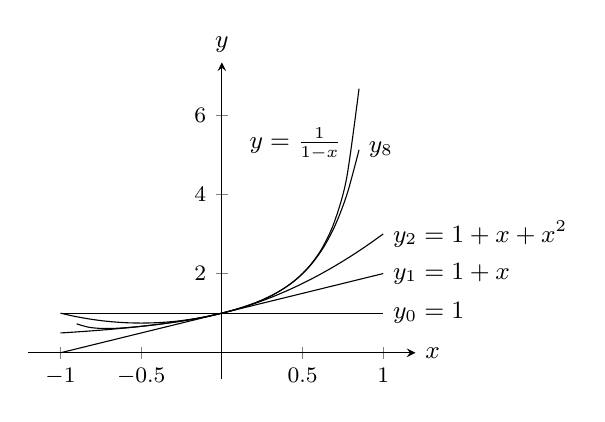
\begin{tikzpicture}[font=\small,declare function={fa(\x)=1;fb(\x)=1+\x;fc(\x)=1+\x+\x^2;fd(\x)=1+\x+\x^2+\x^3+\x^4+\x^5+\x^6+\x^7+\x^8;}]
\begin{axis}[clip=false,small,axis lines=middle, xlabel={$x$},ylabel={$y$},xlabel style={at={(current axis.right of origin)},anchor=west},ylabel style={at={(current axis.above origin)},anchor=south},enlargelimits=true]
\addplot[domain=-1:1]{fa(x)}node[right]{$y_0=1$};
\addplot[domain=-1:1]{fb(x)}node[right]{$y_1=1+x$};
\addplot[smooth,domain=-1:1]{fc(x)}node[right]{$y_2=1+x+x^2$};
\addplot[smooth,domain=-0.9:0.85]{fd(x)}node[right]{$y_8$};
\addplot[smooth,domain=-1:0.85]{1/(1-x)}node[pos=0.8,left]{$y=\frac{1}{1-x}$};
\end{axis}
\end{tikzpicture}
\caption{تفاعل \عددی{f(x)=\tfrac{1}{1-x}} اور اس کی چار تخمینی کثیر رکنیاں (مثال \حوالہ{مثال_تسلسل_تفاعل_اور_تخمینی_کثیر_رکنیاں_الف})۔}
\label{شکل_تسلسل_زیادہ_اجزاء_لینے_ہوں_گے}
\end{minipage}\hfill
\begin{minipage}{0.45\textwidth}
\centering
\begin{tikzpicture}[font=\small,declare function={f(\x)=1;fa(\x)=2-1/2*\x;fb(\x)=3-3/2*\x+1/4*\x^2;}]
\begin{axis}[clip=false,small,axis lines=middle, xlabel={$x$},ylabel={$y$},xlabel style={at={(current axis.right of origin)},anchor=west},ylabel style={at={(current axis.above origin)},anchor=south},enlargelimits=true,xmax=5]
\addplot[domain=0.25:3]{f(x)}node[pos=0.2,above]{$y_0=1$};
\addplot[domain=0.25:3.5]{fa(x)}node[pin=10:{$y_1=2-\frac{x}{2}$}]{};
\addplot[domain=0.75:3.5]{fb(x)}node[pin=80:{$y_1=3-\frac{3x}{2}+\frac{x^2}{4}$}]{};
\addplot[domain=0.75:3.5]{2/x}node[pin=30:{$y=\frac{2}{x}$}]{};
\draw(2,1)node[circ]{}node[below left]{$(2,1)$};
\end{axis}
\end{tikzpicture}
\caption{تفاعل \عددی{f(x)=\tfrac{2}{x}} اور اس کی ابتدائی تین تخمینی کثیر رکنیاں (مثال \حوالہ{مثال_تسلسل_تفاعل_اور_تخمینی_کثیر_رکنیاں_ب})۔}
\label{شکل_تسلسل_تفاعل_کی_تخمینی_کثیر_رکنیاں}
\end{minipage}
\end{figure}

\ابتدا{مثال}\شناخت{مثال_تسلسل_تفاعل_اور_تخمینی_کثیر_رکنیاں_ب}
درج ذیل طاقتی تسلسل مساوات \حوالہ{مساوات_تسلسل_تعریف_طاقتی_ب} کی طرح ہے جہاں \عددی{a=2}، \عددی{c_0=1}، \عددی{c_1=-\tfrac{1}{2}}، \عددی{c_2=\tfrac{1}{4}}، \نقطے،\عددی{c_n=(-1/2)^n} ہیں۔
\begin{align}\label{مساوات_تسلسل_تعریف_طاقتی_ت}
1-\frac{1}{2}(x-2)+\frac{1}{4}(x-2)^2+\cdots+\big(-\frac{1}{2}\big)^n(x-2)^n+\cdots
\end{align}
یہ ایک ہندسی تسلسل ہے جس کا ابتدائی جزو \عددی{1} اور نسبت \عددی{r=-\tfrac{x-2}{2}} ہے۔ یہ تسلسل \عددی{\abs{\tfrac{x-2}{2}}<1} یعنی \عددی{0<x<4} کے لئے مرکوز ہے۔اس کا مجموعہ
\begin{align*}
\frac{1}{1-r}=\frac{1}{1+\tfrac{x-2}{2}}=\frac{2}{x}
\end{align*}
ہے لہٰذا
\begin{align*}
\frac{2}{x}=1-\frac{1}{2}(x-2)+\frac{1}{4}(x-2)^2+\cdots+\big(-\frac{1}{2}\big)^n(x-2)^n+\cdots,\quad 0<x<4
\end{align*}
ہو گا۔ مساوات \حوالہ{مساوات_تسلسل_تعریف_طاقتی_ت} کا تسلسل \عددی{2} کے قریب \عددی{x} کی قیمتوں کے لئے  \عددی{f(x)=\tfrac{2}{x}} کی کارآمد تخمینی کثیر رکنیاں پیدا کرتا ہے (شکل \حوالہ{شکل_تسلسل_تفاعل_کی_تخمینی_کثیر_رکنیاں}):
\begin{align*}
P_0(x)&=1\\
P_1(x)&=1-\frac{1}{2}(x-2)=2-\frac{x}{2}\\
P_2(x)&=1-\frac{1}{2}(x-2)+\frac{1}{4}(x-2)^2=3-\frac{3x}{2}+\frac{x^2}{4}
\end{align*}
\انتہا{مثال}
%======================
\ابتدا{مثال}\شناخت{مثال_تسلسل_مرتکز_منفرج_تسلسل}
درج ذیل طاقتی تسلسل \عددی{x} کی کن قیمتوں کے لئے ارتکاز پذیر ہے؟
\begin{align*}
\sum_{n=1}^{\infty}(-1)^{n-1}\,\frac{x^n}{n}&=x-\frac{x^2}{2}+\frac{x^3}{3}-\cdots&&\text{\RL{(ا)}}\\
\sum_{n=1}^{\infty}(-1)^{n-1}\,\frac{x^{2n-1}}{2n-1}&=x-\frac{x^3}{3}+\frac{x^5}{5}-\cdots&&\text{\RL{(ب)}}\\
\sum_{n=0}^{\infty}\frac{x^n}{n!}&=1+x+\frac{x^2}{2!}+\frac{x^3}{3!}+\cdots&&\text{\RL{(ج)}}\\
\sum_{n=0}^{\infty}n!x^n&=1+x+2!x^2+3!x^3+\cdots&&\text{\RL{(د)}}
\end{align*}
حل:تناسبی پرکھ کا اطلاق تسلسل \عددی{\sum\abs{u_n}} پر کریں جہاں زیر غور تسلسل \عددی{n} جزو \عددی{u_n} ہے۔ نتائج شکل \حوالہ{شکل_مثال_تسلسل_مرتکز_منفرج_تسلسل} میں دکھائے گئے ہیں۔
\begin{enumerate}[a.]
\item
$\abs{\frac{u_{n+1}}{u_n}}=\frac{n}{n+1}\abs{x}\to\abs{x}$\\
 یہ تسلسل \عددی{\abs{x}<1} کے لئے مطلق مرتکز ہے۔ \عددی{\abs{x}>1} کے لئے چونکہ اس کا \عددی{n} واں جزو صفر تک نہیں پہنچتا لہٰذا تسلسل منفرج ہو گا جبکہ \عددی{x=1} پر ہمیں بدلتا ہارمونی تسلسل \عددی{1-\tfrac{1}{2}+\tfrac{1}{3}-\tfrac{1}{4}+\cdots} حاصل ہوتا ہے جو مرتکز ہے۔ \عددی{x=-1} پر ہمیں ہارمونی تسلسل کا نفی \عددی{-1-\tfrac{1}{2}-\tfrac{1}{3}-\tfrac{1}{4}-\cdots} ملتا ہے جو منفرج ہے۔ یوں تسلسل  (ا) وقفہ \عددی{-1<x\le 1} کے لئے مرتکز اور اس وقفہ کے باہر منفرج ہو گا۔
\item
$\abs{\frac{u_{n+1}}{u_n}}=\frac{2n-1}{2n+1}x^2\to x^2$\\
\عددی{x^2<1} کے لئے تسلسل مطلق مرتکز ہے۔ چونکہ \عددی{x^2>1} پر \عددی{n} واں جزو صفر پر مرکوز نہیں ہے لہٰذا تسلسل منفرج ہو گا۔ \عددی{x=1} پر تسلسل \عددی{1-\tfrac{1}{3}+\tfrac{1}{5}-\tfrac{1}{7}+\cdots} دیتا ہے جو مسئلہ بدلتا تسلسل کے تحت مرتکز ہو گا۔ \عددی{x=-1} پر بھی بدلتا تسلسل ملتا ہے جو ارتکاز کے شرائط کو مطمئن کرتا ہے لہٰذا یہ مرتکز ہو گا۔ نقطہ \عددی{x=1} پر تسلسل کی قیمت نقطہ \عددی{x=-1} پر تسلسل کی قیمت کا منفی ہے۔ تسلسل (ب) وقفہ \عددی{-1\le x\le 1} پر مرتکز جب کے اس کے باہر منفرج ہو گا۔
\item
$\abs{\frac{u_{n+1}}{u_n}}=\abs{\frac{x^{n+1}}{(n+1)!}\cdot\frac{n!}{x^n}}=\frac{\abs{x}}{n+1}\to 0$\\
تسلسل تمام \عددی{x} کے لئے مطلق مرتکز ہے۔
\item
$\abs{\frac{u_{n+1}}{u_n}}=\abs{\frac{(n+1)!x^{n+1}}{n!x^n}}=(n+1)\abs{x}\to\infty$\\
ماسوائے \عددی{x=0} تسلسل \عددی{x} کی تمام قیمتوں کے لئے منفرج ہو گا۔ 
\end{enumerate}
\انتہا{مثال}
%=====================
\begin{figure}
\centering
\begin{tikzpicture}
\draw(-1,0)--++(0,0.15)  (1,0)--++(0,0.15);
\draw[-latex](-1.5,0)node[left]{\RL{(ا)}}--(1.5,0)node[right]{$x$};
\draw[thick](-1,0)node[ocirc]{}node[below]{$-1$}--(1,0)node[circ]{}node[below]{$1$};
%
\draw(-1,-1)--++(0,0.15)  (1,-1)--++(0,0.15);
\draw[-latex](-1.5,-1)node[left]{\RL{(ب)}}--(1.5,-1)node[right]{$x$};
\draw[thick](-1,-1)node[circ]{}node[below]{$-1$}--(1,-1)node[circ]{}node[below]{$1$};
%
\begin{scope}[xshift=-6cm]
\draw[-latex](-1.5,0)node[left]{\RL{(ج)}}--(1.5,0)node[right]{$x$};
\draw[thick](-1.5,0)--(1.5,0);
\draw(0,0)node[below]{$0$}--++(0,0.15);
%
\draw[-latex](-1.5,-1)node[left]{\RL{(د)}}--(1.5,-1)node[right]{$x$};
\draw[](0,-1)node[circ]{}node[below]{$0$}--++(0,0.15);
\end{scope}
\end{tikzpicture}
\caption{وقفہ ارتکاز برائے مثال \حوالہ{مثال_تسلسل_مرتکز_منفرج_تسلسل}}
\label{شکل_مثال_تسلسل_مرتکز_منفرج_تسلسل}
\end{figure}
ہم نے مثال \حوالہ{مثال_تسلسل_مرتکز_منفرج_تسلسل} میں تسلسل کو ارتکاز یا انفراج کے لئے پرکھنا دیکھا۔ 


\ابتدا{پرکھ}\موٹا{طاقتی تسلسل کا پرکھ برائے ارتکاز}\\
قدم ا: تناسبی پرکھ (یا \عددی{n} واں جذر پرکھ) استعمال کرتے ہوئے وہ وقفہ تلاش کریں جس پر تسلسل مطلق مرتکز ہو۔ عموماً یہ وقفہ کھلا وقفہ ہو گا:
\begin{align*}
a-R<x<a+R\quad \text{یعنی}\quad\abs{x-a}<R
\end{align*}
قدم ب: اگر مطلق ارتکاز کا وقفہ متناہی ہو تب ہر آخری نقطہ پر ارتکاز یا انفراج کے لئے تسلسل کو پرکھیں (جیسا مثال \حوالہ{مثال_تسلسل_مرتکز_منفرج_تسلسل}-ا اور ب میں کیا گیا)۔ آپ تقابلی پرکھ، تکملی پرکھ یا بدلتا تسلسل پرکھ استعمال کر سکتے ہیں۔\\
قدم ج: اگر مطلق ارتکاز کا وقفہ \عددی{a-R<x<a+R} ہو تب \عددی{\abs{x-a}>R} کے لئے تسلسل منفرج ہو گا (تسلسل یہاں مشروط مرتکز بھی نہیں ہو گا) چونکہ \عددی{x} کی ان قیمتوں کے لئے \عددی{n} واں جزو صفر تک نہیں پہنچتا ہے۔
\انتہا{پرکھ}
%======================

\ابتدا{مسئلہ}\شناخت{مسئلہ_تسلسل_طاقتی_تسلسل_مسئلہ_ارتکاز}\موٹا{طاقتی تسلسل کا مسئلہ ارتکاز}\\
اگر \عددی{x=c\ne 0} کے لئے تسلسل \عددی{\sum_{n=0}^{\infty}a_nx^n=a_0+a_1x+a_2x^2+\cdots} مرتکز ہو تب \عددی{\abs{x}<\abs{c}} کے لئے یہ مطلق مرتکز ہو گا۔ اگر \عددی{x=d} کے لئے تسلسل منفرج ہو تب \عددی{\abs{x}>\abs{d}} کے لئے یہ منفرج ہو گا۔
\انتہا{مسئلہ}
%==========================

\ابتدا{ثبوت}
فرض کریں تسلسل \عددی{\sum_{n=0}^{\infty}a_nc^n} مرتکز ہے۔ تب \عددی{\lim_{n\to\infty}a_nc^n=0} ہو گا۔ یوں ایسا عدد \عددی{N} پایا جائے گا کہ تمام \عددی{n\ge N} کے لئے \عددی{\abs{a_nc^n}<1} ہو گا، یعنی:
\begin{align}\label{مساوات_مسئلہ_ارتکاز_ثبوت_الف}
\abs{a_n}&<\frac{1}{\abs{c^n}}&& n\ge N
\end{align}
اب ایسا \عددی{x} لیں کہ \عددی{\abs{x}<\abs{c}} ہو اور درج ذیل پر غور کریں۔
\begin{align*}
\abs{a_0}+\abs{a_1x}+\abs{a_{N-1}\,x^{N-1}}+\abs{a_N\,x^N}+\abs{a_{N+1}\,x^{N+1}}+\cdots
\end{align*}
جزو \عددی{\abs{a_N\,x^N}} سے قبل متناہی تعداد کے اجزاء پائے جاتے ہیں اور ان کا مجموعہ متناہی ہے۔ مساوات \حوالہ{مساوات_مسئلہ_ارتکاز_ثبوت_الف} کی بنا  جزو \عددی{\abs{a_N\,x^N}} اور اس کے بعد تمام اجزاء درج ذیل سے کم ہوں گے۔
\begin{align}\label{مساوات_مسئلہ_ارتکاز_ثبوت_ب}
\abs{\frac{x}{c}}^N+\abs{\frac{x}{c}}^{N+1}+\abs{\frac{x}{c}}^{N+2}+\cdots
\end{align}
اب مساوات \حوالہ{مساوات_مسئلہ_ارتکاز_ثبوت_ب} ہندسی تسلسل ہے  جس کا نسبت \عددی{r=\abs{\tfrac{x}{c}}} ہے جو \عددی{\abs{x}<\abs{c}} کی بنا \عددی{1} سے کم ہے۔ یوں مساوات \حوالہ{مساوات_مسئلہ_ارتکاز_ثبوت_ب} کا تسلسل مرتکز ہے لہٰذا اصل تسلسل مطلق مرتکز ہو گا۔ یوں مسئلے کا پہلا حصہ ثابت ہوتا ہے۔

مسئلے کا دوسرا حصہ مسئلے کے پہلے حصہ سے حاصل ہوتا ہے۔ اگر \عددی{x=d} کے لئے تسلسل منفرج اور \عددی{x_0} پر تسلسل مرتکز ہو جہاں \عددی{\abs{x_0}>\abs{d}} ہے تب ہم مسئلے کے پہلے حصے میں \عددی{c=x_0} لے کر فیصلہ کر سکتے ہیں کہ \عددی{d} پر تسلسل مطلق مرتکز ہو گا، لیکن ایک ہی وقت میں تسلسل مرتکز اور منفرج دونوں  نہیں ہو سکتا ہے۔ یوں اگر تسلسل \عددی{d} پر منفرج ہو تب تمام \عددی{\abs{x}>\abs{d}} کے لئے یہ  منفرج ہو گا۔
\انتہا{ثبوت}
%=====================

علامتیت  سادہ رکھنے کی خاطر مسئلہ \حوالہ{مسئلہ_تسلسل_طاقتی_تسلسل_مسئلہ_ارتکاز} میں تسلسل \عددی{\sum a_nx^n}  کے ارتکاز کی بات کی گئی۔ تسلسل \عددی{\sum a_n(x-a)^n} کے ارتکاز کی بات کرتے ہوئے ہم \عددی{x-a} کی جگہ \عددی{x'} پر کر کے نتیجہ کو تسلسل \عددی{\sum a_n(x')^n} پر لاگو کر سکتے ہیں۔

\جزوحصہء{ارتکاز کا رداس اور وقفہ}
اب تک دیکھے گئے مثالوں اور مذکورہ بالا مسئلے کو دیکھ کر ہم کہہ سکتے ہیں کہ طاقتی تسلسل کا رویہ درج ذیل میں سے ایک ہو گا۔

\موٹا{تسلسل \عددی{\sum c_n(x-a)^n} کے ممکنہ رویے}
\begin{enumerate}[a.]
\item
ایک ایسا مثبت عدد \عددی{R} پایا جاتا ہے کہ \عددی{\abs{x-a}>R} کے لئے تسلسل منفرج جبکہ \عددی{\abs{x-a}<R} کے لئے مطلق مرتکز ہے۔ ہر ایک آخری نقطہ \عددی{x=a-R} اور \عددی{x=a+R} پر تسلسل مرتکز یا منفرج ہو سکتا ہے۔ 
\item
ہر \عددی{x} پر تسلسل مطلق مرتکز ہے (\عددی{R=\infty})۔
\item
تسلسل \عددی{x=a} کے لئے مرتکز جبکہ باقی تمام \عددی{x} کے لئے منفرج ہے (\عددی{R=0})۔
\end{enumerate}

پہلی صورت میں ارتکاز کے نقطوں کا سلسلہ متناہی وقفہ ہے جس کو \اصطلاح{وقفہ ارتکاز}\فرہنگ{ارتکاز!وقفہ}\حاشیہب{interval of convergence}\فرہنگ{convergence!interval} کہتے ہیں۔ ہم مذکورہ بالا مثالوں سے جانتے ہیں کہ وقفہ ارتکاز کھلا، نصف کھلا، یا بند ہو سکتا ہے اور یہ دیے گئے تسلسل پر منحصر ہو گا۔ وقفہ ارتکاز جس قسم کا بھی ہو، \عددی{R} کو تسلسل کا \اصطلاح{رداس ارتکاز}\فرہنگ{ارتکاز!رداس}\حاشیہب{radius of convergence}\فرہنگ{convergence!radius} کہیں گے اور تسلسل کے ان نقطوں کا سلسلہ، جن کے لئے تسلسل مرتکز ہو، کا کم سے کم بالائی حد بندی  \عددی{a+R} ہو گا۔ اس وقفہ کی اندرونی ہر نقطہ پر ارتکاز مطلق ہو گا۔اگر \عددی{x} کی تمام مثبت قیمتوں کے لئے ایک تسلسل مطلق مرتکز ہو تب ہم کہتے ہیں اس تسلسل کا \اصطلاح{رداس ارتکاز لامتناہی}\فرہنگ{رداس ارتکاز!لامتناہی} ہے۔ اگر یہ صرف \عددی{x=a} کے لئے مرتکز ہو تب اس کا \اصطلاح{رداس ارتکاز صفر}\فرہنگ{رداس ارتکاز!صفر} ہو گا۔ 

\جزوحصہء{جزو در جزو تفرق}
اعلٰی احصاء کا یک مسئلہ کہتا ہے کہ وقفہ ارتکاز کے اندر ہر نقطہ پر طاقتی تسلسل کا جزو در جزو تفرق لیا جا سکتا ہے۔

\ابتدا{مسئلہ}\شناخت{مسئلہ_تسلسل_جزو_در_جزو_طاقتی_تفرق}\موٹا{مسئلہ جزو در جزو تفرق}\\
وقفہ  \عددی{a-R<x<a+R} پر مرتکز تسلسل \عددی{\sum c_n(x-a)^n} درج ذیل تفاعل \عددی{f} دیتا کرتا ہے، جہاں \عددی{R>0} ہے۔
\begin{align*}
f(x)&=\sum_{n=0}^{\infty}c_n(x-a)^n&&a-R<x<a+R
\end{align*}
وقفہ ارتکاز کے اندر ایسے تفاعل کا ہر رتبے کا تفرق پایا جاتا ہے۔ ان تفرق کو حاصل کرنے کے لئے ہم اصل تسلسل کا جزو در جزو تفرق
\begin{align*}
f'(x)&=\sum_{n=1}^{\infty}nc_n(x-a)^{n-1}\\
f''(x)&=\sum_{n=2}^{\infty}n(n-1)c_nx^{n-2}
\end{align*}
لیتے ہیں، وغیرہ وغیرہ۔اصل تسلسل کے وقفہ ارتکاز کے ہر اندرونی نقطہ کے لئے یہ تفرقی تسلسل مرتکز ہوں گے۔
\انتہا{مسئلہ}
%============================ 

انتباہ: ضروری نہیں کہ جزو در جزو تفرق دیگر تسلسل کے لئے بھی قابل استعمال ہو۔ مثال کے طور پر تکونیاتی تسلسل \عددی{\sum_{n=1}^{\infty}\tfrac{\sin(n!x)}{n^2}} تمام \عددی{x} کے لئے مرتکز ہے۔ البتہ اس کا جزو در جزو تفرق \عددی{\sum_{n=1}^{\infty}\tfrac{n!\cos(n!x)}{n^2}}  ہے جو تمام \عددی{x} کے لئے منفرج ہے۔

\ابتدا{مثال}\شناخت{مثال_مسئلہ_تفرقات_تسلسل}
درج ذیل تفاعل \عددی{f(x)} کے تفرق \عددی{f'(x)} اور \عددی{f''(x)} حاصل کریں۔
\begin{align*}
f(x)&=\frac{1}{1-x}=1+x+x^2+x^3+x^4+\cdots+x^n+\cdots\\
&=\sum_{n=0}^{\infty}x^n&&-1<x<1
\end{align*}
حل:\quad
\begin{align*}
f'(x)=\frac{1}{(1-x)^2}&=1+2x+3x^2+4x^3+\cdots+nx^{n-1}+\cdots\\
&=\sum_{n=1}^{\infty}nx^{n-1}&&-1<x<1\\
f''(x)=\frac{2}{(1-x)^3}&=2+6x+12x^2+\cdots+n(n-1)x^{n-2}+\cdots\\
&=\sum_{n=2}^{\infty}n(n-1)x^{n-2}&&-1<x<1
\end{align*}
\انتہا{مثال}
%==========================

\جزوحصہء{جزو در جزو تکمل}
اعلٰی احصاء کا دوسرا مسئلہ کہتا ہے کہ پورے وقفہ ارتکاز کے اندر  طاقتی تسلسل کا جزو در جزو تکمل لیا جا سکتا ہے۔

\ابتدا{مسئلہ}\موٹا{مسئلہ جزو در جزو تکمل}\\
فرض کریں \عددی{a-R<x<a+R\,\, (R>0)} میں 
\begin{align*}
f(x)=\sum_{n=0}^{\infty}c_n(x-a)^n
\end{align*}
مرتکز ہو تب \عددی{a-R<x<a+R} میں 
\begin{align*}
\sum_{n=0}^{\infty}\frac{c_n(x-a)^{n+1}}{n+1}
\end{align*}
مرتکز ہو گا  اور \عددی{a-R<x<a+R} میں درج ذیل ہو گا۔
\begin{align*}
\int f(x)\dif x=\sum_{n=0}^{\infty}c_n\frac{(x-a)^{n+1}}{n+1}+C
\end{align*}
\انتہا{مسئلہ}
%===================

\ابتدا{مثال}\شناخت{مثال_تسلسل_الٹ_ٹینجنٹ_کا_تسلسل}\ترچھا{وقفہ \عددی{-1\le x\le 1} میں \عددی{\tan^{-1}x} کا تسلسل}\\
درج ذیل تفاعل پہچانیں۔
\begin{align*}
f(x)&=x-\frac{x^3}{3}+\frac{x^5}{5}-\cdots&&-1\le x\le 1
\end{align*}
حل:\quad
ہم اصل تسلسل کا جزو در جزو تفرق لیتے ہیں۔
\begin{align*}
f'(x)&=1-x^2+x^4-x^6+\cdots&&-1\le x\le 1
\end{align*}
یہ ہندسی تسلسل ہے جس کا پہلا جزو \عددی{1} اور نسبت \عددی{-x^2} ہے لہٰذا
\begin{align*}
f'(x)=\frac{1}{1-(-x^2)}=\frac{1}{1+x^2}
\end{align*}
ہو گا۔ہم اب \عددی{f'(x)=\tfrac{1}{1+x^2}} کا تکمل لیتے ہیں۔
\begin{align*}
\int f'(x)\dif x=\int\frac{\dif x}{1+x^2}=\tan^{-1}x+C
\end{align*}
چونکہ \عددی{x=0} پر \عددی{f(x)} کا تسلسل صفر ہے لہٰذا \عددی{C=0} ہو گا۔یوں درج ذیل ہو گا۔
\begin{align}
f(x)&=x-\frac{x^3}{3}+\frac{x^5}{5}-\frac{x^7}{7}+\cdots=\tan^{-1}x&&-1<x<1
\end{align}
ہم حصہ \حوالہ{حصہ_تسلسل_طاقتی_تسلسل_کا_استعمال} میں دیکھیں گے کہ یہ تسلسل \عددی{x=\pm 1} پر بھی \عددی{\tan^{-1}x} کو مرکوز ہے۔ 

دھیان رہے کہ اس مثال میں ابتدائی (اصل) تسلسل  دیے گئے وقفہ کے دونوں آخری سروں پر بھی مرتکز ہے لیکن مسئلہ \حوالہ{مسئلہ_تسلسل_جزو_در_جزو_طاقتی_تفرق} صرف اس وقفہ کے اندر تسلسل کی ارتکاز کی یقین دہانی کرتا ہے۔ 
\انتہا{مثال}
%==================

ہم دیکھیں گے کہ \عددی{x=\mp 1} کے لئے بھی یہ تسلسل \عددی{\tan^{-1}x} پر مرکوز ہے۔

ہم دیکھتے ہیں کہ مثال \حوالہ{مثال_تسلسل_الٹ_ٹینجنٹ_کا_تسلسل} میں اصل تسلسل کے وقفہ ارتکاز کے   دونوں آخری نقطوں کے لئے اصل تسلسل مرتکز ہے، البتہ مسئلہ \حوالہ{مسئلہ_تسلسل_جزو_در_جزو_طاقتی_تفرق} صرف اصل تسلسل کے وقفہ ارتکاز کی اندرون میں تفرقی تسلسل کے ارتکاز کی ضمانت دیتا ہے۔

\ابتدا{مثال}\شناخت{مثال_تسلسل_لوگارتھم}\موٹا{وقفہ \عددی{-1<x<1} کے لئے \عددی{\ln (1+x)} کا تسلسل}\\
کھلا وقفہ \عددی{-1<t<1} کے لئے تسلسل
\begin{align*}
\frac{1}{1+t}=1-t+t^2-t^3+\cdots
\end{align*}
 مرکوز ہے۔یوں درج ذیل ہو گا۔
\begin{align*}
\ln(1+x)&=\int_0^x\frac{1}{1+t}\dif t=\left. t-\frac{t^2}{2}+\frac{t^3}{3}-\frac{t^4}{4}+\cdots\right]_0^x\\
&=x-\frac{x^2}{2}+\frac{x^3}{3}-\frac{x^4}{4}+\cdots&&-1<x<1
\end{align*}
\انتہا{مثال}
%=======================
یہ دکھایا جا سکتا ہے کہ \عددی{x=1} پر تسلسل عدد \عددی{\ln2} کو مرکوز ہے  مگر مسئلہ اس کی ضمانت نہیں دیتا ہے۔

\جزوحصہء{فنیات \quad \ترچھا{مطالعہ تسلسل}}
تسلسل کئی طریقوں سے تکمل کی طرح ہوتے ہیں۔ جیسے بنیادی تفاعل کی صورت میں صریح الٹ تفرق رکھنے والے تفاعل کی تعداد قابل تکمل تفاعل کی تعداد سے بہت کم ہے، \عددی{x} کی صورت میں طاقتی تسلسل جو  صریحاً بنیادی تفاعل کے ساتھ \عددی{x} وقفہ  پر اتفاق کرتے ہوں کی تعداد ان طاقتی تسلسل کی تعداد سے بہت کم ہے جو کسی \عددی{x}  وقفہ پر منفرج ہوں۔ جیسے  مطلق تکمل کے مطالعہ میں اعدادی تکمل مدد گار ثابت ہوتا ہے، اسی طرح مطالعہ تسلسل میں کمپیوٹر ترسیمات کار آمد ثابت ہوتے ہیں۔ عموماً کمپیوٹر الجبرائی نظام میں \عددی{x} کی مخصوص قیمتوں پر طاقتی تسلسل کا مطالعہ کرنا ممکن ہوتا ہے۔

تیز مرتکز تسلسل کے مجموعہ  کا اندازہ ہمیں کمپیوٹر دے سکتا ہے۔ مثال کے طور پر \عددی{31\le n \le 200}  لے لئے ہم تسلسل \عددی{\sum_{n=1}^{\infty}\tfrac{1}{2^{n}-1}} [مثال \حوالہ{مثال_تسلسل_کونسا_منفرج_مرتکز_تین}-ب] کے ابتدائی جزوی مجموعات آکٹیو\حاشیہد{کمپیوٹر کا الجبرائی پروگرام} سے \عددی{S_n=\num{1.606695152}} حاصل کرتے ہیں۔ یوں ہم کہہ سکتے ہیں کہ \عددی{10} ہندسوں تک اس تسلسل کا مجموعہ \عددی{\num{1.606695152}} ہو گا۔یقیناً
\begin{align*}
\sum_{n=201}^{\infty}\frac{1}{2^n-1}=\sum_{n=201}^{\infty}\frac{1}{2^{n-1}(2-\tfrac{1}{2^{n-1}})}<\sum_{n=201}^{\infty}\frac{1}{2^{n-1}}=\frac{1}{2^{199}}<1.25\times 10^{-60}
\end{align*}
کے تحت \عددی{200} اجزاء کے بعد باقی قابل نظر انداز ہے۔

البتہ نہایت آہستہ مرتکز  یا منفرج تسلسل کی صورت میں کمپیوٹر مدد گار ثابت نہیں ہوتا ہے بلکہ اس کے نتائج بالکل غلط ہو سکتے ہیں۔ مثال کے طور پر تسلسل \عددی{\sum_{n=1}^{\infty}\tfrac{1}{10^{10}n}} کے جزوی مجموعات کا حساب کرنے کی کوشش کریں۔ یہاں اجزاء نہایت چھوٹے ہیں اور سیکڑوں اجزاء کا مجموعہ بھی نہایت چھوٹا ہے جس سے ہمیں غلط فہمی ہو سکتی ہے کہ یہ تسلسل مرتکز ہے۔ اس تسلسل کو \عددی{\tfrac{1}{10^{10}}\sum_{n=1}^{\infty}\tfrac{1}{n}} لکھ کر صاف ظاہر ہے کہ یہ منفرج ہے۔

ہم حصہ \حوالہ{حصہ_تسلسل_ٹیلر_اور_اندازہ_خلل} میں \اصطلاح{اندازہ خلل}\حاشیہب{error estimation} کا مطالعہ کرنے کے بعد اعدادی نتائج کی بہتر تشریح کرنے کے قابل ہوں گے۔

\جزوحصہء{طاقتی تسلسل کا ضرب}
ایک اعلیٰ مسئلہ کہتا ہے کہ مطلق مرتکز تسلسل کو کثیر رکنی کی طرح آپس میں ضرب دیا جا سکتا ہے۔

\ابتدا{مسئلہ}\شناخت{مسئلہ_تسلسل_طاقتی_تسلسل_ضرب}\موٹا{طاقتی تسلسل کے ضرب کا مسئلہ}\\
اگر \عددی{A(x)=\sum_{n=0}^{\infty}a_nx^n} اور \عددی{B(x)=\sum_{n=0}^{\infty}b_nx^n} وقفہ \عددی{\abs{x}<R} پر مطلق مرتکز ہوں اور
\begin{align*}
c_n=a_0b_n+a_1b_{n-1}+a_2b_{n-2}+\cdots+a_{n-1}b_1+a_nb_0=\sum_{k=0}^{n}a_kb_{n-k}
\end{align*}
ہو تب \عددی{\sum_{n=0}^{\infty}c_nx^n} وقفہ\عددی{\abs{x}<R} پر   \عددی{A(x)B(x)} کو مطلق مرتکز ہو گا۔
\begin{align*}
\big(\sum_{n=0}^{\infty}a_nx^n\big)\cdot\big(\sum_{n=0}^{\infty}b_nx^n\big)=\sum_{n=0}^{\infty}c_nx^n
\end{align*}
\انتہا{مسئلہ}
%==================

\ابتدا{مثال} درج ذیل ہندسی تسلسل
\begin{align*}
\sum_{n=0}^{\infty}x^n&=1+x+x^2+\cdots+x^n+\cdots=\frac{1}{1-x},&&\abs{x}<1
\end{align*}
کو اپنے ساتھ ضرب کرتے ہوئے وقفہ \عددی{\abs{x}<1} پر \عددی{\tfrac{1}{(1-x)^2}} کا طاقتی تسلسل حاصل کریں۔

حل:\quad
فرض کریں
\begin{align*}
A(x)&=\sum_{n=0}^{\infty}a_nx^n=1+x+x^2+\cdots+x^n+\cdots=\frac{1}{1-x}\\
B(x)&=\sum_{n=0}^{\infty}b_nx^n=1+x+x^2+\cdots+x^n+\cdots=\frac{1}{1-x}
\end{align*}
اور
\begin{align*}
c_n&=\underbrace{a_0b_n+a_1b_{n-1}+\cdots+a_kb_{n-k}+\cdots+a_nb_0}_{\text{\RL{$\,\,n+1$ اجزاء}}}\\
&=\underbrace{1+1+\cdots+1}_{\text{\RL{$\,\, n+1$ ایک}}}=n+1
\end{align*}
اب مسئلہ \حوالہ{مسئلہ_تسلسل_طاقتی_تسلسل_ضرب} کے تحت \عددی{\tfrac{1}{(1-x)^2}} کا تسلسل
\begin{align*}
A(x)\cdot B(x)&=\sum_{n=0}^{\infty}c_nx^n=\sum_{n=0}^{\infty}(n+1)x^n\\
&=1+2x+3x^2+4x^3+\cdots+(n+1)x^n+\cdots
\end{align*}
ہو گا جو \عددی{\abs{x}<1} کے لئے  مطلق مرتکز ہو گا۔

درج ذیل کی بنا مثال \حوالہ{مثال_مسئلہ_تفرقات_تسلسل} بھی یہی نتیجہ دیتا ہے۔
\begin{align*}
\frac{\dif}{\dif x}\big(\frac{1}{1-x}\big)=\frac{1}{(1-x)^2}
\end{align*}
\انتہا{مثال}
%=====================
\جزوحصہء{سوالات}
\موٹا{ارتکاز کے وقفے}\\
سوال \حوالہ{سوال_تسلسل_رداس_وقفہ_ارتکاز_الف} تا سوال \حوالہ{سوال_تسلسل_رداس_وقفہ_ارتکاز_ب} میں (الف) تسلسل کا رداس اور وقفہ ارتکاز تلاش کریں۔  \عددی{x} کی کن قیمتوں کے لئے تسلسل (ب) مطلق مرتکز(ج) مشروط مرتکز ہے؟

\ابتدا{سوال}\شناخت{سوال_تسلسل_رداس_وقفہ_ارتکاز_الف}
  $\sum\limits_{n=0}^{\infty}x^n$\\
جواب:\quad
(الف) \عددی{1,\,-1<x<1}  (ب) \عددی{-1<x<1}  (ج) کوئی نہیں
\انتہا{سوال}
%====================== 
\ابتدا{سوال}
  $\sum\limits_{n=0}^{\infty}(x+5)^n$
\انتہا{سوال}
%====================== 
\ابتدا{سوال}
  $\sum\limits_{n=0}^{\infty}(-1)^n(4x+1)^n$\\
جواب:\quad
(الف) \عددی{\tfrac{1}{4},\, -\tfrac{1}{2}<x<0} (ب) \عددی{-\tfrac{1}{2}<x<0}  (ج) کوئی نہیں
\انتہا{سوال}
%====================== 
\ابتدا{سوال}
  $\sum\limits_{n=1}^{\infty}\frac{(3x-2)^n}{n}$
\انتہا{سوال}
%====================== 
\ابتدا{سوال}
  $\sum\limits_{n=0}^{\infty}\frac{(x-2)^n}{10^n}$\\
جواب:\quad
(الف) \عددی{10,\,-8<x<12}  (ب) \عددی{-8<x<12}  (ج) کوئی نہیں
\انتہا{سوال}
%====================== 
\ابتدا{سوال}
  $\sum\limits_{n=0}^{\infty}(2x)^n$
\انتہا{سوال}
%====================== 
\ابتدا{سوال}
  $\sum\limits_{n=0}^{\infty}\frac{nx^n}{n+2}$\\
جواب:\quad
(الف) \عددی{1,\, -1<x<1}  (ب) \عددی{-1<x<1}  (ج) کوئی نہیں
\انتہا{سوال}
%====================== 
\ابتدا{سوال}
  $\sum\limits_{n=1}^{\infty}\frac{(-1)^n(x+2)^n}{n}$
\انتہا{سوال}
%====================== 
\ابتدا{سوال}
  $\sum\limits_{n=1}^{\infty}\frac{x^n}{n\sqrt{n}3^n}$\\
جواب:\quad
(الف) \عددی{3,\, [-3,3]}  (ب) \عددی{[-3,3]}  (ج)  کوئی نہیں
\انتہا{سوال}
%====================== 
\ابتدا{سوال}
  $\sum\limits_{n=1}^{\infty}\frac{(x-1)^n}{\sqrt{n}}$
\انتہا{سوال}
%====================== 
\ابتدا{سوال}
  $\sum\limits_{n=0}^{\infty}\frac{(-1)^nx^n}{n!}$\\
جواب:\quad
(الف) تمام \عددی{x} کے لئے \عددی{\infty}  (ب) تمام \عددی{x} کے لئے  (ج)  کوئی نہیں
\انتہا{سوال}
%====================== 
\ابتدا{سوال}
  $\sum\limits_{n=0}^{\infty}\frac{3^nx^n}{n!}$
\انتہا{سوال}
%====================== 
\ابتدا{سوال}
  $\sum\limits_{n=0}^{\infty}\frac{x^{2n+1}}{n!}$\\
جواب:\quad
(الف) تمام \عددی{x} کے لئے \عددی{\infty}  (ب) تمام \عددی{x} کے لئے   (ج)  کوئی نہیں
\انتہا{سوال}
%====================== 
\ابتدا{سوال}
  $\sum\limits_{n=0}^{\infty}\frac{(2x+3)^{2n+1}}{n!}$
\انتہا{سوال}
%====================== 
\ابتدا{سوال}
  $\sum\limits_{n=0}^{\infty}\frac{x^n}{\sqrt{n^2+3}}$\\
جواب:\quad
(الف) \عددی{1,\, -1\le x<1}  (ب) \عددی{-1<x<1}  (ج)  \عددی{x=-1}
\انتہا{سوال}
%====================== 
\ابتدا{سوال}
  $\sum\limits_{n=0}^{\infty}\frac{(-1)^nx^n}{\sqrt{n^2+3}}$
\انتہا{سوال}
%====================== 
\ابتدا{سوال}
  $\sum\limits_{n=0}^{\infty}\frac{n(x+3)^n}{5^n}$\\
جواب:\quad
(الف) \عددی{5,\, -8<x<2}  (ب) \عددی{-8<x<2}  (ج)  کوئی نہیں
\انتہا{سوال}
%====================== 
\ابتدا{سوال}
  $\sum\limits_{n=0}^{\infty}\frac{nx^n}{4^n(n^2+1)}$
\انتہا{سوال}
%====================== 
\ابتدا{سوال}
  $\sum\limits_{n=0}^{\infty}\frac{\sqrt{n}x^n}{3^n}$\\
جواب:\quad
(الف) \عددی{3,\, -3<x<3}  (ب) \عددی{-3<x<3}  (ج)  کوئی نہیں
\انتہا{سوال}
%====================== 
\ابتدا{سوال}
  $\sum\limits_{n=1}^{\infty}\sqrt[n]{n}(2x+5)^n$
\انتہا{سوال}
%====================== 
\ابتدا{سوال}
  $\sum\limits_{n=1}^{\infty}\big(1+\frac{1}{n}\big)^nx^n$\\
جواب:\quad
(الف) \عددی{1,\, -1<x<1}  (ب) \عددی{-1<x<1}  (ج)  کوئی نہیں
\انتہا{سوال}
%====================== 
\ابتدا{سوال}
  $\sum\limits_{n=1}^{\infty}(\ln x)x^n$
\انتہا{سوال}
%====================== 
\ابتدا{سوال}
  $\sum\limits_{n=1}^{\infty}n^nx^n$\\
جواب:\quad
(الف) \عددی{0,\, x=0}  (ب) \عددی{x=0}  (ج)  کوئی نہیں
\انتہا{سوال}
%====================== 
\ابتدا{سوال}
  $\sum\limits_{n=0}^{\infty}n!(x-4)^n$
\انتہا{سوال}
%====================== 
\ابتدا{سوال}
  $\sum\limits_{n=1}^{\infty}\frac{(-1)^{n+1}(x+2)^n}{n2^n}$\\
جواب:\quad
(الف) \عددی{2,\, -4<x\le 0}  (ب) \عددی{-4<x<0}  (ج)  \عددی{x=0}
\انتہا{سوال}
%====================== 
\ابتدا{سوال}
  $\sum\limits_{n=0}^{\infty}(-2)^n(n+1)(x-1)^n$
\انتہا{سوال}
%====================== 
\ابتدا{سوال}
  $\sum\limits_{n=2}^{\infty}\frac{x^n}{n(\ln n)^2}$\quad
آپ سوال \حوالہ{سوال_تسلسل_لوگارتھمی_پی_تسلسل} کی مدد لے سکتے ہیں۔\\
جواب:\quad
(الف) \عددی{1,\,-1\le x\le 1}  (ب) \عددی{-1\le x\le 1}  (ج)  کوئی نہیں
\انتہا{سوال}
%====================== 
\ابتدا{سوال}
  $\sum\limits_{n=2}^{\infty}\frac{x^n}{n\ln n}$\quad
آپ سوال \حوالہ{سوال_کوشی_پرکھ_جمود_کی_مدد} کی مدد لے سکتے ہیں۔
\انتہا{سوال}
%====================== 
\ابتدا{سوال}
  $\sum\limits_{n=1}^{\infty}\frac{(4x-5)^{2n+1}}{n^{3/2}}$\\
جواب:\quad
(الف) \عددی{\tfrac{1}{4},\,1\le x\le \tfrac{3}{2}}  (ب) \عددی{1\le x\le \tfrac{3}{2}}  (ج)  کوئی نہیں
\انتہا{سوال}
%====================== 
\ابتدا{سوال}
  $\sum\limits_{n=1}^{\infty}\frac{(3x+1)^{n+1}}{2n+2}$
\انتہا{سوال}
%====================== 
\ابتدا{سوال}
  $\sum\limits_{n=1}^{\infty}\frac{(x+\pi)^n}{\sqrt{n}}$\\
جواب:\quad
(الف) \عددی{1,\, (-1-\pi)\le x< (1-\pi)} \\ (ب) \عددی{(-1-\pi)<x<(1-\pi)}  (ج)  \عددی{x=-1-\pi}
\انتہا{سوال}
%====================== 
\ابتدا{سوال}\شناخت{سوال_تسلسل_رداس_وقفہ_ارتکاز_ب}
  $\sum\limits_{n=0}^{\infty}\frac{(x-\sqrt{2})^{2n+1}}{2^n}$
\انتہا{سوال}
%====================== 
سوال \حوالہ{سوال_تسلسل_مجموعہ_بطور_تفاعل_الف} تا سوال \حوالہ{سوال_تسلسل_مجموعہ_بطور_تفاعل_ب} میں تسلسل کی ارتکاز کا وقفہ تلاش کریں اور اس وقفہ میں تسلسل کے مجموعہ کو \عددی{x} کا تفاعل لکھیں۔

\ابتدا{سوال}\شناخت{سوال_تسلسل_مجموعہ_بطور_تفاعل_الف}
$\sum\limits_{n=0}^{\infty}\frac{(x-1)^{2n}}{4^n}$\\
جواب:\quad
 \عددی{-1<x<3,\,\tfrac{4}{3+2x-x^2}}  
\انتہا{سوال}
%========================
\ابتدا{سوال}
$\sum\limits_{n=0}^{\infty}\frac{(x+1)^{2n}}{9^n}$
\انتہا{سوال}
%========================
\ابتدا{سوال}
$\sum\limits_{n=0}^{\infty}\big(\frac{\sqrt{x}}{2}-1\big)^n$\\
جواب:\quad
 \عددی{0<x<16,\,\tfrac{2}{4-\sqrt{x}}}  
\انتہا{سوال}
%========================
\ابتدا{سوال}
$\sum\limits_{n=0}^{\infty}(\ln x)^n$
\انتہا{سوال}
%========================
\ابتدا{سوال}
$\sum\limits_{n=0}^{\infty}\big(\frac{x^2+1}{3}\big)^n$\\
جواب:\quad
 \عددی{-\sqrt{2}<x<\sqrt{2},\, \tfrac{3}{2-x^2}}  
\انتہا{سوال}
%========================
\ابتدا{سوال}\شناخت{سوال_تسلسل_مجموعہ_بطور_تفاعل_ب}
$\sum\limits_{n=0}^{\infty}\big(\frac{x^2-1}{2}\big)^n$
\انتہا{سوال}
%========================
\موٹا{نظریہ اور مثالیں}

\ابتدا{سوال}\شناخت{سوال_تسلسل_نظریہ_اور_مثالیں_تفرق_نیا_تسلسل_الف}
درج ذیل تسلسل \عددی{x} کی کن قیمتوں کے لئے مرتکز ہے؟
\begin{align*}
1-\frac{1}{2}(x-3)+\frac{1}{4}(x-3)^2+\cdots+(-\frac{1}{2})^n(x-3)^n+\cdots
\end{align*}
اس کا مجموعہ کتنا ہے؟ اس تسلسل کا جزو در جزو تفرق لینے سے کونسا تسلسل حاصل ہوتا ہے؟ یہ نیا تسلسل \عددی{x} کی کن قیمتوں کے لئے مرتکز ہو گا؟ اس کا مجموعہ کیا ہے؟\\
جواب:\quad
$1<x<5,\,\tfrac{2}{x-1},\, 1<x<5,\,\tfrac{-2}{(x-1)^2}$
\انتہا{سوال}
%=====================
\ابتدا{سوال}
اگر آپ سوال \حوالہ{سوال_تسلسل_نظریہ_اور_مثالیں_تفرق_نیا_تسلسل_الف} کا تسلسل جزو در جزو تکمل کریں تب کونسا تسلسل حاصل ہو گا؟ \عددی{x} کی کن قیمتوں کے لئے یہ نیا تسلسل مرتکز ہو گا؟ اس مجموعے کا دوسرا نام کیا ہے؟
\انتہا{سوال}
%==========================
\ابتدا{سوال}
درج ذیل تسلسل تمام \عددی{x} کے لئے \عددی{\sin x} پر مرکوز ہے۔
\begin{align*}
\sin x=x-\frac{x^3}{3!}+\frac{x^5}{5!}-\frac{x^7}{7!}+\frac{x^9}{9!}-\frac{x^{11}}{11!}+\cdots
\end{align*}
\begin{enumerate}[a.]
\item
 \عددی{\cos x} کے تسلسل کے ابتدائی چھ اجزاء دریافت کریں۔ \عددی{x} کی کن قیمتوں کے لئے حاصل تسلسل مرتکز ہو گا۔  
\item
\عددی{\sin x} کے تسلسل میں \عددی{x} کی جگہ \عددی{2x} پر کرنے ایسا تسلسل حاصل کریں جو تمام \عددی{x} کے لئے \عددی{\sin 2x} پر مرتکز ہو۔
\item
ضرب تسلسل اور جزو-الف کا نتیجہ استعمال کرتے ہوئے \عددی{2\sin x\cos x} کے تسلسل کے ابتدائی چھ اجزاء حاصل کریں۔ جزو-ب کے نتیجہ کے ساتھ موازنہ کریں۔
\end{enumerate}
جواب:\quad
(الف) \عددی{\cos x=1-\tfrac{x^2}{2!}+\tfrac{x^4}{4!}-\tfrac{x^6}{6!}+\tfrac{x^8}{8!}-\tfrac{x^{10}}{10!}+\cdots} ؛ تمام \عددی{x} کے لئے مرتکز ہے\\
  (ب) اور (ج) $2x-\tfrac{2^3x^3}{3!}+\tfrac{2^5x^5}{5!}-\tfrac{2^7x^7}{7!}+\tfrac{2^9x^9}{9!}-\tfrac{2^{11}x^{11}}{11!}+\cdots$
\انتہا{سوال}
%========================
\ابتدا{سوال}
درج ذیل تسلسل تمام \عددی{x} کے لئے \عددی{e^x} پر مرکوز ہے۔
\begin{align*}
e^x=1+x+\frac{x^2}{2!}+\frac{x^3}{3!}+\frac{x^4}{4!}+\frac{x^5}{5!}+\cdots
\end{align*}
\begin{enumerate}[a.]
\item
\عددی{\tfrac{\dif}{\dif x}e^x} کا تسلسل دریافت کریں۔ کیا آپ کو دوبارہ \عددی{e^x} کا تسلسل حاصل ہوتا ہے؟ وجہ پیش کریں۔
\item
\عددی{\int e^x\dif x} کا تسلسل دریافت کریں۔ کیا آپ کو دوبارہ \عددی{e^x} کا تسلسل حاصل ہوتا ہے؟ وجہ پیش کریں۔
\item
\عددی{e^x} کے تسلسل میں \عددی{x} کی جگہ \عددی{-x} پر کر کے \عددی{e^{-x}} کا تسلسل حاصل کریں۔ اب \عددی{e^x} کے تسلسل کو  \عددی{e^{-x}} کے تسلسل کے ساتھ ضرب کر کے \عددی{e^x\cdot e^{-x}} کے تسلسل کے ابتدائی چھ اجزاء تلاش کریں۔
\end{enumerate}
\انتہا{سوال}
%=========================
\ابتدا{سوال}
درج ذیل تسلسل \عددی{-\tfrac{\pi}{2}<x<\tfrac{\pi}{2}} کے لئے \عددی{\tan x} پر مرتکز ہے۔
\begin{align*}
\tan x=x+\frac{x^3}{3}+\frac{2x^5}{15}+\frac{17x^7}{315}+\frac{62x^9}{2835}+\cdots
\end{align*}
\begin{enumerate}[a.]
\item
\عددی{\ln\abs{\sec x}} کے تسلسل کے ابتدائی پانچ اجزاء تلاش کریں۔ \عددی{x} کی کن  قیمتوں کے لئے یہ تسلسل مرتکز ہو گا؟
\item
\عددی{\sec^2x} کے تسلسل کے ابتدائی پانچ اجزاء تلاش کریں۔ \عددی{x} کی کن  قیمتوں کے لئے یہ تسلسل مرتکز ہو گا؟
\item
اگلے سوال میں \عددی{\sec x} کے تسلسل کا مربع تلاش کرتے ہوئے جزو-ب کے نتیجہ کی تصدیق کریں۔
\end{enumerate}
جواب:\quad
(الف) 
$\tfrac{x^2}{2}+\tfrac{x^4}{12}+\tfrac{x^6}{45}+\tfrac{17x^8}{2520}+\tfrac{31x^{10}}{14175},\,-\tfrac{\pi}{2}<x<\tfrac{\pi}{2}$ \\
(ب)
$1+x^2+\tfrac{2x^4}{3}+\tfrac{17x^6}{45}+\tfrac{62x^8}{315}+\cdots,\, -\tfrac{\pi}{2}<x<\tfrac{\pi}{2}$
\انتہا{سوال}
%======================
\ابتدا{سوال}
درج ذیل تسلسل \عددی{-\tfrac{\pi}{2}<x<\tfrac{\pi}{2}} کے لئے \عددی{\sec x} پر مرتکز ہے۔
\begin{align*}
\sec x=1+\frac{x^2}{2}+\frac{5}{24}x^4+\frac{61}{720}x^6+\frac{277}{8064}x^8+\cdots
\end{align*}
\begin{enumerate}[a.]
\item
\عددی{\ln\abs{\sec x+\tan x}} کے تسلسل کے ابتدائی پانچ اجزاء تلاش کریں۔ \عددی{x} کی کن  قیمتوں کے لئے یہ تسلسل مرتکز ہو گا؟
\item
\عددی{\sec x\tan x} کے تسلسل کے ابتدائی چار اجزاء تلاش کریں۔ \عددی{x} کی کن  قیمتوں کے لئے یہ تسلسل مرتکز ہو گا؟
\item
گزشتہ سوال میں \عددی{\tan x} کے تسلسل کو \عددی{\sec x} کے تسلسل کے ساتھ ضرب کرتے ہوئے جزو-ب کے نتیجہ کی تصدیق کریں۔
\end{enumerate}
\انتہا{سوال}
%============
\ابتدا{سوال}\شناخت{سوال_تسلسل_مرتکز_طاقتی_کی_یکتائی}\ترچھا{مرتکز طاقتی تسلسل کی یکتائی}
\begin{enumerate}[a.]
\item
دکھائیں کہ کھلے وقفہ \عددی{(-c,c)} میں تمام \عددی{x} کے لئے مرتکز اور ایک دوسرے کے برابر تسلسل \عددی{\sum_{n=0}^{\infty}a_nx^n} اور \عددی{\sum_{n=0}^{\infty}b_nx^n} کی صورت میں تمام \عددی{n} کے لئے \عددی{a_n=b_n} ہو گا۔ (اشارہ: فرض کریں \عددی{\sum_{n=0}^{\infty}a_nx^n=\sum_{n=0}^{\infty}b_nx^n} ہے۔ جزو در جزو تفرق لے کر ثابت کریں کہ \عددی{a_n} اور \عددی{b_n} دونوں \عددی{\tfrac{f^{(n)}(0)}{n!}} کے برابر ہیں۔)
\item
دکھائیں کہ کھلے وقفہ \عددی{(-c,c)} میں تمام \عددی{x} کے لئے \عددی{\sum_{n=0}^{\infty}a_nx^n=0} کی صورت میں تمام \عددی{n} کے لئے \عددی{a_n=0} ہو گا۔
\end{enumerate}
\انتہا{سوال}
%======================
\ابتدا{سوال}
تسلسل \عددی{\sum_{n=0}^{\infty}\tfrac{n^2}{2^n}} کا مجموعہ تلاش کرنے کی خاطر \عددی{\tfrac{1}{1-x}} کو ہندسی تسلسل کی صورت میں لکھ کر دونوں اطراف کا \عددی{x} کے ساتھ تفرق لیں، دونوں اطراف کو \عددی{x} سے ضرب دے کر دونوں اطراف کا تفرق لیں اور آخر کار دونوں اطراف کو \عددی{x} سے ضرب کریں۔ اب \عددی{x=\tfrac{1}{2}} پر کریں۔ کیا حاصل ہوتا ہے؟
\انتہا{سوال}
%=================
\ابتدا{سوال}\ترچھا{آخری نقطوں پر ارتکاز}\\
ایک مثال سے دکھائیں کہ ایک طاقتی تسلسل کے وقفہ ارتکاز کے آخری سروں پر اس تسلسل کا ارتکاز مشروط یا مطلق ہو سکتا ہے۔
\انتہا{سوال}
%=====================
\ابتدا{سوال}
ایسے طاقتی تسلسل بنائیں جن کے وقفہ ارتکاز درج ذیل ہوں۔
\begin{multicols}{3}
\begin{enumerate}[a.]
\item
$(-3,3)$
\item
$(-2,0)$
\item
$(1,5)$
\end{enumerate}
\end{multicols}
\انتہا{سوال}
%======================



\حصہ{ٹیلر اور مکلارن تسلسل}\شناخت{حصہ_تسلسل_ٹیلر_مکلارن_تسلسل}
اس حصہ میں دکھایا جائے گا کہ وہ تفاعل جو لامتناہی گنّا قابل تفرق ہوں طاقتی تسلسل پیدا کرتے ہیں جنہیں ٹیلر تسلسل کہتے ہیں۔  عموماً ایسے تسلسل، پیداکار تفاعل کے کارآمد تخمینی کثیر رکنیاں پیش کرتے ہیں۔

\جزوحصہء{تسلسلی اظہار}
ہم جانتے ہیں کہ اپنے وقفہ ارتکاز کے اندر طاقتی تسلسل کا مجموعہ استمراری تفاعل ہوتا ہے جس کے تفرقات  ہر درجے کے پائے جاتے ہیں۔ لیکن کیا ہم یہی کچھ دوسری رخ بھی کہہ سکتے ہیں؟ یعنی کیا ایسا تفاعل \عددی{f(x)} جس کے وقفہ \عددی{I} ہر رتبہ کے تفرقات پائے جاتے ہوں کو \عددی{ِI} میں طاقتی تسلسل سے ظاہر کرنا ممکن ہو گا؟ اگر ایسا ممکن ہو، تب اس تسلسل کے عددی سر کیا ہوں گے؟

ہم \عددی{f(x)}  کو مثبت رداس ارتکاز کے طاقت تسلسل کا مجموعہ 
\begin{align*}
f(x)&=\sum_{n=0}^{\infty}a_n(x-a)^n\\
&=a_0+a_1(x-a)+a_2(x-a)^2+\cdots+a_n(x-a)^n+\cdots
\end{align*}
تصور کر کے اس آخری سوال کا جواب با آسانی دے سکتے ہیں۔وقفہ \عددی{I} میں  بار بار جزو در جزو تفرق لینے سے 
\begin{align*}
f'(x)&=a_1+2a_2(x-a)+3a_3(x-a)^2+\cdots+na_n(x-a)^{n-1}+\cdots\\
f''(x)&=1\cdot 2a_2+2\cdot 3a_3(x-a)+3\cdot 4a_4(x-a)^2+\cdots\\
f'''(x)&=1\cdot2\cdot3a_3+2\cdot3\cdot4a_4(x-a)+3\cdot4\cdot5a_5(x-a)^2+\cdots
\end{align*}
حاصل ہو گا۔یوں تمام \عددی{n} کے لئے \عددی{n} گنّا تفرق درج ذیل ہو گا۔
\begin{align*}
f^{(n)}(x)=n!a_n+\text{\RL{اجزاء کا مجموعہ جن میں جزو ضربی $(x-a)$ پایا جاتا ہے}}
\end{align*}
چونکہ یہ تمام مساوات \عددی{x=a} پر کارآمد ہیں لہٰذا 
\begin{align*}
f'(a)&=a_1\\
f''(a)&=1\cdot 2 a_2\\
f'''(a)&=1\cdot 2\cdot 3a_3
\end{align*}
یا عمومی طور پر
\begin{align*}
f^{(n)}(a)=n!a_n
\end{align*}
حاصل ہوتا ہے۔ یہ کلیہ وقفہ \عددی{I} پر \عددی{f} کو مرتکز کسی بھی طاقتی تسلسل \عددی{\sum_{n=0}^{\infty}a_n(x-a)^n} کے عددی سروں کا ایک حیرت کن نقش پیش کرتا ہے۔ اگر ایسا تسلسل پایا جاتا ہو (جو ہم اب تک نہیں جانتے کہ پایا جاتا ہے) تب ایسا تسلسل صرف ایک ہو سکتا ہے جس کے \عددی{n} عددی سر درج ذیل ہوں گے۔
\begin{align*}
a_n=\frac{f^{(n)}(a)}{n!}
\end{align*}
اگر \عددی{f} کا تسلسلی روپ پایا جاتا ہو تب یہ تسلسل لازماً درج ذیل ہو گا۔
\begin{align}\label{مساوات_تسلسل_عمومی_تسلسل}
f(x)&=f(a)+f'(a)(x-a)+\frac{f''(a)}{2!}(x-a)^2+\cdots+\frac{f^{(n)}(a)}{n!}(x-a)^n+\cdots
\end{align}
لیکن کیا وقفہ \عددی{I}، جس کا مرکز \عددی{x=a} ہو، پر  لامتناہی گنّا قابل تفرق اختیاری تفاعل \عددی{f} سے شروع کر کے مساوات \حوالہ{مساوات_تسلسل_عمومی_تسلسل} کا تسلسل پیدا کر کے \عددی{I} کی اندرون میں ہر \عددی{x} پر \عددی{f(x)} کو مرکوز تسلسل حاصل ہو گا؟ جیسا ہم دیکھیں گے  بعض تفاعل کے لئے ایسا ہو گا اور بعض کے لئے ایسا نہیں ہو گا۔

\جزوحصہء{ٹیلر اور مکلارن تسلسل}
\ابتدا{تعریف}
فرض کریں کسی وقفہ، جس میں اندرونی نقطہ \عددی{a} پایا جاتا ہو، میں تفاعل \عددی{f} کا ہر درجے کا تفرق پایا جاتا ہے۔ تب نقطہ \عددی{x=a} پر \عددی{f} کا \اصطلاح{ٹیلر تسلسل}\فرہنگ{تسلسل!ٹیلر}\حاشیہب{Taylor series}\فرہنگ{series!Taylor} درج ذیل ہو گا۔
\begin{multline*}
\sum_{k=0}^{\infty}\frac{f^{(k)}(a)}{k!}(x-a)^k=f(a)+f'(a)(x-a)+\frac{f''(a)}{2!}(x-a)^2\\+\cdots+\frac{f^{(n)}(a)}{n!}(x-a)^n+\cdots
\end{multline*}
نقطہ \عددی{x=0} پر \عددی{f} کے پیدا کردہ (درج ذیل) ٹیلر تسلسل کو  \اصطلاح{مکلارن تسلسل}\فرہنگ{تسلسل!مکلارن}\حاشیہب{Maclaurin series}\فرہنگ{series!Maclaurin} کہتے ہیں۔ 
\begin{align*}
\sum_{k=0}^{\infty}\frac{f^{(k)}(0)}{k!}x^k=f(0)+f'(0)x+\frac{f''(0)}{2!}x^2+\cdots+\frac{f^{(n)}(0)}{n!}x^n+\cdots
\end{align*}
\انتہا{تعریف}
%====================

\ابتدا{مثال}
نقطہ \عددی{a=2} پر \عددی{f(x)=\tfrac{1}{x}} کا پیدا کردہ ٹیلر تسلسل حاصل کریں۔ یہ تسلسل \عددی{\tfrac{1}{x}} پر کہاں مرتکز ہو گا۔

حل:\quad
ہمیں\عددی{f(2)}، \عددی{f'(2)}، \عددی{f''(2)}، \نقطے درکار ہیں۔تفرق لیتے ہوئے درج ذیل حاصل ہو گا۔
\begin{align*}
f(x)&=x^{-1},&&f(2)=2^{-1}=\frac{1}{2}\\
f'(x)&=-x^{-2},&&f'(2)=-\frac{1}{2^2}\\
f''(x)&=2!x^{-3},&&\frac{f''(2)}{2!}=\frac{1}{2^3}\\
f'''(x)&=-3!x^{-4},&&\frac{f'''(2)}{3!}=-\frac{1}{2^4}\\
\vdots &\\
f^{(n)}(x)&=(-1)^nn!x^{-(n+1)},&&\frac{f^{(n)}(2)}{n!}=\frac{(-1)^n}{2^{n+1}}
\end{align*}
یوں ٹیلر تسلسل
\begin{multline*}
f(2)+f'(2)(x-2)+\frac{f''(2)}{2!}(x-2)^2+\cdots+\frac{f^{(n)}(2)}{n!}(x-2)^n+\cdots\\
=\frac{1}{2}-\frac{(x-2)}{2^2}+\frac{(x-2)^2}{2^3}-\cdots+(-1)^n\frac{(x-2)^n}{2^{n+1}}+\cdots
\end{multline*}
ہو گا جو ایک ہندسی تسلسل ہے جس کا پہلا رکن \عددی{\tfrac{1}{2}} اور نسبت \عددی{r=-\tfrac{(x-2)}{2}} ہے۔ یہ وقفہ \عددی{\abs{x-2}<2} میں مطلق مرتکز ہے اور اس کا مجموعہ
\begin{align*}
\frac{1/2}{1+(x-2)/2}=\frac{1}{2+(x-2)}=\frac{1}{x}
\end{align*}
ہے۔ اس مثال میں نقطہ \عددی{a=2}  پر \عددی{f(x)=\tfrac{1}{x}} کا پیدا کردہ ٹیلر تسلسل  وقفہ \عددی{\abs{x-2}<2} یا \عددی{0<x<4} میں \عددی{\tfrac{1}{x}} پر  مرتکز ہے
\انتہا{مثال}
%===================

\جزوحصہء{ٹیلر کثیر رکنیاں}
نقطہ \عددی{a} پر قابل تفرق تفاعل \عددی{f} کی خط بندی درج ذیل کثیر رکنی ہے۔
\begin{align*}
P_1(x)=f(a)+f'(a)(x-a)
\end{align*} 
اگر \عددی{a} پر \عددی{f} کے بلند رتبی تفرقات پائے جاتے ہوں تب ہر پائے جانے والے تفرق کے لئے  اس کی بلند رتبی تخمینی کثیر رکنی بھی پائی جائے گی۔  ان کثیر رکنیوں کو \عددی{f} کی ٹیلر کثیر رکنیاں کہتے ہیں۔

ہم \ترچھا{رتبہ} \عددی{n} کی بجائے \ترچھا{درجہ} \عددی{n} ٹیلر کثیر رکنی کی بات کرتے ہیں چونکہ \عددی{f^{(n)}(a)} صفر بھی ہو سکتا ہے۔ مثال کے طور پر نقطہ \عددی{x=0} پر \عددی{\cos x} کی ابتدائی دو ٹیلر کثیر رکنیاں \عددی{P_0(x)=1} اور \عددی{P_1(x)=1} ہیں۔ رتبہ اول کثیر رکنی کا درجہ صفر ہے نا کہ اکائی۔

\ابتدا{تعریف}
فرض کریں کسی وقفہ، جس کی اندرون میں نقطہ \عددی{a} پایا جاتا ہو، میں تفاعل \عددی{f} کے \عددی{k} رتبی تفرق پائے جاتے ہیں جہاں \عددی{k=1,2,\cdots, N} ہے۔ تب \عددی{0} سے \عددی{N} تک ہر عدد صحیح کے لئے نقطہ \عددی{a} پر \عددی{f} کا پیدا کردہ \اصطلاح{\عددی{n} رتبی ٹیلر تسلسل} درج ذیل کثیر رکنی ہو گا۔
\begin{multline*}
P_n(x)=f(a)+f'(a)(x-a)+\frac{f''(a)}{2!}(x-a)^2+\cdots\\
+\frac{f^{(k)}(a)}{k!}(x-a)^k+\cdots+\frac{f^{(n)}(a)}{n!}(x-a)^n
\end{multline*}
\انتہا{تعریف}
%=======================

جیسا \عددی{x=a} پر \عددی{f} کی خط بندی، \عددی{a} کی پڑوس میں \عددی{f} کی  بہترین خطی تخمین مہیا کرتی ہے اسی طرح بلند رتبی ٹیلر کثیر رکنیاں اپنے درجہ کے لحاظ سے بہترین تخمینی کثیر رکنی مہیا کرتے ہیں۔

\ابتدا{مثال}\شناخت{مثال_ٹیلر_کثیر_رکنیاں_قوت_نمائی}
نقطہ \عددی{x=0} پر \عددی{f(x)=e^x} کا پیدا کردہ ٹیلر تسلسل اور ٹیلر کثیر رکنی حاصل کریں۔

حل:\quad
درج ذیل
\begin{align*}
f(x)=e^x,\quad f'(x)=e^x,\quad \cdots, \quad f^{(n)}(x)=e^x
\end{align*}
کی بنا  
\begin{align*}
f(0)=e^0=1,\quad f'(0)=1,\quad \cdots, \quad f^{(n)}(0)=1
\end{align*}
ہوں گے۔یوں \عددی{x=0} پر \عددی{f} کا پیدا کردہ ٹیلر تسلسل درج ذیل ہو گا۔
\begin{align*}
f(0)+f'(0)x+\frac{f''(0)}{2!}+\cdots &+\frac{f^{(n)}(0)}{n!}x^n+\cdots\\
&=1+x+\frac{x^2}{2}+\cdots+\frac{x^n}{n!}+\cdots\\
&=\sum_{k=0}^{\infty}\frac{x^k}{k!}
\end{align*}
تعریف کی رو سے یہی \عددی{e^x} کا مکلارن تسلسل بھی ہو گا۔ ہم حصہ \حوالہ{حصہ_تسلسل_ٹیلر_اور_اندازہ_خلل} میں دیکھیں گے کہ ہر \عددی{x} کے لئے یہ تسلسل \عددی{e^x} پر مرتکز ہے۔ 

نقطہ \عددی{x=0} پر \عددی{n} رتبی ٹیلر کثیر رکنی درج ذیل ہوں گی
\begin{align*}
P_n(x)=1+x+\frac{x^2}{2!}+\cdots+\frac{x^n}{n!}
\end{align*}
یعنی  نقطہ \عددی{x=0} پر \عددی{n} رتبی ٹیلر کثیر رکنیاں 
\begin{align*}
P_1(x)&=1+x,\quad P_2=1+x+\frac{x^2}{2!},\quad P_3=1+x+\frac{x^2}{2!}+\frac{x^3}{3!}
\end{align*}
 ہوں گی جو \عددی{x=0} کی پڑوس میں \عددی{e^x} کے بہت قریب ہے (\حوالہ{شکل_مثال_ٹیلر_کثیر_رکنیاں_قوت_نمائی})۔
\انتہا{مثال}
%=====================
\begin{figure}
\centering
\begin{minipage}{0.45\textwidth}
\centering
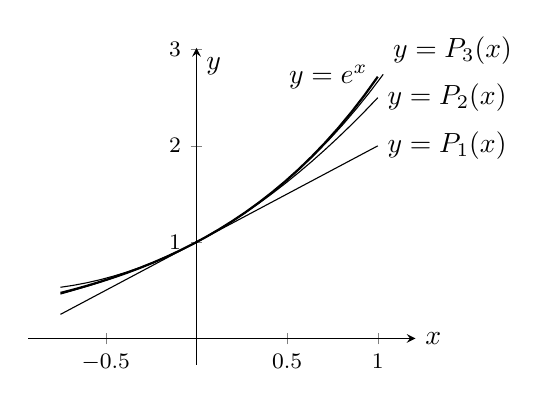
\begin{tikzpicture}[declare function={f(\x)=e^(\x);fa(\x)=1+\x; fb(\x)=1+\x+1/2*\x^2;fc(\x)=1+\x+1/2*\x^2+1/6*\x^3;}]
\begin{axis}[clip=false,small,axis lines=middle,xlabel={$x$},ylabel={$y$},xlabel style={at={(current axis.right of origin)},anchor=west},ymin=0,enlargelimits=true]
\addplot[thick,domain=-0.75:1]{f(x)}node[left]{$y=e^x$};
\addplot[domain=-0.75:1]{fa(x)}node[right]{$y=P_1(x)$};
\addplot[domain=-0.75:1]{fb(x)}node[right]{$y=P_2(x)$};
\addplot[domain=-0.75:1.03]{fc(x)}node[above right]{$y=P_3(x)$};
\end{axis}
\end{tikzpicture}
\caption{قوت نمائی تفاعل \عددی{f(x)=e^x} کی ٹیلر کثیر رکنیاں (مثال \حوالہ{مثال_ٹیلر_کثیر_رکنیاں_قوت_نمائی})}
\label{شکل_مثال_ٹیلر_کثیر_رکنیاں_قوت_نمائی}
\end{minipage}\hfill
\begin{minipage}{0.45\textwidth}
\centering
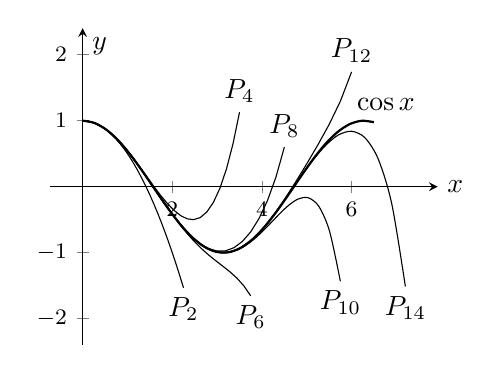
\begin{tikzpicture}[declare function={f(\x)=cos(deg(\x));fa(\x)=1-1/2*\x^2; fb(\x)=1-1/2*\x^2+1/24*\x^4;fc(\x)=fb(\x)-1/720*\x^6;fd(\x)=fc(\x)+1/40320*\x^8;fe(\x)=fd(\x)-1/3628800*\x^10;ff(\x)=fe(\x)+1/479001600*\x^12;fg(\x)=ff(\x)-1/87178291200*\x^14;}]
\begin{axis}[small,axis lines=middle,xlabel={$x$},ylabel={$y$},xlabel style={at={(current axis.right of origin)},anchor=west},enlargelimits=true,ymin=-2,ymax=2]
\addplot[thick,smooth,domain=0:6.5]{f(x)}node[shift={(1ex,1.5ex)}]{$\cos x$};
\addplot[domain=0:2.25]{fa(x)}node[below]{$P_2$};
\addplot[domain=0:3.5]{fb(x)}node[above]{$P_4$};
\addplot[domain=0:3.75]{fc(x)}node[below]{$P_6$};
\addplot[domain=0:4.5]{fd(x)}node[above]{$P_8$};
\addplot[smooth,domain=0:5.75]{fe(x)}node[below]{$P_{10}$};
\addplot[domain=0:6]{ff(x)}node[above]{$P_{12}$};
\addplot[smooth,domain=0:7.2]{fg(x)}node[below]{$P_{14}$};
\end{axis}
\end{tikzpicture}
\caption{کوسائن اور اس کی ٹیلر کثیر رکنیاں (مثال \حوالہ{مثال_تسلسل_کوسائن_ٹیلر_کثیر_رکنیاں})}
\label{شکل_مثال_تسلسل_کوسائن_ٹیلر_کثیر_رکنیاں}
\end{minipage}
\end{figure}

%===================
\ابتدا{مثال}\شناخت{مثال_تسلسل_کوسائن_ٹیلر_کثیر_رکنیاں}
نقطہ \عددی{x=0} پر تفاعل \عددی{f(x)=\cos x} کا ٹیلر تسلسل اور ٹیلر کثیر رکنیاں حاصل کریں۔

حل:\quad
تفاعل اور اس کے تفرقات درج ذیل ہیں۔
\begin{align*}
f(x)&=\cos x&& f'(x)=-\sin x\\
f''(x)&=-\cos x&&f^{(3)}(x)=\sin x\\
\vdots&\\
f^{(2n)}(x)&=(-1)^n \cos x&&f^{(2n+1)}=(-1)^{n+1}\sin x
\end{align*}
نقطہ \عددی{0} پر کوسائن کی قیمتیں \عددی{1} جبکہ سائن کی قیمتیں \عددی{0} ہیں لہٰذا
\begin{align*}
f^{(2n)}(0)=(-1)^n,\quad f^{(2n+1)}(0)=0
\end{align*}
ہوں گے۔ نقطہ \عددی{0} پر \عددی{f} کا پیدا کردہ ٹیلر تسلسل درج ذیل ہو گا۔
\begin{align*}
f(0)+f'(0)x+\frac{f''(0)}{2!}x^2&+\frac{f'''(0)}{3!}x^3+\cdots+\frac{f^{(n)}(0)}{n!}x^n+\cdots\\
&=1+0\cdot x-\frac{x^2}{2!}+0\cdot x^3+\frac{x^4}{4!}+\cdots+(-1)^n\frac{x^{2n}}{(2n)!}+\cdots\\
&=\sum_{n=0}^{\infty}\frac{(-1)^n x^{2n}}{(2n)!}
\end{align*}
تعریف کی رو سے یہی \عددی{\cos x} کا مکلارن تسلسل بھی ہو گا۔ ہم حصہ \حوالہ{حصہ_تسلسل_ٹیلر_اور_اندازہ_خلل} میں دیکھیں گے کہ تمام \عددی{x} کے لئے یہ تسلسل \عددی{\cos x} کو مرکوز ہو گا۔

چونکہ \عددی{f^{(2n+1)}(0)=0} ہے لہٰذا \عددی{2n} اور \عددی{2n+1} رتبی ٹیلر کثیر رکنیاں ایک دوسرے جیسی ہوں گی:
\begin{align*}
P_{2n}(x)=P_{2n+1}(x)=1-\frac{x^2}{2!}+\frac{x^4}{4!}-\cdots+(-1)^n\frac{x^{2n}}{(2n)!}
\end{align*}
آپ شکل \حوالہ{شکل_مثال_تسلسل_کوسائن_ٹیلر_کثیر_رکنیاں} میں دیکھ سکتے ہیں کہ \عددی{x=0} کی پڑوس میں یہ کثیر رکنیاں \عددی{\cos x} کے کتنے قریب ہیں۔ چونکہ \عددی{y} محور کے لحاظ سے ترسیمات تشاکلی ہیں لہٰذا انہیں صرف \عددی{x\ge 0} کے لئے دکھایا گیا ہے۔ 

کثیر رکنیاں \عددی{P_{2n}(x)} کوسائن تفاعل پر \عددی{n\to\infty} کرنے سے مرکوز ہوتی ہیں۔ ہم \عددی{x=0} پر کوسائن اور اس کے تفرقات کی قیمتیں جانتے ہوئے کسی بھی فاصلہ پر \عددی{\cos x} کا رویہ جان سکتے ہیں۔
\انتہا{مثال}
%===========================

ایسے لامتناہی گنّا قابل تفرق تفاعل جنہیں صرف الگ تھلگ نقطوں پر ٹیلر تسلسل سے ظاہر کرنا ممکن ہوں حقیقتاً بہت کم پائے جاتے ہیں۔

\ابتدا{مثال}\شناخت{مثال_تسلسل_مرکوز_لیکن_تفاعل_کو_نہیں}\quad \ترچھا{ایک تفاعل \عددی{f(x)} جس کا ٹیلر تسلسل ہر \عددی{x} پر مرتکز ہے لیکن یہ تسلسل صرف \عددی{x=0} پر \عددی{f(x)} کو  مرتکز ہے۔}

یہ (کافی محنت کے بعد) دکھایا جا سکتا ہے کہ \عددی{x=0} پر
 \begin{align*}
f(x)=
\begin{cases}
0,&x=0\\
e^{-1/x^2},&x\ne 0
\end{cases}
\end{align*}
کا ہر رتبے کا تفرق پایا جاتا ہے اور تمام \عددی{n} کے لئے \عددی{f^{(n)}(0)=0} ہیں۔ اس کا مطلب ہوا کہ \عددی{x=0} پر \عددی{f} کا پیدا کردہ تسلسل
\begin{align*}
f(0)+f'(0)x+\frac{f''(0)}{2!}x^2+\cdots &+\frac{f^{(n)}(0)}{n!}+\cdots\\
&=0+0\cdot x+0\cdot x^2+\cdots+0\cdot x^n+\cdots\\
&=0+0+\cdots+0+\cdots
\end{align*}
ہو گا جو ہر \عددی{x} کے لئے مرتکز ہے (جس کا مجموعہ \عددی{0} ہے) لیکن یہ صرف \عددی{x=0} پر \عددی{f(x)} کو مرتکز ہے۔  تفاعل \عددی{y=e^{-1/x^2}} کی استمراری توسیع کا ترسیم (شکل \حوالہ{شکل_مثال_تسلسل_مرکوز_لیکن_تفاعل_کو_نہیں}) صفر پر اتنا (افقی) سیدھا ہے کہ اس کے تمام تفرقات یہاں \عددی{0} کے برابر ہیں۔
\انتہا{مثال}
%===================== 
\begin{figure}
\centering
\begin{tikzpicture}[declare function={f(\x)=e^(-1/\x^2);}]
\begin{axis}[clip=false,small,axis lines=middle, xlabel={$x$},ylabel={$y$},xlabel style={at={(current axis.right of origin)},anchor=west},ylabel style={at={(current axis.above origin)},anchor=south},ytick={1},enlargelimits=true]
\addplot[smooth,domain=0:0.5]{f(x)};
\addplot[smooth,domain=0.5:4.5]{f(x)};
\addplot[smooth,domain=0:0.5]({-x},{f(x)});
\addplot[smooth,domain=0.5:4.5](-x,{f(x)});
\addplot[] plot coordinates {(2,0.5)}node[right]{$y=\begin{cases}0,&x=0\\  e^{-1/x^2},&x\ne 0  \end{cases}$};
\end{axis}
\end{tikzpicture}
\caption{صفر پر تفاعل کا ترسیم اتنا (افقی) سیدھا ہے  کے یہاں اس کے تمام تفرقات \عددی{0} ہیں۔}
\label{شکل_مثال_تسلسل_مرکوز_لیکن_تفاعل_کو_نہیں}
\end{figure}


دو سوالات اب بھی رہتے ہیں۔
\begin{enumerate}[a.]
\item
ہم \عددی{x} کی کن قیمتوں کے لئے توقع کر سکتے ہیں کہ ایک تفاعل کا پیدا کردہ ٹیلر تسلسل اسی تفاعل پر مرتکز ہو گا؟
\item
کسی دیے گئے وقفہ پر ایک تفاعل  کا ٹیلر کثیر رکنی تخمین کتنی درستگی کے ساتھ اس تفاعل کو ظاہر کرتا ہے؟
\end{enumerate} 

ان سوالات کے جوابات اگلے حصہ میں ٹیلر کا ایک مسئلہ دیتا ہے۔


\حصہء{سوالات}
\موٹا{ٹیلر تسلسل کا حصول}\\
سوال \حوالہ{سوال_تسلسل_ٹیلر_کثیر_رکنی_حصول_الف} تا سوال \حوالہ{سوال_تسلسل_ٹیلر_کثیر_رکنی_حصول_ب} میں \عددی{a} پر \عددی{f} کے پیدا کردہ  \عددی{0}، \عددی{1}، \عددی{2} اور \عددی{3} رتبی  ٹیلر کثیر رکنی حاصل کریں۔  

\ابتدا{سوال}\شناخت{سوال_تسلسل_ٹیلر_کثیر_رکنی_حصول_الف}
$f(x)=\ln x,\quad a=1$\\
جواب:\quad
\عددی{P_0(x)=0}، \عددی{P_1(x)=x-1}، \عددی{P_2(x)=(x-1)-\tfrac{1}{2}(x-1)^2} \\
  \عددی{P_3(x)=(x-1)-\tfrac{1}{2}(x-1)^2+\tfrac{1}{3}(x-1)^3}
\انتہا{سوال}
%=========================
\ابتدا{سوال}
$f(x)=\ln(1+x),\quad a=0$
\انتہا{سوال}
%=========================
\ابتدا{سوال}
$f(x)=\frac{1}{x},\quad a=2$\\
جواب:\quad
\عددی{P_0(x)=\tfrac{1}{2}}، \عددی{P_1(x)=\tfrac{1}{2}-\tfrac{1}{4}(x-2)}، \عددی{P_2(x)=\tfrac{1}{2}-\tfrac{1}{4}(x-2)+\tfrac{1}{8}(x-2)^2}،\\ \عددی{P_3(x)=\tfrac{1}{2}-\tfrac{1}{4}(x-2)+\tfrac{1}{8}(x-2)^2-\tfrac{1}{16}(x-2)^3}
\انتہا{سوال}
%=========================
\ابتدا{سوال}
$f(x)=\frac{1}{x+2},\quad a=0$
\انتہا{سوال}
%=========================
\ابتدا{سوال}
$f(x)=\sin x,\quad a=\frac{\pi}{4}$\\
جواب:\quad
\عددی{P_0(x)=\tfrac{\sqrt{2}}{2}}، \عددی{P_1(x)=\tfrac{\sqrt{2}}{2}+\tfrac{\sqrt{2}}{2}(x-\tfrac{\pi}{4})}،\\ \عددی{P_2(x)=\tfrac{\sqrt{2}}{2}+\tfrac{\sqrt{2}}{2}(x-\tfrac{\pi}{4})-\tfrac{\sqrt{2}}{4}(x-\tfrac{\pi}{4})^2}، \\
\عددی{P_3(x)=\tfrac{\sqrt{2}}{2}+\tfrac{\sqrt{2}}{2}(x-\tfrac{\pi}{4})-\tfrac{\sqrt{2}}{4}(x-\tfrac{\pi}{4})^2-\tfrac{\sqrt{2}}{12}(x-\tfrac{\pi}{4})^3}
\انتہا{سوال}
%=========================
\ابتدا{سوال}
$f(x)=\cos x,\quad a=\frac{\pi}{4}$
\انتہا{سوال}
%=========================
\ابتدا{سوال}
$f(x)=\sqrt{x},\quad a=4$\\
جواب:\quad
\عددی{P_0(x)=2}،\عددی{P_1(x)=2+\tfrac{1}{4}(x-4)}،\\ \عددی{P_2(x)=2+\tfrac{1}{4}(x-4)-\tfrac{1}{64}(x-4)^2}، \\
\عددی{P_3(x)=2+\tfrac{1}{4}(x-4)-\tfrac{1}{64}(x-4)^2+\tfrac{1}{512}(x-4)^3}
\انتہا{سوال}
%=========================
\ابتدا{سوال}\شناخت{سوال_تسلسل_ٹیلر_کثیر_رکنی_حصول_ب}
$f(x)=\sqrt{x+4},\quad a=0$
\انتہا{سوال}
%=========================
\موٹا{مکلارن تسلسل کا حصول}\\
سوال \حوالہ{سوال_تسلسل_مکلارن_حصول_الف} تا سوال \حوالہ{سوال_تسلسل_مکلارن_حصول_ب} میں دیے گئے تفاعل کا مکلارن تسلسل تلاش کریں۔

\ابتدا{سوال}\شناخت{سوال_تسلسل_مکلارن_حصول_الف}
$e^{-x}$\\
جواب:\quad
$\sum\limits_{n=0}^{\infty}\tfrac{(-x)^n}{n!}=1-x+\tfrac{x^2}{2!}-\tfrac{x^3}{3!}+\tfrac{x^4}{4!}-\cdots$
\انتہا{سوال}
%=====================
\ابتدا{سوال}
$e^{x/2}$
\انتہا{سوال}
%=====================
\ابتدا{سوال}
$\frac{1}{1+x}$\\
جواب:\quad
$\sum\limits_{n=0}^{\infty}(-1)^nx^n=1-x+x^2-x^3+\cdots$
\انتہا{سوال}
%=====================
\ابتدا{سوال}
$\frac{1}{1-x}$
\انتہا{سوال}
%=====================
\ابتدا{سوال}
$\sin 3x$\\
جواب:\quad
$\sum\limits_{n=0}^{\infty}\tfrac{(-1)^n3^{2n+1}x^{2n+1}}{(2n+1)!}$
\انتہا{سوال}
%=====================
\ابتدا{سوال}
$\sin \frac{x}{2}$
\انتہا{سوال}
%=====================
\ابتدا{سوال}
$7\cos (-x)$\\
جواب:\quad
$7\sum\limits_{n=0}^{\infty}\tfrac{(-1)^nx^{2n}}{(2n)!}$
\انتہا{سوال}
%=====================
\ابتدا{سوال}
$5\cos \pi x$
\انتہا{سوال}
%=====================
\ابتدا{سوال}
$\cosh x=\frac{e^x+e^{-x}}{2}$\\
جواب:\quad
$\sum\limits_{n=0}^{\infty}\tfrac{x^{2n}}{(2n)!}$
\انتہا{سوال}
%=====================
\ابتدا{سوال}
$\sinh x=\frac{e^x-e^{-x}}{2}$
\انتہا{سوال}
%=====================
\ابتدا{سوال}
$x^4-2x^3-5x+4$\\
جواب:\quad
$x^4-2x^3-5x+4$
\انتہا{سوال}
%=====================
\ابتدا{سوال}\شناخت{سوال_تسلسل_مکلارن_حصول_ب}
$(x+1)^2$
\انتہا{سوال}
%=====================
\موٹا{ٹیلر تسلسل کی تلاش}\\
سوال \حوالہ{سوال_تسلسل_ٹیلر_تسلسل_تلاش_الف} تا سوال \حوالہ{سوال_تسلسل_ٹیلر_تسلسل_تلاش_ب} میں \عددی{x=a} پر \عددی{f} کا پیدا کردہ ٹیلر تسلسل تلاش کریں۔

\ابتدا{سوال}\شناخت{سوال_تسلسل_ٹیلر_تسلسل_تلاش_الف}
$f(x)=x^3-2x+4,\quad a=2$\\
جواب:\quad
$8+10(x-2)+6(x-2)^2+(x-2)^3$
\انتہا{سوال}
%======================
\ابتدا{سوال}
$f(x)=2x^3+x^2+3x-8,\quad a=1$
\انتہا{سوال}
%======================
\ابتدا{سوال}
$f(x)=x^4+x^2+1,\quad a=-2$\\
جواب:\quad
$21-36(x+2)+25(x+2)^2-8(x+2)^3+(x+2)^4$
\انتہا{سوال}
%======================
\ابتدا{سوال}
$f(x)=3x^5-x^4+2x^3+x^2-2,\quad a=-1$
\انتہا{سوال}
%======================
\ابتدا{سوال}
$f(x)=\frac{1}{x^2},\quad a=1$\\
جواب:\quad
$\sum\limits_{n=0}^{\infty}(-1)^n(n+1)(x-1)^n$
\انتہا{سوال}
%======================
\ابتدا{سوال}
$f(x)=\frac{x}{1-x},\quad a=0$
\انتہا{سوال}
%======================
\ابتدا{سوال}
$f(x)=e^x,\quad a=2$\\
جواب:\quad
$\sum\limits_{n=0}^{\infty}\tfrac{e^2}{n!}(x-2)^n$
\انتہا{سوال}
%======================
\ابتدا{سوال}\شناخت{سوال_تسلسل_ٹیلر_تسلسل_تلاش_ب}
$f(x)=2^x,\quad a=1$
\انتہا{سوال}
%======================
\موٹا{نظریہ اور مثالیں}\\
\ابتدا{سوال}\شناخت{سوال_ٹیلر_نظریہ_الف}
نقطہ \عددی{x=a} پر \عددی{e^x} کا پیدا کردہ تسلسل استعمال کرتے ہوئے درج ذیل دکھائیں۔
\begin{align*} 
e^x=e^a[1+(x-a)+\frac{(x-a)^2}{2!}+\cdots]
\end{align*}
\انتہا{سوال}
%====================
\ابتدا{سوال}
نقطہ \عددی{x=1} پر \عددی{e^x} کا پیدا کردہ ٹیلر تسلسل تلاش کریں۔  سوال \حوالہ{سوال_ٹیلر_نظریہ_الف}  میں حاصل کلیہ کے ساتھ اپنے جواب کا موازنہ کریں۔
\انتہا{سوال}
%=====================
\ابتدا{سوال}
فرض کریں \عددی{x=a} پر \عددی{f(x)} کے \عددی{n} رتبہ تک تمام تفرقات پائے جاتے ہوں۔ دکھائیں کہ \عددی{x=a} پر \عددی{n} رتبی ٹیلر کثیر رکنی اور اس کے ابتدائی \عددی{n} تفرقات کی قیمتیں وہیں ہیں جو \عددی{x=a} پر \عددی{f} اور اس کے ابتدائی \عددی{n} تفرقات کی قیمتیں ہیں۔ 
\انتہا{سوال}
%=======================
\ابتدا{سوال}
\ترچھا{درجہ \عددی{\le n} کے تمام کثیر رکنیوں میں سب سے بہتر تخمین \عددی{n} رتبی کثیر رکنی دیتی ہے۔} فرض کریں \عددی{f(x)} ایک وقفہ  جس کا مرکز \عددی{x=a} ہو پر قابل تفرق ہے اور \عددی{g(x)=b_0+b_1(x-a)+\cdots+b_n(x-a)^n} ایک کثیر رکنی ہے جس کا درجہ \عددی{n}  اور جس کے عددی سر مستقل \عددی{b_0}، \نقطے، \عددی{b_n} ہیں۔فرج کریں \عددی{E(x)=f(x)-g(x)} ہے۔ دکھائیں کہ \عددی{g} پر درج ذیل شرائط
\begin{enumerate}[a.]
\item
$E(a)=0$\quad\quad
نقطہ \عددی{x=a} پر تخمینی خلل صفر ہے۔
\item
$\lim\limits_{x\to a}\frac{E(x)}{(x-a)^n}=0$\quad\quad
\عددی{(x-a)^n} کے لحاظ سے خلل قابل نظر انداز ہے۔
\end{enumerate}
 لاگو کرنے سے درج ذیل حاصل ہوتا ہے۔
\begin{align*}
g(x)=f(a)+f'(a)(x-a)+\frac{f''(a)}{2!}(x-a)^2+\cdots+\frac{f^{(n)}(a)}{n!}(x-a)^n
\end{align*}
یوں \عددی{P_n(x)} وہ واحد \عددی{n} کے برابر یا اس سے کم درجہ کی کثیر رکنی ہے جس کا خلل \عددی{x=a} پر صفر اور \عددی{(x-a)^n} کے لحاظ سے قابل نظر انداز ہے۔ 
\انتہا{سوال}
%======================
\موٹا{دو درجی تخمینات}\\
نقطہ \عددی{x=a} پر دو گنّا قابل تفرق تفاعل \عددی{f(x)} کی پیدا کردہ \عددی{2} رتبی ٹیلر کثیر رکنی کو \عددی{x=a} پر \عددی{f} کی \اصطلاح{دو درجی تخمین}\فرہنگ{دو درجی!تخمین}\حاشیہب{quadratic approximation}\فرہنگ{quadratic!approximation} کہتے ہیں۔ سوال \حوالہ{سوال_دو_قدری_الف} تا سوال \حوالہ{سوال_دو_قدری_ب} میں \عددی{x=0} پر \عددی{f} کی (الف) خط بندی (\عددی{1} رتبی ٹیلر کثیر رکنی) اور (ب) دو درجی تخمین تلاش کریں۔

\ابتدا{سوال}\شناخت{سوال_دو_قدری_الف}
$f(x)=\ln(\cos x)$\\
جواب:\quad
$L(x)=0,\, Q(x)=-\tfrac{x^2}{2}$
\انتہا{سوال}
%====================
\ابتدا{سوال}
$f(x)=e^{\sin x}$
\انتہا{سوال}
%====================
\ابتدا{سوال}
$f(x)=\frac{1}{\sqrt{1-x^2}}$\\
جواب:\quad
$L(x)=1,\, Q(x)=1+\tfrac{x^2}{2}$
\انتہا{سوال}
%====================
\ابتدا{سوال}
$f(x)=\cosh x$
\انتہا{سوال}
%====================
\ابتدا{سوال}
$f(x)=\sin x$\\
جواب:\quad
$L(x)=x,\, Q(x)=x$
\انتہا{سوال}
%====================
\ابتدا{سوال}\شناخت{سوال_دو_قدری_ب}
$f(x)=\tan x$
\انتہا{سوال}
%====================


\حصہ{ٹیلر تسلسل کا ارتکاز؛ خلل کے اندازے}\شناخت{حصہ_تسلسل_ٹیلر_اور_اندازہ_خلل}
اس حصہ میں ان دو سوالات کا جواب دیا جائے گا جن کے جوابات حصہ \حوالہ{حصہ_تسلسل_ٹیلر_مکلارن_تسلسل} میں نہیں دیے گئے۔
\begin{enumerate}[a.]
\item
کب ایک ٹیلر تسلسل اپنے پیدا کردہ تفاعل پر مرکوز ہو گا؟
\item
کسی بھی وقفہ پر ایک تفاعل کے ٹیلر کثیر رکنیاں اس تفاعل کی کتنی درست تخمین دیتی ہیں؟
\end{enumerate}

\ابتدا{مسئلہ}\شناخت{مسئلہ_تسلسل_ٹیلر_مسئلہ}\\
\موٹا{مسئلہ ٹیلر}\\
اگر \عددی{[a,b]} یا \عددی{[b,a]} پر \عددی{f} اور اس کے \عددی{n} تفرقات \عددی{f'}، \عددی{f''}، \نقطے، \عددی{f^{(n)}} استمراری ہوں اور \عددی{(a,b)} یا \عددی{(b,a)} پر \عددی{f^{(n)}} قابل تفرق ہو تب \عددی{a} اور \عددی{b} کے بیچ ایک ایسا عدد \عددی{c} موجود ہو گا جو درج ذیل کو مطمئن کرتا ہو۔
\begin{multline*}
f(b)=f(a)+f'(a)(b-a)+\frac{f''(a)}{2!}(b-a)^2+\cdots\\
+\frac{f^{(n)}(a)}{n!}(b-a)^n+\frac{f^{(n+1)}(c)}{(n+1)!}(b-a)^{n+1}
\end{multline*}
\انتہا{مسئلہ}
%==========================

مسئلہ ٹیلر درحقیقت مسئلہ اوسط قیمت کی عمومی شکل ہے (سوال \حوالہ{سوال_لامتاہی_تسلسل_ٹیلر_اور_مسئلہ_اوسط_قیمت})۔ 
مسئلہ اوسط قیمت کی عمومی صورت مسئلہ ٹیلر ہے۔ اس حصہ کے آخر میں مسئلہ ٹیلر کا ثبوت پیش کیا گیا ہے۔

مسئلہ ٹیلر کو استعمال کرتے ہوئے ہم عموماً \عددی{a} کو مستقل جبکہ \عددی{b} کو غیر تابع متغیر رکھنا چاہتے ہیں۔ ایسی صورتوں میں ہم \عددی{b} کی جگہ \عددی{x} پر کرتے ہیں۔ اس تبدیلی کے بعد یہ مسئلہ درج ذیل پڑھا جائے گا۔

\ابتدا{ضمنی نتیجہ} مسئلہ ٹیلر کا ضمنی نتیجہ\\
\موٹا{مسئلہ ٹیلر}\\
اگر وقفہ \عددی{I}، جس میں \عددی{a} پایا جاتا ہو، میں \عددی{f} کے ہر رتبی تفرقات پائے جاتے ہوں، تب ہر مثبت عدد صحیح \عددی{n} اور \عددی{I} میں ہر \عددی{x} کے لئے
\begin{multline}\label{مساوات_تسلسل_ٹیلر_ضمنی_نتیجہ_الف}
f(x)=f(a)+f'(a)(x-a)+\frac{f''(a)}{2!}(x-a)^2+\cdots\\
+\frac{f^{(n)}(a)}{n!}(x-a)^n+R_n(x)
\end{multline}
ہو گا جہاں 
\begin{align}\label{مساوات_تسلسل_ٹیلر_ضمنی_نتیجہ_ب}
R_n(x)=\frac{f^{(n+1)}(c)}{(n+1)!}(x-a)^{n+1}
\end{align}
ہے جبکہ \عددی{a} اور \عددی{x} کے بیچ \عددی{c} کوئی نقطہ ہے۔
\انتہا{ضمنی نتیجہ}
%=================

مسئلہ ٹیلر کو اس طرح بیان کرنے سے یہ کہتا ہے کہ \عددی{I} میں ہر \عددی{x} کے لئے درج ذیل ہو گا۔
\begin{align*}
f(x)=P_n(x)+R_n(x)
\end{align*}
ذرہ رک کر اس قابل ذکر مساوات پر غور کریں۔ یہ کلیہ وقفہ \عددی{I} پر کسی بھی \عددی{n} کے لئے \عددی{f} کی اسی رتبے کی تخمینی کثیر رکنی دیتی ہے اور اس تخمین سے پیدا خلل کا کلیہ بھی دیتی ہے۔ 

مساوات \حوالہ{مساوات_تسلسل_ٹیلر_ضمنی_نتیجہ_الف} کو \اصطلاح{کلیہ ٹیلر}\فرہنگ{ٹیلر!کلیہ}\حاشیہب{Taylor's formula}\فرہنگ{Taylor's!formula} کہتے ہیں۔ تفاعل \عددی{R_n(x)} کو وقفہ \عددی{I} پر \عددی{f} کی تخمین \عددی{P_n(x)} کا \اصطلاح{\عددی{n} رتبی باقی} یا \اصطلاح{جزو خلل} کہتے ہیں۔ اگر \عددی{I} میں تمام \عددی{x} کے لئے \عددی{n\to \infty}  سے \عددی{R_n(x)\to 0} حاصل ہو تب ہم کہتے ہیں کہ \عددی{x=a} پر \عددی{f} کا پیدا کردہ ٹیلر تسلسل \عددی{I} پر \عددی{f} کو مرکوز ہے جس کو درج ذیل لکھا جاتا ہے۔
\begin{align*}
f(x)=\sum_{k=0}^{\infty}\frac{f^{(k)}(a)}{k!}(x-a)^k
\end{align*}

\ابتدا{مثال}\شناخت{مثال_تسلسل_قوت_نمائی_تسلسل_باقی} \ترچھا{تفاعل \عددی{e^x} کا مکلارن تسلسل}\\
دکھائیں کہ  \عددی{x=0} پر \عددی{f(x)=e^x} کا پیدا کردہ ٹیلر تسلسل ہر حقیقی \عددی{x} کے لئے \عددی{f} کو مرکوز ہے۔

حل: \quad
تمام وقفہ \عددی{(-\infty,\infty)} میں اس تفاعل کے ہر رتبی تفرقات پائے جاتے ہیں۔  مساوات \حوالہ{مساوات_تسلسل_ٹیلر_ضمنی_نتیجہ_الف} اور مساوات \حوالہ{مساوات_تسلسل_ٹیلر_ضمنی_نتیجہ_ب} تفاعل \عددی{f(x)=e^x} اور \عددی{a=0} لیتے ہوئے
\begin{align*}
e^x&=1+x+\frac{x^2}{2!}+\cdots+\frac{x^n}{n!}+R_n(x)&&\text{\RL{(مثال \حوالہ{مثال_ٹیلر_کثیر_رکنیاں_قوت_نمائی})}}
\end{align*}
اور
\begin{align*}
R_n(x)&=\frac{e^{\,c}}{(n+1)!}x^{n+1}&&\text{\RL{\scriptsize{\عددی{0} اور \عددی{x} کے بیچ کسی \عددی{c} کے لئے}}}
\end{align*}
دیتے ہیں۔ چونکہ \عددی{e^x} متغیر \عددی{x} کے ساتھ بڑھتا تفاعل ہے، لہٰذا \عددی{e^0=1} اور \عددی{e^x} کے بیچ \عددی{e^c} پایا جائے گا۔ جب \عددی{x} منفی ہو تب \عددی{c} بھی منفی اور \عددی{e^c<1} ہو گا۔ جب \عددی{x} صفر ہو تب \عددی{e^x=1} اور \عددی{R_n(x)=0} ہو گا۔ جب \عددی{x} مثبت ہو تب \عددی{c} بھی مثبت اور \عددی{e^c<e^x} ہو گا۔یوں
\begin{align*}
\abs{R_n(x)}&\le \frac{\abs{x}^{n+1}}{(n+1)!}&&x\le 0
\end{align*} 
اور
\begin{align*}
\abs{R_n(x)}&<e^x\frac{x^{n+1}}{(n+1)!}&x>0
\end{align*}
ہوں گے۔ آخر میں، چونکہ تمام \عددی{x} کے لئے
\begin{align*}
\lim_{n\to\infty}\frac{x^{n+1}}{(n+1)!}&=0&&  \text{\RL{(حصہ \حوالہ{حصہ_ترتیب_حد_تلاش_کے_مسائل})}}
\end{align*}
ہے لہٰذا \عددی{\lim\limits_{n\to\infty}R_n(x)=0} ہو گا اور تمام \عددی{x} کے لئے یہ تسلسل \عددی{e^x} کو مرکوز ہو گا۔
\begin{align*}
e^x=\sum_{k=0}^{\infty}\frac{x^k}{k!}=1+x+\frac{x^2}{2!}+\cdots+\frac{x^k}{k!}+\cdots
\end{align*}
\انتہا{مثال}
%==================

\جزوحصہء{باقی کا اندازہ}
عموماً  \عددی{R_n(x)} کا اندازہ مثال \حوالہ{مثال_تسلسل_قوت_نمائی_تسلسل_باقی} کی طرح  لگایا جا سکتا ہے۔اندازہ لگانے کی یہ ترکیب اتنی آسان ہے کہ مستقل میں استعمال کرنے کی غرض سے ہم اس کو بطور ایک مسئلہ بیان کرتے ہیں۔ 

\ابتدا{مسئلہ} \موٹا{مسئلہ اندازہ باقی}\\
اگر ایسے مثبت مستقل \عددی{M} اور \عددی{r} ہوں کہ \عددی{a} اور \عددی{x} کے بشمول اور ان کے بیچ تمام \عددی{t} کے لئے \عددی{\abs{f^{(n+1)}(t)}\le Mr^{n+1}} ہو تب مسئلہ ٹیلر میں جزو باقی درج ذیل عدم مساوات کو مطمئن کرے گا۔
\begin{align*}
\abs{R_n(x)}\le M\,\frac{r^{n+1}\abs{x-a}^{n+1}}{(n+1)!}
\end{align*}
اگر یہ شرائط تمام \عددی{n} کے لئے مطمئن ہوں اور  مسئلہ ٹیلر کے باقی تمام شرائط کو \عددی{f} مطمئن کرتا ہو تب یہ تسلسل \عددی{f(x)} کو مرکوز ہو گا۔
\انتہا{مسئلہ}
%=======================

سادہ ترین مثال میں ہم \عددی{r=1} لے سکتے ہیں بشرطیکہ \عددی{f} اور اس کے تفرقات کی مقدار کا حد کوئی مستقل \عددی{M} ہو۔ دیگر صورتوں میں ہمیں \عددی{r} کو بھی لینا ہو گا۔ مثال کے طور پر اگر \عددی{f(x)=2\cos (3x)} ہو تب ہر تفرق جزو ضربی \عددی{3} دیگا لہٰذا \عددی{r} کو \عددی{1} سے بڑا منتخب کرنا لازمی ہو گا۔ اس مخصوص مثال میں ہم \عددی{r=3} اور \عددی{M=2} منتخب کر سکتے ہیں۔

مسئلہ اندازہ باقی اور  مسئلہ ٹیلر استعمال کرتے ہوئے ہم اب ارتکاز کے مسائل حل کر سکتے ہیں۔ جیسا آپ دیکھیں گے، ہم ان سے کسی تفاعل کو تخمیناً ٹیلر کثیر رکنی سے ظاہر کرنے کی درستگی بھی جان سکتے ہیں۔

\ابتدا{مثال}\ترچھا{تفاعل \عددی{\sin x} کا مکلارن تسلسل}\\
دکھائیں کہ تمام \عددی{x} کے لئے \عددی{\sin x} کا مکلارن تسلسل \عددی{\sin x} کو مرکوز ہے۔

حل:\quad
تفاعل اور اس کے تفرقات
\begin{align*}
f(x)&=\sin x,&&f'(x)=\cos x\\
f''(x)&=-\sin x,&&f'''(x)=-\cos x\\
\vdots&\\
f^{(2k)}(x)&=(-1)^k\sin x,&&f^{(2k+1)}(x)=(-1)^k\cos x
\end{align*}
ہیں لہٰذا
\begin{align*}
f^{(2k)}(0)&=0&&f^{(2k+1)}(0)=(-1)^k
\end{align*}
ہوں گے۔ تسلسل میں صرف طاق طاقتی اجزاء پائے جائیں گے اور \عددی{n=2k+1} کے لئے مسئلہ ٹیلر کے تحت درج ذیل ہو گا۔
\begin{align*}
\sin x=x-\frac{x^3}{3!}+\frac{x^5}{5!}-\cdots+\frac{(-1)^kx^{2k+1}}{(2k+1)!}+R_{2k+1}(x)
\end{align*}
تفاعل \عددی{\sin x} کے تمام تفرقات کی مطلق قیمتیں \عددی{1} یا اس سے کم ہیں لہٰذا ہم اندازہ باقی کے مسئلہ میں \عددی{M=1} اور \عددی{r=1} لیتے ہوئے درج ذیل حاصل کرتے ہیں۔
\begin{align*}
\abs{R_{2k+1}(x)}\le 1\cdot\frac{\abs{x}^{2k+2}}{(2k+2)!}
\end{align*} 
چونکہ کسی بھی \عددی{x} کے لئے \عددی{k\to 0} سے \عددی{(\abs{x}^{2k+2}/(2k+2))\to 0} حاصل ہوتا ہے لہٰذا \عددی{R_{2k+1}(x)\to 0} ہو گا ور تمام \عددی{x} کے لئے \عددی{\sin x} کا مکلارن تسلسل \عددی{\sin x} کو مرکوز ہو گا۔
\begin{align}
\sin x=\sum_{k=0}^{\infty}\frac{(-1)^kx^{2k+1}}{(2k+1)!}=x-\frac{x^3}{3!}+\frac{x^5}{5!}-\frac{x^7}{7!}+\cdots
\end{align}
\انتہا{مثال}
%======================
\ابتدا{مثال}\ترچھا{تفاعل \عددی{\cos x} کا مکلارن تسلسل}\\
دکھائیں کہ تمام \عددی{x} کے لئے \عددی{\cos x} کا مکلارن تسلسل \عددی{\cos x} کو مرکوز ہے۔

حل:\quad ہم مثال \حوالہ{مثال_تسلسل_کوسائن_ٹیلر_کثیر_رکنیاں} میں حاصل \عددی{\cos x} کی کثیر رکنی کے ساتھ جزو باقی جمع کر کے \عددی{\cos x} کا کلیہ ٹیلر حاصل کرتے ہیں جس میں \عددی{n=2k} ہو گا:
\begin{align*}
\cos x=1-\frac{x^2}{2!}+\frac{x^4}{4!}-\cdots+(-1)^k\frac{x^{2k}}{(2k)!}+R_{2k}(x)
\end{align*}
چونکہ کوسائن کی مطلق قیمت \عددی{1} کے برابر یا اس سے کم ہوتی ہے لہٰذا اندازہ باقی کے مسئلہ \عددی{M=1} اور \عددی{r=1} کے ساتھ درج ذیل دیگا۔
\begin{align*}
\abs{R_{2k}(x)}\le 1\cdot \frac{\abs{x}^{2k+1}}{(2k+1)!}
\end{align*}
چونکہ \عددی{x} کی ہر قیمت کے لئے، \عددی{k\to \infty} سے \عددی{R_{2k}(x)\to 0} حاصل ہو گا لہٰذا ہر \عددی{x} کے لئے یہ تسلسل \عددی{\cos x} کو مرکوز ہو گا۔
\begin{align}\label{مساوات_تسلسل_کوسائن_مکلارن_الف}
\cos x=\sum_{k=0}^{\infty}\frac{(-1)^kx^{2k}}{(2k)!}=1-\frac{x^2}{2!}+\frac{x^4}{4!}-\frac{x^6}{6!}+\cdots
\end{align}
\انتہا{مثال}
%==================
\ابتدا{مثال}\شناخت{مثال_تسلسل_بدل_سے_مکلارن}\ترچھا{ترکیب بدل سے مکلارن تسلسل کا حصول}\\
تفاعل \عددی{\cos 2x} کا مکلارن تسلسل حاصل کریں۔

حل:\quad
ہم \عددی{\cos x} کے مکلارن تسلسل میں \عددی{x} کی جگہ \عددی{2x} پر کر کے \عددی{\cos 2x} کا تسلسل حاصل کیا جا سکتا ہے:
\begin{align*}
\cos 2x&=\sum_{k=0}^{\infty}\frac{(-1)^k(2x)^{2k}}{(2k)!}=1-\frac{(2x)^2}{2!}+\frac{(2x)^4}{4!}-\frac{(2x)^6}{6!}+\cdots && \text{\RL{\scriptsize{مساوات \حوالہ{مساوات_تسلسل_کوسائن_مکلارن_الف} میں \عددی{x} کی جگہ \عددی{2x}}}}\\
&=1-\frac{2^2x^2}{2!}+\frac{2^4x^4}{4!}-\frac{2^6x^6}{6!}+\cdots\\
&=\sum_{k=0}^{\infty}(-1)^k\,\frac{2^{2k}x^{2k}}{(2k)!}
\end{align*}   
وقفہ \عددی{-\infty<x<\infty} پر مساوات \حوالہ{مساوات_تسلسل_کوسائن_مکلارن_الف} مطمئن ہوتی ہے لہٰذا وقفہ \عددی{-\infty<2x<\infty} پر بھی یہ مطمئن ہو گی۔یوں نیا تسلسل تمام \عددی{x} کے لئے مرتکز ہو گا۔ سوال \حوالہ{سوال_لامتناہی_تسلسل_مسئلہ_اوسط_کی_عمومی} دکھاتا ہے کہ یہ تسلسل درحقیقت \عددی{\cos 2x} کا مکلارن تسلسل ہے۔
\انتہا{مثال}
%======================
\ابتدا{مثال}\ترچھا{مکلارن تسلسل کا حصول بذریعہ ضرب}\\
تفاعل \عددی{x\sin x} کا مکلارن تسلسل تلاش کریں۔

حل:\quad
ہم \عددی{\sin x} کے مکلارن تسلسل کو \عددی{x} سے ضرب دے کر \عددی{x\sin x} کا مکلارن تسلسل حاصل کر سکتے ہیں: 
\begin{align*}
x\sin x&=x\big(x-\frac{x^3}{3!}+\frac{x^5}{5!}-\frac{x^7}{7!}+\cdots\big)\\
&=x^2-\frac{x^4}{3!}+\frac{x^6}{5!}-\frac{x^8}{7!}+\cdots
\end{align*}
چونکہ \عددی{\sin x} کا تسلسل تمام \عددی{x} کے لئے مرتکز ہے لہٰذا یہ نیا تسلسل بھی تمام \عددی{x} کے لئے مرتکز ہو گا۔سوال \حوالہ{سوال_لامتناہی_تسلسل_مسئلہ_اوسط_کی_عمومی} دکھاتا ہے کہ یہ تسلسل درحقیقت \عددی{x\sin x} کا مکلارن تسلسل ہے۔
\انتہا{مثال}
%========================

\جزوحصہء{حذفی خلل}
 تمام \عددی{x} کے لئے \عددی{e^x} کا مکلارن تسلسل \عددی{e^x} کو مرکوز ہے۔ اس کے باوجود کسی مخصوص درستگی تک نتائج حاصل کرنے کے لئے درکار اجزاء کی تعداد جاننا ضروری ہو گا۔ مسئلہ اندازہ باقی ہمیں یہ معلومات فراہم کرتا ہے۔

\ابتدا{مثال}
\عددی{e} کی قیمت تلاش کریں جس میں خلل \عددی{10^{-6}} سے کم ہو۔

حل:\quad
ہم مثال \حوالہ{مثال_تسلسل_قوت_نمائی_تسلسل_باقی} کے نتیجہ میں \عددی{x=1}  لے کر
\begin{align*}
e=1+1+\frac{1}{2!}+\cdots+\frac{1}{n!}+R_n(1)
\end{align*}
لکھتے  ہیں جہاں \عددی{0} اور \عددی{1} کے بیچ کسی \عددی{c} پر درج ذیل ہو گا۔
\begin{align*}
R_n(1)=e^c\,\frac{1}{(n+1)!}
\end{align*}
اس مثال کے لئے ہم فرض کرتے ہیں کہ \عددی{e<3} ہے۔ چونکہ \عددی{0<c<1} کے لئے \عددی{1<e^c<3} ہے لہٰذا یقیناً درج ذیل ہو گا۔
\begin{align*}
\frac{1}{(n+1)!}<R_n(1)<\frac{3}{(n+1)!}
\end{align*}
تجربہ سے \عددی{\tfrac{1}{9!}>10^{-6}} اور \عددی{\tfrac{1}{10!}<10^{-6}} حاصل ہوتے ہیں لہٰذا ہمیں \عددی{(n+1)} کو کم از کم \عددی{10}، یا \عددی{n} کو کم از کم \عددی{9} لینا ہو گا۔خلل کو \عددی{10^{-6}} سے کم رکھتے ہوئے درج ذیل حاصل ہوتا ہے۔
\begin{align*}
e=1+1+\frac{1}{2!}+\frac{1}{3!}+\cdots+\frac{1}{9!}\approx \num{2.718282}
\end{align*}
\انتہا{مثال}
%===================
\ابتدا{مثال}\شناخت{مثال_تسلسل_سائن_کے_کثیر_رکنیاں_الف}
خلل کی مقدار کو \عددی{3\times 10^{-4}} سے کم رکھتے ہوئے ہم \عددی{x} کی کن قیمتوں کے لئے \عددی{\sin x} کو \عددی{x-\tfrac{x^3}{3!}} سے ظاہر کر سکتے ہیں؟

حل:\quad
ہر غیر صفر \عددی{x} کے لئے \عددی{\sin x} کا مکلارن تسلسل ایک بدلتا تسلسل ہے۔  مسئلہ بدلتے تسلسل کا اندازہ (مسئلہ  \حوالہ{مسئلہ_تسلسل_بدلتا_اندازہ}) کے تحت  
\begin{align*}
\sin x=x-\frac{x^3}{3!}\,\protect\rule[-2ex]{0.1ex}{5ex}+\frac{x^5}{5!}-\cdots
\end{align*}
کو \عددی{\tfrac{x^3}{3!}} کے بعد حذف کرنے سے خلل 
\begin{align*}
\abs{\frac{x^5}{5!}}=\frac{\abs{x}^5}{120}
\end{align*} 
 سے زیادہ نہیں ہو گا۔یوں اگر
\begin{align*}
\frac{\abs{x^5}}{120}<3\times 10^{-4}\quad \implies \quad \abs{x}<\sqrt[5]{360\times 10^{-4}}\approx 0.514\quad \text{\RL{\small{\begin{minipage}{0.15\textwidth}محفوظ رہنے کے لئے نیچے پور و پور  \end{minipage}}}}
\end{align*}
ہو تب خلل \عددی{3\times 10^{-4}} سے کم یا اس کے برابر ہو گا۔ مسئلہ بدلتے تسلسل کا اندازہ ہمیں وہ کچھ بتاتا ہے جو مسئلہ اندازہ باقی ہمیں نہیں بتاتا، یعنی، چونکہ مثبت \عددی{x} کے لئے \عددی{\tfrac{x^5}{120}} مثبت ہو گا لہٰذا \عددی{\sin x} کا اندازہ \عددی{x-\tfrac{x^3}{3!}} درحقیقت اصل قیمت سے کم ہو گا۔

شکل \حوالہ{شکل_مثال_تسلسل_سائن_کے_کثیر_رکنیاں_الف} میں \عددی{\sin x} اور اس کی کئی تخمینی ٹیلر کثیر رکنیاں دکھائی گئی ہیں۔ وقفہ \عددی{-1\le x\le 1} پر کثیر رکنی \عددی{P_3(x)=x-\tfrac{x^3}{3!}} اور تفاعل \عددی{\sin x} کے ترسیمات بالکل ایک دوسرے جیسے ہیں۔

آپ سوچ رہے ہوں گے کہ مسئلہ اندازہ باقی اور مسئلہ اندازہ بدلتا تسلسل کے نتائج میں سے کونسا اندازہ بہتر ہے۔ اگر ہم 
\begin{align*}
\sin x=x-\frac{x^3}{3!}+R_3
\end{align*}
لکھیں تب مسئلہ اندازہ باقی کے تحت
\begin{align*}
\abs{R_3}\le 1\cdot\frac{\abs{x}^4}{4!}=\frac{\abs{x}^4}{24}
\end{align*}
ہو گا جو اتنا بہتر نہیں ہے۔لیکن اگر ہم \عددی{x-\tfrac{x^3}{3!}=0+x+0x^2-\tfrac{x^3}{3!}+0x^4} لکھیں جو \عددی{3} رتبی اور \عددی{4} رتبی ٹیلر کثیر رکنی ہے تب
\begin{align*}
\sin x=x-\frac{x^3}{3!}+0+R_4
\end{align*}
لکھا جا سکتا ہے اور مسئلہ اندازہ باقی میں \عددی{M=r=1}  لیتے ہوئے 
\begin{align*}
\abs{R_4}\le 1\cdot \frac{\abs{x}^5}{5!}=\frac{\abs{x}^5}{120}
\end{align*}
حاصل ہو گا۔یہی نتیجہ مسئلہ اندازہ بدلتا تسلسل سے حاصل ہوتا ہے۔
\انتہا{مثال}
%====================
\begin{figure}
\centering
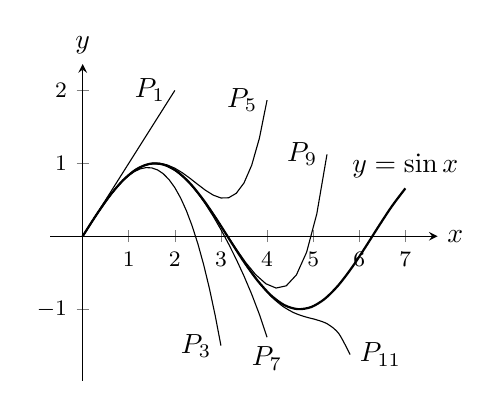
\begin{tikzpicture}[declare function={fa(\x)=\x;fb(\x)=fa(\x)-1/6*\x^3;fc(\x)=fb(\x)+1/120*\x^5;fd(\x)=fc(\x)-1/5040*\x^7;fe(\x)=fd(\x)+1/362880*\x^9;ff(\x)=fe(\x)-1/39916800*\x^11;}]
\begin{axis}[clip=false,small,axis lines=middle,enlargelimits=true,xlabel={$x$},ylabel={$y$},xlabel style={at={(current axis.right of origin)},anchor=west},ylabel style={at={(current axis.above origin)},anchor=south},xtick={1,2,3,4,5,6,7}]
\addplot[thick,smooth,domain=0:7]{sin(deg(x))}node[above]{$y=\sin x$};
\addplot[domain=0:2]{fa(x)}node[left]{$P_1$};
\addplot[domain=0:3]{fb(x)}node[left]{$P_3$};
\addplot[domain=0:4]{fc(x)}node[left]{$P_5$};
\addplot[domain=0:4]{fd(x)}node[below]{$P_7$};
\addplot[domain=0:5.3]{fe(x)}node[left]{$P_9$};
\addplot[smooth,domain=0:5.8]{ff(x)}node[right]{$P_{11}$};
\end{axis}
\end{tikzpicture}
\caption{\عددی{n\to \infty} کرنے سے کثیر رکنیاں \عددی{\sin x} پر مرکوز ہوتی ہیں}
\label{شکل_مثال_تسلسل_سائن_کے_کثیر_رکنیاں_الف}
\end{figure}

\جزوحصہء{ٹیلر تسلسلوں کا ملاپ}
ٹیلر تسلسلوں کے وقفات ارتکاز کے تقاطع پر، ٹیلر تسلسلوں کو  جمع، منفی اور مستقل سے ضرب دیا جا سکتا ہے۔ یوں حاصل تسلسل بھی ٹیلر تسلسل ہوں گے۔ تفاعل \عددی{f(x)+g(x)} کا ٹیلر تسلسل \عددی{f(x)} اور \عددی{g(x)} کے ٹیلر تسلسلوں کا مجموعہ ہو گا۔ اسی طرح \عددی{1} کے ساتھ \عددی{\cos 2x} کا مکلارن تسلسل جمع کر کے نتیجہ کو \عددی{2} سے تقسیم کرنے سے  \عددی{\tfrac{1+\cos 2x}{2}} کا مکلارن تسلسل حاصل ہو گا۔  \عددی{\sin x} اور \عددی{\cos x} کے مکلارن تسلسلوں کو جزو در جزو جمع کرنے سے \عددی{\sin x+\cos x} کا مکلارن تسلسل حاصل ہو گا۔  

\جزوحصہء{کلیہ یولر}
آپ جانتے ہیں کہ \عددی{a+ib} روپ کے عدد کو مخلوط عدد کہتے ہیں، جہاں \عددی{a} اور \عددی{b} مستقل ہیں جبکہ \عددی{i=\sqrt{-1}} ہے۔ اگر ہم \عددی{e^x} کے مکلارن تسلسل میں  \عددی{x=i\theta} پر کریں، جہاں \عددی{\theta} حقیقی ہو، اور درج ذیل تعلقات استعمال کریں
\begin{align*}
i^2=-1,\quad i^3=i^2i=-i,\quad i^2=i^2i^2=1,\quad i^5=i^4i=i,\quad \cdots
\end{align*}
تب درج ذیل حاصل ہو گا۔
\begin{align*}
e^{i\theta}&=1+\frac{i\theta}{1!}+\frac{i^2\theta^2}{2!}+\frac{i^3\theta^3}{3!}+\frac{i^4\theta^4}{4!}+\frac{i^5\theta^5}{5!}+\frac{i^6\theta^6}{6!}+\cdots\\
&=\big(1-\frac{\theta^2}{2!}+\frac{\theta^4}{4!}-\frac{\theta^6}{6!}+\cdots\big)+i\big(\theta-\frac{\theta^3}{3!}+\frac{\theta^5}{5!}-\cdots\big)\\
&=\cos \theta+i\sin \theta
\end{align*}
چونکہ ہم \عددی{e} کے خیالی طاقت کی تعریف نہیں جانتے ہیں لہٰذا درج بالا مساوات \عددی{e^{i\theta}=\cos \theta+i\sin\theta} کو ثابت نہیں کرتا ہے۔ البتہ یہ مساوات ہمیں \عددی{e^{i\theta}} کی ایسی تعریف پیش کرنے کا طریقہ دیتی ہے جو باقی ان تمام چیزوں کے ساتھ مطابقت رکھتی ہو جنہیں ہم جانتے ہیں۔

\ابتدا{تعریف}
کسی بھی حقیقی عدد \عددی{\theta} کے لئے درج ذیل ہو گا۔
\begin{align}\label{مساوات_تسلسل_کلیہ_یولر_الف}
e^{i\theta}=\cos \theta+i\sin\theta
\end{align}
\انتہا{تعریف}
%==========================

مساوات \حوالہ{مساوات_تسلسل_کلیہ_یولر_الف} جو \اصطلاح{کلیہ یولر}\فرہنگ{یولر!کلیہ}\حاشیہب{Euler's formula}\فرہنگ{Euler's!formula} کہلاتی ہے، کسی بھی مخلوط عدد \عددی{a+ib} کے لئے  ہمیں \عددی{e^{a+ib}} کی تعریف \عددی{e^a\cdot e^{ib}} دیتی ہے۔ 

\جزوحصہء{مسئلہ ٹیلر کا ثبوت}
ہم \عددی{a<b} فرض کرتے ہوئے مسئلہ ٹیلر ثابت کرتے ہیں۔ (\عددی{a>b} کے لئے بھی ثبوت تقریباً ایسا ہے۔)

نقطہ \عددی{x=a} پر ٹیلر کثیر رکنی
\begin{align*}
P_n(x)=f(a)+f'(a)(x-a)+\frac{f''(a)}{2!}(x-a)^2+\cdots+\frac{f^{(n)}(a)}{n!}(x-a)^n
\end{align*}
اور اس کے ابتدائی \عددی{n} تفرقات، تفاعل \عددی{f} اور اس کے ابتدائی \عددی{n} تفرقات کے موافق ہیں۔ اس میں \عددی{K(x-a)^{n+1}} طرز کا جزو، جہاں \عددی{K} مستقل ہے، شامل کرنے سے یہ موافقت خراب نہیں ہوتی ہے چونکہ  \عددی{x=a} پر ایسا جزو اور اس کے تمام تفرقات صفر ہیں۔نقطہ \عددی{x=a} پر یہ نیا تفاعل
\begin{align*}
\phi_n(x)=P_n(x)+K(x-a)^{n+1}
\end{align*}
اور اس کے ابتدائی \عددی{n} تفرقات، \عددی{f} اور اس کے ابتدائی \عددی{n} تفرقات کے ساتھ موافقت رکھیں گے۔

ہم ایسا \عددی{K}  منتخب کرتے ہیں کہ \عددی{x=b} پر \عددی{y=\phi_n(x)} کی منحنی اور اصل تفاعل \عددی{y=f(x)} کی منحنی ایک دوسری جیسی ہوں، یعنی:
\begin{align}\label{مساوات_تسلسل_کے_کی_قیمت}
f(b)=P_n(b)+K(b-a)^{n+1}\quad \implies \quad K=\frac{f(b)-P_n(b)}{(b-a)^{n+1}}
\end{align}
جب \عددی{K} کی قیمت مساوات \حوالہ{مساوات_تسلسل_کے_کی_قیمت} دیتی ہو تب وقفہ \عددی{[a,b]} میں تمام \عددی{x} کے لئے اصل تفاعل \عددی{f} اور تخمینی تفاعل \عددی{\phi_n} میں فرق درج ذیل تفاعل دیگا۔
\begin{align*}
F(x)=f(x)-\phi_n(x)
\end{align*}

ہم اب مسئلہ رول (حصہ \حوالہ{حصہ_استعمال_مسئلہ_اوسط_قیمت}) استعمال کرتے ہیں۔پہلی بات، چونکہ \عددی{F(a)=F(b)=0} ہے اور \عددی{[a,b]} پر \عددی{F} اور \عددی{F'} استمراری ہیں، ہم جانتے ہیں کہ 
\begin{align*}
F'(c_1)&=0&&\text{\RL{\عددی{(a,b)} میں کسی \عددی{c_1} پر}}
\end{align*}
ہو گا۔ دوسری بات، چونکہ \عددی{F'(a)=F'(c_1)=0} ہے اور ساتھ ہی \عددی{F'} اور \عددی{F''} دونوں \عددی{[a,c_1]} پر استمراری ہیں، ہم جانتے ہیں کہ 
\begin{align*}
F''(c_2)&=0&&\text{\RL{\عددی{(a,c_1)} میں کسی \عددی{c_2} پر}}
\end{align*}
ہو گا۔یک بعد دیگرے \عددی{F''}، \عددی{F'''}، \نقطے، \عددی{F^{(n-1)}} پر مسئلہ رول کی اطلاق سے درج ذیل مراد لیا جا سکتا ہے۔
\begin{align*}
\text{\RL{\عددی{(a,c_2)} میں ایسا \عددی{c_3} کہ \عددی{F'''(c_3)=0} ہو،}}\\
\text{\RL{\عددی{(a,c_3)} میں ایسا \عددی{c_4} کہ \عددی{F^{(4)}(c_4)=0} ہو،}}\\
\vdots\\
\text{\RL{\عددی{(a,c_{n-1})} میں ایسا \عددی{c_n} کہ \عددی{F^{(n)}(c_n)=0} ہو۔}}
\end{align*}
آخر میں چونکہ \عددی{[a,c_n]} پر \عددی{F^{(n)}} استمراری اور \عددی{(a,c_n)} پر قابل تفرق ہے، اور \عددی{F^{(n)}(a)=F^{(n)}(c_n)=0} ہے، مسئلہ رول سے مراد لیا جا سکتا ہے کہ \عددی{(a,c_n)} میں ایسا عدد \عددی{c_{n+1}} پایا جاتا ہے کہ درج ذیل مطمئن ہو۔
\begin{align}\label{مساوات_تسلسل_مسئلہ_رول_استعمال_الف}
F^{(n+1)}(c_{n+1})=0
\end{align}
تفاعل  \عددی{F(x)=f(x)-P_n(x)-K(x-a)^{n+1}} کا \عددی{n+1} گنّا تفرق درج ذیل ہو گا۔
\begin{align}\label{مساوات_تسلسل_مسئلہ_رول_استعمال_ب}
F^{(n+1)}(x)=f^{(n+1)}(x)-0-(n+1)!K
\end{align}
مساوات \حوالہ{مساوات_تسلسل_مسئلہ_رول_استعمال_الف} اور مساوات \حوالہ{مساوات_تسلسل_مسئلہ_رول_استعمال_ب} مل کر
\begin{align}\label{مساوات_تسلسل_مسئلہ_رول_استعمال_ج}
K&=\frac{f^{(n+1)}(c)}{(n+1)!}&&\text{\RL{\عددی{(a,b)} میں کسی \عددی{c=c_{n+1}} پر}}
\end{align}
دیتے ہیں۔ مساوات \حوالہ{مساوات_تسلسل_کے_کی_قیمت} اور مساوات \حوالہ{مساوات_تسلسل_مسئلہ_رول_استعمال_ج} درج ذیل دیتے ہیں۔
\begin{align*}
f(b)=P_n(b)+\frac{f^{(n+1)}(c)}{(n+1)!}(b-a)^{n+1}
\end{align*}
یوں ثبوت مکمل ہوتا ہے۔

\حصہء{سوالات}
\موٹا{مکلارن تسلسل بذریعہ بدل}\\
سوال \حوالہ{سوال_تسلسل_ترکیب_بدل_مکلارن_الف} تا سوال \حوالہ{سوال_تسلسل_ترکیب_بدل_مکلارن_ب} میں (مثال \حوالہ{مثال_تسلسل_بدل_سے_مکلارن} کی طرح) ترکیب بدل سے تفاعل کا مکلارن تسلسل حاصل کریں۔

\ابتدا{سوال}\شناخت{سوال_تسلسل_ترکیب_بدل_مکلارن_الف}
$e^{-5x}$\\
جواب:\quad
$\sum\limits_{n=0}^{\infty}\tfrac{(-5x)^n}{n!}=1-5x+\tfrac{5^2x^2}{2!}-\tfrac{5^3x^3}{3!}+\cdots$
\انتہا{سوال}
%======================
\ابتدا{سوال}
$e^{-x/2}$
\انتہا{سوال}
%==================
\ابتدا{سوال}
$5\sin(-x)$\\
جواب:\quad
$\sum\limits_{n=0}^{\infty}\tfrac{5(-1)^n(-x)^{2n+1}}{(2n+1)!}=\sum\limits_{n=0}^{\infty}\tfrac{5(-1)^{n+1}x^{2n+1}}{(2n+1)!}=-5x+\tfrac{5x^3}{3!}-\tfrac{5x^5}{5!}+\tfrac{5x^7}{7!}+\cdots$
\انتہا{سوال}
%==================
\ابتدا{سوال}
$\sin\big(\tfrac{\pi x}{2}\big)$
\انتہا{سوال}
%==================
\ابتدا{سوال}
$\cos \sqrt{x}$\\
جواب:\quad
$\sum\limits_{n=0}^{\infty}\tfrac{(-1)^nx^n}{(2n)!}$
\انتہا{سوال}
%==================
\ابتدا{سوال}\شناخت{سوال_تسلسل_ترکیب_بدل_مکلارن_ب}
$\cos\big(\tfrac{x^{3/2}}{\sqrt{2}}\big)$
\انتہا{سوال}
%==================

\موٹا{مزید مکلارن تسلسل}\\
سوال \حوالہ{سوال_تسلسل_مزید_مکلارن_الف} تا سوال \حوالہ{سوال_تسلسل_مزید_مکلارن_ب} میں دیے گئے تفاعل کے مکلارن تسلسل حاصل کریں۔

\ابتدا{سوال}\شناخت{سوال_تسلسل_مزید_مکلارن_الف}
$xe^x$\\
جواب:\quad
$\sum\limits_{n=0}^{\infty}\tfrac{x^{n+1}}{n!}=x+x^2+\tfrac{x^3}{2!}+\tfrac{x^4}{3!}+\tfrac{x^5}{4!}+\cdots$
\انتہا{سوال}
%======================
\ابتدا{سوال}
$x^2\sin x$
\انتہا{سوال}
%===================
\ابتدا{سوال}
$\tfrac{x^2}{2}-1+\cos x$\\
جواب:\quad
$\sum\limits_{n=2}^{\infty}\tfrac{(-1)^nx^{2n}}{(2n)!}=\tfrac{x^4}{4!}-\tfrac{x^6}{6!}+\tfrac{x^8}{8!}-\tfrac{x^{10}}{10!}+\cdots$
\انتہا{سوال}
%===================
\ابتدا{سوال}
$\sin x-x+\tfrac{x^3}{3!}$
\انتہا{سوال}
%===================
\ابتدا{سوال}
$x\cos \pi x$\\
جواب:\quad
$x-\tfrac{\pi^2x^3}{2!}+\tfrac{\pi^4x^5}{4!}-\tfrac{\pi^6x^7}{6!}+\cdots=\sum\limits_{n=0}^{\infty}\tfrac{(-1)^n\pi^{2n}x^{2n+1}}{(2n)!}$
\انتہا{سوال}
%===================
\ابتدا{سوال}
$x^2\cos (x^2)$
\انتہا{سوال}
%===================
\ابتدا{سوال}
$\cos^2 x$\quad
(اشارہ: \عددی{\cos^2x=\tfrac{1+\cos 2x}{2}})\\
جواب:\quad
$1+\sum\limits_{n=1}^{\infty}\tfrac{(-1)^n(2x)^{2n}}{2\cdot(2n)!}=1-\tfrac{(2x)^2}{2\cdot 2!}+\tfrac{(2x)^4}{2\cdot 4!}-\tfrac{(2x)^6}{2\cdot 6!}+\cdots$
\انتہا{سوال}
%===================
\ابتدا{سوال}
$\sin^2x$
\انتہا{سوال}
%===================
\ابتدا{سوال}
$\tfrac{x^2}{1-2x}$\\
جواب:\quad
$\sum\limits_{n=0}^{\infty}(2x)^{n+2}=2^2x^2+2^3x^3+2^4x^3+\cdots$
\انتہا{سوال}
%===================
\ابتدا{سوال}
$x\ln (1+2x)$
\انتہا{سوال}
%===================
\ابتدا{سوال}
$\tfrac{1}{(1-x)^2}$\\
جواب:\quad
$\sum\limits_{n=1}^{\infty}nx^{n-1}=1+2x+3x^2+4x^3+\cdots$
\انتہا{سوال}
%===================
\ابتدا{سوال}\شناخت{سوال_تسلسل_مزید_مکلارن_ب}
$\tfrac{2}{(1-x)^3}$
\انتہا{سوال}
%===================
\موٹا{اندازہ خلل}\\

\ابتدا{سوال}
خلل کی مقدار \عددی{5\times 10^{-4}} سے بڑھائے بغیر \عددی{x} کی کن قیمتوں کے لئے \عددی{\sin x} کو \عددی{x-\tfrac{x^3}{6}} سے ظاہر کیا جا سکتا ہے؟ اپنے جواب کی وجہ پیش کریں۔\\
جواب:\quad
$\abs{x}<(0.06)^{1/5}<0.56968$
\انتہا{سوال}
%=============
\ابتدا{سوال}
اگر \عددی{\cos x} کو \عددی{1-\tfrac{x^2}{2}} سے ظاہر کیا جائے اور \عددی{\abs{x}<0.5} ہو تب خلل کا اندازہ لگائیں۔ کیا \عددی{1-\tfrac{x^2}{2}} اصل سے زیادہ یا کم ہو گا؟ اپنے جواب کی وجہ پیش کریں۔
\انتہا{سوال}
%====================
\ابتدا{سوال}
اگر \عددی{\abs{x}<10^{-3}} ہو تب تخمین \عددی{\sin x=x} کتنا درست ہو گا؟ \عددی{x} کی کن قیمتوں کے لئے \عددی{x<\sin x} ہو گا؟\\
جواب:\quad
$\abs{\text{خلل}}<\tfrac{(10^{-3})^3}{6}<1.67\times 10^{-10},\quad -10^{-3}<x<0$
\انتہا{سوال}
%===================
\ابتدا{سوال}
چھوٹے \عددی{x} کے لئے تخمین \عددی{\sqrt{1+x}=1+\tfrac{x}{2}} استعمال کیا جاتا ہے۔ خلل کا اندازہ \عددی{\abs{x}<0.01} کی صورت میں لگائیں۔
\انتہا{سوال}
%====================
\ابتدا{سوال}\شناخت{سوال_تسلسل_باقی_قوت_نمائی_خلل}
تخمین \عددی{e^x=1+x+\tfrac{x^2}{2}} چھوٹے \عددی{x} کی صورت میں استعمال کیا جاتا ہے۔ مسئلہ اندازہ باقی استعمال کرتے ہوئے \عددی{\abs{x}<0.1} کے لئے خلل تلاش کریں۔\\
جواب:\quad
$\abs{\text{خلل}}<\tfrac{(3^{0.1})(0.1)^3}{6}<1.87\times 10^{-5}$
\انتہا{سوال}
%=====================
\ابتدا{سوال}
تفاعل \عددی{e^x} کا تسلسل \عددی{x<0} کی صورت میں بدلتا تسلسل ہو گا (سوال \حوالہ{سوال_تسلسل_باقی_قوت_نمائی_خلل})۔ تفاعل \عددی{e^x} کی جگہ \عددی{1+x+\tfrac{x^2}{2}} استعمال کرتے ہوئے مسئلہ بدلتے تسلسل کا اندازہ کی مدد سے \عددی{-0.1<x<0} کی صورت میں خلل کا اندازہ لگائیں۔ اپنے جواب کا موازنہ سوال \حوالہ{سوال_تسلسل_باقی_قوت_نمائی_خلل} کے نتیجہ کے ساتھ کریں۔  
\انتہا{سوال}
%=====================
\ابتدا{سوال}
تخمین \عددی{\sinh x=x+\tfrac{x^3}{3!}} میں \عددی{\abs{x}<0.5} کی صورت میں خلل کا اندازہ لگائیں۔ (اشارہ: \عددی{R_4} استعمال کریں نا کہ \عددی{R_3})\\
جواب:\quad
$\num{0.000293653}$
\انتہا{سوال}
%=====================
\ابتدا{سوال}
جب \عددی{0\le h\le 0.01} ہو، دکھائیں کہ \عددی{e^h} کی جگہ \عددی{1+h} استعمال کرنے سے پیدا خلل \عددی{h} کے \عددی{\SI{6}{\percent}} سے تجاوز نہیں کرے گا۔ یہاں \عددی{e^{0.01}=1.01} استعمال کریں۔
\انتہا{سوال}
%========================
\ابتدا{سوال}
تفاعل \عددی{\ln (1+x)} کو \عددی{x} کی کن مثبت قیمتوں کے لئے تخمیناً \عددی{x} لکھتے ہوئے خلل کی مقدار \عددی{x} کی \عددی{\SI{1}{\percent}} سے تجاوز نہیں کرے گی؟ \\
جواب:\quad
$\abs{x}<0.02$
\انتہا{سوال}
%======================
\ابتدا{سوال}
آپ \عددی{x=1} پر \عددی{\tan^{-1}x} کے مکلارن تسلسل سے \عددی{\tfrac{\pi}{4}} کی اندازاً قیمت دریافت کرنا چاہتے ہیں۔نتیجہ \عددی{2} اعشاریہ درست حاصل کرنے کے لئے درکار اجزاء کی تعداد، مسئلہ بدلتے تسلسل کا اندازہ استعمال کرتے ہوئے معلوم کریں۔ 
\انتہا{سوال}
%======================
\ابتدا{سوال}
\begin{enumerate}[a.]
\item
تفاعل \عددی{\sin x} کا مکلارن تسلسل اور مسئلہ بدلتے تسلسل کا اندازہ استعمال کرتے ہوئے درج ذیل دکھائیں۔
\begin{align*}
1-\frac{x^2}{6}&<\frac{\sin x}{x}<1&&x\ne 0
\end{align*}
\item
وقفہ \عددی{-5\le x\le 5} کے لئے \عددی{f(x)=\tfrac{\sin x}{x}} کے ساتھ \عددی{y=1-\tfrac{x^2}{6}} اور \عددی{y=1} کو کمپیوٹر پر ترسیم کریں۔ ترسیمات کے آپس میں تعلق پر تبصرہ کریں۔
\end{enumerate}
\انتہا{سوال}
%===================
\ابتدا{سوال}\شناخت{سوال_تسلسل_کوسائن_حد}
\begin{enumerate}[a.]
\item
تفاعل \عددی{\cos x} کا مکلارن تسلسل اور مسئلہ بدلتے تسلسل کا اندازہ استعمال کرتے ہوئے درج ذیل دکھائیں۔
\begin{align*}
\frac{1}{2}-\frac{x^2}{24}&<\frac{1-\cos x}{x^2}<\frac{1}{2}&&x\ne 0
\end{align*}
\item
وقفہ \عددی{-9\le x\le 9} پر تفاعل \عددی{f(x)=\tfrac{1-\cos x}{x^2}} کے ساتھ \عددی{y=\tfrac{1}{2}-\tfrac{x^2}{24}} اور \عددی{y=\tfrac{1}{2}} کو کمپیوٹر پر ترسیم کریں۔ ان ترسیمات کا ایک دوسرے کے ساتھ تعلق پر تبصرہ کریں۔
\end{enumerate}
\انتہا{سوال}
%===================
\موٹا{مکلارن تسلسل کا حصول اور اس کی پہچان}\\
سوال \حوالہ{سوال_تسلسل_پہچان_مکلارن_الف} تا سوال \حوالہ{سوال_تسلسل_پہچان_مکلارن_ب} میں کسی نقطہ پر تفاعل \عددی{f(x)} کے مکلارن تسلسل کی قیمت دی گئی ہے۔ تفاعل اور نقطہ کی نشاندہی کریں۔ تسلسل کے مجموعہ کی قیمت تلاش کریں۔

\ابتدا{سوال}\شناخت{سوال_تسلسل_پہچان_مکلارن_الف}
$(0.1)-\frac{(0.1)^3}{3!}+\frac{(0.1)^5}{5!}-\cdots+\frac{(-1)^k(0.1)^{2k+1}}{(2k+1)!}+\cdots$\\
جواب:\quad
$\sin x,\quad x=0.1;\, \sin(0.1)$
\انتہا{سوال}
%=======================
\ابتدا{سوال}
$1-\frac{\pi^2}{4^2\cdot 2!}+\frac{\pi^4}{4^4\cdot 4!}-\cdots+\frac{(-1)^k(\pi)^{2k}}{4^{2k}\cdot (2k!)}+\cdots$
\انتہا{سوال}
%=====================
\ابتدا{سوال}
$\frac{\pi}{3}-\frac{\pi^3}{3^3\cdot 3}+\frac{\pi^5}{3^5\cdot 5}-\cdots+\frac{(-1)^k\pi^{2k+1}}{3^{2k+1}(2k+1)}+\cdots$\\
جواب:\quad
$\tan^{-1}x,\quad x=\tfrac{\pi}{3};\, \sqrt{3}$
\انتہا{سوال}
%======================
\ابتدا{سوال}\شناخت{سوال_تسلسل_پہچان_مکلارن_ب}
$\pi-\frac{\pi^2}{2}+\frac{\pi^3}{3}-\cdots+\frac{(-1)^{k-1}\pi^k}{k}+\cdots$
\انتہا{سوال}
%=========================
\ابتدا{سوال}
تفاعل \عددی{e^x\sin x} کے مکلارن تسلسل کے ابتدائی پانچ غیر صفر اجزاء دریافت کرنے کی خاطر \عددی{e^x} اور \عددی{\sin x} کے مکلارن تسلسلوں کو ضرب کریں۔ \\
جواب:\quad
$e^x\sin x=x+x^2+\tfrac{x^3}{3}-\tfrac{x^5}{30}-\tfrac{x^6}{90}+\cdots$
\انتہا{سوال}
%===========================
\ابتدا{سوال}
تفاعل \عددی{e^x\cos x} کے مکلارن تسلسل کے ابتدائی پانچ غیر صفر اجزاء دریافت کرنے کی خاطر \عددی{e^x} اور \عددی{\cos x} کے مکلارن تسلسلوں کو  ضرب کریں۔ 
\انتہا{سوال}
%===========================
\ابتدا{سوال}\شناخت{سوال_تسلسل_مربع_سائن}
تفاعل \عددی{\sin^2x} کے مکلارن تسلسل کو مماثل \عددی{\sin^2x=\tfrac{1-\cos 2x}{2}} کی مدد سے تلاش  کریں۔ اس تسلسل کا تفرق لے کر \عددی{2\sin x\cos x} کا مکلارن تسلسل دریافت کریں۔ اس کو پرکھیں کہ یہ \عددی{\sin 2x} کا تسلسل ہے۔
\انتہا{سوال}
%===========================
\ابتدا{سوال}
تفاعل\عددی{\cos^2x} کا طاقتی تسلسل \عددی{\cos^2x=\cos 2x+\sin^2x} کی مدد سے حاصل کریں (سوال \حوالہ{سوال_تسلسل_مربع_سائن})۔
\انتہا{سوال}
%=======================
\موٹا{نظریہ اور مثالیں}

\ابتدا{سوال}\شناخت{سوال_لامتاہی_تسلسل_ٹیلر_اور_مسئلہ_اوسط_قیمت}\ترچھا{مسئلہ ٹیلر اور مسئلہ اوسط قیمت}\\
سمجھائیں کیسے مسئلہ اوسط قیمت (مسئلہ \حوالہ{مسئلہ_استعمال_اوسط_قیمت}) درحقیقت مسئلہ ٹیلر کی ایک مخصوص صورت ہے۔
\انتہا{سوال}
%==================
\ابتدا{سوال}\شناخت{سوال_تسلسل_نقاط_تصریف_خط_بندی}\ترچھا{نقاط تصریف پر خط بندی} (سوال \حوالہ{سوال_استعمال_تفرق_نقاط_تصریف_خط_بندی} جاری)\\
دکھائیں اگر دو گنّا قابل تفرق تفاعل \عددی{f} کا \عددی{x=a} پر  نقطہ تصریف پایا جاتا ہو، تب \عددی{x=a} پر \عددی{f} کی خط بندی، \عددی{x=a} پر\عددی{f} کی دو درجی تخمین بھی ہو گی۔ اس سے سمجھ آتی ہے کہ نقطہ تصریف پر مماس کیوں ترسیم پر اتنا بہتر بیٹھتا ہے۔ 
\انتہا{سوال}
%====================
\ابتدا{سوال}\ترچھا{دو گنّا تفرقی پرکھ}\\
درج ذیل مساوات
\begin{align*}
f(x)=f(a)+f'(a)(x-a)+\frac{f''(c_2)}{2}(x-a)^2
\end{align*}
استعمال کرتے ہوئے درج ذیل پرکھ کی تصدیق کریں۔

فرض کریں \عددی{f} کا  ایک گنّا اور دو گنّا استمراری تفرق پایا جاتا ہے اور \عددی{f'(a)=0} ہے۔ تب درج ذیل ہو گا۔
\begin{enumerate}[a.]
\item
اگر ایک پورے  وقفہ، جس کی اندرون میں \عددی{a} پایا جاتا ہو، میں \عددی{f''\le 0} ہو تب \عددی{f} کا \عددی{a} پر مقامی زیادہ سے زیادہ پایا جائے گا۔
\item
اگر ایک  پورے وقفہ، جس کی اندرون میں \عددی{a} پایا جاتا ہو، میں \عددی{f''\ge 0} ہو تب \عددی{f} کا \عددی{a} پر مقامی کم سے کم پایا جائے گا۔
\end{enumerate}
\انتہا{سوال}
%======================
\ابتدا{سوال}\ترچھا{کعبی تخمین}\\
کلیہ ٹیلر میں \عددی{a=0} اور \عددی{n=3} لیتے ہوئے \عددی{x=0} پر \عددی{f(x)=\tfrac{1}{1-x}} کی معیاری کعبی تخمین تلاش کریں۔ اس تخمین کے خلل کی بالائی حد \عددی{\abs{x}\le 0.1} کی صورت میں تلاش کریں۔
\انتہا{سوال}
%====================
\ابتدا{سوال}
\begin{enumerate}[a.]
\item
کلیہ ٹیلر میں \عددی{n=2} لیتے ہوئے \عددی{x=0} پر \عددی{f(x)=(1+x)^k}  (جہاں \عددی{k} مستقل ہے) کی دو درجی تخمین تلاش کریں۔
\item
وقفہ \عددی{[0,1]} میں \عددی{k=3} کی صورت میں \عددی{x} کی کن قیمتوں کے لئے دو درجی تخمین کا خلل \عددی{\tfrac{1}{100}} سے کم ہو گا؟ 
\end{enumerate}
جواب:\quad
(الف) \عددی{Q(x)=1+kx+\tfrac{k(k-1)}{2}x^2}، (ب) \عددی{0\le x\le 100^{-1/3}}
\انتہا{سوال}
%===================
\ابتدا{سوال}\ترچھا{\عددی{\pi} کی بہتر تخمین}\\
\begin{enumerate}[a.]
\item
فرض کریں \عددی{n} اعشاریہ درستگی تک \عددی{\pi} کی تخمین \عددی{P} ہے۔ دکھائیں کہ \عددی{P=\sin P} کی درستگی \عددی{3n} اعشاریہ ہو گی۔ (اشارہ: \عددی{P=\pi+x} لیں۔)
\item
کیلکولیٹر کی مدد سے اس کی تصدیق کریں۔
\end{enumerate}
\انتہا{سوال}
%========================
\ابتدا{سوال}\شناخت{سوال_لامتناہی_تسلسل_مسئلہ_اوسط_کی_عمومی}
تفاعل \عددی{f(x)=\sum_{n=0}^{\infty}a_nx^n} کا پیدا کردہ مکلارن تسلسل \عددی{\sum_{n=0}^{\infty}a_nx^n} ہے۔ ایک تفاعل جس کے طاقتی تسلسل \عددی{\sum_{n=0}^{\infty}a_nx^n} کا رداس ارتکاز \عددی{c>0} ہو، کا مکلارن تسلسل وقفہ \عددی{(-c,c)} کے ہر نقطہ پر \عددی{f} کو مرکوز ہو گا۔ اس کی تصدیق کی خاطر دکھائیں کہ \عددی{f(x)=\sum_{n=0}^{\infty}a_nx^n} کا مکلارن تسلسل از خود \عددی{\sum_{n=0}^{\infty}a_nx^n} ہو گا۔ 

نتیجتاً مکلارن تسلسل کو \عددی{x} سے ضرب دے کر حاصل تسلسل مثلاً 
\begin{align*}
x\sin x=x^2-\frac{x^4}{3!}+\frac{x^6}{5!}-\frac{x^8}{7!}+\cdots
\end{align*}
یا 
\begin{align*}
x^2e^x=x^2+x^3+\frac{x^4}{2!}+\frac{x^5}{3!}+\cdots
\end{align*}
اور ساتھ ہی مرتکز طاقتی تسلسل کے تفرق یا تکمل سے حاصل تسلسل بھی ان تفاعل کے مکلارن تسلسل ہوں گے جو انہیں پیدا کرتے ہیں۔
\انتہا{سوال}
%========================
\ابتدا{سوال}\ترچھا{طاق اور جفت تفاعل کے مکلارن تسلسل} (سوال \حوالہ{سوال_تسلسل_مرتکز_طاقتی_کی_یکتائی} جاری)\\
 فرض کریں  کھلا وقفہ \عددی{(-c,c)} میں تمام \عددی{x} کے لئے \عددی{f(x)=\sum_{n=0}^{\infty}a_nx^n} مرتکز ہو۔ دکھائیں کہ
\begin{enumerate}[a.]
\item
اگر \عددی{f} جفت ہو تب \عددی{a_1=a_3=a_5=\cdots=0} ہوں گے اور \عددی{f} کے تسلسل میں صرف جفت طاقت ہوں گے۔
\item
اگر \عددی{f} طاق ہو تب \عددی{a_2=a_4=a_6=\cdots=0} ہوں گے اور \عددی{f} کے تسلسل میں صرف طاق طاقت ہوں گے۔
\end{enumerate}
\انتہا{سوال}
%=================
\ابتدا{سوال}\ترچھا{دوری تفاعل کے ٹیلر کثیر رکنیاں}\\
\begin{enumerate}[a.]
\item
یہ دکھانے کی خاطر کہ ہر استمراری دوری تفاعل \عددی{f(x),\, -\infty<x<\infty} محدود ہو گا، دکھائیں کہ ہر \عددی{x} کے لئے ایسا مثبت مستقل \عددی{M} موجود ہو گا کہ \عددی{\abs{f(x)}\le M}  مطمئن ہو۔
\item
دکھائیں کہ \عددی{f(x)=\cos x} کا ہر پیدا کردہ مثبت درجی ٹیلر کثیر رکنی،  \عددی{\abs{x}} بڑھانے سے آخر کار \عددی{\cos x} کی ترسیم سے دور ہٹے گا۔ شکل \حوالہ{شکل_مثال_تسلسل_کوسائن_ٹیلر_کثیر_رکنیاں} میں اس عمل کو آپ دیکھ سکتے ہیں۔  شکل \حوالہ{شکل_مثال_تسلسل_سائن_کے_کثیر_رکنیاں_الف} میں \عددی{\sin x} کی کثیر رکنیوں کا رویہ بھی ایسا ہے۔
\end{enumerate}
\انتہا{سوال}
%====================
\ابتدا{سوال}
\begin{enumerate}[a.]
\item
منحنی \عددی{y=\tfrac{1}{3}-\tfrac{x^2}{5}} اور \عددی{y=\tfrac{x-\tan^{-1}x}{x^3}} کے ساتھ \عددی{y=\tfrac{1}{3}} کو ترسیم کریں۔
\item
جو کچھ آپ کو نظر آتا ہے اس کو مکلارن تسلسل کی مدد سے سمجھائیں۔ درج ذیل کیا ہو گا؟
\begin{align*}
\lim_{x\to 0}\tfrac{x-\tan^{-1}x}{x^3}
\end{align*} 
\end{enumerate}
\انتہا{سوال}
%=====================
\موٹا{کلیہ یولر}

\ابتدا{سوال}
درج ذیل \عددی{e} کی طاقتوں کو مساوات \حوالہ{مساوات_تسلسل_کلیہ_یولر_الف} کی مدد سے \عددی{a+ib} کے روپ میں لکھیں۔
\begin{multicols}{3}
\begin{enumerate}[a.]
\item
$e^{-i\pi}$
\item
$e^{i\pi/4}$
\item
$e^{-i\pi/2}$
\end{enumerate}
\end{multicols}
جواب:\quad
(ا) \عددی{-1}، (ب) \عددی{(1/\sqrt{2})(1+i)}، (ج) \عددی{-i}
\انتہا{سوال}
%==================
\ابتدا{سوال}\شناخت{سوال_تسلسل_یولر_مماثل_الف}\ترچھا{یولر مماثل}\\
درج ذیل مساوات \حوالہ{مساوات_تسلسل_کلیہ_یولر_الف} کی مدد سے حاصل کریں۔
\begin{align*}
\cos \theta&=\frac{e^{i\theta}+e^{-i\theta}}{2} && \sin \theta=\frac{e^{i\theta}-e^{-i\theta}}{2i}
\end{align*}
\انتہا{سوال}
%========================
\ابتدا{سوال}
تفاعل \عددی{e^{i\theta}} اور \عددی{e^{-i\theta}} کے معیاری مکلارن تسلسل استعمال کرتے ہوئے سوال \حوالہ{سوال_تسلسل_یولر_مماثل_الف} کے مماثل کی تصدیق کریں۔
\انتہا{سوال}
%====================
\ابتدا{سوال}
درج ذیل دکھائیں۔
\begin{multicols}{2}
\begin{enumerate}[a.]
\item
$\cosh i\theta=\cos \theta$
\item
$\sinh i\theta=i\sin \theta$
\end{enumerate}
\end{multicols}
\انتہا{سوال}
%====================
\ابتدا{سوال}
تفاعل \عددی{e^x} اور \عددی{\sin x} کے مکلارن تسلسلوں کو آپس میں ضرب کرتے ہوئے \عددی{e^x\sin x} کے مکلارن تسلسل کے \عددی{x^5} تک اجزاء تلاش کریں۔ یہ تسلسل \عددی{e^x\cdot e^{ix}=e^{(1+i)x}} کا خیالی حصہ ہو گا۔ اس حقیقت کو استعمال کرتے ہوئے اپنے نتیجہ کی تصدیق کریں۔ تفاعل \عددی{e^x\sin x} کا تسلسل \عددی{x} کی کن قیمتوں کے لئے مرتکز ہو گا؟\\
جواب:\quad
$x+x^2+\tfrac{1}{3}x^3-\tfrac{1}{30}x^5+\cdots$\quad\quad
تمام \عددی{x} کے لئے مرتکز ہے۔
\انتہا{سوال}
%=======================
\ابتدا{سوال}
حقیقی \عددی{a} اور \عددی{b} کے لئے ہم \عددی{e^{(a+ib)x}} کی تعریف درج ذیل مساوات لیتے ہیں۔
\begin{align*}
e^{(a+ib)x}=e^{ax}\cdot e^{ibx}=e^{ax}(\cos bx+i\sin bx)
\end{align*}
اس مساوات کے دائیں ہاتھ کا تفرق لیتے ہوئے درج ذیل دکھائیں۔
\begin{align*}
\frac{\dif}{\dif x}e^{(a+ib)x}=(a+ib)e^{(a+ib)x}
\end{align*} 
یوں تفرق کا جانا پہچانا قاعدہ \عددی{\tfrac{\dif}{\dif x}e^{kx}=ke^{kx}} حقیقی \عددی{k} کے ساتھ ساتھ مخلوط \عددی{k} کے لئے بھی درست ہے۔
\انتہا{سوال}
%=======================
\ابتدا{سوال}
تفاعل \عددی{e^{i\theta}} کی تعریف استعمال کرتے ہوئے دکھائیں کہ کسی بھی حقیقی اعداد \عددی{\theta}، \عددی{\theta_1} اور \عددی{\theta_2} کے لئے درج ذیل ہو گا۔
\begin{enumerate}[a.]
\item
$e^{i\theta_1}e^{i\theta_2}=e^{i(\theta_1+\theta_2)}$
\item
$e^{-i\theta}=1/e^{i\theta}$
\end{enumerate}
\انتہا{سوال}
%======================
\ابتدا{سوال}
دو مخلوط اعداد \عددی{a+ib} اور \عددی{c+id} صرف اور صرف اس صورت ایک دوسرے کے برابر ہوں گے اگر \عددی{a=c} اور \عددی{b=d} ہوں۔ اس حقیقت کو استعمال کرتے ہوئے 
\begin{align*}
\int e^{ax}\cos bx\dif x\quad \text{اور}\quad \int e^{ax}\sin bx\dif x
\end{align*}
کی قیمتیں
\begin{align*}
\int e^{(a+ib)x}\dif x=\frac{a-ib}{a^2+b^2}e^{(a+ib)x}+C
\end{align*}

سے حاصل کریں جہاں \عددی{C=C_1+iC_2} تکمل کا مخلوط مستقل ہے۔
\انتہا{سوال}
%=======================
\موٹا{کمپیوٹر کا استعمال؛ خطی، دو درجی اور کعبی تخمین}\\
کلیہ ٹیلر میں \عددی{n=1} اور \عددی{a=0} پر کرنے سے \عددی{x=0} پر تفاعل کی خطی تخمین حاصل ہوتی ہے جبکہ \عددی{n=2} اور \عددی{n=3} لینے سے بالترتیب معیاری دو درجی اور کعبی تخمین حاصل ہوتی ہیں۔ ان سوالات میں ہم ان تخمینات سے پیدا خلل پر غور کرتے ہیں۔ ہم دو سوالات کے جوابات جاننا چاہتے ہیں:
\begin{enumerate}[a.]
\item
خلل کو \عددی{10^{-2}} سے کم رکھتے ہوئے \عددی{x} کی کن قیمتوں کے لئے تفاعل کی جگہ یہ تخمین استعمال کیے جا سکتے ہیں؟
\item
کسی مخصوص وقفہ پر تفاعل کی جگہ ان تخمین کے استعمال سے زیادہ سے زیادہ خلل کتنا متوقع ہو گا؟
\end{enumerate}
کمپیوٹر کی مدد لیتے ہوئے سوال \حوالہ{سوال_تسلسل_تخمین_خلل_الف} تا سوال \حوالہ{سوال_تسلسل_تخمین_خلل_ب} میں دیے تفاعل اور وقفات کے لئے  درج ذیل اقدام سے سوال-ا اور سوال-ب کے جوابات حاصل کریں۔
\begin{enumerate}[1.]
\item
دیے گئے وقفہ پر تفاعل ترسیم کریں۔
\item
نقطہ \عددی{x=0} پر ٹیلر کثیر رکنیاں \عددی{P_1(x)}، \عددی{P_2(x)} اور \عددی{P_3(x)} تلاش کریں۔ 
\item
ہر ایک ٹیلر کثیر رکنی کے لئے باقی جزو سے وابستہ  \عددی{(n+1)} واں تفرق \عددی{f^{(n+1)}(c)} حاصل کریں۔ اس تفرق کو دیے گئے وقفہ پر  \عددی{c} کے لحاظ سے ترسیم کر کے اس کی زیادہ سے زیادہ مطلق قیمت \عددی{M} کا اندازہ لگائیں۔
\item
ہر ایک کثیر رکنی کے لئے باقی \عددی{R_n(x)} تلاش کریں۔ قدم-3 میں اندازً حاصل \عددی{M} کو \عددی{f^{(n+1)}(c)} کی جگہ پر کرتے ہوئے دیے گئے وقفہ پر \عددی{R_n(x)} ترسیم کر کے اس سے \عددی{x} کی قیمت  سوال-ا  کے لئے حاصل کریں۔
\item
دیے گئے وقفہ پر \عددی{E_n(x)} ترسیم کر کے  اندازاً خلل کا اصل خلل \عددی{E_n(x)=\abs{f(x)-P_n(x)}} کے ساتھ موازنہ کریں۔ یہ سوال-ب کا جواب حاصل کرنے میں مدد کرے گا۔
\item
اصل تفاعل اور اس کے تین تخمینی ٹیلر کثیر رکنیوں کو ایک ساتھ ترسیم کریں۔قدم 4 اور 5 میں حاصل معلومات کے لحاظ سے ان ترسیمات پر تبصرہ کریں۔

\end{enumerate}

\ابتدا{سوال}\شناخت{سوال_تسلسل_تخمین_خلل_الف}
$f(x)=\tfrac{1}{\sqrt{1+x}},\quad \abs{x}\le \tfrac{3}{4}$
\انتہا{سوال}
%=====================
\ابتدا{سوال}
$f(x)=(1+x)^{3/2},\quad -\tfrac{1}{2}\le x\le 2$
\انتہا{سوال}
%==================
\ابتدا{سوال}
$f(x)=\tfrac{x}{x^2+1},\quad \abs{x}\le 2$
\انتہا{سوال}
%=========================
\ابتدا{سوال}
$f(x)=(\cos x)(\sin 2x),\quad \abs{x}\le 2$
\انتہا{سوال}
%=========================
\ابتدا{سوال}
$f(x)=e^{-x}\cos 2x,\quad \abs{x}\le 1$
\انتہا{سوال}
%=========================
\ابتدا{سوال}\شناخت{سوال_تسلسل_تخمین_خلل_ب}
$f(x)=e^{x/3}\sin 2x,\quad \abs{x}\le 2$
\انتہا{سوال}
%=========================

\حصہ{طاقتی تسلسل کے استعمال}\شناخت{حصہ_تسلسل_طاقتی_تسلسل_کا_استعمال}
اس حصہ میں ثنائی تسلسل متعارف کرایا جائے گا جو طاقت اور جذر کا اندازہ  کرنے میں مددگار ثابت ہوتا ہے۔ مزید ابتدائی قیمت مسئلے کے حل کو تخمیناً تسلسل سے ظاہر کرنا اور غیر بنیادی تکمل کے قیمت کے حصول میں تسلسل کا کردار دکھایا جائے گا۔ ایسے حد جو غیر معین صورت دیتے ہوں کا حل بھی سکھایا جائے گا۔  ہم \عددی{\tan^{-1}x} کے مکلارن تسلسل کا ایک مختصر طریقہ دکھائیں گے اور بار بار استعمال ہونے والے تسلسلوں کی جدول کا ذکر کریں گے۔

\جزوحصہء{طاقت اور جذر کے لئے ثنائی تسلسل} 
تفاعل \عددی{f(x)=(1+x)^m} جہاں \عددی{m} مستقل ہے، کا مکلارن تسلسل درج ذیل ہے
\begin{multline}\label{مساوات_تسلسل_ثنائی_الف}
1+mx+\frac{m(m-1)}{2!}x^2+\frac{m(m-1)(m-2)}{3!}x^3\\
+\frac{m(m-1)(m-2)\cdots (m-k+1)}{k!}x^k+\cdots
\end{multline}
جس کو \اصطلاح{ثنائی تسلسل}\فرہنگ{ثنائی!تسلسل}\فرہنگ{تسلسل!ثنائی}\حاشیہب{binomial series}\فرہنگ{binomial!series} کہتے ہیں اور جو \عددی{\abs{x}<1} کے لئے مطلق مرتکز ہے۔ یہ تسلسل حاصل کرنے کی خاطر ہم تفاعل اور اس کے تفرقات لکھتے ہیں:
\begin{align*}
f(x)&=(1+x)^m\\
f'(x)&=m(1+x)^{m-1}\\
f''(x)&=m(m-1)(1+x)^{m-2}\\
f'''(x)&=m(m-1)(m-2)(m-3)(1+x)^{m-3}\\
\vdots\\
f^{(k)}(x)&=m(m-1)(m-2)\cdots(m-k+1)(1+x)^{m-k}
\end{align*}
نقطہ  \عددی{x=0} پر ان کی قیمتیں دریافت کر کے مکلارن تسلسل کے کلیہ میں پر کرتے ہوئے مساوات \حوالہ{مساوات_تسلسل_ثنائی_الف} کا تسلسل حاصل ہو گا۔

اگر \عددی{m} عدد صحیح ہو جو صفر یا اس سے بڑا ہو تب \عددی{k=m+1} عددی سر سے تمام عددی سر صفر ہوں گے لہٰذا \عددی{(m+1)} اجزاء کے بعد یہ تسلسل رک جاتا ہے۔

اگر \عددی{m} صفر یا مثبت عدد صحیح نہ ہو تب یہ تسلسل لامتناہی اجزاء پر مشتمل ہو گا جو \عددی{\abs{x}<1} کے لئے مرتکز ہو گا۔ اس کی وجہ دیکھنے کی خاطر فرض کریں \عددی{u_k} وہ جزو ہے جس میں \عددی{x^k}  پایا جاتا ہو۔ اب مطلق ارتکاز کے تناسبی پرکھ سے آپ دیکھ سکتے ہیں کہ درج ذیل ہو گا۔ 
\begin{align*}
\abs{\frac{u_{k+1}}{u_k}}&=\abs{\frac{m-k}{k+1}x}\to \abs{x}&&k\to \infty
\end{align*}

ثنائی تسلسل کا حصول ہمیں صرف اتنا بتاتا ہے کہ  \عددی{(1+x)^m} اس کو پیدا کرتا ہے اور \عددی{\abs{x}<1} کے لئے یہ تسلسل مرتکز ہے۔ تسلسل کا حصول ہمیں یہ نہیں دکھاتا ہے کہ یہ تسلسل \عددی{(1+x)^m} کو مرکوز ہے۔ حقیقت میں یہ تسلسل \عددی{(1+x)^m} کو مرکوز ہے، جس کا ثبوت پیش نہیں کیا جائے گا۔

\begin{gather}
\begin{aligned}\label{مساوات_تسلسل_ثنائی_علامتیں_الف}
(1+x)^m&=1+\sum_{k=1}^{\infty}\binom{m}{k}x^k,&&-1<x<1\\
\binom{m}{1}&=m,\quad \binom{m}{2}=\frac{m(m-1)}{2!} &&\text{جہاں}\\
\binom{m}{k}&=\frac{m(m-1)(m-2)\cdots(m-k+1)}{k!}&&\text{\RL{کے لئے}}\quad k\ge 3 \quad \text{اور}
\end{aligned}
\end{gather}
ہوں گے۔

\ابتدا{مثال}
اگر \عددی{m=-1} ہو تب
\begin{align*}
\binom{-1}{1}&=-1,\quad \binom{-1}{2}=\frac{(-1)(-2)}{2!}=1,\\
\binom{-1}{k}&=\frac{(-1)(-2)(-3)\cdots(-1-k+1)}{k!}=(-1)^k\binom{k!}{k!}=(-1)^k
\end{align*}
ہوں گے اور مساوات \حوالہ{مساوات_تسلسل_ثنائی_علامتیں_الف} درج ذیل ثنائی تسلسل دے گی۔
\begin{align*}
(1+x)^{-1}=1+\sum_{k=1}^{\infty}(-1)^kx^k=1-x+x^2-x^3+\cdots+(-1)^k x^k+\cdots
\end{align*}
\انتہا{مثال}
%========================
\ابتدا{مثال}
ہم مثال \حوالہ{مثال_استعمال_تخمینی_صورت_الف} سے جانتے ہیں کہ  چھوٹے \عددی{\abs{x}} کے لئے  \عددی{\sqrt{1+x}\approx 1+\tfrac{x}{2}} ہو گا۔ثنائی تسلسل میں \عددی{m=\tfrac{1}{2}} لیتے ہوئے دو درجی اور بلند رتبی تخمین حاصل ہوتے ہیں، اور ساتھ ہی اندازہ خلل بھی حاصل ہوتا ہے جو مسئلہ بدلتے تسلسل کا اندازہ خلل  دیتا ہے:
\begin{align*}
(1+x)^{1/2}&=1+\frac{x}{2}+\frac{(\tfrac{1}{2})(-\tfrac{1}{2})}{2!}x^2+\frac{(\tfrac{1}{2})(-\tfrac{1}{2})(-\tfrac{3}{2})}{3!}x^3\\
&\quad\quad\quad\quad\quad\quad\quad+\frac{(-\tfrac{1}{2})(-\tfrac{1}{2})(-\tfrac{3}{2})(-\tfrac{5}{2})}{4!}x^4+\cdots\\
&=1+\frac{x}{2}-\frac{x^2}{8}+\frac{x^3}{16}-\frac{5x^4}{128}+\cdots
\end{align*}
دیگر تخمین \عددی{x} کی مختلف قیمتیں پر کرتے ہوئے حاصل ہوں گی۔ مثال کے طور پر:
\begin{align*}
\sqrt{1-x}&\approx 1-\frac{x^2}{2}-\frac{x^4}{8} &&\text{\RL{چھوٹے \عددی{\abs{x^2}} کے لئے}}\\
\sqrt{1-\frac{1}{x}}&\approx 1-\frac{1}{2x}-\frac{1}{8x^2}&&\text{\RL{چھوٹا \عددی{\abs{\tfrac{1}{x}}} یعنی بڑا \عددی{\abs{x}}}}
\end{align*}
\انتہا{مثال}
%=========================
\جزوحصہء{تفرقی مساوات کے طاقتی تسلسل حل اور ابتدائی قیمت مسائل}
ابتدائی قیمت مسئلے کے حل کی سادہ صورت حاصل کرنے میں ناکامی کی صورت میں ہم حل کے بارے میں معلومات دیگر طریقوں سے حاصل کرنے کی کوشش کرتے ہیں۔ ایک طریقہ ہے کہ ہم حل کی طاقتی تسلسل روپ حاصل کریں۔ اگر ہم ایسا کر پائیں تو ہمیں حل کی تخمینی کثیر رکنی حاصل ہو گی۔حقیقت میں عموماً ہمیں یہی درکار ہوتا ہے۔ ہماری پہلی مثال (مثال \حوالہ{مثال_تسلسل_ابتدائی_قیمت_الف}) یک رتبی خطی تفرقی مساوات ہے جس کو ہم حصہ \حوالہ{حصہ_ماورائی_یک_رتبی_تفرقی_مساوات} کے تراکیب سے حل کر سکتے ہیں۔ اس مثال میں ہم فرض کرتے ہیں کہ ہم دیے گئے تفرقی مساوات کو حل کرنا نہیں جانتے ہیں اور اس کو طاقتی تسلسل کے مدد سے حل کرتے ہیں۔ اگلی مثال (مثال \حوالہ{مثال_تسلسل_ابتدائی_قیمت_ب}) کو حصہ \حوالہ{حصہ_ماورائی_یک_رتبی_تفرقی_مساوات} کے تراکیب سے حل کرنا ممکن نہیں ہے۔

\ابتدا{مثال}\شناخت{مثال_تسلسل_ابتدائی_قیمت_الف}
درج ذیل ابتدائی قیمت مسئلہ حل کریں۔
\begin{align*}
y'-y=x,\quad y(0)=1
\end{align*}
حل:\quad
ہم فرض کرتے ہیں کہ اس کے حل کا روپ درج ذیل ہے۔
\begin{align}\label{مساوات_تسلسل_ابتدائی_قیمت_خطی_الف}
y=a_0+a_1x+a_2x^2+\cdots+a_{n-1}x^{n-1}+a_nx^n+\cdots
\end{align} 
ہم عددی سروں  \عددی{a_k} کی ایسی قیمتیں تلاش کرتے ہیں کہ یہ تسلسل اور اس کا یک رتبی تفرق
\begin{align}\label{مساوات_تسلسل_ابتدائی_قیمت_خطی_ب}
y'=a_1+2a_2x+3a_3x^2+\cdots+na_nx^{n-1}+\cdots
\end{align}
دیے گئے تفرقی مساوات اور ابتدائی شرائط کو مطمئن کرتے ہوں۔ تسلسل \عددی{y'-y} درحقیقت  مساوات \حوالہ{مساوات_تسلسل_ابتدائی_قیمت_خطی_الف} اور مساوات \حوالہ{مساوات_تسلسل_ابتدائی_قیمت_خطی_ب} کا فرق ہے:
\begin{multline}\label{مساوات_تسلسل_ابتدائی_قیمت_خطی_پ}
y'-y=(a_1-a_0)+(2a_2-a_1)x+(3a_3-a_2)x^2+\cdots\\+(na_n-a_{n-1})x^{n-1}+\cdots
\end{multline}
اگر \عددی{y} نے \عددی{y'-y=x} کو مطمئن کرنا ہو تب مساوات \حوالہ{مساوات_تسلسل_ابتدائی_قیمت_خطی_پ} میں دیا گیا تسلسل لازماً \عددی{x} کے برابر ہو گا۔ چونکہ طاقتی تسلسل روپ یکتا ہوتے ہیں (جیسا آپ نے سوال \حوالہ{سوال_تسلسل_مرتکز_طاقتی_کی_یکتائی} میں دیکھا ہو گا) لہٰذا  مساوات \حوالہ{مساوات_تسلسل_ابتدائی_قیمت_خطی_پ} کے عددی سر لازمی طور پر درج ذیل مساوات کو مطمئن کریں گے۔
\begin{align*}
a_1-a_0&=0&&\text{\RL{مستقل جزو}}\\
2a_2-a_1&=1&&\text{\RL{\عددی{x} کا عددی سر}}\\
3a_3-a_2&=0&&\text{\RL{\عددی{x^2} کا عددی سر}}\\
&\vdots\\
na_n-a_{n-1}&=0&&\text{\RL{\عددی{x^{n-1}} کا عددی سر}}\\
&\vdots
\end{align*}
ہم مساوات \حوالہ{مساوات_تسلسل_ابتدائی_قیمت_خطی_الف} سے یہ بھی جانتے ہیں کہ \عددی{x=0} پر \عددی{y=a_0} ہو گا لہٰذا ابتدائی معلومات کو استعمال کرتے ہوئے \عددی{a_0=1} ہو گا۔ ان تمام  معلومات سے درج ذیل حاصل ہوتے ہیں۔
\begin{align*}
a_0&=1,\quad a_1=a_0=1,\quad a_2=\frac{1+a_1}{2}=\frac{1+1}{2}=\frac{2}{2}\\
a_3&=\frac{a_2}{3}=\frac{2}{3\cdot 2}=\frac{2}{3!},\quad \cdots,\quad a_n=\frac{a_{n-1}}{n}=\frac{2}{n!},\quad \cdots
\end{align*}
ان قیمتوں کو \عددی{y} کی مساوات (مساوات \حوالہ{مساوات_تسلسل_ابتدائی_قیمت_خطی_الف}) میں پر کرتے ہیں۔
\begin{align*}
y&=1+x+2\cdot \frac{x^2}{2!}+2\cdot\frac{x^3}{3!}+\cdots+2\cdot\frac{x^n}{n!}+\cdots\\
&=1+x+2\underbrace{\big(\frac{x^2}{2!}+\frac{x^3}{3!}+\cdots+\frac{x^n}{n!}+\cdots\big)}_{\text{\RL{\عددی{e^x-1-x} کا مکلارن تسلسل}}}\\
&=1+x+2(e^x-1-x)=2e^x-1-x
\end{align*}
یوں ابتدائی قیمت مسئلے کا حل \عددی{y=2e^x-1-x} ہو گا۔

ہم اس کو پرکھ سکتے ہیں یعنی
\begin{align*}
y(0)=2e^0-1-0=2-1=1
\end{align*}
اور
\begin{align*}
y'-y=(2e^x-1)-(2e^x-1-x)=x
\end{align*}
\انتہا{مثال}
%=====================
\ابتدا{مثال}\شناخت{مثال_تسلسل_ابتدائی_قیمت_ب}
درج ذیل کا طاقتی تسلسل حل تلاش کریں۔
\begin{align}\label{مساوات_تسلسل_ابتدائی_قیمت_تسلسل_حل_الف}
y''+x^2y=0
\end{align}
حل:\quad
ہم فرض کرتے ہیں کہ اس کا حل درج ذیل روپ کا ہے۔
\begin{align}\label{مساوات_تسلسل_ابتدائی_قیمت_تسلسل_حل_ب}
y=a_0+a_1x+a_2x^2+\cdots+a_nx^n+\cdots
\end{align}

ہم عددی سروں  \عددی{a_k} کی ایسی قیمتیں تلاش کرتے ہیں کہ یہ تسلسل اور اس کا دو رتبی تفرق
\begin{align}\label{مساوات_تسلسل_ابتدائی_قیمت_تسلسل_حل_پ}
y''=2a_2+3\cdot 2a_3x+\cdots+n(n-1)a_nx^{n-2}+\cdots
\end{align}
مساوات \حوالہ{مساوات_تسلسل_ابتدائی_قیمت_تسلسل_حل_الف} کو مطمئن کرتے ہوں۔ \عددی{x^2y} کا تسلسل مساوات \حوالہ{مساوات_تسلسل_ابتدائی_قیمت_تسلسل_حل_ب} کو \عددی{x^2} سے ضرب دے کر حاصل ہو گا:
\begin{align}\label{مساوات_تسلسل_ابتدائی_قیمت_تسلسل_حل_ت}
x^2y&=a_0x^2+a_1x^3+a_2x^4+\cdots+a_nx^{n+2}+\cdots
\end{align}
\عددی{y''+x^2y} کا تسلسل  مساوات \حوالہ{مساوات_تسلسل_ابتدائی_قیمت_تسلسل_حل_پ} اور مساوات \حوالہ{مساوات_تسلسل_ابتدائی_قیمت_تسلسل_حل_ت} کا مجموعہ ہو گا:
\begin{multline}\label{مساوات_تسلسل_ابتدائی_قیمت_تسلسل_حل_ٹ}
y''+x^2y=2a_2+6a_3x+(12a_4+a_0)x^2+(20a_5+a_1)x^3\\
+\cdots+(n(n-1)a_n+a_{n-4})x^{n-2}+\cdots
\end{multline}
دھیان رہے کہ مساوات \حوالہ{مساوات_تسلسل_ابتدائی_قیمت_تسلسل_حل_ت} میں \عددی{x^{n-2}} کا عددی سر \عددی{a_{n-4}} ہے۔ اگر \عددی{y} اور اس کے دو گنّا تفرق،  مساوات \حوالہ{مساوات_تسلسل_ابتدائی_قیمت_تسلسل_حل_الف} کو مطمئن کرتے ہوں تب مساوات \حوالہ{مساوات_تسلسل_ابتدائی_قیمت_تسلسل_حل_ٹ} کے دائیں ہاتھ  \عددی{x} کی ہر انفرادی طاقت کا عددی سر صفر ہو گا:
\begin{align}\label{مساوات_تسلسل_ابتدائی_قیمت_تسلسل_حل_ث}
2a_2=0,\quad 6a_3=0,\quad 12a_4+a_0=0,\quad 20a_5+a_1=0
\end{align}
اور تمام \عددی{n\ge 4} کے لئے درج ذیل ہو گا۔
\begin{align}\label{مساوات_تسلسل_ابتدائی_قیمت_تسلسل_حل_ج}
n(n-1)a_n+a_{n-4}=0
\end{align}
ہم مساوات \حوالہ{مساوات_تسلسل_ابتدائی_قیمت_تسلسل_حل_ب} سے
\begin{align*}
a_0=y(0),\quad a_1=y'(0)
\end{align*}
حاصل کرتے ہیں یعنی ابتدائی دو عددی سر، \عددی{x=0} پر بالترتیب \عددی{y} اور \عددی{y'} کی قیمتیں ہیں۔ مساوات \حوالہ{مساوات_تسلسل_ابتدائی_قیمت_تسلسل_حل_ث} اور کلیہ توالی (مساوات \حوالہ{مساوات_تسلسل_ابتدائی_قیمت_تسلسل_حل_ج})  کی مدد سے ہم باقی تمام عددی سر معلوم کر سکتے ہیں۔ مساوات \حوالہ{مساوات_تسلسل_ابتدائی_قیمت_تسلسل_حل_ث} کے پہلے دو درج ذیل دیتے ہیں۔
\begin{align*}
a_2=0,\quad a_3=0
\end{align*}
مساوات \حوالہ{مساوات_تسلسل_ابتدائی_قیمت_تسلسل_حل_ج} کہتی ہے کہ \عددی{a_{n-4}=0} کی صورت میں \عددی{a_n=0} ہو گا۔ نتیجتاً
\begin{align*}
a_6=0,\quad a_7=0,\quad a_{10}=0,\quad a_{11}=0
\end{align*}
ہوں گے اور جب بھی \عددی{n=4k+2} یا \عددی{4k+3} ہو، \عددی{a_n} صفر ہو گا۔ باقی عددی سروں کے لئے 
\begin{align*}
a_n=\frac{-a_{n-4}}{n(n-1)}
\end{align*}
ہو گا جس سے
\begin{align*}
a_4&=\frac{-a_0}{4\cdot 3},\quad a_8=\frac{-a_4}{8\cdot 7}=\frac{a_0}{3\cdot 4\cdot 7\cdot 8},\\
a_{12}&=\frac{-a_8}{11\cdot 12}=\frac{-a_0}{3\cdot 4\cdot 7\cdot 8\cdot 11\cdot 12}
\end{align*}
اور
\begin{align*}
a_5&=\frac{-a_1}{5\cdot 4},\quad a_9=\frac{-a_5}{9\cdot 8}=\frac{a_1}{4\cdot 5\cdot 8\cdot 9}\\
a_{13}&=\frac{-a_9}{12\cdot 13}=\frac{-a_1}{4\cdot 5\cdot 8\cdot 9\cdot 12\cdot 13}
\end{align*}
جواب کو دو علیحدہ تسلسلوں کی روپ میں لکھنا زیادہ مفید ثابت ہوتا ہے
\begin{align*}
y=&a_0\big(1-\frac{x^4}{3\cdot 4}+\frac{x^8}{3\cdot 4\cdot 7\cdot 8}-\frac{x^{12}}{3\cdot4\cdot 7\cdot 8\cdot 11\cdot 12}+\cdots\big)\\
&+a_1\big(x-\frac{x^5}{4\cdot 5}+\frac{x^9}{4\cdot 5\cdot 8\cdot 9}-\frac{x^{13}}{4\cdot 5\cdot 8\cdot 9\cdot 12\cdot 13}+\cdots\big)
\end{align*}
جہاں  پہلا تسلسل \عددی{a_0} سے ضرب اور دوسرا تسلسل \عددی{a_1} سے ضرب ہوا ہے۔ جیسا تناسبی پرکھ سے ظاہر ہے، دونوں تسلسل تمام \عددی{x} کے لئے مطلق مرتکز ہیں۔
\انتہا{مثال}
%===========================
\جزوحصہء{غیر بنیادی تکمل کی قیمت کا حصول}
غیر بنیادی تکمل کو مکلارن تسلسل کی مدد سے تسلسل کی صورت میں لکھا جا سکتا ہے۔

\ابتدا{مثال}
انکسار شعاع  میں \عددی{\int \sin x^2\dif x} طرز کے تکمل پائے جاتے ہیں۔ اس کو طاقتی تسلسل کی صورت میں لکھیں۔

حل:\quad
\عددی{\sin x} کے تسلسل میں \عددی{x} کی جگہ \عددی{x^2} پر کرتے ہوئے
\begin{align*}
\sin x^2=x^2-\frac{x^6}{3!}+\frac{x^{10}}{5!}-\frac{x^{14}}{7!}+\frac{x^{18}}{9!}-\cdots
\end{align*}
لکھا جا سکتا ہے لہٰذا درج ذیل ہو گا۔
\begin{align*}
\int \sin x^2\dif x=C+\frac{x^3}{3}-\frac{x^7}{7\cdot 3!}+\frac{x^{11}}{11\cdot 5!}-\frac{x^{15}}{15\cdot 7!}+\frac{x^{19}}{19\cdot 9!}-\cdots
\end{align*}
\انتہا{مثال}
%======================
\ابتدا{مثال}
تکمل \عددی{\int_0^1\sin x^2\dif x} کی قیمت \عددی{0.001} سے کم خلل کے ساتھ دریافت کریں۔

حل:\quad
یہ بدلتا تسلسل ہے اور ہم تجربہ سے دیکھتے ہیں کہ
  \begin{align*}
\frac{1}{11\cdot5!}\approx \num{0.00076}
\end{align*}
وہ پہلا جزو ہے جس کی قیمت \عددی{0.001} سے کم ہے۔ اس سے قبل دو اجزاء کا مجموعہ
\begin{align*}
\int_0^1\sin x^2\dif x\approx \frac{1}{3}-\frac{1}{42}\approx 0.310
\end{align*}
ہے۔ ہم مزید دو اجزاء شمال کرتے ہوئے
\begin{align*}
\int_0^1\sin x^2\dif x\approx \num{0.310268}
\end{align*}
اندازہ حاصل کر سکتے ہیں جس میں خلل تقریباً \عددی{10^{-6}}  ہے۔ اس کے بعد صرف ایک اضافی جزو کی شمولیت سے
\begin{align*}
\int_0^1\sin x^2\dif x\approx \frac{1}{3}-\frac{1}{42}+\frac{1}{1320}-\frac{1}{75600}+\frac{1}{6894720}\approx \num{0.310268303}
\end{align*}
حاصل ہوتا ہے جس میں خلل \عددی{1.08\times 10^{-9}} سے کم ہے۔ 
\انتہا{مثال}
%===================

\جزوحصہء{الٹ ٹینجنٹ}
ہم مثال \حوالہ{مثال_تسلسل_الٹ_ٹینجنٹ_کا_تسلسل} میں \عددی{\tan^{-1}x} کا تسلسل تلاش کر چکے ہیں جہاں تفرق سے
\begin{align*}
\frac{\dif}{\dif x}\tan^{-1}x=\frac{1}{1+x^2}=1-x^2+x^4-x^6+\cdots
\end{align*}
اور تکمل سے
\begin{align*}
\tan^{-1}x=x-\frac{x^3}{3}+\frac{x^5}{5}-\frac{x^7}{7}+\cdots
\end{align*}
حاصل ہوئے۔ البتہ ہم نے مسئلہ جزو در جزو تکمل کا ثبوت پیش نہیں کیا ہے جس پر یہ نتائج منحصر ہیں۔ ہم اب متناہی کلیہ
\begin{align}\label{مساوات_تسلسل_الٹ_ٹینجنٹ_الف}
\frac{1}{1+t^2}=1-t^2+t^4-t^6+\cdot+(-1)^nt^{2n}+\frac{(-1)^{n+1}t^{2n+2}}{1+t^2}
\end{align}
کے دونوں اطراف کا تکمل لے کر اسی تسلسل کو دوبارہ حاصل کرتے ہیں، جہاں آخری جزو تسلسل کا باقی ہے جس  کو بطور ثنائی تسلسل جمع کیا گیا ہے اور اس ثنائی تسلسل کا ابتدائی جزو \عددی{a=(-1)^{n+1}t^{2n+2}} اور تناسب \عددی{r=-t^2} ہیں۔ مساوات \حوالہ{مساوات_تسلسل_الٹ_ٹینجنٹ_الف} کے دونوں اطراف کا تکمل \عددی{t=0} تا \عددی{t=x} لے کر
\begin{align*}
\tan^{-1}x=x-\frac{x^3}{3}+\frac{x^5}{5}-\frac{x^7}{7}+\cdots+(-1)^n\frac{x^{2n+1}}{2n+1}+R(n,x)
\end{align*}
حاصل ہو گا جہاں 
\begin{align*}
R(n,x)=\int_0^x \frac{(-1)^{n+1}t^{2n+2}}{1+t^2}\dif t
\end{align*}
ہے۔تکمل کا نسب نما \عددی{1} کے برابر یا اس سے بڑا ہے لہٰذا درج ذیل ہو گا۔
\begin{align*}
\abs{R(n,x)}\le \int_0^{\,\abs{x}}t^{2n+2}\dif t=\frac{\abs{x}^{2n+3}}{2n+3}
\end{align*}
گر \عددی{\abs{x}\le 1} ہو تب اس عدم مساوات کا دایاں ہاتھ \عددی{n\to\infty} کرتے ہوئے صفر تک پہنچتا ہے۔ یوں \عددی{\abs{x}\le 1} کے لئے  \عددی{\lim_{n\to\infty}R(n,x)=0} اور
\begin{align*}
\tan^{-1}x&=\sum_{n=0}^{\infty}\frac{(-1)^nx^{2n+1}}{2n+1}&&\abs{x}\le 1
\end{align*}
ہوں گے۔ اس طرح درج ذیل حاصل ہو گا۔
\begin{align}\label{مساوات_تسلسل_الٹ_ٹینجنٹ_کلیہ}
\tan^{-1}x&=x-\frac{x^3}{3}+\frac{x^5}{5}-\frac{x^7}{7}+\cdots&&\abs{x}\le 1
\end{align}

ہم \عددی{\tan^{-1}x} کا مکلارن تسلسل بلا واسطہ اس لئے دریافت نہیں کرتے ہیں کہ \عددی{\tan^{-1}x} کے بلند رتبی تفرقات کے کلیات پیچیدہ ہوتے ہیں۔ مذکورہ بالا طریقہ زیادہ آسان ہے۔

مساوات \حوالہ{مساوات_تسلسل_الٹ_ٹینجنٹ_کلیہ} میں \عددی{x=1} پر کرنے سے
\begin{align*}
\frac{\pi}{4}=1-\frac{1}{3}+\frac{1}{5}-\frac{1}{7}+\frac{1}{9}-\cdots+\frac{(-1)^n}{2n+1}+\cdots
\end{align*}
حاصل ہوتا ہے جسے \اصطلاح{کلیہ لیبنٹز}\فرہنگ{لیبنٹز!کلیہ}\حاشیہب{Leibniz's formula}\فرہنگ{Leibniz's!formula} کہتے ہیں۔ یہ تسلسل بہت آہستہ مرکوز ہے لہٰذا یہ \عددی{\pi} کی قیمت حاصل کرنے کے لئے زیادہ مفید ثابت نہیں ہوتا ہے۔ \عددی{\pi} کے حصول کے لئے اس سے بہتر کلیات استعمال کیے جاتے ہیں مثلاً
\begin{align*}
\pi=48\tan^{-1}\frac{1}{18}+32\tan^{-1}\frac{1}{57}-20\tan^{-1}\frac{1}{239}
\end{align*}
جو \عددی{0} کے قریب \عددی{x} کی قیمتیں استعمال کرتا ہے۔ 

\جزوحصہء{غیر معین روپ کی قیمت کا حصول}
بعض اوقات غیر معین روپ کے تفاعل کو  ٹیلر تسلسل کی صورت میں لکھ کر ان کی قیمت تلاش کرنا ممکن ہوتا ہے۔

\ابتدا{مثال}
غیر معین روپ \عددی{\lim_{x\to 1}\tfrac{\ln x}{x-1}} کی قیمت تلاش کریں۔

  حل:\quad
ہم \عددی{\ln x} کو \عددی{x-1} کی طاقت کا ٹیلر تسلسل لکھتے ہیں۔  نقطہ \عددی{x=1} پر بلا واسطہ \عددی{\ln x} کا ٹیلر تسلسل  تلاش کر کے یا \عددی{\ln x} کے تسلسل (مثال \حوالہ{مثال_تسلسل_لوگارتھم}) میں \عددی{x} کی جگہ \عددی{x-1} پر کرتے ہوئے ایسا تسلسل حاصل کیا جا سکتا ہے۔دونوں طریقوں سے
\begin{align*}
\ln x=(x-1)-\frac{1}{2}(x-1)^2+\cdots
\end{align*}
حاصل ہو گا جس کو استعمال کرتے ہوئے درج ذیل ملتا ہے۔
\begin{align*}
\lim_{x\to 1}\frac{\ln x}{x-1}=\lim_{x\to 1}\big(1-\frac{1}{2}(x-1)+\cdots \big)=1
\end{align*}
\انتہا{مثال}
%==================== 
\ابتدا{مثال}
\عددی{\lim_{x\to 0}\tfrac{\sin x-\tan x}{x^3}} کی قیمت تلاش کریں۔

حل:\quad
جزو \عددی{x^5} تک  \عددی{\sin x} اور \عددی{\tan x} کے مکلارن تسلسل 
\begin{align*}
\sin x&=x-\frac{x^3}{3!}+\frac{x^5}{5!}-\cdots&& \tan x=x+\frac{x^3}{3}+\frac{2x^5}{15}+\cdots
\end{align*}
ہیں۔یوں
\begin{align*}
\sin x-\tan x=-\frac{x^3}{2}-\frac{x^5}{8}-\cdots=x^3\big(-\frac{1}{2}-\frac{x^2}{8}-\cdots\big)
\end{align*}
اور
\begin{align*}
\lim_{x\to 0}\frac{\sin x-\tan x}{x^3}&=\lim_{x\to 0}\big(-\frac{1}{2}-\frac{x^2}{8}-\cdots\big)\\
&=-\frac{1}{2}
\end{align*}
ہو گا۔
\انتہا{مثال}
%===================

ہم تسلسل استعمال کر کے نا صرف  \عددی{\lim_{x\to 0}(\tfrac{1}{\sin x}-\tfrac{1}{x})} کی قیمت تلاش کر پاتے ہیں بلکہ اس عمل میں \عددی{\csc x} کا تخمینی کلیہ بھی حاصل کرتے ہیں۔

\ابتدا{مثال}
\عددی{\lim_{x\to 0}(\tfrac{1}{\sin x}-\tfrac{1}{x})} تلاش کریں۔

حل:\quad
\begin{align*}
\frac{1}{\sin x}-\frac{1}{x}&=\frac{x-\sin x}{x\sin x}=\frac{x-(x-\tfrac{x^3}{3!}+\tfrac{x^5}{5!}-\cdots)}{x\cdot(x-\tfrac{x^3}{3!}+\tfrac{x^5}{5!}-\cdots)}\\
&=\frac{x^3(\tfrac{1}{3!}-\tfrac{x^2}{5!}+\cdots)}{x^2(1-\tfrac{x^2}{3!}+\cdots)}=x\frac{\frac{1}{3!}-\frac{x^2}{5!}+\cdots}{1-\frac{x^2}{3!}+\cdots}
\end{align*}
لہٰذا
\begin{align*}
\lim_{x\to 0}\big(\frac{1}{\sin x}-\frac{1}{x}\big)=\lim_{x\to 0}\left(x\frac{\frac{1}{3!}-\frac{x^2}{5!}+\cdots}{1-\frac{x^2}{3!}+\cdots}\right)=0
\end{align*}
ہو گا۔

ہم چھوٹے \عددی{\abs{x}} کے لئے  درج ذیل لکھ سکتے ہیں۔
\begin{align*}
\frac{1}{\sin x}-\frac{1}{x}=x\frac{\frac{1}{3!}-\frac{x^2}{5!}+\cdots}{1-\frac{x^2}{3!}+\cdots} \approx x\cdot \frac{1}{3!}=\frac{x}{6} \quad \implies \quad \csc x\approx \frac{1}{x}+\frac{x}{6}
\end{align*} 
\انتہا{مثال}

%=======================

\جزوحصہء{عموماً مستعمل مکلارن تسلسل}
\begin{align*}
\frac{1}{1-x}&=1+x+x^2+\cdots+x^n+\cdots=\sum_{n=0}^{\infty}x^n,\quad\abs{x}<1\\
\frac{1}{1+x}&=1-x+x^2-\cdots+(-x)^n+\cdots=\sum_{n=0}^{\infty}(-1)^nx^n,\quad\abs{x}<1\\
e^x&=1+x+\frac{x^2}{2!}+\cdots+\frac{x^n}{n!}+\cdots=\sum_{n=0}^{\infty}\frac{x^n}{n!},\quad\abs{x}<\infty\\
\sin x&=x-\frac{x^3}{3!}+\frac{x^5}{5!}-\cdots+(-1)^n\frac{x^{2n+1}}{(2n+1)!}+\cdots=\sum_{n=0}^{\infty}\frac{(-1)^nx^{2n+1}}{(2n+1)!},\quad\abs{x}<\infty\\
\cos x&=1-\frac{x^2}{2!}+\frac{x^4}{4!}-\cdots+(-1)^n\frac{x^{2n}}{(2n)!}+\cdots=\sum_{n=0}^{\infty}\frac{(-1)^nx^{2n}}{(2n)!},\quad\abs{x}<\infty\\
\ln(1+x)&=x-\frac{x^2}{2}+\frac{x^3}{3}-\cdots+(-1)^{n-1}\frac{x^n}{n}+\cdots=\sum_{n=1}^{\infty}\frac{(-1)^{n-1}x^n}{n},\quad-1<x\le 1\\
\ln\frac{1+x}{1-x}&=2\tanh^{-1}x=2\big(x+\frac{x^3}{3}+\frac{x^5}{5}+\cdots+\frac{x^{2n+1}}{2n+1}+\cdots\big)=2\sum_{n=0}^{\infty}\frac{x^{2n+1}}{2n+1},\quad\abs{x}<1\\
\tan^{-1}x&=x-\frac{x^3}{3}+\frac{x^5}{5}-\cdots+(-1)^n\frac{x^{2n+1}}{2n+1}+\cdots=\sum_{n=0}^{\infty}\frac{(-1)^nx^{2n+1}}{2n+1},\quad\abs{x}\le 1
\end{align*}

\جزوحصہء{ثنائی تسلسل}
\begin{align*}
(1+x)^m&=1+mx+\frac{m(m-1)x^2}{2!}+\frac{m(m-1)(m-2)x^3}{3!}+\cdots\\
&\quad\quad\quad\quad\quad\quad+\frac{m(m-1)(m-2)\cdots(m-k+1)x^k}{k!}+\cdots\\
&=1+\sum_{k=1}^{\infty}\binom{m}{k}x^k,\quad \abs{x}<1
\end{align*}
جہاں
\begin{align*}
\binom{m}{1}=m,\quad \binom{m}{2}=\frac{m(m-1)}{2!},\quad \binom{m}{k}=\frac{m(m-1)\cdots(m-k+1)}{k!}\quad \text{\RL{\عددی{k\ge 3} کے لئے}}
\end{align*}
ہیں۔

ثنائی تسلسل لکھتے ہوئے ہم \عددی{\binom{m}{0}} کی تعریف \عددی{1} لیتے ہیں اور (اگر \عددی{x=0} ہو تب بھی) \عددی{x^0=1} لیتے ہیں۔ یوں \عددی{(1+x)^m=\sum_{k=0}^{\infty}\binom{m}{k}x^k} لکھا جاتا ہے۔ مثبت \عددی{} کے لئے تسلسل \عددی{x^m} پر ختم ہوتا ہے اور تمام \عددی{x} کے لئے مرتکز ہوتا ہے۔

\حصہء{سوالات}
\موٹا{ثنائی تسلسل}\\
سوال \حوالہ{سوال_تسلسل_ثنائی_الف} تا سوال \حوالہ{سوال_تسلسل_ثنائی_ب} میں دیے تفاعل کے ثنائی تسلسل کے ابتدائی چار اجزاء تلاش کریں۔ 

\ابتدا{سوال}\شناخت{سوال_تسلسل_ثنائی_الف}
$(1+x)^{1/2}$\\
جواب:\quad
$1+\tfrac{x}{2}-\tfrac{x^2}{8}+\tfrac{x^3}{16}$
\انتہا{سوال}
%=======================
\ابتدا{سوال}
$(1+x)^{1/3}$
\انتہا{سوال}
%===========================
\ابتدا{سوال}
$(1-x)^{-1/2}$\\
جواب:\quad
$1+\tfrac{1}{2}x+\tfrac{3}{8}x^2+\tfrac{5}{16}x^3+\cdots$
\انتہا{سوال}
%===========================
\ابتدا{سوال}
$(1-2x)^{1/2}$
\انتہا{سوال}
%===========================
\ابتدا{سوال}
$(1+\tfrac{x}{2})^{-2}$\\
جواب:\quad
$1-x+\tfrac{3x^2}{4}-\tfrac{x^3}{2}$
\انتہا{سوال}
%===========================
\ابتدا{سوال}
$(1-\tfrac{x}{2})^{-2}$
\انتہا{سوال}
%===========================
\ابتدا{سوال}
$(1+x^3)^{-1/2}$\\
جواب:\quad
$1-\tfrac{x^3}{2}+\tfrac{3x^6}{8}-\tfrac{5x^9}{16}$
\انتہا{سوال}
%===========================
\ابتدا{سوال}
$(1+x^2)^{-1/3}$
\انتہا{سوال}
%===========================
\ابتدا{سوال}
$(1+\tfrac{1}{x})^{1/2}$\\
جواب:\quad
$1+\tfrac{1}{2x}-\tfrac{1}{8x^2}+\tfrac{1}{16x^3}$
\انتہا{سوال}
%===========================
\ابتدا{سوال}\شناخت{سوال_تسلسل_ثنائی_ب}
$(1-\tfrac{2}{x})^{1/3}$
\انتہا{سوال}
%===========================

سوال \حوالہ{سوال_تسلسل_تلاش_ثنائی_الف} تا سوال \حوالہ{سوال_تسلسل_تلاش_ثنائی_ب} میں تفاعل کے ثنائی تسلسل تلاش کریں۔

\ابتدا{سوال}\شناخت{سوال_تسلسل_تلاش_ثنائی_الف}
$(1+x)^4$\\
جواب:\quad
$(1+x)^4=1+4x+6x^2+4x^3+x^4$
\انتہا{سوال}
%=======================
\ابتدا{سوال}
$(1+x^2)^3$
\انتہا{سوال}
%======================
\ابتدا{سوال}
$(1-2x)^3$\\
جواب:\quad
$(1-2x)^3=1-6x+12x^2-8x^3$
\انتہا{سوال}
%======================
\ابتدا{سوال}\شناخت{سوال_تسلسل_تلاش_ثنائی_ب}
$(1-\tfrac{x}{2})^4$
\انتہا{سوال}
%======================

\موٹا{ابتدائی قیمت مسائل}\\
سوال \حوالہ{سوال_تسلسل_ابتدائی_قیمت_الف} تا سوال \حوالہ{سوال_تسلسل_ابتدائی_قیمت_ب} میں ابتدائی قیمت مسئلے کے تسلسل حل تلاش کریں۔ 

\ابتدا{سوال}\شناخت{سوال_تسلسل_ابتدائی_قیمت_الف}
$y'+y=0,\quad y(0)=1$\\
جواب:\quad
$y=\sum_{n=0}^{\infty}\tfrac{(-1)^n}{n!}x^n=e^{-x}$
\انتہا{سوال}
%=====================
\ابتدا{سوال}
$y'-2y=0,\quad y(0)=1$
\انتہا{سوال}
%=======================
\ابتدا{سوال}
$y'-y=1,\quad y(0)=0$\\
جواب:\quad
$y=\sum_{n=1}^{\infty}\tfrac{x^n}{n!}=e^x-1$
\انتہا{سوال}
%=======================
\ابتدا{سوال}
$y'+y=1,\quad y(0)=2$
\انتہا{سوال}
%=======================
\ابتدا{سوال}
$y'-y=x,\quad y(0)=0$\\
جواب:\quad
$y=\sum_{n=2}^{\infty}\tfrac{x^n}{n!}=e^x-x-1$
\انتہا{سوال}
%=======================
\ابتدا{سوال}
$y'+y=2x,\quad y(0)=-1$
\انتہا{سوال}
%=======================
\ابتدا{سوال}
$y'-xy=0,\quad y(0)=1$\\
جواب:\quad
$y=\sum_{n=0}^{\infty}\tfrac{x^{2n}}{2^nn!}=e^{x^2/2}$
\انتہا{سوال}
%=======================
\ابتدا{سوال}
$y'-x^2y=0,\quad y(0)=1$
\انتہا{سوال}
%=======================
\ابتدا{سوال}
$(1-x)y'-y=0,\quad y(0)=2$\\
جواب:\quad
$y=\sum_{n=0}^{\infty}2x^n=\tfrac{2}{1-x}$
\انتہا{سوال}
%=======================
\ابتدا{سوال}
$(1+x^2)y'+2xy=0,\quad y(0)=3$
\انتہا{سوال}
%=======================
\ابتدا{سوال}
$y''-y=0,\quad y'(0)=1,\quad y(0)=0$\\
جواب:\quad
$y=\sum_{n=0}^{\infty}\tfrac{x^{2n+1}}{(2n+1)!}=\sinh x$
\انتہا{سوال}
%=======================
\ابتدا{سوال}
$y''+y=0,\quad y'(0)=0,\quad y(0)=1$
\انتہا{سوال}
%=======================
\ابتدا{سوال}
$y''+y=x,\quad y'(0)=1,\quad y(0)=2$\\
جواب:\quad
$y=2+x-2\sum_{n=1}^{\infty}\tfrac{(-1)^{n+1}x^{2n}}{(2n)!}$
\انتہا{سوال}
%=======================
\ابتدا{سوال}
$y''-y=x,\quad y'(0)=2,\quad y(0)=-1$
\انتہا{سوال}
%=======================
\ابتدا{سوال}
$y''-y=-x,\quad y'(2)=-2,\quad y(2)=0$\\
جواب:\quad
$y=\sum_{n=0}^{\infty}\tfrac{-2(x-2)^{2n+1}}{(2n+1)!}$
\انتہا{سوال}
%=======================
\ابتدا{سوال}
$y''-x^2y=0,\quad y'(0)=b,\quad y(0)=a$
\انتہا{سوال}
%=======================
\ابتدا{سوال}
$y''+x^2y=x,\quad y'(0)=b,\quad y(0)=a$\\
جواب:\quad
$y=a+bx+\tfrac{1}{6}x^3-\tfrac{ax^4}{3\cdot 4}-\tfrac{bx^5}{4\cdot 5}-\tfrac{x^7}{6\cdot6\cdot7}+\tfrac{ax^8}{3\cdot4\cdot7\cdot8}+\tfrac{bx^9}{4\cdot5\cdot8\cdot9}+\cdots$\\
اور \عددی{n\ge 6} کے لئے \عددی{a_n=(n-2)(n-3)a_{n-4}} ہوں گے۔
\انتہا{سوال}
%=======================
\ابتدا{سوال}\شناخت{سوال_تسلسل_ابتدائی_قیمت_ب}
$y''-2y'+y=0,\quad y'(0)=1,\quad y(0)=0$
\انتہا{سوال}
%=======================

\موٹا{تخمین اور غیر بنیادی تکمل}\\
سوال \حوالہ{سوال_تسلسل_غیر_بنیادی_تکمل_الف} تا سوال \حوالہ{سوال_تسلسل_غیر_بنیادی_تکمل_ب} میں تسلسل استعمال کرتے ہوئے، خلل کو \عددی{10^{-3}} کم رکھتے ہوئے تکمل کی قیمت کا اندازہ لگائیں۔ (جوابات \عددی{5} اعشاریہ تک دکھائے گئے ہیں۔)

\ابتدا{سوال}\شناخت{سوال_تسلسل_غیر_بنیادی_تکمل_الف}
$\int_{0}^{0.2}\sin x^2\dif x$\\
جواب:\quad
$\num{0.00267}$
\انتہا{سوال}
%========================
\ابتدا{سوال}
$\int_0^{0.2}\frac{e^{-x}-1}{x}\dif x$
\انتہا{سوال}
%========================
\ابتدا{سوال}
$\int_0^{0.1}\frac{1}{\sqrt{1+x^4}}\dif x$\\
جواب:\quad
$\num{0.1}$
\انتہا{سوال}
%========================
\ابتدا{سوال}\شناخت{سوال_تسلسل_غیر_بنیادی_تکمل_ب}
$\int_0^{0.25}\sqrt[3]{1+x^2}\dif x$
\انتہا{سوال}
%========================

سوال \حوالہ{سوال_تسلسل_غیر_بنیادی_تکمل_ٹھیک_الف} تا سوال \حوالہ{سوال_تسلسل_غیر_بنیادی_تکمل_ٹھیک_ب} میں تسلسل استعمال کرتے ہوئے، خلل کو \عددی{10^{-8}} کم رکھتے ہوئے تکمل کی قیمت کا اندازہ لگائیں۔ (جوابات \عددی{10} اعشاریہ تک دکھائے گئے ہیں۔)

\ابتدا{سوال}\شناخت{سوال_تسلسل_غیر_بنیادی_تکمل_ٹھیک_الف}
$\int_0^{0.1}\frac{\sin x}{x}\dif x$\\
جواب:\quad
$\num{0.099944461}$
\انتہا{سوال}
%=========================
\ابتدا{سوال}
$\int_0^{0.1}e^{-x^2}\dif x$
\انتہا{سوال}
%=========================
\ابتدا{سوال}
$\int_0^{0.1}\sqrt{1+x^4}\dif x$\\
جواب:\quad
$\num{0.100001}$
\انتہا{سوال}
%=========================
\ابتدا{سوال}\شناخت{سوال_تسلسل_غیر_بنیادی_تکمل_ٹھیک_ب}
$\int_0^1\frac{1-\cos x}{x^2}\dif x$
\انتہا{سوال}
%=========================
\ابتدا{سوال}
تکمل \عددی{\int_0^1\cos t^2\dif t} میں \عددی{\cos t^2} کو تخمیناً \عددی{1-\tfrac{t^4}{2}+\tfrac{t^8}{4!}} سے ظاہر کرتے ہوئے پیدا خلل کا اندازہ لگائیں۔\\
جواب:\quad
$\tfrac{1}{13\cdot 6!}\approx \num{0.00011}$
\انتہا{سوال}
%======================
\ابتدا{سوال}
تکمل \عددی{\int_0^t\cos\sqrt{t}\dif t} میں \عددی{\cos \sqrt{t}} کو تخمیناً  \عددی{1-\tfrac{t}{2}+\tfrac{t^2}{4!}-\tfrac{t^3}{6!}} سے ظاہر  کرتے ہوئے پیدا خلل کا اندازہ لگائیں۔
\انتہا{سوال}
%===================

سوال \حوالہ{سوال_تسلسل_تخمینی_کثیر_رکنی_الف} تا سوال \حوالہ{سوال_تسلسل_تخمینی_کثیر_رکنی_ب} میں ایسا کثیر رکنی تلاش کریں جو خلل کو \عددی{10^{-3}} سے کم رکھتے ہوئے پورے وقفہ پر \عددی{F(x)} کو ظاہر کرتا ہو۔

\ابتدا{سوال}\شناخت{سوال_تسلسل_تخمینی_کثیر_رکنی_الف}
$F(x)=\int_0^x\sin t^2\dif t,\quad [0,1]$\\
جواب:\quad
$\tfrac{t^3}{3}-\tfrac{t^7}{7\cdot 3!}+\tfrac{t^{11}}{11\cdot 5!}$
\انتہا{سوال}
%=====================
\ابتدا{سوال}
$F(x)=\int_0^x t^2e^{-t^2}\dif t,\quad [0,1]$
\انتہا{سوال}
%=====================
\ابتدا{سوال}
$F(x)=\int_0^x\tan^{-1}t\dif t, \quad [0,1]\,\text{\RL{(ب)}}\quad [0,0.5] \,\text{\RL{(الف)}}$\\
جواب:\quad
(الف) \عددی{\tfrac{x^2}{2}-\tfrac{x^4}{12}}، (ب) \عددی{\tfrac{x^2}{2}-\tfrac{x^4}{3\cdot 4}+\tfrac{x^6}{5\cdot 6}-\tfrac{x^8}{7\cdot 8}+\cdots+(-1)^{15}\tfrac{x^{32}}{31\cdot 32}}
\انتہا{سوال}
%=====================
\ابتدا{سوال}\شناخت{سوال_تسلسل_تخمینی_کثیر_رکنی_ب}
$F(x)=\int_0^x\frac{\ln(1+t)}{t}\dif t,\quad [0,1]\,\text{\RL{(ب)}}\quad [0,0.5]\,\text{\RL{(الف)}}$
\انتہا{سوال}
%=====================
\موٹا{غیر معین روپ}\\
سوال \حوالہ{سوال_تسلسل_حد_تلاش_الف} تا سوال \حوالہ{سوال_تسلسل_حد_تلاش_ب} میں تسلسل استعمال کرتے ہوئے حد تلاش کریں۔

\ابتدا{سوال}\شناخت{سوال_تسلسل_حد_تلاش_الف}
$\lim\limits_{x\to 0}\frac{e^x-(1+x)}{x^2}$\\
جواب:\quad
$\tfrac{1}{2}$
\انتہا{سوال}
%==========================
\ابتدا{سوال}
$\lim\limits_{x\to0}\frac{e^x-e^{-x}}{x}$
\انتہا{سوال}
%==========================
\ابتدا{سوال}
$\lim\limits_{t\to 0}\frac{1-\cos t-t^2/2}{t^4}$\\
جواب:\quad
$-\tfrac{1}{24}$
\انتہا{سوال}
%==========================
\ابتدا{سوال}
$\lim\limits_{\theta\to 0}\frac{\sin \theta-\theta+\theta^3/6}{\theta^5}$
\انتہا{سوال}
%==========================
\ابتدا{سوال}
$\lim\limits_{y\to 0}\frac{y-\tan^{-1}y}{y^3}$\\
جواب:\quad
$\tfrac{1}{3}$
\انتہا{سوال}
%==========================
\ابتدا{سوال}
$\lim\limits_{y\to 0}\frac{\tan^{-1}y-\sin y}{y^3\cos y}$
\انتہا{سوال}
%==========================
\ابتدا{سوال}
$\lim\limits_{x\to\infty}x^2(e^{-1/x^2}-1)$\\
جواب:\quad
$-1$
\انتہا{سوال}
%==========================
\ابتدا{سوال}
$\lim\limits_{x\to\infty}(x+1)\sin\frac{1}{x+1}$
\انتہا{سوال}
%==========================
\ابتدا{سوال}
$\lim\limits_{x\to 0}\frac{\ln(1+x^2)}{1-\cos x}$\\
جواب:\quad
$2$
\انتہا{سوال}
%==========================
\ابتدا{سوال}\شناخت{سوال_تسلسل_حد_تلاش_ب}
$\lim\limits_{x\to 2}\frac{x^2-4}{\ln(x-1)}$
\انتہا{سوال}
%==========================

\موٹا{نظریہ اور مثالیں}

\ابتدا{سوال}\شناخت{سوال_تسلسل_نظریہ_الف}
تفاعل \عددی{\ln(1+x)} کے مکلارن تسلسل میں \عددی{x} کی جگہ \عددی{-x} پر کرتے ہوئے \عددی{\ln(1-x)} کا مکلارن تسلسل حاصل کریں۔ اس تسلسل کو اب \عددی{\ln(1+x)} کے تسلسل سے منفی کرتے ہوئے \عددی{\abs{x}<1} کے لئے درج ذیل دکھائیں۔
\begin{align*}
\ln\frac{1+x}{1-x}=2\big(x+\frac{x^3}{2}+\frac{x^5}{5}+\cdots\big)
\end{align*}
\انتہا{سوال}
%====================
\ابتدا{سوال}
خلل کی مقدار کو \عددی{10^{-8}} سے  کم رکھتے ہوئے \عددی{\ln(1.1)} کی قیمت حاصل کرنے کے لئے \عددی{\ln(1+x)} کے مکلارن تسلسل کے کتنے اجزاء کا مجموعہ لینا ہو گا؟ اپنے جواب کی وجہ پیش کریں۔
\انتہا{سوال}
%======================
\ابتدا{سوال}
خلل کی مقدار کو \عددی{10^{-3}} سے  کم رکھتے ہوئے \عددی{\tfrac{\pi}{4}} کی قیمت حاصل کرنے کے لئے مسئلہ بدلتے تسلسل کا اندازہ کے تحت   \عددی{\tan^{-1}(1)} کے مکلارن تسلسل کے کتنے اجزاء کا مجموعہ لینا ہو گا؟ اپنے جواب کی وجہ پیش کریں۔\\
جواب:\quad
\عددی{500} اجزاء
\انتہا{سوال}
%====================
\ابتدا{سوال}
دکھائیں کہ \عددی{\abs{x}>1} کے لئے \عددی{f(x)=\tan^{-1}x} کا مکلارن تسلسل منفرج ہے۔
\انتہا{سوال}
%======================
\ابتدا{سوال}
خلل کی مقدار کو \عددی{10^{-6}} رکھنے کے لئے درج ذیل مساوات کے دائیں ہاتھ میں ہر \عددی{\tan^{-1}x} کے مکلارن تسلسل کے کتنے اجزاء کا مجموعہ لینا ہو گا؟ 
\begin{align*}
\pi=48\tan^{-1}\frac{1}{18}+32\tan^{-1}\frac{1}{57}-20\tan^{-1}\frac{1}{239}
\end{align*}
اس کے برعکس \عددی{\sum_{n=1}^{\infty}\tfrac{1}{n^2}} اتنا سست \عددی{\tfrac{\pi^2}{6}} کو مرکوز ہے کہ \عددی{50} اجزاء کا مجموعہ لینے سے بھی دو اعشاریہ درست نتیجہ حاصل نہیں ہوتا ہے۔\\
جواب:\quad
\عددی{3} اجزاء
\انتہا{سوال}
%====================
\ابتدا{سوال}
تفاعل \عددی{\tan t} کے مکلارن تسلسل کے ابتدائی تین غیر صفر اجزاء کا تکمل \عددی{0} تا \عددی{x} لیتے ہوئے \عددی{\ln \sec x} کی مکلارن کے تسلسل کے ابتدائی تین غیر صفر اجزاء حاصل کریں۔ 
\انتہا{سوال}
%======================
\ابتدا{سوال}
(الف) ثنائی تسلسل اور
\begin{align*}
\frac{\dif}{\dif x}\sin^{-1}x=(1-x^2)^{-1/2}
\end{align*}
استعمال کرتے ہوئے  \عددی{\sin^{-1}x} کے مکلارن تسلسل کے ابتدائی چار غیر صفر اجزاء تلاش کریں۔رداس ارتکاز کتنا ہو گا؟ (ب) تفاعل \عددی{\cos^{-1}x} کے مکلارن تسلسل کے ابتدائی پانچ غیر صفر اجزاء کو اس سوال کے جزو-الف کی مدد سے تلاش کریں۔\\
جواب:\quad
  (الف)\عددی{x+\tfrac{x^3}{6}+\tfrac{3x^5}{40}+\tfrac{5x^7}{112}}؛ رداس ارتکاز \عددی{1} ہے، (ب) \عددی{\tfrac{\pi}{2}-x-\tfrac{x^3}{6}-\tfrac{3x^5}{40}-\tfrac{5x^7}{112}}
\انتہا{سوال}
%==========================
\ابتدا{سوال}
(الف) درج ذیل کے مکلارن تسلسل کے ابتدائی غیر صفر چار اجزاء تلاش کریں۔
\begin{align*}
\sinh^{-1}x=\int_0^x\frac{\dif t}{\sqrt{1+t^2}}
\end{align*}
(ب) حاصل کردہ تسلسل کے ابتدائی تین اجزاء استعمال کرتے ہوئے \عددی{\sinh^{-1}0.25} کی قیمت کا اندازہ لگائیں۔ خلل کی مقدار کی بالائی حد تلاش کریں۔
\انتہا{سوال}
%======================
\ابتدا{سوال}
تفاعل \عددی{\tfrac{-1}{1+x}} کے مکلارن تسلسل سے \عددی{\tfrac{1}{(1+x)^2}} کا مکلارن تسلسل حاصل کریں۔\\
جواب:\quad
$1-2x+3x^2-4x^3+\cdots$
\انتہا{سوال}
%=====================
\ابتدا{سوال}
تفاعل \عددی{\tfrac{1}{1-x^2}} کے مکلارن تسلسل سے \عددی{\tfrac{2x}{(1-x^2)^2}} کا مکلارن تسلسل حاصل کریں۔
\انتہا{سوال}
%====================
\ابتدا{سوال}
انگلستانی ریاضی دان جان والس نے درج ذیل کلیہ اخذ کیا۔
\begin{align*}
\frac{\pi}{4}=\frac{2\cdot 4\cdot 4\cdot 6\cdot 6\cdot 8\cdot\cdots}{3\cdot 3\cdot 5\cdot 5\cdot 7\cdot 7\cdot \cdots}
\end{align*} 
کمپیوٹر استعمال کر کے اس کلیہ سے \عددی{\pi} کی قیمت \عددی{2} اعشاریہ درست تلاش کریں۔
\انتہا{سوال}
%=====================
\ابتدا{سوال}
قدرتی لوگارتھم  \عددی{\ln n} کا جدول \عددی{n=1,2,3,\cdots,10} کے لئے سوال \حوالہ{سوال_تسلسل_نظریہ_الف} کے کلیہ سے حاصل کریں۔ ایسا کرتے ہوئے  تعلقات \عددی{\ln 4=2\ln 2}، \عددی{\ln 6=\ln 2+\ln 3}، \عددی{\ln 8=3\ln 2}، \عددی{\ln 9=2\ln 3} اور \عددی{\ln 10=\ln 2+\ln 5}  بروئے کار لائیں تا کہ کم سے کم لوگارتھمی قیمتوں کا استعمال ہو۔ سوال \حوالہ{سوال_تسلسل_نظریہ_الف} میں \عددی{x} کے درج ذیل قیمتوں سے شروع کریں۔
\begin{align*}
\frac{1}{3},\,\frac{1}{5},\,\frac{1}{9},\,\frac{1}{13}
\end{align*} 
\انتہا{سوال}
%===================
\ابتدا{سوال}
تفاعل \عددی{(1-x^2)^{-1/2}} کے ثنائی تسلسل کا تکمل لے کر \عددی{\abs{x}<1} کے لئے درج ذیل دکھائیں۔
\begin{align*}
\sin^{-1}x=x+\sum_{n=1}^{\infty}\frac{1\cdot3\cdot 5\cdot\cdots\cdot (2n-1)}{2\cdot4\cdot6\cdot\cdots\cdot(2n)}\frac{x^{2n+1}}{2n+1}
\end{align*}
\انتہا{سوال}
%==================
\ابتدا{سوال}
درج ذیل تسلسل کا پہلا تکمل  
\begin{align*}
\frac{1}{1+t^2}=\frac{1}{t^2}\cdot\frac{1}{1+1/t^2}=\frac{1}{t^2}-\frac{1}{t^4}+\frac{1}{t^6}-\frac{1}{t^8}+\cdots
\end{align*}
\عددی{x} تا \عددی{\infty} لے کر اور دوسرا تکمل \عددی{-\infty} تا \عددی{x} لے کر بالترتیب درج ذیل تسلسل حاصل کریں۔
\begin{align*}
\tan^{-1}x&=\frac{\pi}{2}-\frac{1}{x}+\frac{1}{3x^3}-\frac{1}{5x^5}+\cdots&&x>1\\
\tan^{-1}x=&-\frac{\pi}{2}-\frac{1}{x}+\frac{1}{3x^3}-\frac{1}{5x^5}+\cdots&&x<-1
\end{align*}
\انتہا{سوال}
%=====================
\ابتدا{سوال}
دو زاویوں کے فرق کے ٹینجنٹ کا کلیہ استعمال کرتے ہوئے درج ذیل کلیہ اخذ کریں۔
\begin{align*}
\tan(\tan^{-1}(n+1)-\tan^{-1}(n-1))=\frac{2}{n^2}
\end{align*}
\انتہا{سوال}
%===================
